
\begin{appendices}

\chapter{Commutator theory in congruence modular varieties}\label{a-commutator}

Before diving into commutator theory, we'll review of some of the theory of modular lattices. The theory really begins with the observation that in any module, the lattice of submodules is always \emph{ranked} (so long as there are no infinite chains of submodules). In fact, not only is this lattice ranked, but also every (finite) \emph{sublattice} of the lattice of submodules is ranked as well. So it is natural to study lattices which have this property.

\begin{defn} The \emph{length} of a finite chain is the number of elements in the chain minus $1$. The \emph{length} of a poset is the supremum of the lengths of all of its chains.
\end{defn}

\begin{defn} A poset satisfies the \emph{Jordan-Dedekind chain condition} if for any $a \le b$, any two maximal chains from $a$ to $b$ have equal length.
\end{defn}

The simplest situation to consider is the situation where some element $a$ has two distinct covers $b,c$. Then $a = b \wedge c$, and we may start by considering sublattices of the interval $\llbracket a, b \vee c \rrbracket$. The claim is that in this scenario, if we want every sublattice of the interval $\llbracket a, b \vee c \rrbracket$ to be ranked, then we need $b\vee c$ to cover both $b$ and $c$ (so the interval $\llbracket a, b \vee c \rrbracket$ must have length two). If $b \vee c$ does \emph{not} cover $c$, say $c < d < b \vee c$ for some $d$, then we have a problem: the sublattice generated by $b,c,d$ is a copy of the pentagon lattice $\cN_5$, which is not ranked. The only hard part of verifying this is checking that $b \wedge d = a$, but this follows from $a \le b\wedge d \le b$ and $b \not\le d$.

\begin{defn} A poset is called \emph{upper semimodular} if whenever an element $a$ has two distinct covers $b,c$, there is some element $d$ which covers both $b$ and $c$.
\end{defn}

Surprisingly, it turns out that any upper semimodular poset which has no infinite chains satisfies the Jordan-Dedekind chain condition. Note that every chain is contained in a maximal chain (by Zorn's Lemma).%, so in particular if a poset has no infinite chains, then for any $a \le b$ there is some cover $c$ of $a$ with $a < c \le b$.

% First, a simple result from \cite{semimodular-poset-length}.

%\begin{prop} If $a$ is any element of an upper semimodular poset which has no infinite chains, then the set $U(a)$ of elements above $a$ has a maximum element.
%\end{prop}
%\begin{proof} Since there are no infinite chains, we can find some $b \in U(a)$ which is maximal. If $b$ is not maximum, then there must be some $c \in U(a)$ which is also maximal, and is incomparable to $b$. Let $d$ be a maximal element of $\llbracket a, b \rrbracket \cap \llbracket a, c \rrbracket$. Then if we consider a maximal chain from $d$ to $c$, we see that $d$ has a cover $c_0$ which is incomparable to $b$.

%Pick a maximal chain $d = d_0 < d_1 < \cdots < d_n = b$ from $d$ to $b$. A short inductive argument shows that for each $i$, there is some $c_i$ which covers $d_i$ and is incomparable to $b$. Taking $i = n$ gives a contradiction.
%\end{proof}

\begin{prop} If $a$ is any element of an upper semimodular poset which has no infinite chains, then any two maximal chains starting at $a$ (going upwards) have the same length.
\end{prop}
\begin{proof} Let $a < a_1 < \cdots$ and $a < a_1' < \cdots$ be two maximal chains starting from $a$ of lengths $m, n$, and induct on $\min(m,n)$. We may assume without loss of generality that $m \le n$. By upper semimodularity, there is some element $a_2''$ which covers both $a_1$ and $a_1'$. Pick some maximal chain $a_2'' < a_3'' < \cdots$ starting from $a_2''$. Then the maximal chains $a_1 < a_2 < \cdots$ and $a_1 < a_2'' < \cdots$ must both have length $m-1$ by the induction hypothesis. Since the maximal chain $a_1' < a_2'' < \cdots$ then also has length $m-1$, we can apply the induction hypothesis to see that the maximal chain $a_1' < a_2' < \cdots$ has length $m-1$ as well, so $m = n$.
\end{proof}

\begin{cor}[Birkhoff \cite{birkhoff-lattice}] An upper semimodular poset which has no infinite chains satisfies the Jordan-Dedekind chain condition.
\end{cor}
\begin{proof} If $a \le b$, then we can pick some fixed maximal chain $b < b_1 < \cdots$ starting from $b$. By appending it to any two maximal chains from $a$ to $b$ of different lengths, we obtain two maximal chains starting from $a$ which have different lengths, contradicting the previous proposition.
\end{proof}

On any poset of finite length which satisfies the Jordan-Dedekind chain condition and has upper or lower bounds, we can define a \emph{height function} $h$ such that whenever $a$ is covered by $b$, we have $h(b) = h(a)+1$.

\begin{prop}[Birkhoff \cite{birkhoff-lattice}] A ranked lattice of finite length is upper semimodular if and only if its height function satisfies the inequality
\[
h(x) + h(y) \ge h(x \vee y) + h(x \wedge y).
\]
\end{prop}
\begin{proof} The inequality clearly implies upper semimodularity. Now suppose our lattice is upper semimodular, and pick maximal chains
\begin{align*}
x\wedge y &= x_0 < x_1 < \cdots < x_m = x,\\
x\wedge y &= y_0 < y_1 < \cdots < y_n = y.
\end{align*}
We claim that for each $i,j$, $x_i \vee y_j$ is either covered by or equal to $x_{i+1} \vee y_j$ and $x_i \vee y_{j+1}$. We can prove this by induction on $i,j$: if it's true for $i,j$, then by upper semimodularity $x_{i+1} \vee y_{j+1}$ will either cover or be equal to both of $x_{i+1} \vee y_j$ and $x_i \vee y_{j+1}$.

Thus, the sequence
\[
x = x \vee y_0 \le x \vee y_1 \le \cdots \le x \vee y_n = x \vee y
\]
has every adjacent pair either equal or a cover, so
\[
h(x \vee y) - h(x) \le h(y) - h(x \wedge y).\qedhere
\]
\end{proof}

There is also a corresponding notion of lower semimodularity, and a dual version of the above result. Putting them together, we get the following.

\begin{thm}[Birkhoff \cite{birkhoff-lattice}] A lattice of finite length is modular iff it satisfies the Jordan-Dedekind chain condition and its height function satisfies
\[
h(x) + h(y) = h(x\vee y) + h(x \wedge y).
\]
\end{thm}
\begin{proof} Since modular implies both upper and lower semimodular, it implies the chain condition and the condition on the height function. For the other direction, suppose that we have a ranked lattice whose height function satisfies the given condition.

Suppose for contradiction that there is a sublattice isomorphic to the pentagon $\cN_5$ (recall from the discussion around Definition \ref{modular-defn} that a lattice is modular iff it doesn't have $\cN_5$ as a sublattice). Suppose this sublattice is generated by $a,b,c$, with $b < c$ and $a \wedge b = a \wedge c$, $a \vee b = a \vee c$. Then we have
\[
h(a) + h(b) = h(a\vee b) + h(a \wedge b) = h(a\vee c) + h(a \wedge c) = h(a) + h(c),
\]
so $h(b) = h(c)$, contradicting $b < c$.
\end{proof}

The next result can be viewed as a strengthening of the fact that a modular lattice is both upper and lower semimodular.% we are using the notation $\llbracket \cdot, \cdot \rrbracket$ for an interval, since $[\cdot,\cdot]$ is already taken by the commutator

\begin{thm}[Diamond Isomorphism Theorem]\label{diamond-isom-lattice} If $a,b$ are elements of a modular lattice, then the maps $\phi : \llbracket a, a\vee b\rrbracket \rightarrow \llbracket a\wedge b, b\rrbracket$ and $\varphi: \llbracket a\wedge b, b\rrbracket \rightarrow \llbracket a, a \vee b\rrbracket$ given by
\[
\phi : x \mapsto x\wedge b \text{ and } \varphi : y \mapsto y\vee a
\]
are lattice isomorphisms.
\end{thm}
\begin{proof} First we check that $\phi, \varphi$ are inverse to each other. By the modular law, for $x \in \llbracket a, a \vee b \rrbracket$ we have
\[
\varphi(\phi(x)) = (x \wedge b) \vee a = x \wedge (b \vee a) = x,
\]
and for $y \in \llbracket a \wedge b, b \rrbracket$ we have
\[
\phi(\varphi(y)) = (y \vee a) \wedge b = y \vee (a \wedge b) = y.
\]
It is clear that $\phi$ respects meets and that $\varphi$ respects joins, so from the fact that they are inverse to each other we see that they are both lattice isomorphisms.
\end{proof}

\begin{defn} If $a, b$ are elements of a lattice, then we say that the intervals $\llbracket a, a \vee b \rrbracket$ and $\llbracket a \wedge b, b\rrbracket$ are \emph{perspective} to each other, and we abbreviate this with either the notation
\[
\llbracket a, a \vee b \rrbracket \searrow \llbracket a \wedge b, b \rrbracket
\]
or the notation
\[
\llbracket a \wedge b, b \rrbracket \nearrow \llbracket a, a \vee b\rrbracket.
\]
If two intervals in a lattice can be connected by a chain of perspectivities, then we say that they are \emph{projective} to each other.
\end{defn}

The fact that all maximal chains in a finite length semimodular lattice have the same length can be strengthened to a lattice version of the Jordan-H\"older Theorem.

\begin{thm}[Jordan-H\"older for semimodular lattices \cite{semimodular-jordan-holder}]\label{thm-jordan-holder} Suppose we have two maximal chains
\begin{align*}
0 &= a_0 < a_1 < \cdots < a_n = 1,\\
0 &= b_0 < b_1 < \cdots < b_n = 1
\end{align*}
in an upper semimodular lattice of finite length. Then there is a permutation $\sigma \in S_n$ such that each $\llbracket a_{i-1}, a_i\rrbracket$ is projective in two steps (going $\nearrow$, $\searrow$) to $\llbracket b_{\sigma(i)-1}, b_{\sigma(i)} \rrbracket$.
\end{thm}
\begin{proof} We induct on the length $n$. If $a_1 = b_1$ then we can apply the inductive hypothesis. Otherwise, for each $i$, let $c_i = a_1 \vee b_i$. If $k$ is maximal such that $a_1 \not\le b_k$, then
\[
a_1 = c_0 < c_1 < \cdots < c_k = c_{k+1} < \cdots < c_n = 1
\]
where the strict inequalities up to $c_k$ follow from upper semimodularity, and in the portion after $c_{k+1}$ we have $c_j = b_j$.

Applying the induction hypothesis, we get a bijection $\sigma' : [n]\setminus\{1\} \rightarrow [n]\setminus\{k+1\}$ such that each $\llbracket a_{i-1}, a_i\rrbracket$ is projective going $\nearrow$, $\searrow$ to $\llbracket c_{\sigma'(i)-1}, c_{\sigma'(i)} \rrbracket$. Since $\llbracket c_{\sigma'(i)-1}, c_{\sigma'(i)} \rrbracket \searrow \llbracket b_{\sigma'(i)-1}, b_{\sigma'(i)} \rrbracket$, and since $\llbracket a_0, a_1 \rrbracket \nearrow \llbracket b_k, b_{k+1}\rrbracket$, we can take $\sigma$ to be the extension of $\sigma'$ given by setting $\sigma(1) = k+1$.
\end{proof}

To relate this to the usual Jordan-H\"older Theorem, we have to consider the lattice of \emph{subnormal subgroups} of a group. A subgroup $\bM \le \bG$ is called subnormal if there is a finite chain of subgroups connecting it to $\bG$, such that each is a normal subgroup of the next.

\begin{prop} A subgroup $\bM \le \bG$ is subnormal iff the sequence of groups $\bG = \bG_0 \rhd \bG_1 \rhd \cdots$ defined by taking $\bG_{i+1}$ to be the normal closure of $\bM$ inside $\bG_i$ eventually reaches $\bM$. As a consequence, the intersection of two subnormal subgroups is also subnormal.
\end{prop}

\begin{prop} If $\bG$ is a group of finite composition length, then the collection of subnormal subgroups of $\bG$ forms a lower semimodular lattice. If $\llbracket \bN_1, \bM_1 \rrbracket$, $\llbracket \bN_2, \bM_2 \rrbracket$ are $\searrow, \nearrow$ projective covers in this lattice, then $\bM_1/\bN_1 \cong \bM_2/\bN_2$.
\end{prop}

Note that the modular law is equivalent to the following identity, which recovers the usual modular law in the case $a \le b$ by replacing $a \wedge b$ with $a$:
\[
(a \wedge b) \vee (c \wedge b) \approx ((a \wedge b) \vee c) \wedge b.
\]
Thus modular lattices form a variety of lattices. We finish our review of modular lattices by mentioning a famous result of Dedekind.

\begin{prop}[Dedekind \cite{dedekind-modular}] The free modular lattice on $3$ generators is finite, with exactly $28$ elements and length $8$. It is isomorphic to a subdirect product of six copies of the two-element lattice and a single copy of the diamond lattice $\cM_3$.

In particular, one can test whether a given $3$-variable lattice identity is a consequence of modularity in finite time, by testing whether it holds on $\cM_3$.
\end{prop}

A corresponding result for $4$ generators does not exist: the free modular lattice on $4$ generators is infinite. To see this, note that if you start with four generic points on the projective plane and repeatedly generate new points and lines, the resulting set of points and lines you obtain is infinite. Determining whether a given $4$-variable lattice identity follows from the modular law is undecidable in general \cite{free-modular-undecidable}.


\section{The Shifting Lemma and the Day terms}\label{s-shifting}

We will follow Freese and McKenzie \cite{commutator-theory}, with some arguments taken from Gumm \cite{gumm-geometric} and some from \cite{commutator-notes}. The starting point for proving things in congruence modular varieties is the Shifting Lemma (this is the main place in the theory where the modular law is actually used).

\begin{lem}[Shifting Lemma] If $\bA$ is congruence modular, $x,y,z,w \in \bA$ and $\alpha,\beta,\gamma \in \Con(\bA)$ with $\alpha \wedge \beta \le \gamma$ and $x \equiv_\alpha y, z\equiv_\alpha w, x \equiv_\beta z, y\equiv_\beta w$, then $z \equiv_\gamma w \implies x \equiv_\gamma y$.
\begin{center}
\begin{tikzpicture}[scale=1.3]
\node[circle, minimum width=3pt, draw, inner sep=0pt, label=left:{$x$}] (a) at (0,1.2){};
\node[circle, minimum width=3pt, draw, inner sep=0pt, label=right:{$z$}] (c) at (2.0,1.2){};
\node[circle, minimum width=3pt, draw, inner sep=0pt, label=left:{$y$}] (b) at (0,0){};
\node[circle, minimum width=3pt, draw, inner sep=0pt, label=right:{$w$}] (d) at (2.0,0){};
\draw (a) to ["$\beta$"'] (c) to ["$\alpha$"'] (d) to ["$\beta$"] (b) to ["$\alpha$"] (a);
\draw [bend left] (c) to ["$\gamma$"] (d);
\draw [bend right, dashed] (b) to ["$\gamma$"'] (a);
\end{tikzpicture}
\end{center}
\end{lem}
\begin{proof} We have $(x,y) \in \alpha \wedge (\beta \circ (\alpha \wedge \gamma) \circ \beta) \subseteq \alpha \wedge (\beta \vee (\alpha \wedge \gamma))$. Since $\alpha \wedge \gamma \le \alpha$, we can apply the modular law to get $\alpha \wedge (\beta \vee (\alpha \wedge \gamma)) = (\alpha \wedge \beta) \vee (\alpha \wedge \gamma)$, and this is contained in $\gamma$ by the assumption $\alpha \wedge \beta \le \gamma$, so $(x,y) \in \gamma$.
\end{proof}

\begin{cor}[Day terms]\label{day-terms} In any congruence modular variety $\cV$, if $\cF_\cV(x,y,z,w)$ is the free algebra on four generators, and if we let $\theta_{a,b}$ be the congruence generated by identifying $a,b$, then there are quaternary terms $m_0, ..., m_n \in \cF_\cV(x,y,z,w)$ such that
\begin{align*}
m_0 &= x,\\
m_i\ &(\theta_{x,y}\vee \theta_{z,w})\wedge (\theta_{x,z}\vee \theta_{y,w})\ m_{i+1}\text{ for $i$ even,}\\
m_i\ &\theta_{z,w}\ m_{i+1}\text{ for $i$ odd,}\\
m_n &= y.
\end{align*}
In other words, the $m_i$ satisfy the following system of identities:
\begin{align*}
m_0(x,y,z,w) &\approx x,\\
m_i(x,x,z,z) &\approx x\text{ for all $i$,}\\
m_i(x,y,x,y) &\approx m_{i+1}(x,y,x,y)\text{ for $i$ even,}\\
m_i(x,y,z,z) &\approx m_{i+1}(x,y,z,z)\text{ for $i$ odd,}\\
m_n(x,y,z,w) &\approx y.
\end{align*}
\end{cor}
\begin{proof} Apply the Shifting Lemma with $\alpha = \theta_{x,y}\vee \theta_{z,w}, \beta = \theta_{x,z}\vee \theta_{y,w}$, and $\gamma = (\alpha \wedge \beta)\vee \theta_{z,w}$ to see that $(x,y) \in (\alpha \wedge \beta)\vee \theta_{z,w} = \bigcup_n ((\alpha \wedge \beta)\circ \theta_{z,w})^{\circ n}$.
\end{proof}

\begin{lem}\label{day-congruence} Let $\bA$ be an algebra with Day terms $m_0, ..., m_n$, $\theta \in \Con(\bA)$, and $a,b,c,d \in \bA$ with $(c,d) \in \theta$. Then $(a,b) \in \theta$ iff for all $i \le n$ we have $m_i(a,b,a,b) \equiv_\theta m_i(a,b,c,d)$.
\end{lem}
\begin{proof} If $(a,b) \in \theta$, then for each $i$ we have $m_i(a,b,a,b) \equiv_\theta m_i(a,a,a,a) = a$ and
\[
m_i(a,b,c,d) \equiv_\theta m_i(a,a,c,c) = a.
\]

For the converse direction, we will show that if $c \equiv_\theta d$ and $m_i(a,b,a,b) \equiv_\theta m_i(a,b,c,d)$ for all $i$, then
\[
m_i(a,b,c,d) \equiv_\theta m_{i+1}(a,b,c,d)
\]
for all $i$, and then we can conclude $a = m_0(a,b,c,d) \equiv_\theta m_n(a,b,c,d) = b$. For $i$ even, we use
\[
m_i(a,b,c,d) \equiv_\theta m_i(a,b,a,b) = m_{i+1}(a,b,a,b) \equiv_\theta m_{i+1}(a,b,c,d),
\]
while for $i$ odd we use
\[
m_i(a,b,c,d) \equiv_\theta m_i(a,b,c,c) = m_{i+1}(a,b,c,c) \equiv_\theta m_{i+1}(a,b,c,d).\qedhere
\]
\end{proof}

The existence of Day terms implies a result slightly stronger than the Shifting Lemma, called the Shifting Principle.

\begin{lem}[The Shifting Principle] If $\bA$ has Day terms $m_0, ..., m_n$, then $\bA$ satisfies the Shifting Principle: if $x,y,z,w \in \bA$ and $\alpha,\gamma \in \Con(\bA)$ and $\Lambda \le \bA^2$ is a reflexive relation preserved by the $m_i$ with $\alpha \cap \Lambda \subseteq \gamma$ and $x \equiv_\alpha y, z\equiv_\alpha w, (x,z)\in \Lambda, (y,w)\in \Lambda$, then $z \equiv_\gamma w \implies x \equiv_\gamma y$.
\begin{center}
\begin{tikzpicture}[scale=1.3]
\node[circle, minimum width=3pt, draw, inner sep=0pt, label=left:{$x$}] (a) at (0,1.2){};
\node[circle, minimum width=3pt, draw, inner sep=0pt, label=right:{$z$}] (c) at (2.0,1.2){};
\node[circle, minimum width=3pt, draw, inner sep=0pt, label=left:{$y$}] (b) at (0,0){};
\node[circle, minimum width=3pt, draw, inner sep=0pt, label=right:{$w$}] (d) at (2.0,0){};
\draw (a) to ["$\Lambda$"'] (c) to ["$\alpha$"'] (d) to ["$\Lambda$"] (b) to ["$\alpha$"] (a);
\draw [bend left] (c) to ["$\gamma$"] (d);
\draw [bend right, dashed] (b) to ["$\gamma$"'] (a);
\end{tikzpicture}
\end{center}
\end{lem}
\begin{proof} By Lemma \ref{day-congruence}, it's enough to show that $m_i(x,y,x,y) \equiv_\gamma m_i(x,y,z,w)$ for each $i$. Since $\Lambda$ is preserved by the $m_i$ and is reflexive, we have
\[
\begin{bmatrix} m_i(x,y,x,y)\\ m_i(x,y,z,w)\end{bmatrix} = m_i\left(\begin{bmatrix} x\\ x\end{bmatrix}, \begin{bmatrix} y\\ y\end{bmatrix}, \begin{bmatrix} x\\ z\end{bmatrix}, \begin{bmatrix} y\\ w\end{bmatrix}\right) \in \Lambda,
\]
while $m_i(x,y,x,y) \equiv_\alpha m_i(x,y,z,w)$ by Lemma \ref{day-congruence}, so
\[
(m_i(x,y,x,y),m_i(x,y,z,w)) \in \alpha \cap \Lambda \subseteq \gamma.\qedhere
\]
\end{proof}

\begin{lem} If the Shifting Principle holds for an algebra $\bA$ in the special case where $\alpha \ge \gamma$, then $\bA$ is congruence modular.
\end{lem}
\begin{proof} Suppose that $\alpha, \beta, \gamma \in \Con(\bA)$ with
\[
\alpha \ge \gamma \ge \alpha \wedge \beta,
\]
then to verify congruence modularity we just need to check that
\[
\alpha \wedge (\beta \vee \gamma) \le \gamma,
\]
as this implication rules out the existence of a sublattice of $\Con(\bA)$ isomorphic to the pentagon $\cN_5$. Defining reflexive, symmetric relations $\Lambda_i$ by
\[
\Lambda_i = \beta\circ (\gamma\circ\beta)^{\circ i},
\]
we see that we just need to prove that $\alpha \cap \Lambda_i \subseteq \gamma$ for each $i$.

We will prove this by induction on $i$: note that the base case $i = 0$ is trivial, since $\Lambda_0 = \beta$. For the inductive step, we apply the Shifting Principle to $\alpha, \Lambda_i$, and $\gamma$ see that if $\alpha \cap \Lambda_i \subseteq \gamma$, then
\[
\alpha \cap \Lambda_{2i+1} = \alpha \cap (\Lambda_i \circ \gamma \circ \Lambda_i) = \alpha \cap (\Lambda_i \circ (\alpha\wedge \gamma) \circ \Lambda_i) \subseteq \gamma.\qedhere
\]
\end{proof}

\begin{cor} A variety is congruence modular if and only if it has Day terms.
\end{cor}

\begin{comment}
\begin{cor} A variety $\cV$ is not congruence modular if and only if there are congruences $\alpha, \beta, \gamma$ on the free algebra $\cF_\cV(x,y,z,w)$ such that
\begin{align*}
\gamma &< \alpha,\\
\alpha \circ \beta &= \beta \circ \gamma \circ \beta,\\
\alpha \wedge \beta &\le \gamma.
\end{align*}
If $\cV$ is also idempotent, then we can strengthen the above as follows: $\cV$ fails to be congruence modular iff the congruence $\theta$ of $\cF_{\cV}(x,y)^2$ generated by identifying $(y,x)$ with $(y,y)$ satisfies
\[
\theta < \ker \pi_1, \;\;\; \ker \pi_2 \circ \theta \circ \ker \pi_2 = 1.
\]
\end{cor}
\begin{proof} Let $\theta_{a,b}$ be the congruence generated by identifying $a,b$, and define $\alpha = \theta_{x,y} \vee \theta_{z,w}, \beta = \theta_{x,z} \vee \theta_{y,w}$, and $\gamma = \theta_{z,w} \vee (\alpha \wedge \beta)$. Then $\gamma < \alpha$ iff $\cV$ fails to have Day terms, and the other displayed equations involving $\alpha,\beta,\gamma$ follow directly from the definitions.

If $\cV$ is idempotent, then we also have $\alpha \circ \beta = 1$, and $\cF_{\cV}(x,y,z,w)/\alpha \wedge \beta \cong \cF_{\cV}(x,y,z,w)/\alpha \times \cF_{\cV}(x,y,z,w)/\beta \cong \cF_{\cV}(x,y)^2$. Then $\theta$ is the congruence corresponding to $\gamma/\alpha \wedge \beta$ under this isomorphism, so we get the displayed equations involving $\theta$.
\end{proof}
\end{comment}

\begin{ex} If $p(x,y,z)$ is a Mal'cev term, then we can take
\begin{align*}
m_0(x,y,z,w) &= x,\\
m_1(x,y,z,w) &= p(z,w,y),\\
m_2(x,y,z,w) &= y
\end{align*}
as a sequence of Day terms. Rather than laboriously checking the Day identities, it is easier to verify that this sequence of terms can be used in the Shifting Lemma setup to show that $x \equiv_\gamma y$. We have
\[
x\ (\alpha \wedge \beta)\ p(z,w,y)\ \gamma\ y,
\]
so from $\alpha \wedge \beta \le \gamma$ we get $x\ \gamma\ y$.
\end{ex}

\begin{ex} If $g(x,y,z)$ is a majority term, then we can take
\begin{align*}
m_0(x,y,z,w) &= x,\\
m_1(x,y,z,w) &= g(x,y,z),\\
m_2(x,y,z,w) &= g(x,y,w),\\
m_3(x,y,z,w) &= y
\end{align*}
as a sequence of Day terms. Again, in the Shifting Lemma setup, we have
\[
x\ (\alpha\wedge\beta)\ g(x,y,z)\ \gamma\ g(x,y,w)\ (\alpha\wedge\beta)\ y,
\]
so $x\ \gamma\ y$.
\end{ex}

The next corollary gives us a large class of examples of congruence modular varieties, generalizing groups and rings.

\begin{defn} An algebra is \emph{congruence regular} if every congruence on $\bA$ is uniquely determined by any of its congruence classes.
\end{defn}

\begin{cor}[Gumm \cite{gumm-geometric}] If every subalgebra of $\bA^2$ is congruence regular, then $\bA$ is congruence modular.
\end{cor}
\begin{proof} We just need to verify the Shifting Principle for $\bA$. Let $\Lambda \le \bA^2$ be reflexive, let $\alpha \ge \gamma$ be congruences on $\bA$ with $\alpha \cap \Lambda \subseteq \gamma$, and consider the congruences $\alpha \times \gamma$ and $\gamma \times \gamma$ restricted to $\Lambda$. We will show that for any $a \in \bA$, the congruence classes containing $(a,a)$ in these restrictions are equal, so congruence regularity will imply that $\alpha\times\gamma|_\Lambda = \gamma\times\gamma|_\Lambda$, which is the Shifting Principle for $\alpha,\Lambda,\gamma$.

So suppose that $(a,a) \equiv_{\alpha\times\gamma} (b,c) \in \Lambda$. Then
\[
b\ \alpha\ a\ \gamma\ c,
\]
so $(b,c) \in \alpha \cap \Lambda \subseteq \gamma$, and this implies that
\[
a\ \gamma\ c\ \gamma\ b.
\]
Thus $(a,a) \equiv_{\gamma\times\gamma} (b,c)$ as well, and we are done.
\end{proof}

To finish this section, we will prove one of Gumm's ``geometric'' results on congruence modular varieties, which generalizes the result used to prove associativity of the loop operation in the case of abelian Mal'cev algebras.

\begin{lem}[The Cube Lemma \cite{gumm-geometric}]\label{mod-cube-lemma} Suppose every subalgebra of $\bA^2$ satisfies the Shifting Lemma. If $\alpha, \beta, \gamma \in \Con(\bA)$ with $\gamma \ge \alpha \wedge \beta$, and if $a,b,c,d,a',b',c',d' \in \bA$ with $(a,b),(c,d),(a',b'),(c',d') \in \alpha$, $(a,d),(b,c),(a',d'),(b',c') \in \beta$, and $(a,a'),(b,b'),(c,c') \in \gamma$, then $(d,d') \in \gamma$.
\begin{center}
\begin{tikzpicture}[xscale=0.5,yscale=0.5]
\node[circle, minimum width=3pt, draw, inner sep=0pt, label=left:{$b$}] (11) at (1,1){};
\node[circle, minimum width=3pt, draw, inner sep=0pt, label=above right:{$b'$}] (22) at (2,2){};
\node[circle, minimum width=3pt, draw, inner sep=0pt, label=left:{$a$}] (13) at (1,4){};
\node[circle, minimum width=3pt, draw, inner sep=0pt, label=above:{$a'$}] (24) at (2,5){};
\node[circle, minimum width=3pt, draw, inner sep=0pt, label=below:{$c$}] (31) at (5,1){};
\node[circle, minimum width=3pt, draw, inner sep=0pt, label=right:{$c'$}] (42) at (6,2){};
\node[circle, minimum width=3pt, draw, inner sep=0pt, label=below left:{$d$}] (33) at (5,4){};
\node[circle, minimum width=3pt, draw, inner sep=0pt, label=right:{$d'$}] (44) at (6,5){};
\draw (11) to ["$\beta$"'] (31);
\draw (22) -- (42);
\draw (13) -- (33);
\draw (24) -- (44);
\draw (11) to ["$\alpha$"] (13);
\draw (22) -- (24);
\draw (31) -- (33);
\draw (42) -- (44);
\draw (11) -- (22);
\draw (13) -- (24);
\draw (31) to ["$\gamma$"'] (42);
\draw[dashed] (33) -- (44);
\end{tikzpicture}
\end{center}
\end{lem}
\begin{proof} We apply the Shifting Lemma to the algebra $\beta \le \bA^2$, and the congruences $\gamma \times 1_\bA|_\beta, \alpha\times\alpha|_\beta$, and $\gamma \times \gamma|_\beta$. By the Shifting Lemma applied to $\alpha, \beta, \gamma$, we have
\[
(\alpha\times\alpha|_\beta) \wedge (\gamma \times 1_\bA|_\beta) \le \gamma \times \gamma|_\beta,
\]
so the Shifting Lemma applies to $\gamma \times 1_\bA|_\beta, \alpha\times\alpha|_\beta, \gamma \times \gamma|_\beta$.

Thus, from $((b,c),(b',c')) \in \gamma \times \gamma|_\beta$, $((a,d),(a',d')) \in \gamma \times 1_\bA|_\beta$, and
\[
((b,c),(a,d)), ((b',c'),(a',d')) \in \alpha\times\alpha|_\beta,
\]
the Shifting Lemma allows us to conclude that $((a,d),(a',d')) \in \gamma \times \gamma|_\beta$, so $(d,d') \in \gamma$.
\end{proof}


\section{The modular commutator}

First we go over a slick proof of the main properties of the commutator, using the Day terms to construct an explicit set of generators $X(\alpha,\beta)$ for the congruence $[\alpha,\beta]$ - however, as the approach feels somewhat ad-hoc, we will also prove these properties via a different approach based on the Shifting Lemma applied to congruences (as in the proof of the Cube Lemma). The definition of $X(\alpha,\beta)$ is based on the algebra of matrices $\bM(\alpha,\beta)$ used to visualize the term condition (Definition \ref{commutator-matrix}) and Lemma \ref{day-congruence}.

\begin{defn} Suppose $\bA$ has Day terms $m_0, ..., m_n$. For $\alpha, \beta \in \Con(\bA)$, we define $X(\alpha,\beta)$ to be the set of pairs $(m_i(a,b,a,b),m_i(a,b,c,d))$ for $\begin{bmatrix} a & c\\ b & d\end{bmatrix} \in \bM(\alpha,\beta)$ and $i \le n$.
\end{defn}

\begin{ex} If we have a Mal'cev term $p(x,y,z)$ and take $m_0 = x, m_1 = p(z,w,y), m_2 = y$ as our sequence of Day terms, then $X(\alpha,\beta)$ is the set of pairs $(a,p(c,d,b))$ for $\begin{bmatrix} a & c\\ b & d\end{bmatrix} \in \bM(\alpha,\beta)$.
\end{ex}

\begin{ex} If we have a majority term $g(x,y,z)$ and take $m_0 = x, m_1 = g(x,y,z), m_2 = g(x,y,w), m_3 = y$ as our sequence of Day terms, then $X(\alpha,\beta)$ is the set of pairs $(a,g(a,b,c))$ for $\begin{bmatrix} a & c\\ b & d\end{bmatrix} \in \bM(\alpha,\beta)$. For $(a,b) \in \alpha\wedge\beta$, we have
\[
g\left(\begin{bmatrix} a & a\\ b & b\end{bmatrix}, \begin{bmatrix} a & b\\ a & b\end{bmatrix}, \begin{bmatrix} b & b\\ b & b\end{bmatrix}\right) = \begin{bmatrix} a & b\\ b & b\end{bmatrix} \in \bM(\alpha,\beta),
\]
so $(a,g(a,b,b)) = (a,b) \in X(\alpha,\beta)$. Thus $X(\alpha,\beta) = \alpha\wedge\beta$ for majority algebras.
\end{ex}

\begin{thm}[Commutator via Day terms]\label{day-commutator} If $\bA$ has Day terms $m_0, ..., m_n$ and $\alpha,\beta,\delta \in \Con(\bA)$, then the following are equivalent.
\begin{itemize}
\item[(i)] $X(\alpha,\beta) \subseteq \delta$,

\item[(ii)] $X(\beta,\alpha) \subseteq \delta$,

\item[(iii)] $C(\alpha,\beta;\delta)$ holds,

\item[(iv)] $C(\beta,\alpha;\delta)$ holds,

\item[(v)] $[\alpha,\beta] \le \delta$.
\end{itemize}
\end{thm}
\begin{proof} It's enough to show (iii) $\implies$ (i) $\implies$ (iv). For (iii) $\implies$ (i), suppose that $\begin{bmatrix} a & c\\ b & d\end{bmatrix} \in \bM(\alpha,\beta)$, then
\[
m_i\left(\begin{bmatrix} a & a\\ a & a\end{bmatrix}, \begin{bmatrix} a & a\\ b & b\end{bmatrix}, \begin{bmatrix} a & c\\ a & c\end{bmatrix}, \begin{bmatrix} a & c\\ b & d\end{bmatrix}\right) = \begin{bmatrix} a & a\\ m_i(a,b,a,b) & m_i(a,b,c,d)\end{bmatrix} \in \bM(\alpha,\beta),
\]
so $C(\alpha,\beta;\delta)$ implies that we have $(m_i(a,b,a,b),m_i(a,b,c,d)) \in \delta$.

For (i) $\implies$ (iv), we apply Lemma \ref{day-congruence} to see that if $\begin{bmatrix} a & c\\ b & d\end{bmatrix} \in \bM(\alpha,\beta)$, $(c,d) \in \delta$, and $X(\alpha,\beta) \subseteq \delta$, then we must have $(a,b) \in \delta$ as well, so $C(\beta,\alpha;\delta)$ holds.
\end{proof}

Now we can finally prove some useful properties of commutators.

\begin{prop}\label{mod-commutator} If $\bA$ is contained in a congruence modular variety, then for congruences on $\bA$ we have
\begin{itemize}
\item[(a)] $[\alpha,\beta] = [\beta,\alpha]$,

\item[(b)] $[\alpha \wedge \gamma, \beta] \le [\alpha,\beta]\wedge \gamma$,

\item[(c)] $[\bigvee_i \alpha_i, \beta] = \bigvee_i[\alpha_i,\beta]$,

\item[(d)] if $f : \bA \twoheadrightarrow \bB$ is surjective, then $f([\alpha,\beta]\vee \ker f) = [f(\alpha \vee \ker f), f(\beta \vee \ker f)]$,

\item[(e)] if $\bB \le \bA$, then $[\alpha|_\bB,\beta|_\bB] \le [\alpha,\beta]|_\bB$,

\item[(f)] if $\bA = \prod_{i \in I} \bA_i$, then $[\bigoplus_i \alpha_i, \bigoplus_i \beta_i] = \bigoplus_i[\alpha_i,\beta_i]$, where $\bigoplus_i \alpha_i$ is the set of pairs $(a,b)$ in $\prod_i \alpha_i$ such that for all but finitely many $i$ we have $a_i = b_i$,

\item[(g)] if $\bA = \prod_{i \in I} \bA_i$, then $[\prod_i \alpha_i, \prod_i \beta_i] \le \prod_i [\alpha_i, \beta_i]$.
\end{itemize}
\end{prop}
\begin{proof} Part (a) follows from Theorem \ref{day-commutator}, part (b) follows from Proposition \ref{gen-commutator}(d), and part (e) is Proposition \ref{gen-commutator}(g). For part (c), Theorem \ref{day-commutator} shows that $C(\alpha_j,\beta;\bigvee_i [\alpha_i,\beta])$ holds for each $j$, so we can use Proposition \ref{gen-commutator}(e) to see that $[\bigvee_i \alpha_i, \beta] \le \bigvee_i[\alpha_i,\beta]$, while the other inequality follows from monotonicity of the commutator.

For part (d), note that part (c) implies $[\alpha,\beta]\vee \ker f = [\alpha \vee \ker f, \beta \vee \ker f] \vee \ker f$, so we may assume that $\alpha,\beta \ge \ker f$ without loss of generality. By Theorem \ref{day-commutator}, $[\alpha,\beta]\vee \ker f$ is the congruence generated by $X(\alpha,\beta) \cup \ker f$, and $[f(\alpha),f(\beta)]$ is the congruence generated by $X(f(\alpha),f(\beta)) = f(X(\alpha,\beta))$, so $f([\alpha,\beta]\vee \ker f) = [f(\alpha),f(\beta)]$.

%For (f), let $\lambda = \prod_i' 1_{\bA_i}$, for each $i$, let $\pi_i$ be the kernel of $\bA \mapsto \bA_i$, and let $\pi_i' = \bigwedge_{j \ne i} \pi_j$. For a congruence $\theta_i \in \Con(\bA_i)$, we let $\bar{\theta}_i$ denote its extension to $\bA$. Part (d) tells us that
%\[
%\overline{[\alpha_i,\beta_i]} = [\bar{\alpha}_i,\bar{\beta}_i]\vee \pi_i,
%\]
%so $\prod_i' [\alpha_i,\beta_i] = \lambda \wedge \bigwedge_i ([\bar{\alpha}_i,\bar{\beta}_i]\vee \pi_i)$ and $[\prod_i' \alpha_i, \prod_i' \beta_i] = [\lambda \wedge \bigwedge_i \bar{\alpha}_i, \lambda \wedge \bigwedge_i \bar{\beta}_i]$, so $[\prod_i' \alpha_i, \prod_i' \beta_i] \le \prod_i' [\alpha_i,\beta_i]$ by monotonicity. The same argument without $\lambda$ proves (g).

%For the other inclusion, note that $\lambda \wedge \bigwedge_i \bar{\alpha}_i = \bigvee_i \bar{\alpha}_i\wedge \pi_i'$ (by a direct argument looking at pairs in $(\prod_i \bA_i)^2$) and $\pi_i' \wedge \pi_j' = 0_\bA$ for $i \ne j$, so by part (c) we have
%\[
%[\lambda \wedge \bigwedge_i \bar{\alpha}_i, \lambda \wedge \bigwedge_j \bar{\beta}_j] = [\bigvee_i \bar{\alpha}_i\wedge \pi_i', \bigvee_j \bar{\beta}_j\wedge \pi_j'] = \bigvee_i[\bar{\alpha}_i \wedge \pi_i', \bar{\beta}_i \wedge \pi_i'],
%\]
%and similarly $\lambda \wedge \bigwedge_i \overline{[\alpha_i,\beta_i]} = \bigvee_i \overline{[\alpha_i,\beta_i]} \wedge \pi_i' = \bigvee_i ([\bar{\alpha}_i,\bar{\beta}_i] \vee \pi_i) \wedge \pi_i'$. From $\bar{\alpha}_i = (\bar{\alpha}_i \wedge \pi_i') \vee \pi_i$ and part (c), we have
%\[
%[\bar{\alpha}_i,\bar{\beta}_i] \vee \pi_i = [(\bar{\alpha}_i \wedge \pi_i')\vee \pi_i,(\bar{\beta}_i\wedge \pi_i')\vee \pi_i] \vee \pi_i = [\bar{\alpha}_i \wedge \pi_i', \bar{\beta}_i \wedge \pi_i']\vee \pi_i,
%\]
%and from $[\bar{\alpha}_i \wedge \pi_i', \bar{\beta}_i \wedge \pi_i'] \le \pi_i'$ we have $([\bar{\alpha}_i \wedge \pi_i', \bar{\beta}_i \wedge \pi_i'] \vee \pi_i)\wedge \pi_i' = [\bar{\alpha}_i \wedge \pi_i', \bar{\beta}_i \wedge \pi_i']$, so we are done.
Parts (f) and (g) follow directly from Theorem \ref{day-commutator}, but they can also be proved using only parts (a) - (d) (left as an exercise to the reader).
\end{proof}

Proposition \ref{mod-commutator}(d) tells us that we can compute commutators on quotients of $\bA$ directly in $\bA$. Since $\Con(\bA/\pi)$ is naturally isomorphic to the interval $\llbracket \pi, 1_\bA\rrbracket$ in $\Con(\bA)$, computing commutators on $\bA/\pi$ is equivalent to computing \emph{relative commutators} on $\bA$. Recall that if $\alpha,\beta \ge \pi$, then their \emph{relative commutator} $[\alpha,\beta]_\pi$ is defined to be the least $\delta \ge \pi$ which satisfies the term condition $C(\alpha,\beta;\delta)$.

\begin{cor} If $\alpha,\beta \ge \pi$ are congruences in a congruence modular variety, then their relative commutator is given by the formula $[\alpha,\beta]_\pi = [\alpha,\beta]\vee \pi$.
\end{cor}

\begin{thm}[Diamond Isomorphism Theorem for relative commutators]\label{diamond-isom} If $\bA$ is in a congruence modular variety and $\alpha, \beta \in \Con(\bA)$, then the maps $\phi : \llbracket \alpha,\alpha\vee \beta\rrbracket \rightarrow \llbracket \alpha\wedge \beta, \beta\rrbracket$ and $\varphi: \llbracket\alpha\wedge \beta, \beta\rrbracket \rightarrow \llbracket\alpha,\alpha\vee \beta\rrbracket$ given by
\[
\phi : x \mapsto x\wedge \beta\ \text{ and }\ \varphi : y \mapsto y\vee \alpha
\]
are lattice isomorphisms which respect the relative commutators $[\cdot,\cdot]_\alpha, [\cdot,\cdot]_{\alpha\wedge\beta}$.

Furthermore, in this case we have the equality of relative centralizers $(\alpha:\alpha\vee\beta) = (\alpha\wedge\beta:\beta)$.
\end{thm}
\begin{proof} By Theorem \ref{diamond-isom-lattice}, $\phi$ and $\varphi$ are lattice isomorphisms. %First we check that $\phi, \varphi$ are inverse to each other. By the modular law, for $x \in \llbracket\alpha, \alpha\vee \beta\rrbracket$ we have
%\[
%\varphi(\phi(x)) = (x \wedge \beta) \vee \alpha = x \wedge (\beta \vee \alpha) = x,
%\]
%and for $y \in \llbracket\alpha\wedge \beta, \beta\rrbracket$ we have
%\[
%\phi(\varphi(y)) = (y \vee \alpha) \wedge \beta = y \vee (\alpha \wedge \beta) = y.
%\]
%It is clear that $\phi$ respects meets and that $\varphi$ respects joins, so from the fact that they are inverse to eachother we see that they are both lattice isomorphisms.% We can also check that $\phi$ respects joins directly using the modular law:
%\[
%\phi(x\vee y) = (x\vee y)\wedge \beta = ((x \wedge \beta) \vee \alpha \vee y) \wedge \beta = ((x \wedge \beta) \vee y) \wedge \beta = (x \wedge \beta) \vee (y \wedge \beta) = \phi(x) \vee \phi(y).
%\]
%First we check that $\varphi$ respects the relative commutators. 
If $\gamma,\delta \ge \alpha\wedge \beta$, then from $[\gamma \vee \alpha, \delta \vee \alpha] \le [\gamma,\delta] \vee \alpha$ we have
\[
\varphi([\gamma,\delta]_{\alpha\wedge \beta}) = [\gamma,\delta]_{\alpha\wedge \beta} \vee \alpha = [\gamma,\delta]\vee \alpha = [\gamma \vee \alpha, \delta \vee \alpha] \vee \alpha = [\varphi(\gamma),\varphi(\delta)]_\alpha.
\]
If $\gamma,\delta \in \llbracket\alpha, \alpha\vee\beta\rrbracket$, then from $\gamma = \phi(\gamma) \vee \alpha, \delta = \phi(\delta) \vee \alpha$ and $[\phi(\gamma),\phi(\delta)] \le \beta$ we have
\begin{align*}
\phi([\gamma,\delta]_\alpha) &= [\gamma,\delta]_\alpha \wedge \beta = [\phi(\gamma)\vee \alpha, \phi(\delta) \vee \alpha]_\alpha \wedge \beta\\
&= ([\phi(\gamma),\phi(\delta)]\vee \alpha) \wedge \beta = [\phi(\gamma),\phi(\delta)]\vee (\alpha \wedge \beta) = [\phi(\gamma),\phi(\delta)]_{\alpha\wedge \beta}.
\end{align*}

For the last statement, note that
\[
[\delta,\alpha\vee\beta] \le \alpha \iff [\delta,\alpha]\vee[\delta,\beta] \le \alpha \iff [\delta,\beta] \le \alpha \iff [\delta,\beta] \le \alpha \wedge \beta,
\]
so $\delta \le (\alpha : \alpha\vee \beta) \iff \delta \le (\alpha \wedge \beta : \beta)$.
\end{proof}

%\begin{defn} If $\alpha, \beta$ are elements of a modular lattice, then we say that the intervals $\llbracket \alpha,\alpha\vee \beta\rrbracket$ and $\llbracket \alpha\wedge \beta, \beta\rrbracket$ are \emph{perspective} to each other, and we abbreviate this with either the notation $\llbracket \alpha,\alpha\vee \beta\rrbracket \searrow \llbracket \alpha\wedge \beta, \beta\rrbracket$ or the notation $\llbracket \alpha\wedge \beta, \beta\rrbracket \nearrow \llbracket \alpha,\alpha\vee \beta\rrbracket$. If two intervals in a modular lattice can be connected by a chain of perspectivities, then we say that they are \emph{projective} to each other.
%\end{defn}

For the second approach to the commutator, we will follow Gumm \cite{gumm-geometric} and take the transitive closure of $\bM(\alpha,\beta)$ to produce a congruence on $\alpha$, considered as a subalgebra of $\bA^2$.

\begin{defn} For $\alpha,\beta \in \Con(\bA)$, if we consider $\alpha \le \bA^2$ as an algebra of column vectors then we can treat $\bM(\alpha,\beta)$ (from Definition \ref{commutator-matrix}) as a binary relation on $\alpha$, so $\left(\begin{bmatrix} a\\ b\end{bmatrix},\begin{bmatrix} c \\ d\end{bmatrix}\right) \in \bM(\alpha,\beta)$ means that $\begin{bmatrix} a & c\\ b & d\end{bmatrix} \in \bM(\alpha,\beta)$. We define $\Delta_\alpha^\beta$ to be the transitive closure of this binary relation on $\alpha$.
\end{defn}

Note that $\Delta_\alpha^\beta$ is the least congruence on $\alpha$ which contains the binary relation $\beta\times\beta|_{\Delta_\bA}$. When $\bA$ has a Mal'cev term, $\Delta_\alpha^\beta$ simplifies to $\bM(\alpha,\beta)$.

\begin{prop} If $\bA$ has a Mal'cev polynomial $p$ and $\alpha,\beta \in \Con(\bA)$, then $\Delta_\alpha^\beta = \bM(\alpha,\beta)$.
\end{prop}
\begin{proof} We just need to check that $\bM(\alpha,\beta)$ is transitively closed, so supposed that $\begin{bmatrix} a & c\\ b & d\end{bmatrix}, \begin{bmatrix} c & e\\ d & f\end{bmatrix} \in \bM(\alpha,\beta)$. Then we have
\[
\begin{bmatrix} a & e\\ b & f\end{bmatrix} = p\left(\begin{bmatrix} a & c\\ b & d\end{bmatrix}, \begin{bmatrix} c & c\\ d & d\end{bmatrix}, \begin{bmatrix} c & e\\ d & f\end{bmatrix}\right) \in \bM(\alpha,\beta).\qedhere
\]
\end{proof}

\begin{thm}\label{shifting-commutator} Suppose that the Shifting Lemma holds for every subalgebra of $\bA^2$. Then for $x,y \in \bA$ and $\alpha,\beta \in \Con(\bA)$, the following are equivalent:
\begin{itemize}
\item[(a)] $(x,y) \in [\beta,\alpha]$,

\item[(b)] $\begin{bmatrix} x & y\\ y & y\end{bmatrix} \in \Delta_\alpha^\beta$,

\item[(c)] there exists $a \in \bA$ such that $\begin{bmatrix} x & a\\ y & a\end{bmatrix} \in \Delta_\alpha^\beta$,

\item[(d)] there exists $b \in \bA$ such that $\begin{bmatrix} x & y\\ b & b\end{bmatrix} \in \Delta_\alpha^\beta$.
\end{itemize}
\end{thm}
\begin{proof} That (b) implies (c), (d) are clear, and (c) implies (a) directly from the term condition $C(\beta,\alpha;[\beta,\alpha])$ and the definition of $\Delta_{\alpha}^{\beta}$. That (c) implies (b) follows from the fact that $(a,y) \in \beta \implies \begin{bmatrix} a & y\\ a & y\end{bmatrix} \in \bM(\alpha,\beta)$, and since $\Delta_{\alpha}^{\beta}$ is the transitive closure of $\bM(\alpha,\beta)$ we have $\begin{bmatrix} x & y\\ y & y\end{bmatrix} \in \Delta_{\alpha}^{\beta}\circ \bM(\alpha,\beta) = \Delta_{\alpha}^{\beta}$.

For (d) $\implies$ (b) we apply the Shifting Lemma to the algebra $\alpha \le_{sd} \bA\times \bA$, the congruences $\ker \pi_1, \ker \pi_2, \Delta_{\alpha}^{\beta} \in \Con(\alpha)$, and the elements $\begin{bmatrix} x\\ b\end{bmatrix},\begin{bmatrix} y\\ b\end{bmatrix},\begin{bmatrix} x\\ y\end{bmatrix},\begin{bmatrix} y\\ y\end{bmatrix} \in \alpha$ (that $x \equiv_\alpha y$ follows from $x \equiv_\alpha b \equiv_\alpha y$).
\begin{center}
\begin{tikzpicture}[scale=1.5]
\node[circle, minimum width=3pt, draw, inner sep=0pt, label=left:{$\begin{bmatrix} x\\ y\end{bmatrix}$}] (a) at (0,1.5){};
\node[circle, minimum width=3pt, draw, inner sep=0pt, label=right:{$\begin{bmatrix} x\\ b\end{bmatrix}$}] (c) at (2.0,1.5){};
\node[circle, minimum width=3pt, draw, inner sep=0pt, label=left:{$\begin{bmatrix} y\\ y\end{bmatrix}$}] (b) at (0,0){};
\node[circle, minimum width=3pt, draw, inner sep=0pt, label=right:{$\begin{bmatrix} y\\ b\end{bmatrix}$}] (d) at (2.0,0){};
\draw (a) to ["$\ker \pi_1$"'] (c) to ["$\ker \pi_2$"'] (d) to ["$\ker \pi_1$"] (b) to ["$\ker \pi_2$"] (a);
\draw [bend left] (c) to ["$\Delta_{\alpha}^{\beta}$"] (d);
\draw [bend right, dashed] (b) to ["$\Delta_{\alpha}^{\beta}$"'] (a);
\end{tikzpicture}
\end{center}

For (a) $\implies$ (b), we will show that the relation $\Theta$ defined by $(x,y) \in \Theta \iff \begin{bmatrix} x & y\\ y & y\end{bmatrix} \in \Delta_{\alpha}^{\beta}$ is a congruence which satisfies $C(\beta,\alpha;\Theta)$, which will show that $[\beta,\alpha] \le \Theta$. That $\Theta$ is reflexive is obvious, that it is symmetric follows from the equivalence of (b) with (c) or (d). If $(x,y), (y,z) \in \Theta$, then from $\begin{bmatrix} x & y\\ y & y\end{bmatrix}, \begin{bmatrix} y & z\\ y & y\end{bmatrix} \in \Delta_{\alpha}^{\beta}$ and the fact that $\Delta_{\alpha}^{\beta}$ is transitively closed, we get $\begin{bmatrix} x & z\\ y & y\end{bmatrix} \in \Delta_{\alpha}^{\beta}$, so $(x,z) \in \Theta$ by the equivalence of (b) and (d).

To finish, we just need to show that $\Theta$ satisfies $C(\beta,\alpha;\Theta)$, that is, if $\begin{bmatrix} a & c\\ b & d\end{bmatrix} \in \bM(\alpha,\beta)$ with $(c,d) \in \Theta$, then $(a,b) \in \Theta$. But if $(c,d) \in \Theta$, then $\begin{bmatrix} c & d\\ d & d\end{bmatrix} \in \Delta_{\alpha}^{\beta}$, so since $\Delta_{\alpha}^{\beta}$ is the transitive closure of $\bM(\alpha,\beta)$, we see that $\begin{bmatrix} a & d\\ b & d\end{bmatrix} \in \Delta_{\alpha}^{\beta}$, so by the equivalence of (b) with (c) we have $(a,b) \in \Theta$.
\end{proof}

\begin{cor} If every subalgebra of $\bA^2$ satisfies the Shifting Lemma, then for $\alpha, \beta_i \in \Con(\bA)$ we have $[\bigvee_i \beta_i, \alpha] = \bigvee_i[\beta_i,\alpha]$.
\end{cor}
\begin{proof} We have $\Delta_\alpha^{\bigvee_i \beta_i} = \bigvee_i \Delta_\alpha^{\beta_i}$, so $(x,y) \in [\bigvee_i \beta_i, \alpha]$ iff $\begin{bmatrix} x & z\\ y & z\end{bmatrix} \in \bigvee_i \Delta_\alpha^{\beta_i}$ for some $z$. So there must be a sequence $(x_i,y_i) \in \alpha$, $j_i$, with $\begin{bmatrix} x_i & x_{i+1}\\ y_i & y_{i+1}\end{bmatrix} \in \Delta_\alpha^{\beta_{j_i}}$ and $(x,y) = (x_n,y_n)$, $x_0 = y_0$.

We show by induction on $i$ that $\begin{bmatrix} x_i & y_i\\ y_i & y_i\end{bmatrix} \in \bigvee_{j} (\Delta_\alpha^{\beta_{j}} \wedge \ker \pi_2)$, this will show that $(x_i,y_i) \in \bigvee_j [\beta_j,\alpha]$. For the inductive step, we apply the Shifting Lemma to $\alpha \le \bA^2$ with the congruences $\ker \pi_2, \Delta_\alpha^{\beta_{j_i}}, \bigvee_{j} (\Delta_\alpha^{\beta_{j}} \wedge \ker \pi_2)$.
\begin{center}
\begin{tikzpicture}[scale=1.5]
\node[circle, minimum width=3pt, draw, inner sep=0pt, label=left:{$\begin{bmatrix} x_{i+1}\\ y_{i+1}\end{bmatrix}$}] (a) at (0,1.5){};
\node[circle, minimum width=3pt, draw, inner sep=0pt, label=right:{$\begin{bmatrix} x_i\\ y_i\end{bmatrix}$}] (c) at (2.0,1.5){};
\node[circle, minimum width=3pt, draw, inner sep=0pt, label=left:{$\begin{bmatrix} y_{i+1}\\ y_{i+1}\end{bmatrix}$}] (b) at (0,0){};
\node[circle, minimum width=3pt, draw, inner sep=0pt, label=right:{$\begin{bmatrix} y_i\\ y_i\end{bmatrix}$\qedhere}] (d) at (2.0,0){};
\draw (a) to ["$\Delta_\alpha^{\beta_{j_i}}$"'] (c) to ["$\ker \pi_2$"'] (d) to ["$\Delta_\alpha^{\beta_{j_i}}$"] (b) to ["$\ker \pi_2$"] (a);
\draw [bend left] (c) to ["$\bigvee_{j} (\Delta_\alpha^{\beta_{j}} \wedge \ker \pi_2)$"] (d);
\draw [bend right, dashed] (b) to (a);
\end{tikzpicture}
\end{center}
\end{proof}

\begin{cor} If every subalgebra of $\bA^2$ satisfies the Shifting Lemma, then for $f : \bA \twoheadrightarrow \bB$ surjective and $\alpha, \beta \ge \ker f$, we have $f([\beta,\alpha]\vee \ker f) = [f(\beta),f(\alpha)]$.
\end{cor}
\begin{proof} The hard direction is to check that if $(f(x), f(y)) \in [f(\beta),f(\alpha)]$, then $(x,y) \in [\beta,\alpha]\vee \ker f$. In this case we have $\begin{bmatrix} x & y\\ y & y\end{bmatrix} \in \Delta_\alpha^\beta \vee (\ker f\times \ker f|_\alpha)$. Using a similar argument to the previous corollary, we can show that this implies $\begin{bmatrix} x & y\\ y & y\end{bmatrix} \in (\Delta_\alpha^\beta \wedge \ker \pi_2) \vee (\ker f\times \ker f|_\alpha)$ by repeatedly applying the Shifting Lemma on $\alpha$. Thus we have $(x,y) \in [\beta,\alpha] \vee \ker f$ by Theorem \ref{shifting-commutator}.
\end{proof}

To prove the symmetry of the commutator, we will actually prove a stronger statement: $\Delta_\alpha^\beta$ is in fact the \emph{transpose} of $\Delta_\beta^\alpha$. In particular, if we view $\Delta_\alpha^\beta$ as a binary relation on \emph{row} vectors in $\beta$, then $\Delta_\alpha^\beta$ will be transitively closed (which is far from obvious from the definition!).

\begin{thm}\label{commutator-transpose} Suppose that the Shifting Lemma holds for every subalgebra of $\bA^4$. If $\overline{\Delta}_\alpha^\beta$ denotes the set of transposes of matrices from $\Delta_\alpha^\beta$, then $\overline{\Delta}_\alpha^\beta$ is transitively closed as a binary relation on $\beta$ and we have $\overline{\Delta}_\alpha^\beta = \Delta_\beta^\alpha$. In particular, we have $[\alpha,\beta] = [\beta,\alpha]$.
\end{thm}
\begin{proof} It's enough to prove that $\overline{\Delta}_\alpha^\beta$ is transitively closed as a binary relation on $\beta$, as we will then have $\Delta_\beta^\alpha = \bigcup_n \bM(\beta,\alpha)^{\circ n} \subseteq \overline{\Delta}_\alpha^\beta$, and a symmetric argument with $\alpha,\beta$ swapped will show that $\Delta_\alpha^\beta \subseteq \overline{\Delta}_\beta^\alpha$, so $\Delta_\beta^\alpha \subseteq \overline{\Delta}_\alpha^\beta \subseteq \Delta_\beta^\alpha$.

Suppose that $\begin{bmatrix} a & b\\ c & d\end{bmatrix}, \begin{bmatrix} c & d\\ e & f\end{bmatrix} \in \Delta_{\alpha}^\beta$. To finish, we just need to show that $\begin{bmatrix} a & b\\ e & f\end{bmatrix} \in \Delta_{\alpha}^\beta$. This follows from the following application of the Cube Lemma (Lemma \ref{mod-cube-lemma}) applied to the congruences $\ker \pi_1, \ker \pi_2, \Delta_\alpha^\beta$ on $\alpha$.
\begin{center}
\begin{tikzpicture}[xscale=1.0,yscale=1.0]
\node[circle, minimum width=3pt, draw, inner sep=0pt, label=left:{$\begin{bmatrix} c\\ c\end{bmatrix}$}] (11) at (1,1){};
\node[circle, minimum width=3pt, draw, inner sep=0pt, label=above right:{$\begin{bmatrix} d\\ d\end{bmatrix}$}] (22) at (2,2){};
\node[circle, minimum width=3pt, draw, inner sep=0pt, label=left:{$\begin{bmatrix} a\\ c\end{bmatrix}$}] (13) at (1,4){};
\node[circle, minimum width=3pt, draw, inner sep=0pt, label=above:{$\begin{bmatrix} b\\ d\end{bmatrix}$}] (24) at (2,5){};
\node[circle, minimum width=3pt, draw, inner sep=0pt, label=below:{$\begin{bmatrix} c\\ e\end{bmatrix}$\qedhere}] (31) at (5,1){};
\node[circle, minimum width=3pt, draw, inner sep=0pt, label=right:{$\begin{bmatrix} d\\ f\end{bmatrix}$}] (42) at (6,2){};
\node[circle, minimum width=3pt, draw, inner sep=0pt, label=below left:{$\begin{bmatrix} a\\ e\end{bmatrix}$}] (33) at (5,4){};
\node[circle, minimum width=3pt, draw, inner sep=0pt, label=right:{$\begin{bmatrix} b\\ f\end{bmatrix}$}] (44) at (6,5){};
\draw (11) to ["$\ker \pi_1$"'] (31);
\draw (22) -- (42);
\draw (13) -- (33);
\draw (24) -- (44);
\draw (11) to ["$\ker \pi_2$"] (13);
\draw (22) -- (24);
\draw (31) -- (33);
\draw (42) -- (44);
\draw (11) -- (22);
\draw (13) -- (24);
\draw (31) to ["$\Delta_\alpha^\beta$"'] (42);
\draw[dashed] (33) -- (44);
\end{tikzpicture}
\end{center}
%Since the Cube Lemma is being applied to $\alpha$, we need the Shifting Lemma to apply to all subalgebras of $\alpha^2 \le \bA^4$, and we need $\Delta_\alpha^\beta \ge \ker \pi_1 \wedge \ker \pi_2 = 0_\alpha$. That $\begin{bmatrix} c & d\\ c & d\end{bmatrix} \in \Delta_\alpha^\beta$ follows from $(c,d) \in \beta$.
\end{proof}

\begin{thm} In a congruence modular variety, any alternative commutator $[\cdot,\cdot]'$ which satisfies $[\alpha,\beta]' \le \alpha \wedge \beta$ and $f([\alpha,\beta]'\vee \ker f) = [f(\alpha),f(\beta)]'$ for $f$ surjective and $\alpha,\beta \ge \ker f$ has $[\alpha,\beta]' \le [\alpha,\beta]$ for all $\alpha, \beta$.
\end{thm}
\begin{proof} Consider congruences on $\alpha \le_{sd} \bA\times \bA$. We have $[\Delta_\alpha^\beta,\ker \pi_2]' \le \Delta_\alpha^\beta\wedge \ker \pi_2 \le \pi_1^{-1}[\beta,\alpha]$ by Theorem \ref{shifting-commutator}. Also, $\alpha = \pi_1(\ker \pi_2 \vee \ker \pi_1), \beta = \pi_1(\Delta_\alpha^\beta \vee \ker \pi_1)$, so
\[
[\beta,\alpha]' = [\pi_1(\Delta_\alpha^\beta \vee \ker \pi_1), \pi_1(\ker \pi_2 \vee \ker \pi_1)]' = \pi_1([\Delta_\alpha^\beta, \ker \pi_2]' \vee \ker \pi_1) \le [\beta,\alpha].\qedhere
\]
\end{proof}


\section{The Gumm difference term}

In this section we prove that congruence modular varieties have a ternary term $p$, called a \emph{Gumm difference term}, which acts like a Mal'cev operation on all abelian algebras. This will imply that abelian algebras in congruence modular varieties are affine.

\begin{thm}[Gumm difference term]\label{gumm-difference} For any variety with Day terms $m_0, ..., m_n$, there is a ternary term $p$ satisfying the following two properties:
\begin{itemize}
\item[(i)] $p$ satisfies the identity $p(y,y,x) \approx x$, and

\item[(ii)] for any $(x,y) \in \theta$, $\theta$ any congruence, we have $p(x,y,y)\ [\theta,\theta]\ x$.
\end{itemize}
Furthermore, in a congruence modular variety, a ternary term $p$ satisfies (i) and (ii) iff it satisfies the following property:
\begin{itemize}
\item[(iii)] for any congruences $\alpha,\beta,\gamma$ with $\alpha \wedge \beta \le \gamma$, the implication in the following picture holds.
\begin{center}
\begin{tikzpicture}[scale=1.5]
\node[circle, minimum width=3pt, draw, inner sep=0pt, label=below:{$p(x,y,z)$}] (d) at (2,0){};
\node[circle, minimum width=3pt, draw, inner sep=0pt, label=below:$z$] (z) at (3,0){};
\node[circle, minimum width=3pt, draw, inner sep=0pt, label=below:$x$] (x) at (0,0){}; 
\node[circle, minimum width=3pt, draw, inner sep=0pt, label=below:$y$] (y) at (1,0){};
\node[circle, minimum width=3pt, draw, inner sep=0pt, label=above:{$z'$}] (z') at (3,1){};
\node[circle, minimum width=3pt, draw, inner sep=0pt, label=above:{$y'$}] (y') at (1,1){};
\node[circle, minimum width=3pt, inner sep=0pt, label=above:{$\gamma$}] (g) at (0.35,0.35){};
\draw (x) -- (y) -- (d) -- (z);
\draw (z') to ["$\beta$"] (y');
\draw (z) to (z');
\draw (y) to ["$\alpha$"'] (y');
\draw (x) to (y');
\draw[dashed] (d) -- (z');
\end{tikzpicture}
\end{center}
\end{itemize}
Finally, if a variety has a term $p$ which satisfies (iii), then it is congruence modular.
\end{thm}
\begin{proof} Recall the identities satisfied by Day terms:
\begin{align*}
m_0(x,y,z,w) &\approx x,\\
m_i(x,x,z,z) &\approx x\text{ for all $i$,}\\
m_i(x,y,x,y) &\approx m_{i+1}(x,y,x,y)\text{ for $i$ even,}\\
m_i(x,y,z,z) &\approx m_{i+1}(x,y,z,z)\text{ for $i$ odd,}\\
m_n(x,y,z,w) &\approx y.
\end{align*}
We inductively define a sequence of ternary terms $q_i(x,y,z)$ by $q_0(x,y,z) = z$, and
\[
q_{i+1}(x,y,z) = \begin{cases} m_{i+1}(q_{i}(x,y,z),q_{i}(x,y,z),y,x) & i\text{ odd,}\\ m_{i+1}(q_{i}(x,y,z),q_{i}(x,y,z),x,y) & i\text{ even,}\end{cases}
\]
and we set $p(x,y,z) = q_n(x,y,z)$.

To see that (i) holds, we just check inductively that $q_i(y,y,x) \approx x$:
\[
q_{i+1}(y,y,x) = m_{i+1}(q_i(y,y,x),q_i(y,y,x),y,y) \approx m_{i+1}(x,x,y,y) \approx x.
\]

For (ii), we will inductively check that
\[
q_i(y,x,x)\ [\theta,\theta]\ \begin{cases} m_i(x,y,x,y) & i\text{ even,}\\ m_i(x,y,x,x) & i\text{ odd.}\end{cases}
\]
Taking $i = n$, this will give us $p(y,x,x)\ [\theta,\theta]\ m_n(x,y,x,?) = y$.

The base case is easy: $q_0(y,x,x) = x = m_0(x,y,x,y)$. For the inductive step, we divide into cases based on whether $i$ is even or odd.

If $i$ is even, then the induction hypothesis gives
\[
q_{i+1}(y,x,x) = m_{i+1}(q_i(y,x,x),q_i(y,x,x),y,x)\ [\theta,\theta]\ m_{i+1}(m_i(x,y,x,y),m_i(x,y,x,y),y,x).
\]
Using the term condition $C(\theta,\theta;[\theta,\theta])$, from
\begin{align*}
m_{i+1}(m_i(x,y,x,y),m_i(x,y,x,y),y,\boxed{y}) &= m_i(x,y,x,y) = m_{i+1}(x,y,x,y)\\
&= m_{i+1}(m_i(x,x,x,x),m_i(y,y,y,y),x,\boxed{y}),
\end{align*}
we conclude
\begin{align*}
m_{i+1}(m_i(x,y,x,y),m_i(x,y,x,y),y,\boxed{x})\ [\theta,\theta]\ &m_{i+1}(m_i(x,x,x,x),m_i(y,y,y,y),x,\boxed{x})\\
=\ &m_{i+1}(x,y,x,x),
\end{align*}
so $q_{i+1}(y,x,x)\ [\theta,\theta]\ m_{i+1}(x,y,x,x)$.

When $i$ is odd, the proof is very similar. Inductively, we have
\[
q_{i+1}(y,x,x) = m_{i+1}(q_i(y,x,x),q_i(y,x,x),x,y)\ [\theta,\theta]\ m_{i+1}(m_i(x,y,x,x),m_i(x,y,x,x),x,y).
\]
Using the term condition $C(\theta,\theta;[\theta,\theta])$, from
\begin{align*}
m_{i+1}(m_i(x,y,x,x),m_i(x,y,x,x),x,\boxed{x}) &= m_i(x,y,x,x) = m_{i+1}(x,y,x,x)\\
&= m_{i+1}(m_i(x,x,x,x),m_i(y,y,y,y),x,\boxed{x}),
\end{align*}
we conclude
\begin{align*}
m_{i+1}(m_i(x,y,x,x),m_i(x,y,x,x),x,\boxed{y})\ [\theta,\theta]\ &m_{i+1}(m_i(x,x,x,x),m_i(y,y,y,y),x,\boxed{y})\\
=\ &m_{i+1}(x,y,x,y),
\end{align*}
so $q_{i+1}(y,x,x)\ [\theta,\theta]\ m_{i+1}(x,y,x,y)$. This conclude the proof of (ii).

Now we show that (i) and (ii) imply (iii). Suppose we have the configuration
\begin{center}
\begin{tikzpicture}[scale=1.1]
%\node[circle, minimum width=3pt, draw, inner sep=0pt, label=below:{$d(x,y,z)$}] (d) at (0,0){};
\node[circle, minimum width=3pt, draw, inner sep=0pt, label=below:$z$] (z) at (3,0){};
\node[circle, minimum width=3pt, draw, inner sep=0pt, label=below:$x$] (x) at (0,0){}; 
\node[circle, minimum width=3pt, draw, inner sep=0pt, label=below:$y$] (y) at (1,0){};
\node[circle, minimum width=3pt, draw, inner sep=0pt, label=above:{$z'$}] (z') at (3,1){};
\node[circle, minimum width=3pt, draw, inner sep=0pt, label=above:{$y'$}] (y') at (1,1){};
\node[circle, minimum width=3pt, inner sep=0pt, label=above:{$\gamma$}] (g) at (0.3,0.3){};
\draw (x) -- (y) -- (z);
\draw (z') to ["$\beta$"] (y');
\draw (z) to (z');
\draw (y) to ["$\alpha$"'] (y');
\draw (x) to (y');
%\draw[dashed] (d) -- (x');
\end{tikzpicture}
\end{center}
with $\gamma \ge \alpha \wedge \beta$. From $x \equiv_\beta y \equiv_\beta z$, we have $p(x,y,z) \equiv_\beta z$. Additionally, we have $p(x,y,z) \equiv_\gamma p(y',y,z)$, so we just need to prove that $p(y',y,z) \equiv_\gamma z'$ to finish.

We have $p(y',y,z) \equiv_\alpha p(y',y',z') = z'$, and $p(y',y,z) \equiv_\beta p(z',z,z)$. From $(z,z') \in \alpha \wedge (\beta \vee \gamma)$, we have
\[
p(z',z,z)\ [\alpha\wedge (\beta\vee \gamma),\alpha \wedge (\beta \vee \gamma)]\ z'.
\]
The commutator above is bounded by
\[
[\alpha\wedge (\beta\vee \gamma),\alpha \wedge (\beta \vee \gamma)] \le [\alpha, \beta \vee \gamma] = [\alpha,\beta] \vee [\alpha,\gamma] \le (\alpha \wedge \beta) \vee (\alpha \wedge \gamma) = \alpha \wedge \gamma.
\]
Thus, we have $(p(y',y,z), z') \in \alpha \wedge (\beta \vee (\alpha \wedge \gamma))$, and by the modular law this is $(\alpha \wedge \beta) \vee (\alpha \wedge \gamma) = \alpha \wedge \gamma \le \gamma$.

Finally, assume that $p$ is a term which satisfies (iii). Taking $x = y = y', z = z', \alpha = \gamma = 0_\bA, \beta = 1_\bA$, we get $p(y,y,z) = z$, which is (i). Taking $x = y$ and using $p(y,y,z) = z$, we see that (iii) implies the Shifting Lemma in every algebra, so our variety is congruence modular.

To prove that (iii) implies (ii), suppose $(x,y) \in \theta$, and consider the congruences $\ker \pi_1, \ker \pi_2, \Delta_\theta^\theta$ on $\theta$. Applying (iii) in the picture
\begin{center}
\begin{tikzpicture}[scale=1.5]
\node[circle, minimum width=3pt, draw, inner sep=0pt, label=below:{$\begin{bmatrix} x \\ p(x,y,y)\end{bmatrix}$}] (d) at (2,0){};
\node[circle, minimum width=3pt, draw, inner sep=0pt, label=below:{$\begin{bmatrix} x \\ y\end{bmatrix}$}] (x) at (3,0){};
\node[circle, minimum width=3pt, draw, inner sep=0pt, label=below:{$\begin{bmatrix} x \\ x\end{bmatrix}$}] (z) at (0,0){}; 
\node[circle, minimum width=3pt, draw, inner sep=0pt, label=below:{$\begin{bmatrix} x \\ y\end{bmatrix}$}] (y) at (1,0){};
\node[circle, minimum width=3pt, draw, inner sep=0pt, label=above:{$\begin{bmatrix} y \\ y\end{bmatrix}$}] (x') at (3,1){};
\node[circle, minimum width=3pt, draw, inner sep=0pt, label=above:{$\begin{bmatrix} y \\ y\end{bmatrix}$}] (y') at (1,1){};
\node[circle, minimum width=3pt, inner sep=0pt, label=above:{$\Delta_\theta^\theta$}] (g) at (0.3,0.3){};
\draw (z) -- (y) -- (d) -- (x);
\draw (x') to ["$\ker \pi_1$"'] (y');
\draw (x) to (x');
\draw (y) to ["$\ker \pi_2$"'] (y');
\draw (z) to (y');
\draw[dashed] (d) -- (x');
\end{tikzpicture}
\end{center}
we see that $\begin{bmatrix} x & y\\ p(x,y,y) & y\end{bmatrix} \in \Delta_\theta^\theta$, so by Theorem \ref{shifting-commutator} we have $p(x,y,y)\ [\theta,\theta]\ x$.
\end{proof}

\begin{cor}[Factor Permutability] If $\bA = \bA_1\times \bA_2$ is contained in a congruence modular variety, then the factor congruences $\ker \pi_1,\ker \pi_2$ permute with every congruence $\gamma \in \Con(\bA)$.
\end{cor}
\begin{proof} A pair of congruences $\alpha,\beta \in \Con(\bA)$ correspond to a pair of factor congruences iff they satisfy $\alpha \wedge \beta = 0_\bA$ and $\alpha \circ \beta = 1_\bA$. Thus, if $x\ \gamma\ y'\ \alpha\ z'$, then by $\alpha \circ \beta = 1_\bA$ we can find $y, z \equiv_\alpha x$ with $(y,y'), (z,z') \in \beta$. Then from $\gamma \ge 0_\bA = \alpha \wedge \beta$ we can use property (iii) of a difference term to see that $x\ \alpha\ p(x,y,z)\ \gamma\ z'$, so $(x,z') \in \gamma \circ \alpha \implies (x,z') \in \alpha \circ \gamma$.
\end{proof}

\begin{cor}\label{cor-modular-abelian} Any abelian algebra which is contained in a congruence modular variety is affine.
\end{cor}

\begin{cor} A nontrivial algebra $\bA$ in a congruence modular variety is abelian iff there is some $\bB \le_{sd} \bA\times \bA$ such that $\cM_3$ is a $0,1$-sublattice of $\Con(\bB)$.
\end{cor}
\begin{proof} If $\bA$ is abelian, then it is affine and we can take $\bB = \bA\times \bA$. For the other direction, it suffices to prove that $\bB$ is abelian if $\cM_3$ is a $0,1$-sublattice of $\Con(\bB)$, since then $\bB$ is affine and $\bA$ is a quotient of $\bB$, so $\bA$ is also affine.

Let $\alpha, \beta, \gamma \in \Con(\bB)$ generate a copy of $\cM_3$ which is a $0,1$-sublattice. Then
\[
[1,1] = [\alpha \vee \beta, \alpha \vee \gamma] = [\alpha,\alpha]\vee [\alpha,\gamma]\vee [\beta,\alpha]\vee [\beta,\gamma] \le \alpha \vee (\beta \wedge \gamma) = \alpha.
\]
Similarly we have $[1,1] \le \beta$, so $[1,1] \le \alpha \wedge \beta = 0$.
\end{proof}

By plugging a difference term into itself, we can strengthen property (ii) of a Gumm difference term, to get terms which act as Mal'cev operations on solvable algebras.

\begin{defn} For any congruence $\alpha$, define $[\alpha]^n$ inductively by $[\alpha]^0 = \alpha, [\alpha]^{n+1} = [[\alpha]^n,[\alpha]^n]$.
\end{defn}

\begin{prop} If $p$ is a Gumm difference term, and if we define terms $p_n$ inductively by $p_0 = p$ and
\[
p_{n+1}(x,y,z) = p_n(x,p_n(x,y,y),p_n(x,y,z)),
\]
then each $p_n$ is also a Gumm difference term, and for any $(x,y) \in \theta$ we have $p_n(x,y,y)\ [\theta]^{2^n}\ x$.
\end{prop}
\begin{proof} Inductively, we have
\[
p_{n+1}(y,y,x) = p_n(y,p_n(y,y,y),p_n(y,y,x)) = p_n(y,y,x) = x,
\]
and from $(x,p_n(x,y,y)) \in [\theta]^{2^n}$, we have
\[
p_{n+1}(x,y,y) = p_n(x,p_n(x,y,y),p_n(x,y,y))\ [[\theta]^{2^n}]^{2^n}\ x.\qedhere
\]
%and $[[\theta]^{2^n}]^{2^n} = [\theta]^{2^{n+1}}$.
\end{proof}

\begin{cor}\label{cor-modular-solvable-malcev} Any solvable algebra in a congruence modular variety is Mal'cev.
\end{cor}

The last result of this section is useful for understanding the center of an algebra in terms of the difference term.

\begin{thm}\label{difference-commutator} Suppose $p$ is a Gumm difference term for a congruence modular variety and $\alpha \ge \beta$. Then $\Delta_\beta^\alpha$ is given by
\[
\begin{bmatrix} x & w\\ y & z\end{bmatrix} \in \Delta_\beta^\alpha \iff (p(x,y,z)\ [\alpha,\beta]\ w) \wedge (x\ \beta\ y\ \alpha\ z).
\]
\end{thm}
\begin{proof} If $\begin{bmatrix} x & w\\ y & z\end{bmatrix} \in \Delta_\beta^\alpha$ then clearly $(x\ \beta\ y\ \alpha\ z)$, and from
\[
p\left(\begin{bmatrix} x & x\\ x & x\end{bmatrix}, \begin{bmatrix} x & x\\ y & y\end{bmatrix}, \begin{bmatrix} x & w\\ y & z\end{bmatrix}\right) = \begin{bmatrix} x & w\\ p(x,y,y) & p(x,y,z)\end{bmatrix} \in \Delta_\beta^\alpha,
\]
we see that from $p(x,y,y)\ [\beta,\beta]\ x$, $[\beta,\beta] \le [\alpha,\beta]$, and the term condition for $[\alpha,\beta]$ we have $w\ [\alpha,\beta]\ p(x,y,z)$.

For the other direction, if $x\ \beta\ y\ \alpha\ z$ then from $\alpha \ge \beta$ we have $(x,y),(x,z)\in\alpha$, so we can apply the defining property (iii) of the difference term to congruences on $\alpha$ to see the implication in the following picture.
\begin{center}
\begin{tikzpicture}[scale=1.5]
\node[circle, minimum width=3pt, draw, inner sep=0pt, label=below:{$\begin{bmatrix} x \\ p(x,y,z)\end{bmatrix}$}] (d) at (2,0){};
\node[circle, minimum width=3pt, draw, inner sep=0pt, label=below:{$\begin{bmatrix} x \\ z\end{bmatrix}$}] (x) at (3,0){};
\node[circle, minimum width=3pt, draw, inner sep=0pt, label=below:{$\begin{bmatrix} x \\ x\end{bmatrix}$}] (z) at (0,0){}; 
\node[circle, minimum width=3pt, draw, inner sep=0pt, label=below:{$\begin{bmatrix} x \\ y\end{bmatrix}$}] (y) at (1,0){};
\node[circle, minimum width=3pt, draw, inner sep=0pt, label=above:{$\begin{bmatrix} y \\ z\end{bmatrix}$}] (x') at (3,1){};
\node[circle, minimum width=3pt, draw, inner sep=0pt, label=above:{$\begin{bmatrix} y \\ y\end{bmatrix}$}] (y') at (1,1){};
\node[circle, minimum width=3pt, inner sep=0pt, label=above:{$\Delta_\alpha^\beta$}] (g) at (0.3,0.35){};
\draw (z) -- (y) -- (d) -- (x);
\draw (x') to ["$\ker \pi_1$"'] (y');
\draw (x) to (x');
\draw (y) to ["$\ker \pi_2$"'] (y');
\draw (z) to (y');
\draw[dashed] (d) -- (x');
\end{tikzpicture}
\end{center}
Taking transposes, we have $\begin{bmatrix} x & p(x,y,z)\\ y & z\end{bmatrix} \in \Delta_\beta^\alpha$ by Theorem \ref{commutator-transpose}. By Theorems \ref{shifting-commutator} and \ref{commutator-transpose}, if $p(x,y,z)\ [\alpha,\beta]\ w$ then $\begin{bmatrix} p(x,y,z) & w\\ z & z\end{bmatrix} \in \Delta_\beta^\alpha$, so $\begin{bmatrix} x & w\\ y & z\end{bmatrix} \in \Delta_\beta^\alpha$ by the fact that $\Delta_\beta^\alpha$ is transitively closed.
\end{proof}

\begin{cor}\label{difference-graph} If $\alpha \ge \beta$ and $[\alpha,\beta] = 0$, then the restriction of the graph of $p(x,y,z)$ to triples with $x\ \beta\ y\ \alpha\ z$ is preserved by all polynomial operations of $\bA$.
\end{cor}

Using this, it's possible to show that if $\bA$ has center $\zeta$, then we can write $\bA$ as an extension of the quotient $\bA/\zeta$ by the abelian algebra $\zeta/\Delta_\zeta^1$ after making a choice of a section $s : \bA/\zeta \rightarrow \bA$, with each $n$-ary basic operation $f$ inducing a map $t : (\bA/\zeta)^n \rightarrow \zeta/\Delta_\zeta^1$ so that the action of $f$ on $\bA$ can be decomposed as $(x,y) \mapsto (f^{\zeta/\Delta_\zeta^1}(x) + t(y), f^{\bA/\zeta}(y))$. If $\bA$ is idempotent, then we can simplify this description slightly by noting that in this case, $\zeta/\Delta_\zeta^1$ is isomorphic to any congruence class of $\zeta$.

As a consequence of the decomposition of an algebra via its center, nilpotent algebras in congruence modular varieties turn out to be very well-behaved (e.g. they are always Mal'cev and they have regular congruences), and after selecting an element to serve as the identity, one can define an associated nilpotent loop. See Chapter 7 of Freese and McKenzie \cite{commutator-theory} for details.


\section{(Directed) J\'onsson and Gumm terms}

First we give J\'onsson's \cite{jonsson-distributive} characterization of congruence distributive varieties.

\begin{defn} A variety $\cV$ is congruence distributive if for every $\bA \in \cV$, $\Con(\bA)$ is a distributive lattice, that is, if the inequality
\[
\alpha \wedge (\beta \vee \gamma) \le (\alpha \wedge \beta) \vee (\alpha \wedge \gamma)
\]
holds for all $\alpha, \beta, \gamma \in \Con(\bA)$.
\end{defn}

The prototypical modular lattice which is \emph{not} distributive is the lattice $\cM_3$, as the next proposition shows.

\begin{prop}[Birkhoff \cite{birkhoff-lattice}]\label{distributive-m3} In any modular lattice, if $a,b,c$ do not satisfy the distributive law, and if we define elements $d,e,f$ by
\[
d = (b \wedge c) \vee (a \wedge (b \vee c)) = ((b\wedge c) \vee a)\wedge (b\vee c),
\]
with $e,f$ defined by cyclic permutations of the variables $a,b,c$ in the above formula, then $d,e,f$ generate a sublattice isomorphic to the diamond lattice $\cM_3$.
\end{prop}
\begin{proof} Using the modular law, we can check the formulas
\[
d \wedge e = e \wedge f = f \wedge d = (a\wedge b)\vee (b\wedge c) \vee (c \wedge a)
\]
and
\[
d \vee e = e \vee f = f \vee d = (a\vee b)\wedge (b\vee c) \wedge (c \vee a).
\]
If any two of $d,e,f$ are equal, then so are the two displayed expressions, and if we take the wedge of both with $a$ we get
\[
a \wedge ((a\vee b)\wedge (b\vee c) \wedge (c \vee a)) = a \wedge (b \vee c)
\]
and (using the modular law again)
\[
a\wedge ((a\wedge b)\vee (b\wedge c) \vee (c \wedge a)) = (a \wedge b) \vee (a \wedge c).\qedhere
\]
\end{proof}

\begin{prop} A variety is congruence distributive iff it is congruence modular and none of its algebras has a nontrivial abelian congruence. In particular, the commutator is given by $[\alpha,\beta] = \alpha\wedge \beta$ and $p(x,y,z) = z$ is a Gumm difference term in any congruence distributive variety.
\end{prop}
\begin{proof} If $\alpha$ is an abelian congruence, then $\ker \pi_1, \ker \pi_2, \Delta_\alpha^\alpha \in \Con(\alpha)$ generate a sublattice isomorphic to $\cM_3$, with top element $\alpha \times \alpha|_\alpha$. The other direction follows from Proposition \ref{sd-meet-commutator}, since $\cM_3$ does not satisfy the meet-semidistributive law SD($\wedge$).
\end{proof}

\begin{ex} The variety of unital rings is not congruence distributive, even though it is congruence modular (in fact, congruence permutable, since it has a Mal'cev term $x-y+z$) and contains no nontrivial abelian algebras (any such algebra would have $x\cdot y = 0$ for all $x,y$, and plugging in $y = 1$ would give $x = 0$ for all $x$). The reason for this is that the congruence on the ring $\ZZ/p^2$ corresponding to the ideal $(p)$ is abelian, but no congruence class of this ideal forms a unital subring of $\ZZ/p^2$.
\end{ex}

\begin{thm}[J\'onsson terms]\label{jonsson-terms} A variety is congruence distributive iff it has ternary terms $q_0, ..., q_n$ satisfying the system of identities
\begin{align*}
q_0(x,y,z) &\approx x,\\
q_i(x,y,x) &\approx x\text{ for all }i,\\
q_i(x,y,y) &\approx q_{i+1}(x,y,y)\text{ for }i\text{ odd,}\\
q_i(x,x,y) &\approx q_{i+1}(x,x,y)\text{ for }i\text{ even,}\\
q_n(x,y,z) &\approx z.
\end{align*}
\end{thm}
\begin{proof} Consider the congruences $\theta_{x,y}, \theta_{y,z}, \theta_{x,z}$ corresponding to identifying pairs of variables on the free algebra $\cF(x,y,z)$ in a congruence distributive variety. From $(x,z) \in \theta_{x,z}\wedge (\theta_{x,y} \vee \theta_{y,z})$ and distributivity, we have
\[
x\ (\theta_{x,z} \wedge \theta_{x,y}) \vee (\theta_{x,z} \wedge \theta_{y,z})\ z.
\]
Thus there exist $q_0, ..., q_n \in \cF(x,y,z)$ with $q_0 = x$, $q_i\ (\theta_{x,z} \wedge \theta_{x,y})\ q_{i+1}$ for $i$ even, $q_i\ (\theta_{x,z} \wedge \theta_{y,z})\ q_{i+1}$ for $i$ odd, and $q_n(x,y,z) = z$. In particular, we have $q_i\ \theta_{x,z}\ x$ for all $i$ by induction on $i$. Thus $q_0, ..., q_n$ satisfy the desired system of identities.

For the converse, suppose that $\alpha,\beta,\gamma$ are congruences on any algebra and that $(a,c) \in \alpha \wedge (\beta \vee \gamma)$. We need to show that $(a,c) \in (\alpha \wedge \beta) \vee (\alpha \wedge \gamma)$.

From $(a,c) \in \beta\vee\gamma$, there is a sequence $b_0, ..., b_m$ with $a = b_0$, $b_j\ \beta\cup\gamma\ b_{j+1}$ for all $j$, and $b_m = c$. Since $q_i(a,b_j,c)\ \alpha\ q_i(a,b_j,a) = a$ for all $i,j$, we then have
\[
q_i(a,b_j,c)\ (\alpha \wedge \beta) \cup (\alpha \wedge \gamma)\ q_i(a,b_{j+1},c)
\]
for each $i,j$, so $q_i(a,a,c)\ (\alpha \wedge \beta) \vee (\alpha \wedge \gamma)\ q_i(a,c,c)$ for all $i$. Stringing these together with the identities relating $q_i$ to $q_{i+1}$, we see that $a = q_0(a,c,c)\ (\alpha \wedge \beta) \vee (\alpha \wedge \gamma)\ q_n(a,a,c) = c$.
\end{proof}

\begin{ex} The variety of lattices is congruence distributive. For the J\'onsson terms, we may take $n = 2$ and $q_1(x,y,z)$ to be the majority term $(x\wedge y)\vee (y\wedge z) \vee (z \wedge x)$. More generally, any variety with a near-unanimity term is congruence distributive.
\end{ex}

We now prove a permutability result which is directly related to the fact that every congruence modular variety has a sequence of ternary terms known as \emph{Gumm terms}, which look like J\'onsson terms ``glued to'' a Mal'cev term.

\begin{thm}\label{commutator-permute} If $\alpha, \beta$ are any two congruences in a congruence modular variety, then
\[
\alpha \circ \beta \subseteq [\alpha,\alpha] \circ \beta \circ \alpha.
\]
\end{thm}
\begin{proof} If $(a,c) \in \alpha \circ \beta$, then there is some $b$ with $a\ \alpha\ b\ \beta\ c$. Applying the Gumm difference term $p$, we have
\[
a\ [\alpha,\alpha]\ p(a,b,b)\ \beta\ p(a,b,c)\ \alpha\ p(b,b,c) = c.\qedhere
\]
\end{proof}

\begin{cor} If $\alpha, \beta, \gamma$ are congruences in a congruence modular variety, then
\[
(\alpha \circ \beta) \cap \gamma \subseteq ((\alpha \wedge \beta)\vee (\alpha \wedge \gamma))\circ \beta \circ \alpha.
\]
\end{cor}
\begin{proof} We have $(\alpha \circ \beta) \cap \gamma = ((\alpha \wedge (\beta\vee \gamma))\circ \beta) \cap \gamma$, and
\[
[\alpha \wedge (\beta\vee \gamma),\alpha \wedge (\beta \vee \gamma)] \le [\alpha, \beta \vee \gamma] = [\alpha, \beta] \vee [\alpha, \gamma] \le (\alpha \wedge \beta) \vee (\alpha \wedge \gamma).
\]
Thus, by the previous theorem we have
\[
(\alpha \circ \beta) \cap \gamma \subseteq (\alpha \wedge (\beta\vee \gamma))\circ \beta \subseteq ((\alpha \wedge \beta)\vee (\alpha \wedge \gamma))\circ \beta \circ \alpha.\qedhere
\]
\end{proof}

A very similar argument shows that
\[
(\alpha \circ \beta) \cap \gamma \subseteq ((\alpha \wedge \gamma)\vee (\beta \wedge \gamma))\circ \beta \circ \alpha,
\]
which we will use to prove the following result (the corollary above could also be used to prove it, but there is an extra step of reordering the variables if we do it that way). Note that this containment can be viewed as a combination of a distributivity result with a permutability result.

\begin{thm}[Gumm terms]\label{gumm-terms} A variety is congruence modular iff it has ternary terms $q_0, ..., q_n, p$ satisfying the system of identities
\begin{align*}
q_0(x,y,z) &\approx x,\\
q_i(x,y,x) &\approx x\text{ for all }i,\\
q_i(x,y,y) &\approx q_{i+1}(x,y,y)\text{ for }i\text{ odd,}\\
q_i(x,x,y) &\approx q_{i+1}(x,x,y)\text{ for }i\text{ even,}\\
q_n(x,y,y) &\approx p(x,y,y),\\
p(x,x,y) &\approx y.
\end{align*}
Furthermore, a ternary term $p$ is a Gumm difference term iff there exist terms $q_0, ..., q_n$ satisfying the above system of identities.
\end{thm}
\begin{proof} Consider the congruences $\theta_{x,y}, \theta_{y,z}, \theta_{x,z}$ corresponding to identifying pairs of variables on the free algebra $\cF(x,y,z)$ in a congruence distributive variety. From $(x,z) \in \theta_{x,z}\wedge (\theta_{x,y} \vee \theta_{y,z})$ and
\[
[\theta_{x,z}\wedge (\theta_{x,y} \vee \theta_{y,z}),\theta_{x,z}\wedge (\theta_{x,y} \vee \theta_{y,z})] \le (\theta_{x,z} \wedge \theta_{x,y}) \vee (\theta_{x,z} \wedge \theta_{y,z}),
\]
which is proved as in the previous corollary, we see that for any Gumm difference term $p$ we have
\[
x\ (\theta_{x,z} \wedge \theta_{x,y}) \vee (\theta_{x,z} \wedge \theta_{y,z})\ p(x,z,z).
\]
Thus there exist $q_0, ..., q_n \in \cF(x,y,z)$ with $q_0 = x$, $q_i\ (\theta_{x,z} \wedge \theta_{x,y})\ q_{i+1}$ for $i$ even, $q_i\ (\theta_{x,z} \wedge \theta_{y,z})\ q_{i+1}$ for $i$ odd, and $q_n(x,y,z) = p(x,z,z)$. Therefore $q_0, ..., q_n, p$ satisfy the desired system of identities.

To see that Gumm terms imply congruence modularity, we just need to show that they imply the existence of Day terms. If we assume without loss of generality that $n$ is odd and take
\begin{align*}
m_0(x,y,z,w) &= x,\\
m_{2i-1}(x,y,z,w) &= q_i(x,w,y)\text{ for }i\text{ even},\\
m_{2i}(x,y,z,w) &= q_i(x,z,y)\text{ for }i\text{ even},\\
m_{2i-1}(x,y,z,w) &= q_i(x,z,y)\text{ for }i\text{ odd},\\
m_{2i}(x,y,z,w) &= q_i(x,w,y)\text{ for }i\text{ odd},\\
m_{2n+1}(x,y,z,w) &= p(z,w,y),\\
m_{2n+2}(x,y,z,w) &= y,
\end{align*}
then we have $m_i(x,x,z,z) \approx x$ for all $i$, $m_i(x,y,x,y) \approx m_{i+1}(x,y,x,y)$ for $i$ even, and $m_i(x,y,z,z) \approx m_{i+1}(x,y,z,z)$ for $i$ odd, so $m_0, ..., m_{2n+2}$ are Day terms.

To show that any such $p$ is a Gumm difference term, we just need to show that if $(x,y) \in \theta$, then $p(x,y,y)\ [\theta,\theta]\ x$. We will show by induction that $q_i(x,y,y)\ [\theta,\theta]\ x$ for all $i$. For the inductive step, we just need to show that for all $i$, we have $q_i(x,y,y)\ [\theta,\theta]\ q_i(x,x,y)$. This follows from the term condition for $[\theta,\theta]$:
\[
q_i(x,y,\boxed{x}) = q_i(x,x,\boxed{x}) \implies q_i(x,y,\boxed{y})\ [\theta,\theta]\ q_i(x,x,\boxed{y}).\qedhere
\]
\end{proof}

The need to constantly divide into cases for even vs. odd $i$ can be eliminated by the main result of \cite{directed-gumm}, which establishes the existence of \emph{directed} J\'onsson and Gumm terms. The idea behind the directed variants is that if we have idempotent ternary terms $f,g$ which satisfy
\[
f(x,y,y) \approx g(x,x,y),
\]
then they can also be indirectly connected by a ternary term $h$ which satisfies $h(x,y,x) \approx x$ and joins $f,g$ by $f\ \theta_{y,z}\ h\ \theta_{x,y}\ g$, that is,
\begin{align*}
f(x,y,y) &\approx h(x,y,y),\\
h(x,x,y) &\approx g(x,x,y).
\end{align*}
In fact, we can just take $h(x,y,z) = f(x,z,z)$: then we will have $h(x,y,y) = h(x,x,y) = f(x,y,y) = g(x,x,y)$, and $h(x,y,x) = f(x,x,x) = x$. The goal of the directed J\'onsson and Gumm terms is to cut out the middleman $h$, to obtain a substantially stronger system of identities.

Another reason to prefer the directed equations $f_i(x,y,y) \approx f_{i+1}(x,x,y)$ is that they have a clearer connection to higher arity terms, especially near-unanimity terms. Suppose that $\phi$ is an $n$-ary operation, and define terms $f_i$ by
\[
f_i(x,y,z) = \phi(x,...,x,y,z,...,z),
\]
where the lone $y$ occurs in the $i$-th position from the right (so there are $i-1$ $z$s). Then the $f_i$ will automatically satisfy
\[
f_i(x,y,y) = \phi(x,...,x,y,y,...,y) = f_{i+1}(x,x,y),
\]
and if $\phi$ is idempotent they will satisfy $f_1(x,x,y) \approx x$ and $f_n(x,y,y) \approx y$. Finally, $\phi$ will be a near-unanimity term iff each $f_i$ satisfies $f_i(x,y,x) \approx x$.

\begin{thm}[Directed Gumm terms \cite{directed-gumm}]\label{directed-gumm-terms} A variety is congruence modular iff it has ternary terms $f_1, ..., f_m, p$ with
\begin{align*}
f_1(x,x,y) &\approx x,\\
f_i(x,y,x) &\approx x\text{ for all }i,\\
f_i(x,y,y) &\approx f_{i+1}(x,x,y)\text{ for all }i,\\
f_m(x,y,y) &\approx p(x,y,y),\\
p(x,x,y) &\approx y,
\end{align*}
and if the variety is congruence distributive then we can take $f_m(x,y,y) \approx y$ (directed J\'onsson terms).
\end{thm}
\begin{proof} Assume without loss of generality that our variety is idempotent. Suppose that there are Gumm terms $q_1, ..., q_{2k+1}, p_1$ with
\begin{align*}
q_1(x,x,y) &\approx x,\\
q_i(x,y,x) &\approx x\text{ for all }i,\\
q_{2i-1}(x,y,y) &\approx q_{2i}(x,y,y)\text{ for all }i,\\
q_{2i}(x,x,y) &\approx q_{2i+1}(x,x,y)\text{ for all }i,\\
q_{2k+1}(x,y,y) &\approx p_1(x,y,y),\\
p_1(x,x,y) &\approx y.
\end{align*}
Let $\cF$ be the free algebra on $x,y$. Let $\rightsquigarrow$ be the transitive closure of the binary relation on $\cF$ generated by $x\rightsquigarrow x, x\rightsquigarrow y, y\rightsquigarrow y$, so binary terms $a(x,y),b(x,y)$ have $a \rightsquigarrow b$ iff there is a sequence of ternary terms $t_i$ with $t_1(x,x,y) = a(x,y)$, $t_i(x,y,y) = t_{i+1}(x,x,y)$, and $t_n(x,y,y) = b(x,y)$.

Additionally, let $\rightarrow$ be the relation on $\cF$ with $a \rightarrow b$ iff there is a sequence of ternary terms $t_i$ with $t_1(x,x,y) = a(x,y)$, $t_i(x,y,y) = t_{i+1}(x,x,y)$, $t_n(x,y,y) = b(x,y)$, and additionally $t_i(x,y,x) = x$ for all $i$. Then for any ternary term $q$ satisfying $q(x,y,x) = x$, we have
\[
q(\rightarrow,\rightsquigarrow,\rightarrow) \subseteq \rightarrow.
\]

For any binary term $a(x,y)$, we define $a^n(x,y)$ recursively by $a^0(x,y) = y, a^1(x,y) = a(x,y)$, and
\[
a^{n+1}(x,y) = a(x,a^n(x,y))
\]
for each $n$.

Setting $b_k(x,y) = q_{2k+1}(x,y,y) = p_1(x,y,y)$, our goal will be to prove that
\[
\exists b \in \cF\;\;\; x \rightarrow b_k^{2^k}(b(x,y),b_k^{2^k-1}(x,y)).
\]
It will then be easy to construct a ternary term $p$ with $p(x,y,y) = b_k^{2^k}(b,b_k^{2^k-1})$ and $p(x,x,y) = y$, by recursively plugging $p_1$ into itself in a similar way to the way we constructed Mal'cev terms on solvable algebras.

{\bf Claim 1:} If $a \rightsquigarrow b$ and $c(x,y) \rightarrow d(x,y)$, then $c(a,b) \rightarrow d(a,b)$.

{\bf Proof of Claim 1:} We just have to check this in the case where $c \rightarrow d$ in one step. So suppose that $t(x,x,y) = c(x,y), t(x,y,y) = d(x,y), t(x,y,x) = x$. Then
\[
\begin{bmatrix} c(a,b)\\ d(a,b)\end{bmatrix} = t\left(\begin{bmatrix} a\\ a\end{bmatrix}, \begin{bmatrix} a\\ b\end{bmatrix}, \begin{bmatrix} b\\ b\end{bmatrix}\right) \in t(\rightarrow,\rightsquigarrow,\rightarrow) \subseteq \rightarrow.
\]

{\bf Claim 1.5:} If $a \rightsquigarrow b$ and $c(x,y) \leftarrow d(x,y)$, then $c(b,a) \rightarrow d(b,a)$.

{\bf Proof of Claim 1.5:} This follows from Claim 1 and the fact that $c(x,y) \leftarrow d(x,y) \iff c(y,x) \rightarrow d(y,x)$.

{\bf Claim 2:} If $a \rightarrow b$, then $a^n \rightarrow b^n$ for every $n$.

{\bf Proof of Claim 2:} Induct on $n$. For the inductive step, we have
\[
a^{n+1}(x,y) = a(x,a^n(x,y)) \rightarrow b(x,a^n(x,y)) \rightarrow b(x,b^n(x,y)) = b^{n+1}(x,y),
\]
where the first $\rightarrow$ follows from $x = a^n(x,x) \rightsquigarrow a^n(x,y)$ and Claim 1, while the second $\rightarrow$ follows from the fact that $\rightarrow$ is preserved by $b$ and the inductive hypothesis.

The sequence of Gumm terms $q_1, ..., q_{2k+1}$ gives us a $k$-\emph{fence}:
\[
x = a_0 \rightarrow b_0 \leftarrow a_1 \rightarrow b_1 \leftarrow a_2 \rightarrow \cdots \leftarrow a_k \rightarrow b_k,
\]
where $a_i(x,y) = q_{2i+1}(x,x,y) = q_{2i}(x,x,y)$, $b_i(x,y) = q_{2i+1}(x,y,y) = q_{2i+2}(x,y,y)$. Our strategy will be to use Claims 1 and 1.5 to iteratively reduce the length of the fence.

{\bf Claim 3:} If $x \rightarrow b \leftarrow a \rightarrow c$ is a $1$-fence, then $x \rightarrow b_k(b,c(b,c))$.

{\bf Proof of Claim 3:} We define a sequence of terms $d_i$ by $d_0 = x$ and
\[
d_{i+1} = b(d_i,a),
\]
and define terms $e_i$ by
\[
e_i = a(d_i,a).
\]
We claim that for each $i$ we have
\begin{itemize}
\item $d_i \rightsquigarrow a$, $d_i \rightarrow d_{i+1}$, $d_i\rightsquigarrow e_i$, $d_i \rightarrow b$,
\item $e_i\rightarrow d_{i+1}$, $e_i \rightarrow e_{i+1}$, $e_i \rightarrow c(b,c)$.
\end{itemize}
\begin{center}
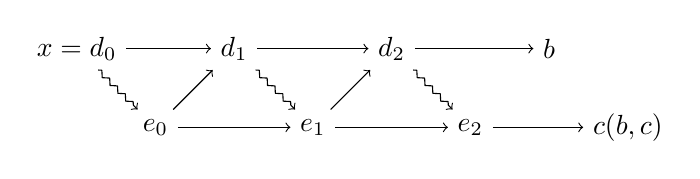
\begin{tikzpicture}[scale=1]
  \node (d0) at (0,1) {$x=d_0$};
  \node (d1) at (2,1) {$d_1$};
  \node (d2) at (4,1) {$d_2$};
  \node (b) at (6,1) {$b$};
  \node (e0) at (1,0) {$e_0$};
  \node (e1) at (3,0) {$e_1$};
  \node (e2) at (5,0) {$e_2$};
  \node (cbc) at (7,0) {$c(b,c)$};
  \draw [->, line join=round, decorate, decoration={zigzag, segment length=4, amplitude=.9,post=lineto, post length=2pt}] (d0) -- (e0);
  \draw [->, line join=round, decorate, decoration={zigzag, segment length=4, amplitude=.9,post=lineto, post length=2pt}] (d1) -- (e1);
  \draw [->, line join=round, decorate, decoration={zigzag, segment length=4, amplitude=.9,post=lineto, post length=2pt}] (d2) -- (e2);
  \draw [->] (d0) edge (d1) (d1) edge (d2) (d2) edge (b);
  \draw [->] (e0) edge (e1) (e1) edge (e2) (e2) edge (cbc);
  \draw [->] (e0) edge (d1) (e1) edge (d2);
\end{tikzpicture}
\end{center}
To see this, note first that $d_0 = x \rightsquigarrow a$, so by induction on $i$ we have $d_{i+1} = b(d_i,a) \rightsquigarrow b(a,a) = a$ for each $i$. So from $x \rightarrow b \leftarrow a$ we get $d_i \rightarrow b(d_i,a) \leftarrow a(d_i,a)$ by Claim 1, that is, $d_i \rightarrow d_{i+1} \leftarrow e_i$ for each $i$.

Then we have $e_i = a(d_i,a) \rightarrow a(d_{i+1},a) = e_{i+1}$ for each $i$, and $d_i = a(d_i,d_i) \rightsquigarrow a(d_i,a) = e_i$ for each $i$. This finishes up all of the arrows other than the rightmost two in the picture.

For $d_i \rightarrow b$, note that $d_0 = x \rightarrow b$ by assumption, and $d_{i+1} = b(d_i,a) \rightarrow b(b,b) = b$ inductively. Finally, for each $i$ we have
\[
e_i = a(d_i,a) \rightarrow c(d_i,a) \rightarrow c(b,c),
\]
where the first arrow follows from Claim 1.

Now we can use all these arrows to see that
%\[
%x = d_0 = q_1(d_0,d_0,e_0) \rightarrow q_1(d_1,e_0,e_0) = q_2(d_1,e_0,e_0) \rightarrow q_2(d_1,d_1,e_1) = q_3(d_1,d_1,e_1) \rightarrow \cdots,
%\]
\[
x = d_0 = a_0(d_0,e_0) \rightarrow b_0(d_0,e_0) \rightarrow b_0(d_1,e_0) \rightarrow a_1(d_1,e_0) \rightarrow a_1(d_1,e_1) \rightarrow b_1(d_1,e_1) \rightarrow \cdots,
\]
%where we can use squiggly arrows in the middle coordinate so long as we use solid arrows on the outer two coordinates, since each $q_i$ satisfies $q_i(x,y,x) = x$.
where we have used Claim 1 and Claim 1.5 several times. Chaining these together, we get
\[
x \rightarrow b_k(d_k,e_k) \rightarrow b_k(b,c(b,c)).%q_{2k+1}(d_k,e_k,e_k) = 
\]
This completes the proof of Claim 3.

{\bf Claim 4:} For each $i < k$, there is a $k-i$-fence
\[
x \rightarrow b_{0,i} \leftarrow a_{1,i} \rightarrow b_{1,i} \leftarrow a_{2,i} \rightarrow \cdots \leftarrow a_{k-i,i} \rightarrow b_{k-i,i} = b_k^{2^{i+1}-1}.
\]

{\bf Proof of Claim 4:} We prove this by induction on $i$. The base case $i=0$ comes from the Gumm terms. Suppose it is known for $i$, then by Claim 3 we have
\[
x \rightarrow b_k(b_{0,i},b_{1,i}(b_{0,i},b_{1,i})),
\]
and from $b_{0,i} \leftarrow x$ we have
\[
b_k(b_{0,i},b_{1,i}(b_{0,i},b_{1,i})) \leftarrow b_k(x,b_{1,i}(x,b_{1,i})) = b_k(x,b_{1,i}^2).
\]
By Claim 2, we have $b_{1,i}^2 \leftarrow a_{2,i}^2 \rightarrow b_{2,i}^2 \leftarrow \cdots$, so if we take
\[
b_{0,i+1} = b_k(b_{0,i},b_{1,i}(b_{0,i},b_{1,i}))
\]
and
\[
a_{j,i+1} = b_k(x,a_{j+1,i}^2), \;\;\; b_{j,i+1} = b_k(x,b_{j+1,i}^2),
\]
we get
\[
x \rightarrow b_{0,i+1} \leftarrow a_{1,i+1} \rightarrow b_{1,i+1} \leftarrow a_{2,i+1} \rightarrow \cdots \leftarrow a_{k-i-1,i+1} \rightarrow b_{k-i-1,i+1},
\]
and
\[
b_{k-i-1,i+1} = b_k(x,b_{k-i,i}^2) = b_k(x,(b_k^{2^{i+1}-1})^2) = b_k^{2^{i+2}-1}.
\]
This completes the proof of Claim 4.

By Claim 4 applied with $i = k-1$, we get a $1$-fence
\[
x \rightarrow b_{0,k-1} \leftarrow a_{1,k-1} \rightarrow b_{1,k-1} = b_k^{2^k-1}.
\]
Applying Claim 3, we get
\[
x \rightarrow b_k(b_{0,k-1},b_k^{2^k-1}(b_{0,k-1},b_k^{2^k-1})) = b_k^{2^k}(b_{0,k-1},b_k^{2^k-1}).
\]
Letting $b = b_{0,k-1}$, we see that we have succeeded in showing that $x \rightarrow b_k^{2^k}(b,b_k^{2^k-1})$. Thus there exist ternary terms $f_i$ with
\begin{align*}
f_1(x,x,y) &\approx x,\\
f_i(x,y,x) &\approx x\text{ for all }i,\\
f_i(x,y,y) &\approx f_{i+1}(x,x,y)\text{ for all }i,\\
f_m(x,y,y) &\approx b_k^{2^k}(b(x,y),b_k^{2^k-1}(x,y))).
\end{align*}
Note that if $b_k(x,y) = y$, then we also have $b_k^{2^k}(b(x,y),b_k^{2^k-1}(x,y))) = y$, so the above becomes a sequence of directed J\'onsson terms.

To finish, we just need to construct $p$ with $p(x,y,y) = b_k^{2^k}(b(x,y),b_k^{2^k-1}(x,y)))$ and $p(x,x,y) = y$. Recall that $p_1$ satisfied $p_1(x,y,y) = b_k(x,y)$ and $p_1(x,x,y) = y$. We construct terms $p_i$ inductively. For $2 \le i+1 < 2^k$, we set
\[
p_{i+1}(x,y,z) = p_1(x,p_i(x,y,y),p_i(x,y,z)),
\]
and for $2^k \le i+1$, we set
\[
p_{i+1}(x,y,z) = p_1(b(x,y),p_i(x,y,y),p_i(x,y,z)),
\]
and finally we set $p(x,y,z) = p_{2^{k+1}-1}(x,y,z)$.
\end{proof}

%TODO: make pictures of associated 1-IN-3 SAT instances


\section{Subdirectly irreducible algebras, ultraproducts, and residually small varieties}\label{s-subdirectly-irred}

In this section, we go over the proof of an extension of J\'onsson's Lemma \cite{jonsson-distributive}, which shows that subdirectly irreducible algebras in a finitely generated congruence distributive variety have bounded size, to the congruence modular case. The key technical tool is the concept of an ultraproduct, and the fact that any ultrapower of a finite algebra $\bA$ is isomorphic to $\bA$.

Before we discuss ultraproducts, we first review some basic results about subdirect representations of algebras due to Birkhoff \cite{birkhoff-subdirect}. The following result is elementary.

\begin{prop} If $\bA \le_{sd} \prod_{i \in I} \bA_i$ is a subdirect product, then $\bigwedge_{i \in I} \ker \pi_i = 0_\bA$. In particular, if no $\pi_i$ is an isomorphism then the congruence $0_\bA$ can be written as a meet of some family of nontrivial congruences.

Conversely, if $0_\bA$ can be written as a meet of congruences $\alpha_i \in \Con(\bA)$ for $i \in I$, then $\bA \le_{sd} \prod_{i \in I} \bA/\alpha_i$.
\end{prop}

\begin{defn} An algebraic structure $\bA$ is \emph{subdirectly irreducible} if every way of writing $\bA$ as a subdirect product $\bA \le_{sd} \prod_{i \in I} \bA_i$ has at least one coordinate $i$ such that the projection map $\pi_i : \bA \rightarrow \bA_i$ is an isomorphism. The least nontrivial congruence on a subdirectly irreducible algebra is called its \emph{monolith}.
\end{defn}

The preceeding proposition can now be rephrased as saying that $\bA$ is subdirectly irreducible iff $0_\bA$ is \emph{meet-irreducible}.

\begin{defn} An element $\alpha$ of a complete lattice $\cL$ is \emph{meet-irreducible} if for any set of elements $\alpha_i \in \cL$ with $\bigwedge_{i \in I} \alpha_i = \alpha$, some $\alpha_i$ is equal to $\alpha$. In this case, we define the \emph{cover} of $\alpha$, written $\alpha^*$, to be the least element of $\cL$ with $\alpha < \alpha^*$.
\end{defn}

In particular, the monolith of a subdirectly irreducible algebra is the cover $0_\bA^*$ of $0_\bA$.

\begin{thm}[Birkhoff's Subdirect Representation Theorem] Any algebraic structure $\bA$ can be represented as a subdirect product of subdirectly irreducible algebras.
\end{thm}
\begin{proof} For any $a\ne b \in \bA$, Zorn's Lemma implies that there is a maximal congruence $\theta_{a,b}'$ such that $(a,b) \not\in \theta_{a,b}'$. Any such $\theta_{a,b}'$ is necessarily meet-irreducible, since any congruence which properly contains $\theta_{a,b}'$ necessarily contains $(a,b)$, and therefore contains the congruence generated by $\theta_{a,b}'$ and the pair $(a,b)$.

Since we clearly have $0_\bA = \bigwedge_{a \ne b} \theta_{a,b}'$, we have the subdirect representation $\bA \le_{sd} \prod_{a \ne b} \bA/\theta_{a,b}'$.
\end{proof}

Birkhoff's subdirect representation theorem has a purely lattice-theoretic generalization to \emph{algebraic} lattices.

\begin{defn}\label{defn-algebraic-lattice} An element $\alpha$ of a complete lattice is called \emph{compact} if for any family $\alpha_i$ such that $\alpha \le \bigvee_{i \in I} \alpha_i$, there is some finite subset $\{i_1, ..., i_k\} \subseteq I$ such that $\alpha \le \alpha_{i_1} \vee \cdots \vee \alpha_{i_k}$. A complete lattice is called \emph{algebraic} if every element can be written as a join of compact elements.
\end{defn}

Every congruence lattice $\Con(\bA)$ is an algebraic lattice, since for any $a,b \in \bA$ the congruence $\theta_{a,b}$ generated by $(a,b)$ is compact, and every congruence is a join of such congruences.

\begin{prop}\label{meet-irreducible-rep} Let $\cL$ be an algebraic lattice. Then every element $\alpha$ of $\cL$ can be written as a meet of some family of meet-irreducible elements of $\cL$.
\end{prop}
\begin{proof} Let $\theta$ be any compact element of $\cL$ with $\alpha \not\ge \theta$. By Zorn's Lemma and the compactness of $\theta$, there is some $\theta' \ge \alpha$ which is maximal such that $\theta' \not\ge \theta$, and this $\theta'$ is necessarily meet-irreducible with cover $\theta' \vee \theta$. Then $\bigwedge_{\theta \not\le \alpha} \theta'$ is $\ge \alpha$, and is not $\ge$ any compact element $\theta$ with $\alpha \not\ge \theta$, so it must be equal to $\alpha$.
\end{proof}

\begin{cor}\label{meet-irreducible} If $\alpha < \beta$ in an algebraic lattice, then there is a meet-irreducible $\gamma$ such that $\gamma \ge \alpha$ but $\gamma \not\ge \beta$.
\end{cor}

Now we can briefly discuss ultrafilters and ultraproducts before moving on to the main result of this section.

\begin{defn} If $I$ is a set, then a collection of subsets $\cU \subseteq \cP(I)$ is a \emph{filter} if $\cU$ does not contain $\emptyset$, $U,V \in \cU \implies U\cap V \in \cU$, and $U \subseteq V, U \in \cU \implies V \in \cU$. We say that $\cU$ is an \emph{ultrafilter} if additionally for every $U \subseteq I$, one of $U, I\setminus U$ is in $\cU$.
\end{defn}

\begin{prop} Any filter is contained in an ultrafilter.
\end{prop}
\begin{proof} We apply Zorn's Lemma to see that any filter is contained in a maximal filter. To finish, we just need to show that any maximal filter is an ultrafilter. Suppose that $U, I\setminus U \not\in \cU$, and let $\cU'$ be the collection of $V \subseteq I$ such that $V\cup U \in \cU$. Then $\cU'$ is a filter which strictly contains $\cU$.
\end{proof}

\begin{defn} If $\bA_i$ is a collection of structures which share a common signature $\sigma$ and are indexed by $i \in I$, and if $\cU$ is an ultrafilter on $I$, then we define the \emph{ultraproduct} $\prod_i \bA_i/\cU$ to be the quotient of $\prod_i \bA_i$ by the congruence defined by
\[
a \equiv_\cU b \iff \{i \mid a_i = b_i\} \in \cU.
\]
That $\equiv_\cU$ is compatible with functions $f \in \sigma$ follows from the fact that $\cU$ is a filter. If $R \in \sigma$ is an $m$-ary relation, then $R$ is interpreted on $\prod_i \bA_i/\cU$ by
\[
R(a^1/\cU, ..., a^m/\cU) \iff \{i \mid R(a^1_i, ..., a^m_i)\} \in \cU.
\]
If all the $\bA_i$ are isomorphic to $\bA$, then we call $\bA^I/\cU$ an \emph{ultrapower} of $\bA$.
\end{defn}

Note that in terms of the congruence lattice $\Con(\prod_i \bA_i)$, the congruence $\equiv_\cU$ is equal to the join
\[
\bigvee_{U \in \cU} \ker \pi_U,
\]
where $\pi_U : \prod_{i\in I} \bA_i \rightarrow \prod_{i \in U} \bA_i$ is projection onto the coordinates in $U$. That this join is equal to the union $\bigcup_{U \in \cU} \ker \pi_U$ follows from the fact that $\cU$ is a filter.

\begin{prop} If $\cU$ is an ultrafilter on $I$ and $U_1, ..., U_k$ partition $I$ into $k$ disjoint parts, then exactly one of $U_1, ..., U_k$ is in $\cU$.
\end{prop}

\begin{cor}\label{ultraproduct-finite} If $|\bA_i| \le n$ for all $i \in I$, then $|\prod_i \bA_i/\cU| \le n$ as well. If each $\bA_i$ is finite and only finitely many isomorphism classes occur among the $\bA_i$, then $\prod_i \bA_i/\cU$ is isomorphic to some $\bA_i$.
\end{cor}

In fact, much more is true about ultraproducts, and the corollary above also follows from the following result from model theory.

\begin{thm}[{\L}o\'s's Theorem] Let $\varphi(x_1, ..., x_n)$ be any first order formula in the signature $\sigma$ with parameters $x_1, ..., x_n$, then for any $a^1, ..., a^n \in \prod_{i \in I} \bA_i$ and any ultrafilter $\cU$ on $I$, we have
\[
\prod_i \bA_i/\cU \models \varphi(a^1/\cU, ..., a^n/\cU) \iff \{i \mid \bA_i \models \varphi(a^1_i, ..., a^n_i)\} \in \cU.
\]
\end{thm}
\begin{proof} If $\varphi$ is atomic, then this follows directly from the definitions. Otherwise, $\varphi$ can be built up from atomic formulas via $\neg, \wedge, \exists$, and we can induct on the structure of $\varphi$: for $\neg$, we use the ultrafilter property that exactly one of $U, I\setminus U$ is in $\cU$ for each $U$, for $\wedge$ we use the filter property that intersections of sets in $\cU$ are in $\cU$, and for $\exists$ we just need the fact that supersets of sets in $\cU$ are in $\cU$.
\end{proof}

Now for the main result. We extend Birkhoff's $H,S,P$ notation by the operation $P_u$, where $P_u(\{\bA_i\})$ is the collection of ultraproducts of the $\bA_i$s. Recall that for $\beta$ a congruence, the centralizer $(0:\beta)$ of $\beta$ is defined as the largest $\alpha$ such that $[\alpha,\beta] = 0$, and more generally $(\delta:\beta)$ is defined as the largest $\alpha$ such that $[\alpha,\beta] \le \delta$.

\begin{thm}\label{jonsson-modular} Let $\{\bA_i\}$ be a family of algebras, and let $\cV = \cV(\{\bA_i\})$ be the variety they generate. If $\cV$ is congruence modular, $\bB \in \cV$ is subdirectly irreducible, and $\alpha = (0_\bB : 0_\bB^*)$ is the centralizer of the monolith $0_\bB^*$ of $\bB$, then $\bB/\alpha$ is a homomorphic image of a subalgebra of an ultraproduct of the $\bA_i$s, that is, $\bB/\alpha \in HSP_u(\{\bA_i\})$.
\end{thm}
\begin{proof} (From \cite{commutator-theory}, where a stronger statement is proved.) By Birkhoff's HSP Theorem, we can write $\bB = \bC/\theta$ for $\bC \le \prod_i \bA_i$. Then $\bB$ will be subdirectly irreducible iff $\theta$ is meet-irreducible in $\Con(\bC)$, so $\theta$ will have a cover $\theta^*$. The preimage $\varphi$ of $\alpha$ under $\bC \rightarrow \bB$ is the largest congruence on $\bC$ such that $[\varphi,\theta^*] \le \theta$ (i.e. $\varphi = (\theta:\theta^*)$), and we have $\bB/\alpha = \bC/\varphi$.

The main step of the proof is the following {\bf claim:} if $\beta \wedge \gamma \le \theta$ but $\gamma \not\le \theta$, then $\beta \le \varphi$.

{\bf Proof of claim:} We have
\[
[\beta,\theta^*] \le [\beta,\gamma\vee\theta] = [\beta,\gamma]\vee [\beta,\theta] \le (\beta \wedge \gamma) \vee \theta = \theta,
\]
so $\beta \le \varphi$ by $\varphi = (\theta:\theta^*)$.

Using the claim, we can now argue as follows: let $\cF$ be a maximal filter such that $U \in \cF$ implies $\ker \pi_U \le \theta$, and let $\cU$ be any ultrafilter which extends $\cF$. Then for any $U \in \cU$, we were unable to adjoin its complement to $\cF$, so there is some $V \in \cF$ such that $\ker \pi_{V\setminus U} \not\le \theta$. Then
\[
\ker \pi_U \wedge \ker \pi_{V\setminus U} = \ker \pi_{U\cup V} \le \ker \pi_V \le \theta,
\]
so by the claim we have $\ker \pi_U \le \varphi$. Thus the congruence $\bigvee_{U \in \cU} \ker \pi_U$ corresponding to $\cU$ is also $\le \varphi$, and we see that $\bB/\alpha = \bC/\varphi$ is a quotient of $\bC/\cU \le \prod_i \bA_i/\cU$.
\end{proof}

\begin{cor}[J\'onsson's Lemma \cite{jonsson-distributive}] Let $\{\bA_i\}$ be a family of algebras, and let $\cV = \cV(\{\bA_i\})$ be the variety they generate. If $\cV$ is congruence distributive and $\bB \in \cV$ is subdirectly irreducible, then $\bB \in HSP_u(\{\bA_i\})$. In particular, if $\{\bA_i\}$ is a finite set of finite algebras, then $\bB \in HS(\{\bA_i\})$.
\end{cor}

\begin{cor} For any two finite subdirectly irreducible algebras $\bA, \bB$ with the same signature which generate congruence distributive varieties, we have $\bA \cong \bB$ iff the set of identities that hold in $\bA$ is the same as the set of identities that hold in $\bB$.
\end{cor}

\begin{ex} Consider the variety of distributive lattices, and the two-element lattice $(\{0,1\},\max,\min)$. It is easy to see that every identity that holds in the two-element lattice is implied by the lattice axioms together with distributivity (since these allow us to put every term into conjunctive normal form), so the variety of distributive lattices is generated by the two-element lattice.

By J\'onsson's Lemma, the only subdirectly irreducible distributive lattice is the two-element lattice itself, so we see that in fact every distributive lattice is a sublattice of $\{0,1\}^I$ for some index set $I$, that is, every distributive lattice is a sublattice of the lattice of subsets of some set $I$.
\end{ex}

In order to understand subdirectly irreducible algebras in congruence modular varieties, we need to combine the above results with an understanding of subdirectly irreducible modules over rings.

\begin{prop} Let $\bG,\bM$ be abelian groups and let $\RR$ be a finite subgroup of $\Hom(\bG,\bM)$, such that there is a nonzero element $a \in \bM$ so that for all $x \in \bG$ there is an $r \in \RR$ with $rx = a$. Then $|\bG|$ is a prime power dividing $|\RR|$.
\end{prop}
\begin{proof} First we show that $\bG$ is finite, following \cite{commutator-theory}. Let $r_1, ..., r_k$ be the nontrivial elements of $\RR$.

We will show by induction on $k$ that $|\bG| \le (k+1)!$. For the base case, if $k = 0$ then $\bG$ can have no nonzero elements, so $|\bG| = 1 = (k+1)!$. For the inductive step, note that by the pigeonhole principle there is some $r_i$ such that at least $\frac{|\bG|-1}{k}$ elements are mapped to $a$ by $r_i$, so $|\ker r_i| \ge \frac{|\bG|-1}{k}$ (this is the ordinary group theoretic kernel), and every nonzero element of $\ker r_i$ can be mapped to $a$ by some $r_j$ with $j \ne i$, so $|\ker r_i| \le k!$ by the induction hypothesis. Thus $|\bG| \le 1 + k\cdot k! \le (k+1)!$.

Now that we know that $\bG$ is finite, we know that every element of $\bG$ has finite order, so some element $x$ has order $p$ for some prime $p$. Then there is some $r \in \RR$ with $rx = a$, so $a$ must also have order $p$. From this argument, we see that every element of $\bG$ must have order a power of $p$, so $|\bG|$ is also a power of $p$.% Suppose now that $x \in \bM$ has order $p^k$ for $k$ as large as possible, then $p^{k-1}x \ne 0$, so there is some $r \in \RR$ with $rp^{k-1}x = a$, so $rx$ has order $p^k$ and $a \in \langle rx\rangle$. Thus we can find a group theoretic isomorphism $\bM \cong \prod_i \ZZ/p^{k_i}$, with $k_1 = k$ and $a$ corresponding to a vector with $\pi_1(a) \ne 0$ under this isomorphism.

We may assume without loss of generality that $\bM$ is generated by the image of $\bG$ under all elements of $\RR$, so in particular that $\bM$ is finite. Then there exists an element $\pi \in \hat{\bM} = \Hom(\bM,\QQ/\ZZ)$ such that $\pi(a) \ne 0$.

Define a linear map $\phi : \RR \rightarrow \hat{\bG} = \Hom(\bG,\QQ/\ZZ)$ by $\phi : r \mapsto \phi_r$, where $\phi_r$ is the linear map $\phi_r: x \mapsto \pi(rx)$. Then $\phi$ must be surjective, or else the image will be a proper subgroup of $\hat{\bG}$ and so there will be some nonzero $x \in \bG$ with $\phi_r(x) = 0$ for all $r \in \RR$, which implies $rx \ne a$ for all $r$. Thus $|\bG| = |\hat{\bG}|$ divides $|\RR|$.
\end{proof}

\begin{cor} Let $\RR$ be a finite ring, and let $\bM$ be a subdirectly irreducible module over $\RR$. Then $|\bM|$ is a prime power dividing $|\RR|$.
\end{cor}
\begin{proof} If $\bM$ is subdirectly irreducible, then it has a least nontrivial submodule $\bN$, which is generated by some nonzero element $a \in \bN$. Then for each nonzero $x \in \bM$ we have $\bN \le \RR x$, so there is some $r \in \RR$ with $rx = a$. Thus we can apply the previous proposition with $\bG = \bM$.
\end{proof}

Now we can use this result to bound the sizes of subdirectly irreducible algebras in congruence modular varieties in the special case where the centralizer of the monolith is abelian.

\begin{thm}\label{subdirect-ab-prime-power} Suppose that $\bB \in \cV$ is subdirectly irreducible, and $\cV$ is locally finite and congruence modular. If $\alpha \in \Con(\bB)$ is abelian and $|\bB/\alpha| = k$, then every congruence class of $\alpha$ has size a prime power bounded by $|\cF_\cV(k+1)|$.
\end{thm}
\begin{proof} (Adapted from \cite{commutator-uses}.) Assume $\alpha$ is nontrivial, so $0_\bB^* \le \alpha$. Let $p$ be a Gumm difference term. By Corollary \ref{difference-graph}, the restriction of the graph of $p$ to the blocks of $\alpha$ is preserved by every operation of $\bB$. Choose elements $0 \ne a$ with $(0,a) \in 0_\bB^*$, and note that $0,a$ are in the same congruence block of $\alpha$.

Pick constants $c_0, ..., c_{k-1}$ with $c_0 = 0$ such that each congruence class of $\alpha$ contains some $c_i$. We will treat each congruence class $c_i/\alpha$ of $\alpha$ as an abelian group with zero element $c_i$, addition given by $x +_i y = p(x,c_i,y)$, and subtraction given by $x -_i y = p(x,y,c_i)$.

Suppose that $x \ne y$ with $(x,y) \in \alpha$. Then since $0_\bB^*$ is the least nontrivial congruence, the pair $(0,a)$ must be in the congruence generated by $(x,y)$, so there must be a chain of unary polynomials $f_i$ such that $0 = f_0(x)$, $f_i(y) = f_{i+1}(x)$, and $f_m(y) = a$. Note that this implies that $f_i(x), f_i(y)$ are all in the congruence class $0/\alpha$. Thus, it makes sense to define a unary polynomial $f$ such that
\[
f(z) = f_0(z) +_0 f_1(z) -_0 f_1(x) +_0 \cdots +_0 f_m(z) -_0 f_m(x)
\]
for $z$ in the congruence class $x/\alpha$. One explicit way to construct such an $f$ is given by
\[
f(z) = p(p(\cdots p(p(f_0(z),f_1(x),f_1(z)), f_2(x), f_2(z)), \cdots), f_m(x), f_m(z)).
\]
It's easy to check that we have $f(x) = 0$ and $f(y) = a$. Since $f$ preserves the graph of $p$ restricted to congruence classes of $\alpha$, if $x,y \in c_i/\alpha$ then we have $f(x -_i y) -_0 f(c_i) = a$, and the unary polynomial $z \mapsto f(z) -_0 f(c_i)$ defines a linear map in $\Hom(c_i/\alpha, c_0/\alpha)$.

To finish, we just need to bound the size of the subgroup $\RR_{i,0}$ of linear maps in $\Hom(c_i/\alpha, c_0/\alpha)$ which can be defined by unary polynomials $f$. Suppose that $f(z) = t(z,b_1, ..., b_m)$ for some term $t$ and constants $b_1, ..., b_m \in \bB$, such that $f(c_i) = c_0$. For each $b_i$, we choose $j_i$ such that $b_i \in c_{j_i}/\alpha$. Define a unary polynomial $f'$ by
\[
f'(z) = t(z,c_{j_1}, ..., c_{j_m}) -_0 t(c_i, c_{j_1}, ..., c_{j_m}).
\]
Then for $z \in c_i/\alpha$, we have $f'(z) \in c_0/\alpha$, and since $t$ preserves the graph of $p$ restricted to congruence classes of $\alpha$, we have $f'(z) = f(z)$ for $z \in c_i/\alpha$ (alternatively, we could prove this by the term condition for $[\alpha,\alpha] = 0_\bB$). Thus every element of $\Hom(c_i/\alpha,c_0/\alpha)$ which can be defined by a unary polynomial can also be defined by a polynomial $f'$ which has the form $f'(z) = t'(z,c_0,...,c_{k-1})$ for some $k+1$-ary term $t'$, so
\[
|\RR_{i,0}| \le |\cF_\cV(k+1)|.
\]
Applying the previous proposition, we see that $|c_i/\alpha|$ is a prime power dividing $|\RR_{i,0}|$.
\end{proof}

\begin{cor}\label{subdirect-bound-ab} If $|\bA| = m$ is finite and $\cV(\bA)$ is congruence modular, and if $\bB \in \cV(\bA)$ is subdirectly irreducible with $(0_\bB:0_\bB^*)$ abelian, then $|\bB| \le m\cdot m^{m^{m+1}}$.
\end{cor}

\begin{defn} A variety $\cV$ is called \emph{residually small} if there is a cardinal $\kappa$ such that every subdirectly irreducible algebra $\bB \in \cV$ has $|\bB| < \kappa$, and \emph{residually finite} if every subdirectly irreducible algebra in $\cV$ is finite. An algebra $\bA$ is called residually small if the variety $\cV(\bA)$ generated by $\bA$ is residually small.
\end{defn}

First we show that if a locally finite variety contains an infinite subdirectly irreducible algebra, then it contains infinitely many distinct finite subdirectly irreducible algebras.

\begin{thm}\label{ultraproduct-fin-gen} If $\bB$ is subdirectly irreducible, then $\bB$ is a subalgebra of an ultraproduct of a family of finitely generated subdirectly irreducible algebras in $HS(\bB)$.
\end{thm}
\begin{proof} (From \cite{commutator-theory}.) Let the monolith $0_\bB^*$ of $\bB$ be generated (as a congruence) by the pair $(a,b)$. Let $I$ be the family of finitely generated subalgebras $\bS \le \bB$ with $a,b \in \bS$, and for each $\bS \in I$, pick a congruence $\alpha_\bS$ on $\bS$ which is maximal among all congruences which do not contain $(a,b)$. Then each $\bS/\alpha_\bS$ is subdirectly irreducible, since every congruence which properly contains $\alpha_\bS$ contains $(a,b)$.

Let $\cU$ be an ultrafilter on $I$ such that the set $U_S = \{\bS \mid S \subseteq \bS\}$ is in $\cU$ for every finite $S \subseteq \bB$. Such an ultrafilter exists since for any $S_1, S_2$ we have $U_{S_1} \cap U_{S_2} = U_{S_1\cup S_2}$, and for $S$ finite $U_S$ is nonempty since it contains $\Sg_\bB(S \cup \{a,b\})$.

Define a map $\varphi : \bB \rightarrow (\prod_{\bS \in I} \bS/\alpha_\bS)/\cU$ as the ultraproduct of the family of maps $\varphi_\bS$ given by $\varphi_\bS(x) = x/\alpha_\bS$ for $x \in \bS$ and $\varphi_\bS(x) = a/\alpha_\bS$ for $x \not\in \bS$. Then for $x_1, ..., x_k \in \bB$ and $t$ a $k$-ary term of $\bB$, we have
\[
\{\bS \mid \varphi_\bS(t(x_1, ..., x_k)) = t(\varphi_\bS(x_1), ..., \varphi_\bS(x_k))\} \in \cU,
\]
since it contains $U_{\{x_1, ..., x_k\}}$. Thus $\varphi$ is a homomorphism. To see that it is injective, just note that $\varphi_\bS(a) \ne \varphi_\bS(b)$ for all $\bS \in I$.
\end{proof}

\begin{cor}\label{residually-infinite} If a locally finite variety contains an infinite subdirectly irreducible algebra, then it contains arbitrarily large finite subdirectly irreducible algebras.
\end{cor}

It turns out that finite residually small algebras can be understood in terms of a commutator condition. We say that an algebra $\bA$ satisfies a commutator identity \emph{hereditarily} if every congruence lattice of every subalgebra of $\bA$ satisfies the identity.

\begin{prop} The commutator identity $[\alpha \wedge \beta, \beta] = \alpha \wedge [\beta,\beta]$ is equivalent to the implication $\alpha \le [\beta,\beta] \implies [\alpha,\beta] = \alpha$.
\end{prop}
\begin{proof} The implication clearly follows from the identity. For the other direction, we apply the implication to $\alpha \wedge [\beta,\beta] \le [\beta,\beta]$ to see that
\[
\alpha \wedge [\beta,\beta] = [\alpha \wedge [\beta,\beta], \beta] \le [\alpha\wedge \beta,\beta] \le \alpha \wedge [\beta,\beta].\qedhere
\]
\end{proof}

\begin{prop} If $\bA$ is in a congruence modular variety and satisfies the commutator identity $[\alpha \wedge \beta,\beta] = \alpha \wedge [\beta,\beta]$ hereditarily, then so does every quotient $\bB$ of $\bA$.
\end{prop}
\begin{proof} Suppose $\bB = \bA/\gamma$ and $\alpha,\beta \in \Con(\bA)$ with $\alpha,\beta \ge \gamma$. We need to check that if $\alpha \le [\beta,\beta]_\gamma$, then $\alpha = [\alpha,\beta]_\gamma$. By the modular law, if $\alpha \le [\beta,\beta]\vee \gamma$ then
\[
\alpha = \alpha \wedge ([\beta,\beta]\vee \gamma) = (\alpha \wedge [\beta,\beta]) \vee \gamma = [\alpha,\beta] \vee \gamma = [\alpha,\beta]_\gamma.\qedhere
\]
\end{proof}

\begin{prop} If $\bA_1,\bA_2$ are in a congruence modular variety and satisfy the commutator identity $[\alpha\wedge \beta, \beta] = \alpha\wedge [\beta,\beta]$ hereditarily, then so does their product $\bA_1 \times \bA_2$.
\end{prop}
\begin{proof} Let $\bB \le \bA_1\times \bA_2$, we can assume without loss of generality that this inclusion is subdirect by replacing the $\bA_i$ with $\pi_i(\bB)$. Suppose $\alpha,\beta \in \Con(\bB)$ with $\alpha \le [\beta,\beta]$, we will show that $[\alpha,\beta] = \alpha$. We have
\[
\alpha \vee \ker\pi_1 \le [\beta\vee\ker\pi_1, \beta\vee\ker\pi_1]_{\ker \pi_1},
\]
so from the assumption on $\bA_1$ we get
\[
\alpha \vee \ker \pi_1 = [\alpha \vee \ker\pi_1, \beta \vee \ker \pi_1]_{\ker \pi_1} = [\alpha,\beta]\vee \ker \pi_1.
\]
Thus by the modular law and $[\alpha,\beta] \le \alpha$, we have
\[
\alpha = \alpha\wedge (\ker \pi_1 \vee [\alpha,\beta]) = (\alpha \wedge \ker \pi_1) \vee [\alpha,\beta].
\]
Similarly, we have $\alpha = (\alpha \wedge \ker \pi_2) \vee [\alpha,\beta]$. Since $\alpha \wedge \ker \pi_2 \le \alpha \le [\beta,\beta]$, we may apply the same reasoning to $\alpha \wedge \ker \pi_2$ to see that
\[
\alpha \wedge \ker \pi_2 = (\alpha \wedge \ker \pi_2 \wedge \ker \pi_1) \vee [\alpha \wedge \ker \pi_2, \beta],
\]
so $\alpha \wedge \ker \pi_2 \le [\alpha,\beta]$, so
\[
\alpha = (\alpha \wedge \ker \pi_2) \vee [\alpha,\beta] = [\alpha,\beta].\qedhere
\]
\end{proof}

\begin{thm} If $|\bA| = m$ is finite and $\cV(\bA)$ is congruence modular, and if $\bA$ satisfies the commutator identity $[\alpha \wedge \beta,\beta] = \alpha \wedge [\beta,\beta]$ hereditarily, then every subdirectly irreducible algebra $\bB \in \cV(\bA)$ has $|\bB| \le m\cdot m^{m^{m+1}}$.
\end{thm}
\begin{proof} By Corollary \ref{residually-infinite}, we just need to check the bound in the case where $\bB$ is finite. In this case, we have $\bB \in HSP_{fin}(\bA)$, so $\bB$ satisfies the commutator identity $[\alpha \wedge \beta,\beta] = \alpha \wedge [\beta,\beta]$ by the previous propositions. Let $0_\bB^*$ be the monolith of $\bB$, and let $\alpha = (0_\bB:0_\bB^*)$ be its centralizer.

We claim that $\alpha$ is abelian. To see this, note that from $[\alpha,0_\bB^*] = 0_\bB$ we have
\[
0_\bB = [0_\bB^*\wedge \alpha,\alpha] = 0_\bB^*\wedge [\alpha,\alpha],
\]
so $[\alpha,\alpha] = 0_\bB$. Now we can apply Corollary \ref{subdirect-bound-ab} to see that $|\bB| \le m\cdot m^{m^{m+1}}$.%If not, then $0_\bB^* \le [\alpha,\alpha]$, so $[0_\bB^*,\alpha] = 0_\bB^*$, contradicting the fact that $\alpha$ is the centralizer of $0_\bB^*$.
\end{proof}

\begin{ex} The symmetric group $S_3$ on three letters is residually small, since it satisfies the commutator identity $[\alpha \wedge \beta, \beta] = \alpha \wedge [\beta,\beta]$ hereditarily: the only interesting case to check is that $[A_3,S_3] = A_3$, where $A_3$ is the alternating group on three letters. We have $HS(S_3) = \{1, \ZZ/2, \ZZ/3, S_3\}$, and all three nontrivial elements are subdirectly irreducible.

The general theory shows that every subdirectly irreducible $\bG \in \cV(S_3)$ has an abelian normal subgroup $\bN$ with $\bG/\bN \in HS(S_3)$, with $|\bN|$ a prime power bounded by $|\cF_{\cV(S_3)}(|\bG/\bN|+1)| \le 6^{6^7}$. Since $\bN \in \cV(S_3)$ and every element of $S_3$ has order dividing $6$, $\bN$ has exponent $2$ or $3$. From here it is not too hard to check that the only nontrivial subdirectly irreducible algebras in $\cV(S_3)$ are $\ZZ/2,\ZZ/3, S_3$, and all three of these are subgroups of $S_3$. Thus every group in $\cV(S_3)$ is a subgroup of a power of $S_3$.
\end{ex}

\begin{prop} If $\bA$ is contained in a congruence modular variety but does not satisfy the commutator identity $[\alpha \wedge \beta,\beta] = \alpha \wedge [\beta,\beta]$ hereditarily, then there is some subdirectly irreducible $\bB \in HS(\bA)$ such that the centralizer of the monolith of $\bB$ is not abelian.
\end{prop}
\begin{proof} Suppose that $\bA$ fails to satisfy the commutator identity. In this case there must be $\alpha, \beta \in \Con(\bA)$ with $\alpha \le [\beta,\beta]$ and $[\alpha,\beta] < \alpha$. Let $\theta$ be a meet-irreducible congruence such that $\theta \ge [\alpha,\beta]$ but $\theta \not\ge \alpha$, and let $\theta^*$ be its cover. Then
\[
\theta^* \le \alpha\vee\theta \le [\beta,\beta]\vee \theta \le [\beta\vee\theta,\beta\vee\theta]_\theta
\]
and
\[
[\theta^*,\beta\vee\theta]_\theta \le [\alpha\vee\theta,\beta\vee\theta]_\theta = [\alpha,\beta]\vee\theta = \theta,
\]
so if we take $\bB$ to be $\bA/\theta$, then the monolith of $\bB$ is $\theta^*/\theta$, and $\beta\vee\theta/\theta$ is contained in the centralizer of the monolith of $\bB$ but is not abelian.
\end{proof}

\begin{thm} If $\bA$ is contained in a congruence modular variety but does not satisfy the commutator identity $[\alpha \wedge \beta,\beta] = \alpha \wedge [\beta,\beta]$, then $\cV(\bA)$ is not residually small. In fact, for every cardinal $\kappa$, $\cV(\bA)$ contains a subdirectly irreducible algebra whose congruence lattice has size at least $\kappa$.
\end{thm}
\begin{proof} (From \cite{commutator-theory}.) By the proposition, we can reduce to the case where $\bA$ is subdirectly irreducible and the centralizer $\beta$ of the monolith $0^*$ is not abelian.

Consider $\beta$ as a subalgebra of $\bA^2$, and $\Delta_\beta^{0^*}$ as a congruence on $\beta$. From $[\beta,0_\bA^*] = 0_\bA$ we have $\Delta_\beta^{0^*} \wedge \ker \pi_1 = \Delta_\beta^{0^*} \wedge \ker \pi_2 = 0_\beta$, and from the definition of $\Delta_\beta^{0^*}$ we have $\Delta_\beta^{0^*} \vee \ker \pi_i = \pi_i^{-1}(0^*)$. Set $0^*_i = \pi_i^{-1}(0^*)$ and $\theta = 0^*_1 \wedge 0^*_2, \theta_i = 0^*_i \wedge \ker \pi_{\{1,2\}\setminus \{i\}}$, then (after several applications of the modular law - don't worry about the details just yet) we have the following sublattice in $\Con(\beta)$.
\begin{center}
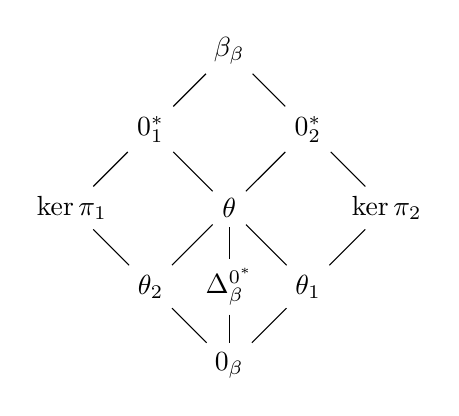
\begin{tikzpicture}[scale=1.0]
  \node (1) at (0,2) {$\beta_{\beta}$};
  \node (01) at (-1,1) {$0^*_1$};
  \node (02) at (1,1) {$0^*_2$};
  \node (p1) at (-2,0) {$\ker \pi_1$};
  \node (c) at (0,0) {$\theta$};
  \node (p2) at (2,0) {$\ker \pi_2$};
  \node (t1) at (-1,-1) {$\theta_2$};
  \node (t2) at (1,-1) {$\theta_1$};
  \node (d) at (0,-1) {$\Delta_\beta^{0^*}$};
  \node (0) at (0,-2) {$0_\beta$};
  \draw (1) -- (01) -- (p1) -- (t1) -- (0) -- (t2) -- (p2) -- (02) -- (1);
  \draw (01) -- (c) -- (02);
  \draw (t1) -- (c) -- (t2);
  \draw (c) -- (d) -- (0);
\end{tikzpicture}
\end{center}
In the picture, we see that $\Delta_\beta^{0^*}$ appears to be meet-irreducible in $\Con(\beta)$, and the interval $\llbracket \Delta_\beta^{0^*}, \beta_\beta\rrbracket$ contains the incomparable elements $0^*_1, 0^*_2$. If $\Delta_\beta^{0^*}$ isn't meet-irreducible, we can still try to find a meet-irreducible congruence $\lambda$ on $\beta$ which is above $\Delta_\beta^{0^*}$ but not above $\theta$, and then $\beta/\lambda$ should give us a subdirectly irreducible algebra whose congruence lattice contains two distinct elements coming from $\ker \pi_1 \vee \lambda$ and $\ker \pi_2 \vee \lambda$ (that neither of these is equal to $\beta_\beta$ will come from the assumption that $\beta$ is not abelian). This is the basic idea behind the general construction, but we will need to scale up by considering higher dimensional analogues of $\beta \le \bA^2$.

Let $\kappa$ be any cardinal, considered as the set of all ordinals below $\kappa$. Define $\bB \le \bA^\kappa$ by
\[
\bB = \{a \in \bA^\kappa \mid a_i \equiv_\beta a_j\ \forall i,j \in \kappa\}.
\]
Then $\bB$ has a natural map to $\bA/\beta$, and we call the kernel of this map $\beta_\bB$. Inside $\Con(\bB)$, we have $\ker \pi_i \vee \ker \pi_j = \beta_\bB$ for all $i \ne j \in \kappa$. The strategy is to construct a congruence $\lambda$ on $\bB$ such that $\bB/\lambda$ is subdirectly irreducible and $\ker \pi_i \vee \lambda \not\ge \beta_\bB$ for all $i$, which will guarantee that the congruences $\ker \pi_i \vee \lambda/\lambda \in \Con(\bB/\lambda)$ are pairwise distinct. The congruence $\lambda$ will be constructed by first constructing congruences $\Delta, \theta$ with $\Delta < \theta$ and $\theta \vee \ker \pi_i \not\ge \beta_\bB$.

We need a congruence on $\bB$ generalizing $\Delta_\beta^{0^*}$ on $\beta$. We define $\Delta_i$ by
\[
(a,b) \in \Delta_i \iff \begin{bmatrix} a_0 & b_0\\ a_i & b_i\end{bmatrix} \in \Delta_\beta^{0^*} \wedge (a_j = b_j\ \forall j \ne 0,i),
\]
and define $\Delta$ by
\[
\Delta = \bigvee_{0 < i < \kappa} \Delta_i.
\]
We also define congruences $\theta_i$ by
\[
(a,b) \in \theta_i \iff (a_i,b_i) \in 0_\bA^* \wedge (a_j = b_j\ \forall j \ne i),
\]
and define $\theta$ by
\[
\theta = \bigvee_{i < \kappa} \theta_i.
\]

We need to check some basic properties of these congruences, to see that they behave as in the picture of $\Con(\beta)$. First, we check that $\theta_0 \le \theta_i \vee \Delta_i$ for all $i$. Letting $\pi_{i'}$ be the projection onto all coordinates other than $i$, then it's easy to check that $\theta_0 \le \ker \pi_{i'} \vee \Delta$ by reasoning about just the two coordinates $0,i$ and keeping all other coordinates fixed:
\[
\begin{bmatrix} a_0\\ a_i\end{bmatrix}\ \ker \pi_{i'}\ \begin{bmatrix} a_0\\ a_0\end{bmatrix}\ \Delta_i\ \begin{bmatrix} b_0\\ b_0\end{bmatrix}\ \ker \pi_{i'}\ \begin{bmatrix} b_0\\ b_i\end{bmatrix}.
\]
Then by the modular law, if we let $0^*_i = \pi_i^{-1}(0^*_\bA)$ and note that $\Delta_i \le 0^*_i$, we get
\[
\theta_0 = \theta_0 \wedge 0^*_i \le (\Delta_i \vee \ker \pi_{i'}) \wedge 0^*_i = \Delta_i \vee (\ker \pi_{i'} \wedge 0^*_i) = \Delta_i \vee \theta_i.
\]
Similarly, we get $\theta_i \le \theta_0 \vee \Delta_i$ for all $i$.

Next, for each $i$ we have $\Delta \vee \theta_i = \theta$: for each $j \in \kappa$, we have
\[
\Delta \vee \theta_i = \Delta \vee \Delta_i \vee \theta_i \ge \Delta \vee \theta_0 \ge \Delta_j \vee \theta_0 \ge \theta_j,
\]
so $\Delta \vee \theta_i \ge \bigvee_{j \in \kappa} \theta_j = \theta$, while the other containment follows from $\Delta_i \le \theta_0 \vee \theta_i$ for all $i$.

We now check that $\Delta \ne \theta$. It's enough to check that $\theta_0 \not\le \Delta$, since $\Delta \vee \theta_0 = \theta$. Note first that $\theta_0$ is compact, since $0^*_\bA$ is compact. Thus we just need to check that $\theta_0 \not\le \bigvee_{j \le n} \Delta_{i_j}$ for all $i_1, ..., i_n$. In fact, we can assume that $i_1, ..., i_n$ are $1, ..., n$ by a symmetry argument.

We will show by induction on $n$ that $\theta_0\wedge (\Delta_1 \vee \cdots \vee \Delta_n) = 0_\bB$ for all $n$. The base case follows from the fact that $[\beta,0^*_\bA] = 0_\bA \implies \ker \pi_2 \wedge \Delta_\beta^{0^*} = 0_\beta$ in $\Con(\beta)$, which in turn implies $\theta_0 \wedge \Delta_1 = 0_\bB$. For the inductive step, we argue as follows:
\begin{align*}
\theta_0\wedge (\Delta_1 \vee \cdots \vee \Delta_n) &= \theta_0\wedge (\theta_0\vee \theta_n)\wedge (\Delta_1 \vee \cdots \vee \Delta_n)\\
&= \theta_0 \wedge (((\theta_0\vee \theta_n) \wedge (\Delta_1 \vee \cdots \vee \Delta_{n-1})) \vee \Delta_n)\\
&= \theta_0 \wedge ((\theta_0 \wedge (\Delta_1 \vee \cdots \vee \Delta_{n-1})) \vee \Delta_n)\\
&= \theta_0 \wedge \Delta_n = 0_\bB,
\end{align*}
where the second equality used the modular law and the fact that $\Delta_n \le \theta_0\vee \theta_n$, the third equality used the fact that $\theta_n$ is independent of everything that happens on the coordinates $0, ..., n-1$, and the last two equalities used the inductive hypothesis.

We have shown that $\Delta < \theta$. We can now apply Corollary \ref{meet-irreducible} to see that there is some meet-irreducible congruence $\lambda$ with $\lambda \ge \Delta$ but $\lambda \not\ge \theta$. To finish, we just need to check that $\lambda \vee \ker \pi_i \not\ge \beta_\bB$. To see this, note that $\lambda \not\ge \theta_i$, since otherwise we would have $\lambda \ge \Delta \vee \theta_i = \theta$, a contradiction. Since $\theta_i$ is the minimal nonzero element of the interval $\llbracket 0_\bB, \ker \pi_{i'}\rrbracket$, this means that $\lambda \wedge \ker \pi_{i'} = 0_\bB$. Thus if (for contradiction) $\lambda \vee \ker \pi_i \ge \beta_\bB$, then we would have
\[
[\beta_\bB, \beta_\bB] \le [\ker \pi_{i'} \vee \ker \pi_i, \lambda \vee \ker \pi_i] \le (\lambda \wedge \ker \pi_{i'}) \vee \ker \pi_i = \ker \pi_i,
\]
and applying $\pi_i$ we would get $[\beta,\beta] = 0_\bA$, a contradiction to the assumption that $\beta$ was not abelian.

Putting it all together, we have a meet-irreducible congruence $\lambda$ such that $\lambda \vee \ker \pi_i \not\ge \beta_\bB$ for each $i$, but $\ker \pi_i \vee \ker \pi_j \ge \beta_\bB$ for all $i \ne j$. Thus $\bB/\lambda$ is subdirectly irreducible, and the congruences $\ker \pi_i \vee \lambda/\lambda$ are mutually distinct elements of $\Con(\bB/\lambda)$.
\end{proof}

\begin{cor}\label{residual-crit} Let $\cV$ be a finitely generated congruence modular variety. Then the following are equivalent:
\begin{itemize}
\item $\cV$ is residually small,

\item every algebra in $\cV$ satisfies the commutator identity $[\alpha \wedge \beta, \beta] = \alpha \wedge [\beta,\beta]$,

\item $\cV$ is generated by a finite algebra $\bA$ such that for every subdirectly irreducible $\bB \in HS(\bA)$, the centralizer of the monolith of $\bB$ is abelian,

\item $\cV$ is generated by a finite algebra which satisfies the commutator identity $[\alpha \wedge \beta, \beta] = \alpha \wedge [\beta,\beta]$ hereditarily,

\item $\cV$ has a finite bound on the size of its subdirectly irreducible elements.
\end{itemize}
\end{cor}

\begin{cor} If $\bA$ is in a congruence modular variety and has size $|\bA| \le 3$, then $\cV(\bA)$ is residually small.
\end{cor}
\begin{proof} Suppose for contradiction that $\bA$ is subdirectly irreducible with a monolith $0_\bA^*$ whose centralizer $(0_\bA : 0_\bA^*)$ is not abelian. Then since $\Con(\bA)$ has height at most $2$, we necessarily have
\[
0_\bA < 0_\bA^* < (0_\bA : 0_\bA^*) = 1_\bA.
\]
Thus $|\bA| = 3$, and we may name the elements of $\bA$ as $a,b,c$, such that $0_\bA^*$ corresponds to the partition $\{a,b\},\{c\}$ of $\bA$. Letting $p(x,y,z)$ be a Gumm difference term, we see from Theorem \ref{difference-commutator} that
\[
\begin{bmatrix} a & p(a,b,c)\\ b & c\end{bmatrix} \in \Delta_{0_\bA^*}^{1_\bA}.
\]
Modulo $0_\bA^*$, we have $p(a,b,c) \equiv_{0_\bA^*} p(a,a,c) = c$, so we must have $p(a,b,c) = c$. Then by Theorem \ref{shifting-commutator} we have $(a,b) \in [1_\bA, 0_\bA^*]$, which contradicts $(0_\bA : 0_\bA^*) = 1_\bA$.
\end{proof}

\begin{prop}\label{residual-nilpotent} If $\bA$ satisfies the commutator identity $[\alpha\wedge \beta,\beta] = \alpha \wedge [\beta,\beta]$, then every nilpotent congruence on $\bA$ is abelian.
\end{prop}
\begin{proof} The commutator identity implies that
\[
[[\alpha,\alpha],\alpha] = [[\alpha,\alpha] \wedge \alpha,\alpha] = [\alpha,\alpha]\wedge[\alpha,\alpha] = [\alpha,\alpha].\qedhere
\]
\end{proof}

\begin{prop}[Ol'{\v{s}}anski{\u\i} \cite{residually-small-groups}]\label{sylow-abelian} If all the Sylow subgroups of a finite group $\bG$ are abelian, then the center $Z(\bG)$ and the commutator subgroup $[\bG,\bG]$ intersect trivially, that is, $Z(\bG) \wedge [\bG,\bG] = 0_\bG$.
\end{prop}
\begin{proof} Fix a Sylow subgroup $\bS$ of $\bG$, and consider the transfer map $\bG \rightarrow \bS/[\bS,\bS]$. Recall that the transfer homomorphism from a finite group to the abelianization of a subgroup is defined by making a choice of coset representatives $x_i$ with $\bG = \bigcup_i x_i\bS$, and sending $g \in \bG$ to $\prod_i s_i/[\bS,\bS]$, where for each $i$, $s_i \in \bS$ is given by $gx_i = x_js_i$ for some $j$. Since $\bS$ is assumed to be abelian, this gives us a homomorphism from $\bG$ to $\bS$.

Now consider any $g \in Z(\bG) \cap \bS$. The transfer homomorphism sends $g$ to $\prod_i g = g^{[\bG:\bS]}$ since $gx_i = x_ig$ for each $i$, and if $g \ne 1$ then $g^{[\bG:\bS]} \ne 1$ as well since $[\bG:\bS]$ is relatively prime to the order of $g$. Thus there is a map from $\bG$ to an abelian group such that $g$ is not in the kernel, so $g \not\in [\bG,\bG]$. Since every nontrivial element of $Z(\bG) \wedge [\bG,\bG]$ has a power which has prime order and is therefore contained in a Sylow subgroup of $\bG$, we must have $Z(\bG) \wedge [\bG,\bG] = 0_\bG$ to avoid a contradiction.
\end{proof}

\begin{cor}[Ol'{\v{s}}anski{\u\i} \cite{residually-small-groups}] A finite group is residually small iff all of its Sylow subgroups are abelian.
\end{cor}
\begin{proof} By Proposition \ref{residual-nilpotent}, all nilpotent subgroups of a finite residually small group must be abelian, so in particular the Sylow subgroups must be abelian since all $p$-groups are nilpotent.

For the other direction, note that for any $\bB \in HS(\bA)$, the Sylow subgroups of $\bB$ are quotients of subgroups of the Sylow subgroups of $\bA$ by the Sylow theorems. Thus we just have to check that if the Sylow subgroups of a subdirectly irreducible group are abelian, then the centralizer $\bC$ of its  monolith $0^*$ is abelian.

Note that if $\bC$ centralizes $0^*$, then $0^* \le Z(\bC)$. By Proposition \ref{sylow-abelian}, we have $Z(\bC) \wedge [\bC,\bC] = 0$, so $0^* \wedge [\bC,\bC] = 0$, which implies that $[\bC,\bC] = 0$.
\end{proof}

\subsection{Similarity}\label{ss-similarity}

Even if a finitely generated congruence modular variety is not residually small, we can still classify its subdirectly irreducible algebras by using the concept of \emph{similarity} from Freese and McKenzie \cite{commutator-theory}. We will use a different definition of similarity than their definition, but which they prove to be equivalent.

\begin{defn} We say that subdirectly irreducible algebras $\bA, \bB$ in a congruence modular variety $\cV$ are \emph{similar} if there exists an algebra $\bC \in \cV$ with congruences $\alpha, \beta, \gamma, \delta \in \bC$ such that $\bC/\alpha \cong \bA$, $\bC/\beta \cong \bB$, and
\[
\llbracket \alpha, \alpha^* \rrbracket \searrow \llbracket \gamma, \delta \rrbracket \nearrow \llbracket \beta, \beta^* \rrbracket.
\]
If furthermore $\bC \le_{sd} \bA\times \bB$ and $\alpha, \beta$ are the kernels of the projections to $\bA,\bB$, then we say that $\bC$ is the \emph{graph of a similarity} from $\bA$ to $\bB$.
\end{defn}

\begin{prop}\label{similarity-graph} If $\bA, \bB$ are similar, then there is a witnessing algebra $\bC \le_{sd} \bA\times\bB$ which is the graph of a similarity from $\bA$ to $\bB$. If $\alpha,\beta$ are the kernels of the projections to $\bA,\bB$, then $(\alpha:\alpha^*) = (\beta:\beta^*)$ and $\bC/(\alpha:\alpha^*)$ is the graph of an isomorphism
\[
\bA/(0_\bA:0_\bA^*) \xrightarrow{\sim} \bB/(0_\bB:0_\bB^*).
\]
If $\bA, \bB$ are similar but not isomorphic, then they must both have abelian monoliths.
\end{prop}
\begin{proof} For the first statement, let $\bC \in \cV$ and $\alpha,\beta,\gamma,\delta \in \Con(\bC)$ be as in the definition of similarity. It's enough to show that we have
\[
\llbracket \alpha, \alpha^* \rrbracket \searrow \llbracket \alpha\wedge\beta, (\alpha\wedge\beta)\vee \delta \rrbracket \nearrow \llbracket \beta, \beta^* \rrbracket,
\]
since then we can replace $\bC$ by $\bC/(\alpha\wedge\beta)$, which is a subdirect product of $\bC/\alpha \cong \bA$ and $\bC/\beta \cong \bB$. We have
\[
\alpha \vee ((\alpha\wedge\beta)\vee \delta) = \alpha\vee\delta = \alpha^*,
\]
and by the modular law and the fact that $\gamma \le \alpha \wedge \beta$, we have
\[
\alpha \wedge ((\alpha\wedge\beta)\vee \delta) = (\alpha \wedge \delta) \vee (\alpha \wedge \beta) = \gamma \vee (\alpha \wedge \beta) = (\alpha \wedge \beta),
\]
so $\llbracket \alpha, \alpha^* \rrbracket \searrow \llbracket \alpha\wedge\beta, (\alpha\wedge\beta)\vee \delta \rrbracket$, and the other perspectivity follows by a symmetric argument.

The remaining statements follow from the Diamond Isomorphism Theorem \ref{diamond-isom}: if $\llbracket \alpha, \alpha^* \rrbracket \searrow \llbracket \gamma, \delta \rrbracket \nearrow \llbracket \beta, \beta^* \rrbracket$, then $(\alpha:\alpha^*) = (\gamma:\delta) = (\beta:\beta^*)$, so
\[
\bA/(0_\bA:0_\bA^*) \cong \bC/(\alpha:\alpha^*) = \bC/(\beta:\beta^*) \cong \bB/(0_\bB:0_\bB^*),
\]
and
\[
[\alpha^*,\alpha^*]_\alpha = \alpha \iff [\delta,\delta]_\gamma = \gamma \iff [\beta^*,\beta^*]_\beta = \beta,
\]
so $0_\bA^*$ is abelian iff $0_\bB^*$ is abelian, and if neither is abelian then $\alpha = (\alpha:\alpha^*) = (\beta:\beta^*) = \beta$ and $\bA \cong \bC/\alpha = \bC/\beta \cong \bB$.
\end{proof}

\begin{prop} If $\bA, \bB$ are similar such that $\sigma$ is the corresponding isomorphism
\[
\sigma: \bA/(0_\bA:0_\bA^*) \xrightarrow{\sim} \bB/(0_\bB:0_\bB^*),
\]
then they are similar via the algebra $\RR = \{(x,y) \in \bA \times \bB \mid \sigma(x/(0_\bA:0_\bA^*)) = y/(0_\bB:0_\bB^*)\}$.
\end{prop}
\begin{proof} Suppose $\bC \le \RR$ is the graph of a similarity from $\bA$ to $\bB$, with
\[
\llbracket \ker \pi_1, (\ker \pi_1)^* \rrbracket \searrow \llbracket 0_\bC, \delta \rrbracket \nearrow \llbracket \ker \pi_2, (\ker \pi_2)^* \rrbracket
\]
in $\Con(\bC)$. We may assume that $\bA, \bB$ have abelian monoliths, so $[\delta,\delta] = 0_\bC$ by the Diamond Isomorphism Theorem \ref{diamond-isom}. Then by Theorem \ref{commutator-permute}, $\delta$ permutes with all congruences in $\Con(\bC)$, so in particular $(\ker \pi_1)^* = \delta \circ \ker \pi_1$. In other words, for any $(a,b) \in \bC$ and any $a' \in a/0_\bA^*$, there exists a $b'$ such that
\[
\begin{bmatrix} a\\ b\end{bmatrix}\ \delta\ \begin{bmatrix} a'\\ b'\end{bmatrix}.
\]
In fact, this $b'$ is uniquely determined by $a,b,a'$, since $\delta \wedge \ker \pi_1 = 0_\bC$. Additionally, we must have $b' \in b/0_\bB^*$, since $\delta \le (\ker \pi_2)^*$.

Now we can extend $\delta$ to a congruence $\delta_\RR \in \Con(\RR)$ as follows. For $(a,b), (a',b') \in \RR$ with $a\ 0_\bA^*\ a'$ and $b\ 0_\bB^*\ b'$, we pick any $(u,v) \in \bC$ with $u\ (0_\bA:0_\bA^*)\ a$ and write
\[
\begin{bmatrix} a & a'\\ b & b'\end{bmatrix} \in \delta_\RR\ \iff\ \begin{bmatrix} p(a,a',u) & u\\ p(b,b',v) & v\end{bmatrix} \in \delta,
\]
where $p$ is a Gumm difference term. Note that by Corollary \ref{difference-graph}, this choice of $\delta_\RR$ is preserved by the operations of $\bA$ so long as it is well-defined. To check that this is in independent of the choice of $(u,v) \in \bC$, suppose $(u',v') \in \bC$ with $u'\ (0_\bA:0_\bA^*)\ a$, and apply Corollary \ref{difference-graph} again to see that
\[
p\left(\begin{bmatrix} p(a,a',u) & u\\ p(b,b',v) & v\end{bmatrix}, \begin{bmatrix} p(a,a,u) & u\\ p(b,b,v) & v\end{bmatrix}, \begin{bmatrix} p(a,a,u') & u'\\ p(b,b,v') & v'\end{bmatrix}\right) = \begin{bmatrix} p(a,a',u') & u'\\ p(b,b',v') & v'\end{bmatrix},
\]
where we have used $0_\bA^*, 0_\bB^*$ abelian to see that $p(a',a,a) = a'$ and $p(b',b,b) = b'$.

We need to check that $\delta_\RR$ is a congruence on $\RR$. It clearly contains the equality relation on $\RR$. For symmetry and transitivity, note that
%\[
%p\left(\begin{bmatrix} u\\ v\end{bmatrix}, \begin{bmatrix} p(a,a',u)\\ p(b,b',v)\end{bmatrix}, \begin{bmatrix} u\\ v\end{bmatrix}\right) = p\left(\begin{bmatrix} p(a,a,u)\\ p(b,b,v)\end{bmatrix}, \begin{bmatrix} p(a,a',u)\\ p(b,b',v)\end{bmatrix}, \begin{bmatrix} p(a',a',u)\\ p(b',b',v)\end{bmatrix}\right) = \begin{bmatrix} p(a',a,u)\\ p(b',b,v)\end{bmatrix}.
%\]
%For transitivity, note that
%\[
%p\left(\begin{bmatrix} p(a,a',u)\\ p(b,b',v)\end{bmatrix}, \begin{bmatrix} u\\ v\end{bmatrix}, \begin{bmatrix} p(a',a'',u)\\ p(b',b'',v)\end{bmatrix}\right) = p\left(\begin{bmatrix} p(a,a',u)\\ p(b,b',v)\end{bmatrix}, \begin{bmatrix} p(a',a',u)\\ p(b',b',v)\end{bmatrix}, \begin{bmatrix} p(a',a'',u)\\ p(b',b'',v)\end{bmatrix}\right) = \begin{bmatrix} p(a,a'',u)\\ p(b,b'',v)\end{bmatrix}.
%\]
\[
p\left(\begin{bmatrix} p(a,a',u)\\ p(b,b',v)\end{bmatrix}, \begin{bmatrix} p(a'',a',u)\\ p(b'',b',v)\end{bmatrix}, \begin{bmatrix} u\\ v\end{bmatrix}\right) = p\left(\begin{bmatrix} p(a,a',u)\\ p(b,b',v)\end{bmatrix}, \begin{bmatrix} p(a'',a',u)\\ p(b'',b',v)\end{bmatrix}, \begin{bmatrix} p(a'',a'',u)\\ p(b'',b'',v)\end{bmatrix}\right) = \begin{bmatrix} p(a,a'',u)\\ p(b,b'',v)\end{bmatrix}.
\]

Finally, we need to check that $\delta_\RR \wedge \ker \pi_1 = 0_\RR$ and $\delta_\RR \vee \ker \pi_1 = (\ker \pi_1)^*$. That $\delta_\RR \wedge \ker \pi_1 = 0_\RR$ follows from the fact that if we pick $u$ such that $(u,b') \in \bC$, then
\[
\begin{bmatrix} a & a\\ b & b'\end{bmatrix} \in \delta_\RR\ \iff\ \begin{bmatrix} p(a,a,u) & u\\ p(b,b',b') & b'\end{bmatrix} = \begin{bmatrix} u & u\\ b & b'\end{bmatrix} \in \delta,
\]
and so this can only occur when $b = b'$ since $\delta \wedge \ker \pi_1 = 0_\bC$ (by assumption). That $\delta_\RR \vee \ker \pi_1 = (\ker \pi_1)^*$ follows from $\delta \subseteq \delta_\RR \subseteq (\ker \pi_1)^*$ and $\delta \not\subseteq \ker \pi_1$.
\end{proof}

\begin{cor}\label{similar-detail} A similarity from $\bA$ to $\bB$ can be described by the following data: an isomorphism
\[
\sigma: \bA/(0_\bA:0_\bA^*) \xrightarrow{\sim} \bB/(0_\bB:0_\bB^*)
\]
together with a congruence $\delta \in \Con(\RR)$, where $\RR = \{(x,y) \in \bA \times \bB \mid \sigma(x/(0_\bA:0_\bA^*)) = y/(0_\bB:0_\bB^*)\}$, such that for every $(a,b) \in \RR$ and every $a' \in a/0_{\bA}^*$, there exists a unique $b' \in b/0_\bB^*$ such that
\[
\begin{bmatrix} a & a'\\ b & b'\end{bmatrix} \in \delta.
\]
In particular, if $\bA, \bB$ are idempotent, then for any $(a,b) \in \RR$ the congruence classes $a/0_\bA^*$ and $b/0_\bB^*$ are isomorphic to each other.
\end{cor}

\begin{cor} Similarity is an equivalence relation on subdirectly irreducible algebras.
\end{cor}
\begin{proof} Suppose we have similarities from $\bA$ to $\bB$ and from $\bB$ to $\bC$, described by isomorphisms
\[
\bA/(0_\bA:0_\bA^*) \xrightarrow{\sigma} \bB/(0_\bB:0_\bB^*) \xrightarrow{\sigma'} \bC/(0_\bC:0_\bC^*)
\]
and congruences $\delta, \delta'$. We define a congruence $\delta \circ \delta'$ by
\[
\begin{bmatrix} a & a'\\ c & c'\end{bmatrix} \in \delta \circ \delta'\ \iff\ \exists (b,b') \in 0_\bB^*\ \left(\begin{bmatrix} a & a'\\ b & b'\end{bmatrix} \in \delta\right) \wedge \left(\begin{bmatrix} b & b'\\ c & c'\end{bmatrix} \in \delta'\right).
\]
We need to check that for each $a,c,a'$ there exists a unique $c'$ satisfying the above. Existence is easy: for each $b$, we can fill in a unique $b'$ to satisfy $\delta$, and then there is a unique $c'$ which satisfies $\delta'$. We just need to show that the choice of $b$ doesn't affect the final $c'$ we get. Suppose that instead of $b$ we had picked $v$. Then the claim is that if we leave $a,a',c,c'$ unchanged and replace $b$ by $v$ and $b'$ by $p(b',b,v)$, we get another valid solution. For $\delta$, this follows from
\[
p\left(\begin{bmatrix} a & a'\\ b & b'\end{bmatrix}, \begin{bmatrix} a & a\\ b & b\end{bmatrix}, \begin{bmatrix} a & a\\ v & v\end{bmatrix}\right) = \begin{bmatrix} a & a'\\ v & p(b',b,v)\end{bmatrix},
\]
and it follows for $\delta'$ similarly.
\end{proof}

We will show that every subdirectly irreducible algebra $\bA$ with abelian monolith is similar to a subdirectly irreducible algebra $D(\bA)$ such that the monolith of $D(\bA)$ is equal to its own centralizer. The size of the algebra $D(\bA)$ can then be bounded using Theorem \ref{jonsson-modular} and the following proposition.

\begin{prop}\label{monolith-bound} If $\bB \in \cV(\bA)$ is subdirectly irreducible, $\bA$ is finite, and $\cV(\bA)$ is congruence modular, then every congruence class of $0_\bB^*$ has size at most $|\bA|$.
\end{prop}
\begin{proof} By Theorem \ref{ultraproduct-fin-gen} and Corollary \ref{ultraproduct-finite}, we may assume without loss of generality that $\bB$ is finite. By Theorem \ref{jonsson-modular}, we may also assume that $0_\bB^*$ is abelian. Take $m$ minimal such that there exists $\bC \le \bA^m$ and $\theta \in \Con(\bC)$ with $\bB \cong \bC/\theta$, so $[\theta^*,\theta^*] \le \theta$.

Let $\pi_{1'}$ be the projection onto all but the first coordinate, then by the minimality of $m$ we have $\ker \pi_{1'} \not\le \theta$. Thus we have
\[
\llbracket \theta, \theta^* \rrbracket \searrow \llbracket \theta \wedge \ker \pi_{1'}, \theta^*\wedge \ker\pi_{1'} \rrbracket.
\]
By Theorem \ref{commutator-permute}, the congruences $\theta$ and $\theta^*\wedge \ker \pi_{1'}$ permute. Thus for every congruence class $C^*$ of $\theta^*$ containing some $c \in \bC$, the size of $C^*/\theta$ is equal to the size of $C'/(\theta\wedge \ker\pi_{1'})$, where $C'$ is the congruence class of $\theta^*\wedge\ker\pi_{1'}$ containing $c$. But $|C'/(\theta\wedge \ker\pi_{1'})| \le |\bC/\ker \pi_{1'}| = |\bA|$, so every congruence class of $0_\bB^*$ has size bounded by $|\bA|$.
\end{proof}

\begin{defn} Suppose $\bA$ is a subdirectly irreducible algebra in a congruence modular variety. If $0_\bA^*$ is nonabelian, define $D(\bA)$ to be $\bA$. Otherwise, consider $0_\bA^*$ as a subalgebra of $\bA^2$ and $\Delta_{0_\bA^*}^{(0:0^*)}$ as a congruence on $0_\bA^*$, and define $D(\bA) = 0_\bA^*/\Delta_{0_\bA^*}^{(0:0^*)}$.
\end{defn}

Recall that by Theorem \ref{difference-commutator}, if $0_\bA^*$ is abelian and $p$ is a Gumm difference term, then $(0_\bA:0_\bA^*) \ge 0_\bA^*$ and $[(0_\bA:0_\bA^*),0_\bA^*] = 0_\bA$, so we have
\[
\begin{bmatrix} x & w\\ y & z\end{bmatrix} \in \Delta_{0_\bA^*}^{(0:0^*)} \iff (p(x,y,z) = w) \wedge (x\ \equiv_{0_\bA^*}\ y\ \equiv_{(0:0^*)}\ z).
\]
In this case, the subalgebra $\{(x,x)/\Delta_{0_\bA^*}^{(0:0^*)}\} \le D(\bA)$ meets every congruence class of $(0_\bA:0_\bA^*)_{D(\bA)}$ (that is, the congruence $(0_\bA:0_\bA^*)$ considered as a congruence on $D(\bA)$) exactly once, and is isomorphic to $\bA/(0_\bA:0_\bA^*)$.

\begin{prop} If $\bA$ is a subdirectly irreducible algebra in a congruence modular variety with an abelian monolith, then $D(\bA)$ is subdirectly irreducible with monolith $(0_\bA:0_\bA^*)_{D(\bA)}$, and $\bA, D(\bA)$ are similar via the algebra $0_\bA^*$ and the congruences $\ker \pi_1, \Delta_{0_\bA^*}^{(0:0^*)} \in \Con(0_\bA^*)$. Furthermore, the monolith $(0_\bA:0_\bA^*)_{D(\bA)}$ of $D(\bA)$ is its own centralizer.
\end{prop}
\begin{proof} Note that $\ker \pi_1$ is covered by $\ker \pi_1 \vee \ker \pi_2$, since $\pi_1(\ker \pi_1 \vee \ker \pi_2) = 0_\bA^*$. First we check that in $\Con(0_\bA^*)$ we have the perspectivities
\[
\llbracket \ker \pi_1, \ker \pi_1 \vee \ker \pi_2\rrbracket \searrow \llbracket 0_{0_\bA^*}, \ker \pi_2 \rrbracket \nearrow \llbracket \Delta_{0_\bA^*}^{(0:0^*)}, (0_\bA : 0_{\bA}^*)_{0_\bA^*}\rrbracket.
\]
The hardest step here is checking that $\ker \pi_2 \vee \Delta_{0_\bA^*}^{(0:0^*)} = (0_\bA : 0_{\bA}^*)_{0_\bA^*}$: if $(x,y), (w,z) \in 0_\bA^*$ with $(y,z) \in (0_\bA : 0_{\bA}^*)$, then we have
\[
\begin{bmatrix} x \\ y \end{bmatrix}\ \Delta_{0_\bA^*}^{(0:0^*)}\ \begin{bmatrix} p(x,y,z)\\ z\end{bmatrix}\ \ker \pi_2\ \begin{bmatrix} w\\ z\end{bmatrix}.
\]
To see that $\ker \pi_2 \wedge \Delta_{0_\bA^*}^{(0:0^*)} = 0_{0_\bA^*}$, note that by Theorem \ref{shifting-commutator} the inequality $\ker \pi_2 \wedge \Delta_{0_\bA^*}^{(0:0^*)} \le \ker \pi_1$ is equivalent to $[(0_\bA:0_\bA^*),0_\bA^*] = 0_\bA$.

Next we show that $(0_\bA : 0_{\bA}^*)_{0_\bA^*}$ is the unique cover of $\Delta_{0_\bA^*}^{(0:0^*)}$ in $\Con(0_\bA^*)$. Note first that $(0_\bA : 0_{\bA}^*)_{0_\bA^*}$ is \emph{a} cover of $\Delta_{0_\bA^*}^{(0:0^*)}$, since the interval $\llbracket \Delta_{0_\bA^*}^{(0:0^*)}, (0_\bA : 0_{\bA}^*)_{0_\bA^*}\rrbracket$ is isomorphic to $\llbracket \ker \pi_1, \ker \pi_1 \vee \ker \pi_2\rrbracket \cong \llbracket 0_\bA, 0_\bA^* \rrbracket$ by the Diamond Isomorphism Theorem \ref{diamond-isom}.

Suppose that $\psi$ is any congruence in $\Con(0_\bA^*)$ with $\psi > \Delta_{0_\bA^*}^{(0:0^*)}$. If $\psi \ge \ker \pi_2$, then $\psi \ge \Delta_{0_\bA^*}^{(0:0^*)} \vee \ker \pi_2 = (0_\bA : 0_{\bA}^*)_{0_\bA^*}$, and we are done. Otherwise, since $\ker \pi_2$ is a cover of $0_{0_\bA^*}$, we must have $\psi \wedge \ker \pi_2 = 0_{0_\bA^*}$. Then we have
\[
[\psi \vee \ker \pi_1, \ker \pi_2 \vee \ker \pi_1]_{\ker \pi_1} \le [\psi, \ker \pi_2] \vee \ker \pi_1 \le (\psi \wedge \ker \pi_2) \vee \ker \pi_1 = \ker \pi_1.
\]
Applying $\pi_1$ to both sides, we see that $\pi_1(\psi \vee \ker \pi_1) \le (0_\bA : 0_\bA^*)$, so $\psi \vee \ker \pi_1 \le (0_\bA : 0_{\bA}^*)_{0_\bA^*}$. Thus $\psi \in \llbracket \Delta_{0_\bA^*}^{(0:0^*)}, (0_\bA : 0_{\bA}^*)_{0_\bA^*}\rrbracket$, so again we must have $\psi = (0_\bA : 0_{\bA}^*)_{0_\bA^*}$. We have finished showing that $D(\bA)$ is subdirectly irreducible.

To see that the monolith $(0_\bA:0_\bA^*)_{D(\bA)}$ of $D(\bA)$ is its own centralizer, note that by the Diamond Isomorphism Theorem \ref{diamond-isom} we have
\[
(\Delta_{0_\bA^*}^{(0:0^*)} : (0_\bA : 0_{\bA}^*)_{0_\bA^*}) = (\ker \pi_1 : \ker \pi_1 \vee \ker \pi_2) = \pi_1^{-1}((0_\bA : 0_\bA^*)) = (0_\bA : 0_{\bA}^*)_{0_\bA^*}.\qedhere
\]
\end{proof}

\begin{prop} If $\bA, \bB$ are subdirectly irreducible algebras in a congruence modular variety, then $\bA$ is similar to $\bB$ iff $D(\bA) \cong D(\bB)$.
\end{prop}
\begin{proof} Since similarity is an equivalence relation, we may as well replace $\bA, \bB$ by $D(\bA), D(\bB)$. Thus we just need to prove that if $\bA, \bB$ have monoliths equal to their own centralizers, and have subalgebras $X_\bA, X_\bB$ which intersect their monoliths transversely, then they are similar iff they are isomorphic.

Let $\sigma : \bA/0_\bA^* \rightarrow \bB/0_\bB^*$ be the isomorphism and $\delta \in \Con(\RR)$, where $\RR = \{(x,y) \in \bA \times \bB \mid \sigma(x/(0_\bA:0_\bA^*)) = y/(0_\bB:0_\bB^*)\}$, be the data describing a similarity from $\bA$ to $\bB$. Then $\sigma$ induces an isomorphism $\sigma_X : X_\bA \rightarrow X_\bB$, and the graph of $\sigma_X$ is a subalgebra of $\RR$. Let $\bS$ be the subalgebra of $(a,b) \in \RR$ such that $(a,b)$ is congruent to some element of $\sigma_X$ modulo $\delta$. Then $\bS$ must be the graph of an isomorphism from $\bA$ to $\bB$.
\end{proof}

\begin{thm} If $\bB \in \cV(\bA)$ is subdirectly irreducible, $\bA$ is finite, and $\cV(\bA)$ is congruence modular, then $\bB$ is similar to a subdirectly irreducible algebra in $HS(\bA)$.
\end{thm}
\begin{proof} We may as well replace $\bB$ by $D(\bB)$, so assume without loss of generality that the monolith of $\bB$ is either nonabelian or equal to its own centralizer. If the monolith of $\bB$ is nonabelian, then $\bB \in HS(\bA)$ by Theorem \ref{jonsson-modular}, so we just need to handle the case where $0_\bB^* = (0_\bB : 0_\bB^*)$. In this case, Theorem \ref{jonsson-modular} implies that $\bB/0_\bB^* \in HS(\bA)$, so by Proposition \ref{monolith-bound} we have $|\bB| \le |\bA|^2 < \infty$.

Since $\bB$ is finite, we can write $\bB = \RR/\theta$ for some $\RR \le \bA^n$ and $\theta \in \Con(\RR)$. Then we can write $\RR$ as a subdirect product $\RR \le_{sd} \bA_1 \times \cdots \times \bA_m$ of finitely many subdirectly irreducible algebras $\bA_i \in HS(\bA)$. We assume that the $\bA_i$ are chosen such that none of them can be replaced by a subdirect product of some number of proper quotients of $\bA_i$ while still keeping the isomorphism $\RR/\theta \cong \bB$.

Then for any $i$, we must have $\theta \wedge \ker \pi_{[m]\setminus\{i\}} = 0_\RR$: if not, we could replace $\bA_i$ with a subdirect representation of $\RR/(\ker \pi_i \vee (\theta \wedge \ker \pi_{[m]\setminus\{i\}}))$, since by the modular law we have
\[
\ker \pi_{[m]\setminus \{i\}} \wedge (\ker \pi_i \vee (\theta \wedge \ker \pi_{[m]\setminus\{i\}})) = (\ker \pi_{[m]\setminus \{i\}} \wedge \ker \pi_i) \vee (\theta \wedge \ker \pi_{[m]\setminus\{i\}}) \le \theta.
\]
Since $\ker \pi_{[m]\setminus \{i\}} \ne 0_\RR$, we have $\theta \vee \ker \pi_{[m]\setminus \{i\}} \ge \theta^*$, so $\theta^* \wedge \ker \pi_{[m]\setminus \{i\}}$ is a cover of $0_\RR$, and we have
\[
\llbracket \theta, \theta^* \rrbracket \searrow \llbracket 0_\RR, \theta^* \wedge \ker \pi_{[m]\setminus \{i\}} \rrbracket \nearrow \llbracket \ker \pi_i, (\ker \pi_i)^* \rrbracket,
\]
so $\bB = \RR/\theta$ is similar to $\bA_i = \RR/\ker \pi_i$.
\end{proof}

\begin{ex} Let's work out what $D(\bG)$ is when $\bG$ is a subdirectly irreducible group. Let $\bM \lhd \bG$ be the normal subgroup corresponding to the monolith $0_\bG^*$, and let $\bN = C_{\bG}(\bM) \lhd \bG$ be the normal subgroup corresponding to the centralizer $(0_\bG : 0_\bG^*)$. First off, what is the group structure on the congruence $0_\bG^*$?

By definition, we have
\[
0_\bG^* = \{(x,y) \in \bG^2 \mid x^{-1}y \in \bM\}.
\]
We have a natural exact sequence of groups
\[
0 \rightarrow \bM \hookrightarrow 0_\bG^* \twoheadrightarrow \bG \rightarrow 0,
\]
where the inclusion is the map $m \mapsto (1,m)$ and the quotient map is the first projection $\pi_1$. The quotient $0_\bG^* \twoheadrightarrow \bG$ has a section $\Delta : \bG \hookrightarrow 0_\bG^*$ given by $g \mapsto (g,g)$. Thus we can write $0_\bG^*$ as a semidirect product
\[
0_\bG^* \cong \bM \rtimes \bG,
\]
where the action of $\bG$ on $\bM$ is the standard conjugation action.

How about the congruence $\Delta_{0_\bG^*}^{(0:0^*)} \in \Con(0_\bG^*)$? By Theorem \ref{difference-commutator}, we have
\[
\begin{bmatrix} x & w\\ y & z\end{bmatrix} \in \Delta_{0_\bG^*}^{(0:0^*)} \iff (xy^{-1}z = w) \wedge (x\ \equiv_{\bM}\ y\ \equiv_{\bN}\ z).
\]
Since this is a congruence on a group, we just need to understand the congruence class of the identity, so we plug in $x = y = 1$ and ask what values $(w,z)$ can take. We find that $\Delta_{0_\bG^*}^{(0:0^*)}$ corresponds to the normal subgroup
\[
\{(n,n) \mid n \in \bN\},
\]
so under the isomorphism $0_\bG^* \cong \bM \rtimes \bG$ it corresponds to $\bN$, considered as a subgroup of $\bG$. Thus we have
\[
D(\bG) = 0_\bG^*/\Delta_{0_\bG^*}^{(0:0^*)} \cong (\bM \rtimes \bG)/\bN \cong \bM \rtimes (\bG/\bN).
\]
That any of this makes sense follows from $\bN = C_{\bG}(\bM)$. We see that $\bM$ is the normal subgroup corresponding to the monolith of $D(\bG)$, that $\bM$ is equal to its own centralizer in $D(\bG)$, and that the natural map $\bG/\bN \hookrightarrow D(\bG)$ has image transverse to the monolith, and induces an isomorphism
\[
\sigma : \bG/\bN \xrightarrow{\sim} D(\bG)/\bM.
\]
To complete the description of the similarity from $\bG$ to $D(\bG)$, we let $\RR$ be the fiber product of $\bG$ and $D(\bG)$ over $\bG/\bN$, and define the congruence $\delta \in \Con(\RR)$ as the $4$-ary relation
\[
\begin{bmatrix} a & a'\\ b & b'\end{bmatrix} \in \delta\ \iff\ \begin{bmatrix} a\\ b \end{bmatrix}, \begin{bmatrix} a'\\ b'\end{bmatrix} \in \RR\ \wedge\ a^{-1}a' = b^{-1}b' \in \bM.
\]
That $\delta$ is closed under multiplication must be checked - it follows from the fact that $\bN$ centralizes $\bM$, and the fact that for any $a,b,a',b'$ satisfying the above conditions all of $a,b,a',b'$ must necessarily map to the same element of $\bG/\bN$.

What are the possible values for $D(\bG)$, assuming the monolith is abelian? Note that if we consider $\bM$ as a module via the $\bG/\bN$ action, then it must be a \emph{simple} module, since if it has any nontrivial submodule $\bM'$, then $\bM'$ will be a smaller normal subgroup of $\bG$. Thus the general situation is that $\bM$ is some simple module over the ring $\ZZ[\bG/\bN]$ (where $\bG/\bN$ acts faithfully on $\bM$), and $D(\bG) \cong \bM \rtimes (\bG/\bN)$.
\end{ex}

\begin{ex} If we take $\bG = S_3$ in the above, we find that $D(S_3) \cong \ZZ/3 \rtimes \ZZ/2 \cong S_3$. The $4$-ary relation $\delta \le S_3^{2\times 2}$ corresponding to the trivial similarity from $S_3$ to itself is given by
\[
\begin{bmatrix} a & a'\\ b & b'\end{bmatrix} \in \delta\ \iff\ s(a) = s(b) = s(a') = s(b')\ \wedge\ a^{-1}a' = b^{-1}b',
\]
where $s : S_3 \rightarrow \{\pm 1\}$ is the sign homomorphism.

We can think of the relation $\delta$ as having two ``strands'' corresponding to the two possible signs of permutations, and if we restrict to either strand then $\delta$ becomes an affine relation over $\ZZ/3$. The fact that we can multiply elements of $\delta$ which come from different strands and still get an element of $\delta$ is worth thinking about.

Now suppose that $\bG$ is some other subdirectly irreducible group such that $D(\bG) \cong S_3$, with monolith corresponding to $\bM \lhd \bG$ and $\bN = C_G(\bM)$. Then since $\bG$ is similar to $S_3$, we must have $\bM \cong \ZZ/3$ and $\bG/\bN \cong \ZZ/2$ by Corollary \ref{similar-detail}, with $\bG/\bN$ acting on $\bM$ by negation since $D(\bG) \cong \bM \rtimes (\bG/\bN) \cong S_3$. If the action of $\bG/\bN$ on $\bN$ is given by an involution $\tau$, then for any $n \in \bN \setminus \{1\}$ we must have $\bM$ contained in the normal subgroup of $\bN$ generated by $n, n^\tau$.

In particular, if $\bN$ is abelian then we see that $n + n^\tau, n - n^\tau \in \bM$ for all $n \in \bN$, and additionally in this case $\bN$ must have prime power order by Theorem \ref{subdirect-ab-prime-power}. Thus if $\bN$ is abelian then we must actually have $\bN = \bM$, and $\bG \cong S_3$.
\end{ex}

\begin{ex} If we take $\bG = Q_8 = \{\pm 1, \pm i, \pm j, \pm k\}$ the quaternion group with $i^2 = j^2 = k^2 = ijk = -1$, then the monolith is equal to the center, corresponding to the normal subgroup $\{\pm 1\}$, and the centralizer of the monolith is the full congruence $1_{Q_8}$. Thus
\[
D(Q_8) \cong \{\pm 1\} \cong \ZZ/2.
\]
The relation $\delta \le (Q_8 \times \ZZ/2)^2$ is then given by
\[
\begin{bmatrix} a & a'\\ b & b'\end{bmatrix} \in \delta\ \iff\ a' = (-1)^{b + b'}a.
\]
This relation closely resembles an affine relation over $\ZZ/2$.
\end{ex}


%\section{More general commutator theory}\label{a-gen}
%TODO


%\section{Rosenberg's Completeness Theorem}\label{a-maximal}
%TODO


\chapter{Tame Congruence Theory}\label{a-tct}

Tame congruence theory was introduced by Hobby and McKenzie \cite{hobby-mckenzie} in order to answer questions about congruence lattices of finite algebras. Since every congruence contains the diagonal, every congruence is automatically invariant under the \emph{polynomial} clone of our algebra, and in fact the congruence lattice of an algebra is completely determined by the collection of \emph{unary} polynomials of the algebra.

\begin{prop}\label{prop-quasiorder-poly} An equivalence relation $\theta$ on an algebra $\bA$ is a congruence of $\bA$ iff $\theta$ is preserved by every unary polynomial operation of $\bA$. More generally, a quasiorder $\preceq$ on $\bA$ is a subalgebra of $\bA^2$ if and only if $\preceq$ is preserved by every unary polynomial of $\bA$.
\end{prop}
\begin{proof} Recall that a quasiorder is just a binary relation which contains the diagonal and is transitively closed, so any quasiorder which is preserved by every basic operation of $\bA$ will also be preserved by any unary polynomial of $\bA$.

Conversely, suppose that the quasiorder $\preceq$ is closed under all unary polynomials of $\bA$. Let $t$ be any $k$-ary term of $\bA$, and suppose that $a_i \preceq b_i$ for $i \in [k]$. Then for each $i$, we have
\[
t(b_1, ..., b_{i-1}, a_i, a_{i+1}, ..., a_k) \preceq t(b_1, ..., b_{i-1}, b_i, a_{i+1}, ..., a_k),
\]
since $\preceq$ is closed under the unary polynomial
\[
x \mapsto t(b_1, ..., b_{i-1}, x, a_{i+1}, ..., a_k).
\]
Since $\preceq$ is transitively closed, we can string these inequalities together to show that
\begin{align*}
t(a_1, a_2, ..., a_k) &\preceq t(b_1, a_2, ..., a_k)\\
&\preceq t(b_1, b_2, ..., a_k)\\
&\preceq \cdots\\
&\preceq t(b_1, b_2, ..., b_k).\qedhere
\end{align*}
\end{proof}

\begin{cor}\label{cor-quasiorder-poly} Suppose $\bA$ is an algebra and let $\Pol_1(\bA)$ be the set of unary polynomials of $\bA$. If $R$ is any quasiorder of $\bA$, then among all quasiorders on $\bA$ which are also subalgebras of $\bA^2$, the minimal compatible quasiorder containing $R$ is the transitive closure of the set
\[
\{(f(a), f(b)) \mid (a,b) \in R \text{ and } f \in \Pol_1(\bA)\},
\]
and the maximal compatible quasiorder contained in $R$ is given by
\[
\{(a,b) \mid \forall f \in \Pol_1(\bA), (f(a), f(b)) \in R\}.
\]
\end{cor}

So tame congruence theory is really about the how the identities satisfied in a (usually locally finite) variety affect the behavior of unary polynomials, and how this in turn affects the behavior of congruences. Because of the important role of polynomial operations in tame congruence theory, we will use $\Pol_n(\bA)$ to represent the set of $n$-ary polynomial operations of $\bA$ throughout this appendix (hopefully this doesn't cause any confusion with the notation for the polymorphism clone of a relational structure).

The material in this appendix is mostly taken from Hobby and McKenzie's wonderful book \cite{hobby-mckenzie} (some of it is my solutions to various exercises from their book).


\section{Shrinking algebras with unary polynomials, minimal sets, and traces}

As soon as you have a unary operation $\varphi$ on a finite set, the natural thing to do with it is to iterate it until we get the compositionally idempotent operation
\[
\varphi^{\infty} \coloneqq \lim_{n\rightarrow \infty} \varphi^{\circ n!}.
\]
This gives us a large collection of (compositionally) idempotent unary polynomial operations on any finite algebra. For unary operations, I will drop the qualifier ``compositionally'' on ``idempotent'', since idempotent unary operations in the usual sense are not very interesting.

\begin{defn} For any algebra $\bA$, we define $E(\bA)$ to be the set of unary polynomials $e \in \Pol_1(\bA)$ such that $e \circ e = e$. Elements of $E(\bA)$ might be called the \emph{idempotents} or \emph{projections} of $\bA$.
\end{defn}

Recall from Section \ref{s-partial-semi} that for any idempotent $e \in E(\bA)$, the clone of restrictions to $e(\bA)$ of polynomial operations of $\bA$ which preserve $e(\bA)$ is essentially the same as the clone of operations of the form
\[
(x_1, ..., x_n) \mapsto e(f(e(x_1), ..., e(x_n))),
\]
for $f \in \Pol_n(\bA)$ (strictly speaking, the $e$s on the inside are not really necessary, they are only there to stop us from caring about how $f$ behaves outside the set $e(\bA)$). This gives us a rich enough source of polynomial operations which preserve $e(\bA)$ to make it worth studying the restricted clone and introducing notation for it.

\begin{defn} If $\bA$ is an algebra and $U \subseteq \bA$, then we define the restriction $\Pol(\bA)|_U$ to be the set of restrictions $f|_U$ of polynomial operations $f \in \Pol(\bA)$ which preserve the subset $U$, and we define the \emph{induced algebra} $\bA|_U$ to be $(U, \Pol(\bA)|_U)$ (up to term equivalence).
\end{defn}

Restrictions are related to the congruence lattice using the following result.

\begin{lem}[P\'alfy and Pudl\'ak \cite{palfy-pudlak}, \cite{hobby-mckenzie}]\label{lem-idempotent-surjective-lattice} For any idempotent $e \in E(\bA)$, if we set $U = e(\bA)$, then the map taking the congruence $\theta \in \Con(\bA)$ to $e(\theta) = \theta|_U$ defines a surjective lattice homomorphism:
\[
\theta \mapsto \theta|_U : \Con(\bA) \twoheadrightarrow \Con(\bA|_U).
\]
More generally, if $N \subseteq U$, then:
\begin{itemize}
\item $\bA|_N = (\bA|_U)|_N$,
\item if $N$ is a union of $\theta|_U$ congruence classes, then the map $\alpha \mapsto \alpha|_N$ defines a lattice homomorphism from the interval $\llbracket 0_\bA, \theta \rrbracket$ of $\Con(\bA)$ to the interval $\llbracket 0_N, \theta|_N \rrbracket$ of $\Con(\bA|_N)$, and
\item if $N$ is equal to a congruence class of $\theta|_U$, then the map $\alpha \mapsto \alpha|_N$ is a surjective lattice homomorphism $\llbracket 0_\bA, \theta \rrbracket \twoheadrightarrow \Con(\bA|_N)$.
\end{itemize}
\end{lem}
\begin{proof} (Following \cite{hobby-mckenzie}) First, we will prove the statements about the map $\theta \mapsto \theta|_U$. For any $\alpha \in \Con(\bA|_U)$, we define the equivalence relation $\hat{\alpha}$ on $\bA$ to be the largest congruence of $\bA$ which is contained in the equivalence relation $e^{-1}(\alpha)$, which is given by
\[
\hat{\alpha} \coloneqq \{(x,y) \mid \forall f \in \Pol_1(\bA), (e(f(x)), e(f(y))) \in \alpha\}
\]
by Corollary \ref{cor-quasiorder-poly}. Then for any $\alpha \in \Con(\bA|_U)$ and $\theta \in \Con(\bA)$ we have $\hat{\alpha} \in \Con(\bA)$, $\hat{\alpha}|_U = \alpha$, and
\[
\theta|_U \le \alpha \; \iff \; \theta \le \hat{\alpha}.
\]
Since restriction obviously preserves meets of congruences, we just need to check that it preserves joins. For this, let $\alpha = \theta_1|_U \vee \theta_2|_U$, and note that
\[
\theta_i|_U \le \alpha \implies \theta_i \le \hat{\alpha} \implies \theta_1 \vee \theta_2 \le \hat{\alpha} \implies (\theta_1\vee\theta_2)|_U \le \alpha,
\]
while the inequality $\alpha \le (\theta_1\vee\theta_2)|_U$ is obvious.

To see that $\bA|_N = (\bA|_U)|_N$, note that if $f \in \Pol(\bA)$ preserves $N$, then $e\circ f$ preserves $U$ and $(e \circ f)|_N = f|_N$. Since we have $\alpha|_N = (\alpha|_U)|_N$ for $\alpha \in \Con(\bA)$, to prove the remaining claims we just need to think about the restriction map $\llbracket 0_U, \theta|_U \rrbracket \rightarrow \llbracket 0_N, \theta|_N \rrbracket$.

If $N$ is a union of congruence classes of $\theta|_U$, then for any $\theta_1, \theta_2 \le \theta|_U$ neither $\theta_i$ connects any element inside $N$ to any element outside $N$, so $(\theta_1 \vee \theta_2)|_N = \theta_1|_N \vee \theta_2|_N$. Thus the map $\llbracket 0_U, \theta|_U \rrbracket \rightarrow \llbracket 0_N, \theta|_N \rrbracket$ is a lattice homomorphism.

To finish, we need to show that if $N$ is a congruence class of $\theta|_U$ then this map is surjective. For this, we extend a congruence $\alpha \in \Con(\bA|_N)$ to the largest congruence $\check{\alpha}$ on $\bA|_U$ which is contained in
\[
\alpha \cup (U \setminus N)^2,
\]
which is given by
\[
\check{\alpha} \coloneqq \{(x,y) \mid \forall f \in \Pol_1(\bA|_U), f(x) \in N\text{ or }f(y)\in N \implies (f(x),f(y)) \in \alpha\}
\]
by Corollary \ref{cor-quasiorder-poly}. Since every $f \in \Pol_1(\bA|_U)$ preserves $\theta|_U$, if $f(x) \in N$ for any $x \in N$ then $f$ must preserve $N$, so we have $\check{\alpha}|_N = \alpha$.
\end{proof}

\begin{defn}\label{defn-restrict-order} Write $\bB \preceq_| \bA$ if there is some idempotent $e \in E(\bA)$, congruence $\theta \in \Con(\bA)$, and $a \in e(\bA)$, such that if we define
\[
U = e(\bA)
\]
and
\[
N = U \cap (a/\theta),
\]
then $\bB$ is polynomially equivalent to $\bA|_N$. (Note that in general $\bB$ will have a different signature than $\bA$.)
\end{defn}

\begin{prop}\label{prop-restrict-transitive} The relation $\preceq_|$ is transitively closed on finite algebras: if $\bC \preceq_| \bB \preceq_| \bA$ and $\bA$ is finite, then $\bC \preceq_| \bA$.
\end{prop}
\begin{proof} Suppose that $\bB = \bA|_N$ for $N = U \cap (a/\theta)$, $U = e(\bA)$, $e \in E(\bA)$. Additionally, suppose that $\bC = \bB|_{N'}$, for $N' = U' \cap (a'/\alpha)$, $\alpha \in \Con(\bB)$, $U' = e'(\bB)$, $e' \in E(\bB)$.

Since $\alpha$ is a congruence on $\bB$, by Lemma \ref{lem-idempotent-surjective-lattice} there is some congruence $\bar{\alpha} \in \llbracket 0_\bA, \theta \rrbracket$ such that $\bar{\alpha}|_N = \alpha$. Additionally, $e'$ is the restriction of some unary polynomial $\hat{e}'$ of $\bA$ to $N$, and by composing $e \circ \hat{e}'$ and iterating it, we get $\bar{e}' \in E(\bA)$ such that
\[
\bar{e}'(\bA) \subseteq U \;\; \text{ and } \;\; \bar{e}'(N) = U'.
\]
Thus we have
\[
N' \subseteq \bar{e}'(\bA) \cap (a'/\bar{\alpha}) \subseteq \bar{e}'(U \cap (a'/\bar{\alpha})) \cap (a'/\bar{\alpha}) \subseteq \bar{e}'(N) \cap (a'/\bar{\alpha}) \subseteq N'.
\]
To finish, we need to check that for every polynomial $f \in \Pol(\bA)$ which preserves $N'$, there is a polynomial $\bar{f} \in \Pol(\bA|_N)$ such that $\bar{f}|_{N'} = f|_{N'}$. If we take $\bar{f} = e \circ f$, then $\bar{f}$ automatically preserves $U$, and since $f$ preserves $N'$, we have
\[
\bar{f}(a', ..., a') \in a'/\bar{\alpha} \subseteq a/\theta,
\]
so $\bar{f}$ also preserves $a/\theta$, and therefore $\bar{f}$ preserves $U \cap (a/\theta) = N$.
\end{proof}

%The following result will be useful later for proving the existence of idempotent operations satisfying interesting height $1$ identities.

\begin{prop}\label{prop-restrict-variety} If $\bA$ is finite and $\bB \preceq_| \bA$ is such that every constant of $\bB$ is a term operation of $\bB$, and if $\bD \in HSP_{fin}(\bB)$, then there is some $\bC \in HSP_{fin}(\bA)$ such that $\bD \preceq_| \bC$.
\end{prop}
\begin{proof} Suppose that $\bB = \bA|_B$ with $B = e(\bA) \cap (a/\alpha)$, where $e \in E(\bA)$, $\alpha \in \Con(\bA)$, and $a \in e(\bA)$. We handle quotients and subpowers separately - for quotients, we will not need to assume that every constant of $\bB$ is a term operation of $\bB$. In fact, if $\bD = \bB/\theta$, we just choose $\bar{\theta} \in \llbracket 0_\bA, \alpha \rrbracket$ such that $\bar{\theta}|_{\bB} = \theta$ using Lemma \ref{lem-idempotent-surjective-lattice}, and take $\bC = \bA/\bar{\theta}$.

Now suppose that $\bD \le \bB^n$. Note that since every constant operation of $\bB$ is a term operaion of $\bB$, every $\bD \le \bB^n$ must contain the diagonal $\bB^{(n)} = \{b^{(n)} \mid b \in \bB\}$, where $b^{(n)} = (b, b, ..., b)$. Let $\bC \le \bA^n$ be given by
\[
\bC = \Sg_{\bA^n}(\bA^{(n)} \cup \bD).
\]
Note that $\bC$ is exactly the closure of $\bD$ under coordinatewise application of polynomials of $\bA$. Define $e^{(n)} \in \Pol(\bA^n)$ by replacing each constant $c$ in the definition of $e$ by $c^{(n)}$. Since each $c^{(n)}$ is also an element of $\bC$, we see that $e^{(n)}$ is also a polynomial of $\bC$, which acts like $e$ on each coordinate, so $e^{(n)} \in E(\bC)$. We need to check that if we set
\[
D = e^{(n)}(\bC) \cap (a^{(n)}/\alpha^n),
\]
then $D$ is the underlying set of $\bD$ and $\bC|_D$ is polynomially equivalent to $\bD$. This follows from the facts that $e^{(n)}(\bC)$ is the closure of $\bD$ under coordinatewise application of polynomials of $\bA$ which have been composed with $e$, and that a polynomial $f \in \Pol(\bA)$ has $f^{(n)}(\bD, ..., \bD) \cap (a^{(n)}/\alpha^n) \ne \emptyset$ iff $e \circ f$ preserves $B$.
\end{proof}

In order to get any use out of this to study an interval $\llbracket \alpha, \beta \rrbracket$ of the congruence lattice, we need to find idempotents $e$ such that $e(\alpha) \ne e(\beta)$, or equivalently such that $e(\beta) \not\subseteq \alpha$.

\begin{defn} If $\alpha < \beta \in \Con(\bA)$, then we define $U_\bA(\alpha, \beta)$ to be the collection of sets given by
\[
U_\bA(\alpha, \beta) = \{f(\bA) \mid f \in \Pol_1(\bA) \text{ and } f(\beta) \not\subseteq \alpha\}.
\]
We define $M_\bA(\alpha, \beta)$ to be the collection of minimal sets in $U_\bA(\alpha, \beta)$, and we call the sets in $M_\bA(\alpha, \beta)$ the $(\alpha, \beta)$-\emph{minimal sets} of $\bA$.
\end{defn}

\begin{prop}\label{prop-prime-tame} If $\beta$ is a cover of $\alpha$ in $\Con(\bA)$ and $\bA$ is finite, then for each $(\alpha,\beta)$-minimal set $U \in M_\bA(\alpha,\beta)$, there is some $e \in E(\bA)$ such that $U = e(\bA)$.
\end{prop}
\begin{proof} Pick any $g \in \Pol_1(\bA)$ such that $g(\bA) = U$ and $g(\beta) \not\subseteq \alpha$. Then since $\beta$ covers $\alpha$ and $g(\beta) \subseteq \beta$, the congruence generated by $g(\beta) \cup \alpha$ must be $\beta$. Thus for any $(x,y) \in \beta$, there must be some $h_i \in \Pol_1(\bA)$ and $(u_i,v_i) \in g(\beta) \cup \alpha$ such that $x = h_1(u_1)$, $h_i(v_i) = h_{i+1}(u_{i+1})$, and $h_n(v_n) = y$ for some $n$.

If we choose $(x,y) \in \beta$ such that $(g(x),g(y)) \not\in \alpha$, we see that there must be some $i$ such that $(g(h_i(u_i)), g(h_i(v_i))) \not\in \alpha$, and for this $i$ we must have $(u_i,v_i) \in g(\beta)$. Setting $f = g\circ h_i$, we see that
\[
f(g(\beta)) \not\subseteq \alpha
\]
and
\[
f(g(\bA)) \subseteq U.
\]
Since $U$ is $(\alpha,\beta)$-minimal, we must have $f(g(\bA)) = U$, so $f(U) = U$. Iterating $f$ gives us $e = f^{\infty} \in E(\bA)$ with $e(\bA) = U$.
\end{proof}

We will also want to prove similar results for certain other pairs of congruences $\alpha < \beta$. Precisely stating what we are going for requires a bit more work.

\begin{defn} A $0,1$-\emph{lattice} is defined to be a lattice with constants $0$ and $1$ which satisfy $0 \le x \le 1$ for all $x$. Note that every interval $\llbracket \alpha, \beta \rrbracket$ in a lattice can be regarded as a $0,1$-lattice, with $0$ interpreted as $\alpha$ and $1$ interpreted as $\beta$.

A $0,1$-\emph{separating homomorphism} is a lattice homomorphism such that $f^{-1}(f(0)) = \{0\}$ and $f^{-1}(f(1)) = \{1\}$.
\end{defn}

\begin{defn}\label{defn-tame} A \emph{congruence quotient} is defined to be an ordered pair of congruences $(\alpha,\beta)$ such that $\alpha < \beta$. A congruence quotient $(\alpha,\beta)$ is called \emph{prime} if $\beta$ covers $\alpha$.

A congruence quotient $(\alpha,\beta)$ is called \emph{tame} if there is some $U \in M_\bA(\alpha,\beta)$ and some $e \in E(\bA)$ such that $e(\bA) = U$, and such that the restriction homomorphism
\[
\llbracket \alpha, \beta \rrbracket \twoheadrightarrow \llbracket \alpha|_U, \beta|_U \rrbracket
\]
is a $0,1$-separating homomorphism, that is, for $\alpha \le \gamma \le \beta$ we have $\gamma|_U = \alpha|_U \implies \gamma = \alpha$ and $\gamma|_U = \beta|_U \implies \gamma = \beta$. An algebra $\bA$ is called \emph{tame} if $(0_\bA,1_\bA)$ is tame.
\end{defn}

So far we have shown that every prime quotient on a finite algebra is tame. There is a more general lattice theoretic condition that implies tameness, but first we should try to see what being tame is good for. The first important result is that all of the minimal sets for a tame quotient look the same as each other.

\begin{defn} If $U,V \subseteq \bA$, then we say that $U,V$ are \emph{polynomially isomorphic} in $\bA$ if there are unary polynomials $f,g \in \Pol_1(\bA)$ such that
\[
f(U) = V, \; g(V) = U, \; g\circ f|_U = \operatorname{id}_U, \; f\circ g|_V = \operatorname{id}_V.
\]
In this case we write $f : U \simeq V$.
\end{defn}

\begin{prop} If $f : U \simeq V$ in $\bA$, then $f|_U$ defines an isomorphism from $\bA|_U$ to $\bA|_V$ (up to term equivalence). Furthermore, for any $\theta \in \Con(\bA)$ we have $f|_U(\theta|_U) = \theta|_V$.
\end{prop}

\begin{prop} If $U,V \subseteq \bA$ and $\bA$ is finite, then $U \simeq V$ iff there are $f, g \in \Pol_1(\bA)$ such that $f(U) = V$ and $g(V) = U$. If additionally we have $f(\bA) = V$, then there is some idempotent $e \in E(\bA)$ such that $e(\bA) = U$.
\end{prop}
\begin{proof} Take $g' = (g \circ f)^{\infty - 1}\circ g$ and $e = g' \circ f = (g \circ f)^{\infty}$, so $e \in E(\bA)$. Then $g'(V) = U$, $g'\circ f|_U = \operatorname{id}_U$, $f\circ g'|_V = \operatorname{id}_V$, and if $f(\bA) = V$ then $e(\bA) = g'(f(\bA)) = g'(V) = U$.
\end{proof}

\begin{thm}[Minimal sets for tame quotients \cite{hobby-mckenzie}]\label{thm-minimal-sets} If $(\alpha,\beta)$ is a tame congruence quotient on a finite algebra $\bA$, then all of the following are true.
\begin{itemize}
\item[(a)] For all $U,V \in M_\bA(\alpha,\beta)$, we have $U \simeq V$ in $\bA$.

\item[(b)] For all $U \in M_\bA(\alpha,\beta)$, there is some $e \in E(\bA)$ such that $e(\bA) = U$, and the restriction homomorphism $\llbracket \alpha, \beta \rrbracket \twoheadrightarrow \llbracket \alpha|_U, \beta|_U \rrbracket$ is a $0,1$-separating homomorphism.

\item[(c)] For all $U \in M_\bA(\alpha, \beta)$ and $(x,y) \in \beta\setminus\alpha$, there is some $f \in \Pol_1(\bA)$ such that $f(\bA) = U$ and $(f(x),f(y)) \not\in \alpha$.

\item[(d)] For all $U \in M_\bA(\alpha, \beta)$, $\beta$ is the transitive closure of $\alpha \cup \bigcup_{g \in \Pol_1(\bA)} g(\beta|_U)$.

\item[(e)] For all $U \in M_\bA(\alpha, \beta)$ and $f \in \Pol_1(\bA)$ such that $f(\beta|_U) \not\subseteq \alpha$, we have $f(U) \in M_\bA(\alpha, \beta)$ and $f : U \simeq f(U)$.

\item[(f)] For any $f \in \Pol_1(\bA)$ such that $f(\beta) \not\subseteq \alpha$, there is some $U \in M_\bA(\alpha,\beta)$ such that $f : U \simeq f(U)$.

\item[(g)] For any $(x,y) \in \beta\setminus\alpha$, there is some $U \in M_\bA(\alpha, \beta)$ and $e \in E(\bA)$ such that $e(\bA) = U$ and $(e(x), e(y)) \not\in \alpha$.
\end{itemize}
\end{thm}
\begin{proof} (Following \cite{hobby-mckenzie}) By the definition of tameness, there is \emph{some} $U \in M_\bA(\alpha, \beta)$ that satisfies (b). We will first show that (c) and (d) hold for this $U$, and then use this to prove (a), which will imply that (b) is true in general. Then we will use these to prove (e), (f), and (g).

Suppose that (b) holds for $U$. To prove (c), let $\gamma \in \llbracket \alpha, \beta \rrbracket$ be the congruence generated by $\alpha$ and $(x,y)$. Then since $\gamma \ne \alpha$ we must have $\gamma|_U \ne \alpha|_U$ (since restriction is $0,1$-separating). Since $\gamma|_U = e(\gamma)$, this means that $\gamma \not\subseteq e^{-1}(\alpha)$, so there must be some $g \in \Pol_1(\bA)$ such that $(g(x), g(y)) \not\in e^{-1}(\alpha)$. Taking $f = e\circ g$ proves (c).

To see that (b) implies (d), let $\gamma \in \llbracket \alpha, \beta \rrbracket$ be the transitive closure of $\alpha \cup \bigcup_{g \in \Pol_1(\bA)} g(\beta|_U)$. Then $\gamma|_U = \beta|_U$, so we must have $\gamma = \beta$ (since restriction is $0,1$-separating).

Now suppose that $U,V \in M_\bA(\alpha, \beta)$ and that $V$ satisfies (b), (c), (d). Since $U \in M_\bA(\alpha,\beta)$, there must be some $h \in \Pol_1(\bA)$ and $(x,y) \in h(\beta) \setminus \alpha$ with $h(\bA) = U$, so by (c) applied to $V$ there is some $f \in \Pol_1(\bA)$ such that $f(\bA) = V$ and $(f(x), f(y)) \not\in \alpha$. Then from $f(h(\bA)) \subseteq V$ and $f(h(\beta)) \not\subseteq \alpha$ we have $f(h(\bA)) = V$ by $(\alpha,\beta)$-minimality of $V$, so $f(U) = V$. Next, by (d) applied to $V$ we see that there must be some $g \in \Pol_1(\bA)$ such that $g(\beta|_V) \not\subseteq h^{-1}(\alpha)$. Then if $e \in E(\bA)$ has $e(\bA) = V$, we see that
\[
h(g(e(\beta))) \not\subseteq \alpha
\]
and $h(g(e(\bA))) \subseteq U$, so since $U$ is $(\alpha,\beta)$-minimal we see that $h(g(V)) = U$. Now we can apply the previous proposition to see that $f : U \simeq V$ and that $U$ satisfies (b) as well.

To prove (e), we use (b) to see that there is some $e \in E(\bA)$ with $e(\bA) = U$, and note that $f(e(\beta)) = f(\beta|_U) \not\subseteq \alpha$, so $f(U) = f(e(\bA))$ must contain some minimal $V \in M_\bA(\alpha,\beta)$. By (a) we see that $|V| = |U|$, so we must in fact have $f(U) = V$ and $f : U \simeq V$.

To prove (f), we apply (d) to any $V \in M_\bA(\alpha, \beta)$ to see that there is some $g \in \Pol_1(\bA)$ such that $g(\beta|_V) \not\subseteq f^{-1}(\alpha)$. Then by applying (e) twice we see that we can take $U = g(V)$.

To prove (g), we apply (c) to any $V \in M_\bA(\alpha, \beta)$ to see that there is some $f \in \Pol_1(\bA)$ such that $f(\bA) = V$ and $(f(x), f(y)) \not\in \alpha$. By (f), there is some $U \in M_\bA(\alpha, \beta)$ such that $f : U \simeq f(U)$, and since $f(U) \subseteq f(\bA) = V$, we must have $f(U) = V$ by $(\alpha,\beta)$-minimality. Thus there is some $g \in \Pol_1(\bA)$ such that $g\circ f|_U = \operatorname{id}_U$, and we can take $e = g \circ f$.
\end{proof}

\begin{cor} If $(\alpha,\beta)$ is a tame congruence quotient on a finite algebra $\bA$ and $U \in M_\bA(\alpha,\beta)$, then every unary polynomial $f$ of $\bA|_U$ is either a permutation of $U$ or has $f(\beta|_U) \subseteq \alpha|_U$.
\end{cor}

If we restrict to a congruence class of $\beta|_U$, we get an even stronger result.

\begin{defn} If $(\alpha,\beta)$ is a tame congruence quotient on $\bA$ and $U \in M_\bA(\alpha,\beta)$, then a set $N \subseteq U$ is called an $(\alpha,\beta)$-\emph{trace} in $U$ if $N$ is a congruence class of $\beta|_U$ which is not also a congruence class of $\alpha|_U$.

We define the \emph{body} of the $(\alpha,\beta)$-minimal set $U$ to be the union of the $(\alpha,\beta)$-traces, and we define the \emph{tail} of $U$ to be the set of congruence classes of $\beta|_U$ which are also congruence classes of $\alpha|_U$.
\end{defn}

Since $\beta|_U \not\subseteq \alpha|_U$ by the definition of an $(\alpha,\beta)$-minimal set, we see that every $(\alpha,\beta)$-minimal set $U$ has a nonempty body, i.e. there is at least one $(\alpha,\beta)$-trace $N$ in $U$.

\begin{cor}\label{cor-trace-permutational} If $(\alpha,\beta)$ is a tame congruence quotient on a finite algebra $\bA$ and $N$ is an $(\alpha,\beta)$-trace, then every unary polynomial $f$ of $\bA|_N$ is either a permutation, or has $f(N)$ contained in some congruence class of $\alpha|_N$. In particular, every unary polynomial of $\bA|_N/\alpha|_N$ is either a permutation or is constant.
\end{cor}

\begin{defn} We say that an algebra is \emph{permutational} or \emph{minimal} if every unary polynomial is either a permutation or is constant.

More generally, if $(\alpha,\beta)$ is a congruence quotient on $\bA$, we say that $\bA$ is $(\alpha,\beta)$-\emph{minimal} if every unary polynomial $f$ of $\bA$ is either a permutation or has $f(\beta) \subseteq \alpha$. Note that in this case, $(\alpha,\beta)$ is necessarily tame, with $M_\bA(\alpha,\beta) = \{A\}$.
\end{defn}

The general strategy will be to understand an algebra by first understanding the structure of the traces, and then reconstructing the algebra from the traces. When we apply unary polynomials of $\bA$ to $(\alpha,\beta)$-traces, the result will often also be an $(\alpha,\beta)$-trace.

\begin{cor}\label{cor-trace-iso} If $(\alpha,\beta)$ is a tame congruence quotient on a finite algebra $\bA$ and $N$ is an $(\alpha,\beta)$-trace, then for every unary polynomial $f$ of $\bA$ either $f(N)$ is contained in some congruence class of $\alpha$, or $f(N)$ is another $(\alpha,\beta)$-trace and $f : N \simeq f(N)$.
\end{cor}
\begin{proof} This follows directly from Theorem \ref{thm-minimal-sets}(e).
\end{proof}

For the purpose of stitching together the traces to reconstruct the algebra, we have another consequence of Theorem \ref{thm-minimal-sets}.

\begin{cor}\label{cor-trace-closure} If $(\alpha,\beta)$ is a tame congruence quotient on a finite algebra $\bA$, then $\beta$ is the transitive closure of
\[
\alpha \cup \{N^2 \mid N \text{ is an }(\alpha,\beta)\text{-trace}\}.
\]
\end{cor}
\begin{proof} This follows from Theorem \ref{thm-minimal-sets}(d) and the previous corollary, once we note that for each $(\alpha,\beta)$-minimal set $U$, every congruence class of $\beta|_U$ is either a congruence class of $\alpha|_U$ or is an $(\alpha,\beta)$-trace.
\end{proof}

\begin{prop}\label{prop-prime-poly-iso} If $(\alpha,\beta)$ is a prime congruence quotient of a finite algebra $\bA$ (i.e., if $\beta$ is a cover of $\alpha$), then all of the $(\alpha,\beta)$-traces are polynomially isomorphic in $\bA$.
\end{prop}
\begin{proof} Let $U$ be any $(\alpha,\beta)$-minimal set. By Theorem \ref{thm-minimal-sets}(a) it's enough to show that any pair of $(\alpha,\beta)$-traces $N$, $K$ contained in $U$ are polynomially isomorphic in $\bA|_U$. By Lemma \ref{lem-idempotent-surjective-lattice}, the restriction homomorphism
\[
\llbracket \alpha, \beta \rrbracket \rightarrow \llbracket \alpha|_U, \beta|_U \rrbracket
\]
is surjective, so $\beta|_U$ covers $\alpha|_U$ in $\bA|_U$. Then since $N$ is not contained in a congruence class of $\alpha$, the congruence of $\bA|_U$ generated by $\alpha|_U \cup N^2$ must be $\beta|_U$. In particular, there must be some unary polynomial $f \in \Pol_1(\bA|_U)$ such that $f(N) \subseteq K$ and $f(N)$ is not contained in any congruence class of $\alpha$. Then $f$ must be a permutation of $U$, and so we have $f : N \simeq K$.
\end{proof}

Tameness can also be derived from some of its consequences.

\begin{prop} If $\alpha < \beta \in \Con(\bA)$ and there is some finite $(\alpha,\beta)$-minimal set $U$ which satisfies Theorem \ref{thm-minimal-sets}(c) and \ref{thm-minimal-sets}(d), then $(\alpha,\beta)$ is tame.
\end{prop}
\begin{proof} If we make a digraph on $(x,y) \in \beta|_U\setminus\alpha|_U$ with an edge from $(x,y)$ to $(u,v)$ whenever there is some $f \in \Pol_1(\bA)$ with $f(\bA) = U$ and $f(x) = u, f(y) = v$, then Theorem \ref{thm-minimal-sets}(c) for $U$ implies that every vertex in this digraph has outdegree at least one, so there must be a directed cycle.

By composing the unary polymorphisms corresponding to the edges of this directed cycle, we find an $f \in \Pol_1(\bA)$ such that $f(\bA) \subseteq U$ and $f(x) = x, f(y) = y$ for some $(x,y) \in \beta|_U\setminus\alpha|_U$. Taking $e = f^\infty$, we see that $e \in E(\bA)$ with $e(\bA) \subseteq U$ and $e(\beta) \not\subseteq \alpha$. Finally, Theorem \ref{thm-minimal-sets}(c) and \ref{thm-minimal-sets}(d) for $U$ directly imply that the restriction homomorphism $\llbracket \alpha, \beta \rrbracket \twoheadrightarrow \llbracket \alpha|_U, \beta|_U \rrbracket$ is $0,1$-separating.
\end{proof}

Many of the previous results simplify if $\alpha = 0_\bA$. To relate the general case to that situation, we need to know how tameness behaves when we pass to a quotient.

\begin{prop}\label{prop-tame-quotient} If $\delta \le \alpha < \beta$ are congruences on a finite algebra $\bA$, then $(\alpha,\beta)$ is tame on $\bA$ iff $(\alpha/\delta, \beta/\delta)$ is tame on $\bA/\delta$. If $(\alpha,\beta)$ is tame, then we have
\[
M_{\bA/\delta}(\alpha/\delta,\beta/\delta) = \{U/\delta \mid U \in M_\bA(\alpha,\beta)\}.
\]
In particular, the $(\alpha/\delta,\beta/\delta)$-traces are exactly the quotients of the $(\alpha,\beta)$-traces by $\delta$.
\end{prop}
\begin{proof} (Following \cite{hobby-mckenzie}) For any unary polynomial $f \in \Pol_1(\bA)$, we have $f(\beta) \subseteq \alpha$ iff $f(\beta/\delta) \subseteq \alpha/\delta$ in $\bA/\delta$, and for any $\gamma, \gamma' \in \llbracket \alpha, \beta \rrbracket$ we have $\gamma = \gamma' \iff \gamma/\delta = \gamma'/\delta$ and similarly for restrictions. The challenge is showing that the minimal sets correspond.% Additionally, any idemotent $e \in E(\bA/\delta)$ lifts to an idempotent $e' \in E(\bA)$ with $e'/\delta = e$, by picking an arbitrary lift and iterating it.

First we show that if $U \in M_\bA(\alpha,\beta)$ and there is an $e \in E(\bA)$ with $e(\bA) = U$, then $U/\delta \in M_{\bA/\delta}(\alpha/\delta,\beta/\delta)$. To see this, suppose that some $f \in \Pol_1(\bA)$ has $f(\beta) \not\subseteq \alpha$ and $f(\bA/\delta) \subseteq U/\delta$. Then $e(f(\bA)) \subseteq U$ and $e(f(\beta)) \not\subseteq \alpha$, so $e(f(\bA)) = U$, so $f(\bA/\delta) = U/\delta$. This shows that if $(\alpha,\beta)$ is tame then $(\alpha/\delta, \beta/\delta)$ is tame.

Now suppose $(\alpha/\delta, \beta/\delta)$ is tame, and let $U$ be any $(\alpha,\beta)$-minimal set. Pick $f \in \Pol_1(\bA)$ with $f(\bA) = U$ and $f(\beta) \not\subseteq \alpha$. By Theorem \ref{thm-minimal-sets}(f) we see that there is some
\[
V \in M_{\bA/\delta}(\alpha/\delta, \beta/\delta)
\]
such that $f : V \simeq f(V)$. Pick $g \in \Pol_1(\bA)$ such that $g : f(V) \rightarrow V$ inverts $f : V \rightarrow f(V)$, then by iterating $f\circ g$ we get an idempotent $e \in E(\bA)$ with $e(f(V)) = f(V)$. Thus $e(\beta) \not\subseteq \alpha$, and from
\[
e(\bA) \subseteq f(\bA) = U
\]
we get $e(\bA) = U$. Then by the previous paragraph we see that $U/\delta$ is $(\alpha/\delta,\beta/\delta)$-minimal, which allows us to conclude that the restriction homomorphism $\llbracket \alpha, \beta \rrbracket \twoheadrightarrow \llbracket \alpha|_U, \beta|_U \rrbracket$ is $0,1$-separating.

To finish, we need to show that any $V \in M_{\bA/\delta}(\alpha/\delta,\beta/\delta)$ is a quotient of an $(\alpha,\beta)$-minimal set when $(\alpha,\beta)$ is tame. Pick any $U \in M_\bA(\alpha,\beta)$, then since $U/\delta$ is $(\alpha/\delta,\beta/\delta)$-minimal we can apply Theorem \ref{thm-minimal-sets}(a) to see that there is an $f \in \Pol_1(\bA)$ with $f : U/\delta \simeq V$. Then $f(\beta|_U) \not\subseteq \alpha$, so by Theorem \ref{thm-minimal-sets}(e) we have $f(U) \in M_\bA(\alpha,\beta)$, and $V = f(U)/\delta$.
\end{proof}

\begin{comment}
% This doesn't appear to actually be true... can we find a counterexample?
\begin{prop} If $(\alpha,\beta)$ is a tame congruence quotient on a finite algebra $\bA$, and if $C$ is a congruence class of $\beta$ which is not also a congruence class of $\alpha$, then $\bA|_C/\alpha|_C$ is a tame algebra.
\end{prop}
\begin{proof} By Corollary \ref{cor-trace-closure}, there is some $(\alpha,\beta)$-trace $N$ of some $(\alpha,\beta)$-minimal set $U$ such that $N \subseteq C$. By Theorem \ref{thm-minimal-sets}(b), there is some idempotent $e \in E(\bA)$ such that $e(\bA) = U$. Since $e$ preserves $\beta$ and $e(N) = N \subseteq C$, we must have $e(C) \subseteq C$, so $e \in E(\bA|_C)$. We will prove that $N = U \cap C$ is an $(\alpha|_C,1_C)$-minimal set of $\bA|_C$, and that the restriction homomorphism $\llbracket \alpha|_C, 1_C \rrbracket \twoheadrightarrow \llbracket \alpha|_N, 1_N \rrbracket$ is $0,1$-separating - this will allow us to apply the previous proposition.

If $f(C) \subseteq N$ for some $f \in \Pol_1(\bA|_C)$ such that $f(C)$ is not contained in any congruence class of $\alpha$, then by Corollary \ref{cor-trace-iso} we have $f : N \simeq f(N)$, so in fact $f(N) = N$. This proves that $N$ is an $(\alpha|_C,1_C)$-minimal set of $\bA|_C$.

Now suppose that $(x,y) \in C^2 \setminus \alpha|_C$. Then by Theorem \ref{thm-minimal-sets}
\end{proof}
\end{comment}

\begin{prop} If $\alpha \le \gamma < \beta$ and $(\alpha,\beta), (\gamma,\beta)$ are both tame quotients on a finite algebra $\bA$, then $M_\bA(\alpha,\beta) = M_\bA(\gamma,\beta)$.
\end{prop}
\begin{proof} If $U \in M_\bA(\alpha,\beta)$, then $\beta|_U \not\subseteq \gamma|_U$ since the restriction map is $0,1$-separating (by Theorem \ref{thm-minimal-sets}(b)), so $U \in U_\bA(\gamma,\beta)$. If $f(\bA) \subseteq U$ and $f(\beta) \not\subseteq \gamma$, then we have $f(\beta) \not\subseteq \alpha$, so $f(\bA) = U$ by $(\alpha,\beta)$-minimality, so $U \in M_\bA(\gamma,\beta)$.

Conversely, if $V \in M_\bA(\gamma,\beta)$, then by Theorem \ref{thm-minimal-sets}(a) we have $V \simeq U$ for some $U \in M_\bA(\alpha,\beta)$, so $V \in M_\bA(\alpha,\beta)$ by Theorem \ref{thm-minimal-sets}(e).
\end{proof}

Recall that two intervals are perspective, written $\llbracket \alpha, \beta \rrbracket \searrow \llbracket \gamma, \delta \rrbracket$, if $\alpha \wedge \delta = \gamma$ and $\alpha \vee \delta = \beta$.

\begin{prop}\label{prop-minimal-sets-perspective} If $\llbracket \alpha, \beta \rrbracket \searrow \llbracket \gamma, \delta \rrbracket$ in $\Con(\bA)$, then $M_\bA(\alpha,\beta) = M_\bA(\gamma,\delta)$ and $M_\bA(\gamma,\beta) \subseteq M_\bA(\gamma,\alpha) \cup M_\bA(\gamma, \delta)$.
\end{prop}
\begin{proof} For any $f \in \Pol_1(\bA)$, we have
\[
f(\beta) = f(\alpha \vee \delta) \subseteq \alpha \iff f(\alpha) \cup f(\delta) \subseteq \alpha \iff f(\delta) \subseteq \alpha \iff f(\delta) \subseteq \alpha \cap \delta = \gamma,
\]
so $M_\bA(\alpha,\beta) = M_\bA(\gamma,\delta)$. Similarly, we have $f(\beta) \subseteq \gamma$ iff $f(\beta) \subseteq \alpha$ and $f(\beta) \subseteq \delta$, so
\[
U_\bA(\gamma,\beta) = U_\bA(\alpha,\beta) \cup U_\bA(\delta,\beta),
\]
so $M_\bA(\gamma,\beta) \subseteq M_\bA(\alpha,\beta) \cup M_\bA(\delta,\beta) = M_\bA(\gamma,\alpha) \cup M_\bA(\gamma, \delta)$.
\end{proof}

\begin{cor} If $\alpha,\beta$ are congruences on a finite algebra and the interval $\llbracket \alpha, \beta \rrbracket$ is isomorphic to the diamond lattice $\cM_n$ for some $n \ge 3$, then $(\alpha, \beta)$ is tame and every congruence quotient contained in $\llbracket \alpha, \beta \rrbracket$ has the same collection of minimal sets.
\end{cor}

\begin{prop} If $(\alpha,\beta)$ is a tame congruence quotient on a finite algebra $\bA$ and $U$ is an $(\alpha,\beta)$-minimal set, then for any $\gamma' < \delta' \in \llbracket \alpha|_U ,\beta|_U \rrbracket$, there are lifts $\gamma < \delta \in \llbracket \alpha, \beta \rrbracket$ such that $\gamma|_U = \gamma', \delta|_U = \delta'$, with $(\gamma,\delta)$ a tame quotient. For any such $\gamma, \delta$ we have $M_\bA(\gamma,\delta) = M_\bA(\alpha,\beta)$.
\end{prop}
\begin{proof} Since any unary polynomial which collapses $\beta$ into $\alpha$ necessarily collapses $\delta$ into $\gamma$ for any $\gamma,\delta \in \llbracket \alpha, \beta \rrbracket$, we see that $U$ is $(\gamma,\delta)$-minimal for any $\gamma < \delta$ which restrict to $\gamma', \delta'$, so we just need to ensure that the restriction homomorphism from $\llbracket \gamma, \delta \rrbracket$ is $0,1$-separating.

Since restriction to $U$ is a lattice homomorphism, we can take $\gamma$ to be maximal among congruences which restrict to $\gamma'$ and are $\le \beta$, and take $\delta$ to be minimal among congruences which restrict to $\delta'$ and are $\ge \gamma$. By Theorem \ref{thm-minimal-sets}(a) and \ref{thm-minimal-sets}(e) every $(\gamma,\delta)$-minimal set $V$ has $U \simeq V$ and so is also $(\alpha,\beta)$-minimal, and similarly every $(\alpha,\beta)$-minimal set is $(\gamma,\delta)$-minimal.
\end{proof}

Some basic examples to keep in mind follow.

\begin{ex} If $\bA$ is a finite lattice and $\alpha < \beta \in \Con(\bA)$, then the $(\alpha,\beta)$-minimal sets all have the form $\{a,b\}$ with $a < b$ and $(a,b) \in \beta\setminus \alpha$, and any pair $\{a,b\}$ which satisfies those conditions and additionally has $b$ covering $a$ is an $(\alpha,\beta)$-minimal set. Each such set with $b$ covering $a$ is the image of the idempotent unary polynomial
\[
x \mapsto (x \wedge b) \vee a,
\]
however, in order for the restriction homomorphism to be $0,1$-separating, $\beta$ must be a cover of $\alpha$. Thus the tame congruence quotients of $\bA$ are exactly the same as the prime quotients. Additionally, every $(\alpha,\beta)$-minimal set consists of just a single $(\alpha,\beta)$-trace (i.e., the minimal sets have no tails), and every trace is the image of some pair $\{a,b\}$ with $b$ covering $a$ under some unary polynomial of $\bA$, and is polynomially equivalent to a two element lattice.
\end{ex}

\begin{ex} If $\bA$ is a finite module over a ring $\RR$ (which we may assume acts faithfully on $\bA$ without loss of generality) and $\alpha < \beta \in \Con(\bA)$, then we can represent the congruences $\alpha,\beta$ by the submodules $\bM_\alpha = 0/\alpha$, $\bM_\beta = 0/\beta$ of $\bA$. Every unary polynomial $f$ of $\bA$ has the form $f : x \mapsto rx + c$, and we have
\[
f(\beta) \subseteq \alpha \iff r\bM_\beta \subseteq \bM_\alpha.
\]
The set of $r \in \RR$ such that $r \bM_\beta \subseteq \bM_\alpha$ is called the \emph{annihilator} of $\bM_\beta/\bM_\alpha$, and forms a (two-sided) ideal $\bI$ of $\RR$. Then $\bM_\beta/\bM_\alpha$ is a module over $\RR/\bI$, and $\RR/\bI$ acts faithfully on $\bM_\beta/\bM_\alpha$.

We will show that $(\alpha,\beta)$ is a tame congruence quotient if and only if $\bI$ is maximal among two-sided ideals of $\RR$, that is, iff $\RR/\bI$ is a simple ring. By the classification of finite simple rings, this is equivalent to proving that $\RR/\bI$ is isomorphic to a matrix ring $M_n(\bF_{p^k})$ over a finite field $\bF_{p^k}$ for some $n$ and some prime power $p^k$. Additionally, we will show that $\bM_\beta/\bM_\alpha$ is one of the modules $\bF_{p^k}^{n\times m}$ for some $m$, with the action of $\RR/\bI$ on $\bM_\beta/\bM_\alpha$ given by matrix multiplication. To prove this, it is simpler to think only about the module $\bM_\beta/\bM_\alpha$ - note that $\bM_\beta/\bM_\alpha$ is a tame algebra, with $(e\bA\cap \bM_\beta)/\bM_\alpha = e\bM_\beta/\bM_\alpha$ as a $(0,1)$-minimal set, for any $e \in \RR$ such that $e^2 = e$ and $e\bA$ is an $(\alpha,\beta)$-minimal set.
\end{ex}

\begin{prop} Suppose that $\bM$ is a finite module over a finite ring $\RR$ which acts faithfully on $\bM$, and suppose that $\bM$ is a tame algebra. Then $\RR$ is isomorphic to a matrix ring $M_n(\bF_{p^k})$ over a finite field $\bF_{p^k}$ for some $n$ and some prime power $p^k$, and $\bM$ is $\bF_{p^k}^{n\times m}$ for some $m$.
\end{prop}
\begin{proof}
By Corollary \ref{cor-trace-permutational}, every $(0_\bM,1_\bM)$-trace $N$ has $\bM|_N$ a permutational algebra. If $N = e\bM$ for some $e \in E(\bA)$, the restriction $\Pol(\bM)|_N$ consists of the linear functions with coefficients in the ring $e\RR e$, so we see that every nonzero element of the ring $e\RR e$ is invertible, that is, $e\RR e$ is a division ring. Since every finite division ring is a field by Wedderburn's little theorem, we have $e \RR e \cong \bF_{p^k}$ for some finite field $\bF_{p^k}$ (note, the rest of the argument still works over a division ring rather than a field).

We claim that we can pick $e_1, ..., e_n \in \RR$ idempotent such that $\sum_i e_i = 1$, $e_ie_j = e_je_i = 0$ for $i \ne j$, and each $e_i\bM$ is $(0_\bM,1_\bM)$-minimal. Suppose that $e_1, ..., e_n$ is a maximal collection of idempotents such that $e_ie_j = e_je_i = 0$ for $i \ne j$ and each $e_i\bM$ is $(0_\bM,1_\bM)$-minimal, and let $f = 1 - \sum_i e_i$ (that such a maximal set exists and is finite follows from the fact that $e_i\bM \cap e_j\bM = \emptyset$ for $i \ne j$, since $e_ie_j = 0$). Then we have $f^2 = f$, and if $f \ne 0$ then there must be some $(0_\bM,1_\bM)$-minimal set $U \subseteq f\bM$. If $e' \in E(\bM)$ has $e'\bM = U$, then we set $e_{n+1} = e'f$, and note that we have $e_{n+1}\bM = e'\bM = U$, and $e_{n+1}e_i = e_ie_{n+1} = 0$ for each $i \le n$, contradicting the maximality of the collection $e_1, ..., e_n$. Therefore we must have $f = 0$, that is, $\sum_i e_i = 1$. Note that every element $x \in \bM$ has a unique decomposition
\[
x = \sum_i e_ix_i,
\]
so as a group, $\bM$ is the direct sum of the $e_i\bM$s.

By Theorem \ref{thm-minimal-sets}(a), for each pair $i,j \le n$ we have $e_i\bM \simeq e_j\bM$. Pick $f_i : e_1\bM \simeq e_i\bM$ for each $i$, and pick inverses $g_i : e_i\bM \simeq e_1\bM$ to each $f_i$ (with $f_1 = g_1 = e_1$ for $i = 1$). Then for any $i,j$, define the matrix element $e_{ij}$ by
\[
e_{ij} = f_ig_je_j,
\]
and note that each $e_{ij}$ is an isomorphism $e_{ij} : e_j\bM \simeq e_i\bM$, with $e_ie_{ij} = e_{ij}$ and $e_{ij}e_j = e_{ij}$, with $e_{ij}e_{ji} = e_{ii} = e_i$, with $e_{ij}e_{jk} = e_{ik}$, and $e_{ij}e_{kl} = 0$ for $j \ne k$.
For each $r_1 \in e_1\RR e_1$ we can additionally define the corresponding scalar $r \in \RR$ by
\[
r_1 \in e_1\RR e_1 \mapsto r = \sum_i e_{i1}r_1e_{1i},
\]
and we identify the set of such scalars $r$ with $\bF_{p^k}$, noting that $re_{ij} = e_{ij}r$ for all $r \in \bF_{p^k}$ and $i,j \le n$, and that the multiplication in $\bF_{p^k}$ is the same as the multiplication in $e_1\RR e_1$. We claim that every element $m \in \RR$ can be written uniquely in the form
\[
m = \sum_{i,j} r_{i,j}e_{ij}
\]
for some $r_{i,j} \in \bF_{p^k}$. To prove this, note that since $\sum_i e_i = 1$, we have
\[
m = \sum_{i,j} e_ime_j,
\]
and each $e_ime_j$ defines a map $e_j\bM \rightarrow e_i\bM$. If we define the element $r_{i,j} \in \bF_{p^k}$ by
\[
r_{i,j} \coloneqq \sum_k e_{ki}me_{jk},
\]
then we have
\[
r_{i,j}e_{ij} = \sum_k e_{ki}me_{jk}e_{ij} = e_{ii}me_{ji}e_{ij} = e_ime_j,
\]
so $m = \sum_{i,j} r_{i,j}e_{ij}$. For the uniqueness, note that $\sum_{i,j} r_{i,j}e_{ij} = 0$ implies that each $r_{i,j}e_{ij} = 0$, and if $r_{i,j} \ne 0$ then $r_{i,j}$ is invertible, since $\bF_{p^k}$ is a field. Thus we have an explicit isomorphism $M_n(\bF_{p^k}) \cong \RR$. Finally, $e_1\bM$ is a vector space of some dimension $m$ over $\bF_{p^k}$, and since $\bM$ is the direct sum of $n$ copies of $e_1\bM$ as a vector space over $\bF_{p^k}$ we have $\bM \cong \bF_{p^k}^{n\times m}$, with the action of $\RR$ on $\bM$ corresponding to matrix multiplication.
\end{proof}

For the sake of completeness, we include Witt's proof of Wedderburn's little theorem here.

\begin{thm}[Wedderburn's little theorem]\label{thm-wedderburn-little} If $\RR$ is a finite division ring, then $\RR$ is a field.
\end{thm}
\begin{proof} (Following Witt \cite{witt-wedderburn-little}) Let $\RR^\times$ be the group of nonzero elements of $\RR$, and let $Z(\RR^\times)$ be the center of the group $\RR^\times$. Then $\bF = Z(\RR) = Z(\RR^\times) \cup \{0\}$ is a finite field, of some prime power order $q = p^k$. Since $\RR$ is an $\bF$-algebra, $\RR$ is in particular a vector space over $\bF$ of some dimension $n$, so $|\RR| = q^n$ and $|\RR^\times| = q^n-1$.

We consider the conjugation action of $\RR^\times$ on itself: if $x \in \RR \setminus \bF$, then the centralizer $C_\RR(x) = \{r \in \RR \mid rx = xr\}$ is a proper $\bF$-subalgebra of $\RR$, so $|C_\RR(x)| = q^k$ for some $k < n$, and since $\RR$ can be thought of as a module over the division ring $C_\RR(x)$, we have $k \mid n$. Then the conjugacy class of $x$ in $\RR^\times$ has size $\frac{q^n-1}{q^k-1}$, so we have
\[
q^n-1 = |\RR^\times| = |Z(\RR^\times)| + \sum_{\text{conj. classes of }\RR\setminus\bF} \frac{q^n-1}{q^{k_i}-1} = q-1 + \sum_{\text{conj. classes of }\RR\setminus\bF} \frac{q^n-1}{q^{k_i}-1}.
\]
If we let $\Phi_n(x)$ be the $n$th cyclotomic polynomial, then we have $\Phi_n(q) \mid \frac{q^n-1}{q^{k_i}-1}$ for each conjugacy class, so $q-1$ must be a multiple of $\Phi_n(q)$. However, $|\Phi_n(q)|$ is the product of $|q-\zeta|$ over various $n$th roots of unity $\zeta$, so $|\Phi_n(q)| > q-1$ for $n > 1$, a contradiction.
\end{proof}


\subsection{Tight lattices produce tame quotients}

The purpose of this subsection is to give a purely lattice-theoretic criterion which we can use to prove that certain congruence quotients are tame. As we will see later, nontrivial occurences of this sort of sublattice imply the existence of abelian congruence quotients.

\begin{defn} Suppose $\cL$ is a lattice with a $0$ and a $1$. A lattice homomorphism $f : \cL \rightarrow \cL'$ is \emph{$0,1$-separating} if we have
\[
f^{-1}(f(0)) = \{0\}, \;\;\; f^{-1}(f(1)) = \{1\}.
\]
A lattice $\cL$ is \emph{$0,1$-simple} if it has a $0$ and a $1$ which are not equal to each other, and if every nonconstant lattice homomorphism $\cL \rightarrow \cL'$ is $0,1$-separating.

A \emph{meet endomorphism} of a lattice $\cL$ is a function $\mu : \cL \rightarrow \cL$ which preserves $\wedge$, i.e. such that
\[
\mu(x \wedge y) = \mu(x) \wedge \mu(y).
\]
A function $\mu : \cL \rightarrow \cL$ is called \emph{increasing} if
\[
\mu(x) \ge x
\]
for all $x \in \cL$, and is called \emph{strictly increasing} if
\[
\mu(x) > x
\]
for all $x \in \cL \setminus \{1\}$.

A lattice $\cL$ is called \emph{tight} if $\cL$ is $0,1$-simple and every strictly increasing meet endomorphism of $\cL$ is constant.
\end{defn}

\begin{thm}\label{thm-tight-tame} If $\bA$ is a finite algebra and if the interval $\llbracket \alpha, \beta \rrbracket$ of $\Con(\bA)$ is tight, then the congruence quotient $(\alpha, \beta)$ is tame: for every $U \in M_\bA(\alpha, \beta)$, there is an idempotent unary polynomial $e \in E(\bA)$ such that $e(\bA) = U$.
\end{thm}
\begin{proof} (Following \cite{hobby-mckenzie}) Since $\cL$ is $0,1$-simple, the restriction homomorphism will automatically be $0,1$-separating once we show that such an $e$ exists. It's enough to show that there is some $f \in \Pol_1(\bA)$ such that $f(\bA) = U$ and $f(U) = U$, since then we can iterate $f$ to produce $e$. To find such an $f$, we just need to find a pair $f,g \in \Pol_1(\bA)$ such that $f(\bA), g(\bA) \subseteq U$ and $f(g(\beta)) \not\subseteq \alpha$.

Let $K$ be the set of unary polynomials $f \in \Pol_1(\bA)$ such that $f(\bA) \subseteq U$. One way to check whether there is some $f \in K$ with $f(\beta) \not\subseteq \alpha$ is to try to find the largest congruence $\mu$ below $\beta$ such that $f(\mu) \subseteq \alpha$ for all $f \in K$, and then to check if $\mu = \beta$. This leads to defining the following mapping on congruences:
\[
\mu(\theta) \coloneqq \{(x,y) \in \beta \mid \forall f \in K,\; (f(x), f(y)) \in \theta\}.
\]
It's easy to see that $\mu(\theta)$ is automatically a congruence, that $\theta \le \mu(\theta)$, and that
\[
\mu(\theta_1 \wedge \theta_2) = \mu(\theta_1) \wedge \mu(\theta_2).
\]
Thus $\mu$ is an increasing meet endomorphism of $\llbracket\alpha, \beta\rrbracket$.

Since $U \in M_\bA(\alpha,\beta)$, there must be some $f \in K$ such that $f(\beta) \not\subseteq \alpha$, so
\[
\mu(\alpha) < \beta.
\]
Thus $\mu$ is not constant. By the assumption that $\llbracket \alpha, \beta \rrbracket$ is tight, $\mu$ must not be \emph{strictly} increasing, so there must be some $\theta < \beta$ such that
\[
\mu(\theta) = \theta.
\]
Thus we have
\[
\mu(\mu(\alpha)) \le \mu(\mu(\theta)) = \theta < \beta.
\]
The point is that $\mu\circ \mu$ is what we would get if we replaced $K$ by $K^2$ in the definition of $\mu$, that is,
\[
\mu(\mu(\alpha)) = \{(x,y) \in \beta \mid \forall f, g \in K,\; (f(g(x)), f(g(y))) \in \alpha\},
\]
so from $\mu(\mu(\alpha)) \ne \beta$ we conclude that there must be some $f,g \in K$ such that $f(g(\beta)) \not\subseteq \alpha$, and we are done.
\end{proof}

At first it may seem that the proof only needs us to require that $\llbracket \alpha, \beta \rrbracket$ has no nonconstant increasing meet endomorphisms $\mu$ such that $\mu \circ \mu$ is constant. However, this is actually equivalent to having no nonconstant strictly increasing meet endomorphisms: if $\mu$ is a nonconstant strictly increasing meet endomorphism, then there is some minimal $k > 1$ such that $\mu^{\circ k}(\alpha) = \beta$, and then $\mu^{\circ (k-1)}$ will be nonconstant but $\mu^{\circ (k-1)} \circ \mu^{\circ (k-1)}$ will be constant.

In the remainder of this subsection, we will give alternative lattice-theoretic characterizations of what it means for a finite lattice to tight. We start by examining what it means for a lattice to be $0,1$-simple.

\begin{prop} A lattice $\cL$ is $0,1$-simple iff there is a unique dual atom $\theta \prec 1_\cL \in \Con(\cL)$ and the associated map $\cL \twoheadrightarrow \cL/\theta$ is $0,1$-separating.
\end{prop}
\begin{proof} Call a congruence $\eta$ on $\cL$ $0,1$-separating if the quotient map $\cL \twoheadrightarrow \cL/\eta$ is $0,1$-separating, that is, if $0/\eta = \{0\}$ and $1/\eta = \{1\}$. Then any join of $0,1$-separating congruences is $0,1$-separating, so there is always a unique maximal $0,1$-separating congruence $\theta \in \Con(\cL)$. Then $\cL$ is $0,1$-simple iff all congruences $\eta < 1_\cL$ satisfy $\eta \le \theta$.
\end{proof}

\begin{prop} If a complete lattice $\cL$ is $0,1$-simple and $\theta$ is a proper congruence on $\cL$, then $\cL$ is tight iff $\cL/\theta$ is tight.
\end{prop}
\begin{proof} Let $f : \cL/\theta \rightarrow \cL$ be the meet homomorphism given by
\[
f(a/\theta) = \bigvee_{b \in a/\theta} b.
\]
Then $f$ is a section of the quotient map $\pi : \cL \rightarrow \cL/\theta$, i.e. $\pi \circ f$ is the identity on $\cL/\theta$, and furthermore $f \circ \pi$ is an increasing meet endomorphism of $\cL$ which maps $0$ to $0$ and $1$ to $1$. Then for any nonconstant strictly increasing meet endomorphism $\mu$ of $\cL$, the map
\[
\pi \circ \mu \circ f
\]
is a strictly increasing meet endomorphism of $\cL/\theta$ which sends $0/\theta$ to $\mu(0)/\theta \ne 1/\theta$, and similarly for any nonconstant strictly increasing meet endomorphism $\mu'$ of $\cL/\theta$, the map
\[
f \circ \mu' \circ \pi
\]
is a strictly increasing meet endomorphism of $\cL$ which sends $0$ to $f(\mu'(0/\theta)) \ne 1$.
\end{proof}

From this we see that we only need to characterize \emph{simple} tight lattices. Recall that a \emph{tolerance} on an algebraic structure is a compatible binary relation which is symmetric and which contains the diagonal, and that a tolerance is called \emph{connected} if its transitive closure is the full congruence.

\begin{prop} A simple lattice $\cL$ of finite length is tight iff it has no nontrivial tolerances. Equivalently, a $0,1$-simple lattice of finite length is tight iff it has no proper connected tolerances.
\end{prop}
\begin{proof} If $\bS \le_{sd} \cL \times \cL$ is a tolerance, then we can define a corresponding increasing meet endomorphism $\mu_\bS$ by
\[
\mu_\bS(a) = \bigvee_{(a,b) \in \bS} b.
\]
The tolerance $\bS$ is connected iff $\mu_\bS$ is strictly increasing: the largest element $0$ can be connected to via $\bS$ in $k$ steps is $\mu_\bS^{\circ k}(0)$.

Conversely, if $\mu$ is an increasing meet endomorphism, then we can define a corresponding tolerance $\bS_\mu$ by
\[
(a,b) \in \bS_\mu \;\; \iff \;\; (a \le \mu(b)) \wedge (b \le \mu(a)).
\]
In fact, the constructions $\bS \mapsto \mu_\bS$ and $\mu \mapsto \bS_\mu$ invert each other.
\end{proof}

We say that a lattice is \emph{order polynomially complete} if every monotone operation $\cL^n \rightarrow \cL$ is a polynomial of $\cL$.

\begin{prop} If $\cL$ is a finite lattice, then the following are equivalent:
\begin{itemize}
\item[(a)] $\cL$ is simple and tight,
\item[(b)] for any $a < b \in \cL$, there is a unary polynomial $f$ of $\cL$ such that $f(a) = 0$ and $f(b) = 1$,
\item[(c)] the only compatible binary relations on $\cL$ which contain the diagonal are the diagonal $\Delta_\cL$, the partial orders $\le_\cL$ and $\ge_\cL$, and the full relation $\cL^2$,
\item[(d)] $\cL$ is order polynomially complete.
\end{itemize}
\end{prop}
\begin{proof} For (a) $\implies$ (b), note that if $\cL$ has no nontrivial tolerances, then the tolerance generated by the diagonal and $\{(a,b),(b,a)\}$ must contain $(0,1)$, so there is some binary polynomial $g$ such that
\[
g\Big(\begin{bmatrix} a\\ b \end{bmatrix}, \begin{bmatrix} b\\ a \end{bmatrix}\Big) = \begin{bmatrix} 0\\ 1 \end{bmatrix}.
\]
Since $g$ is monotone, we must also have
\[
g\Big(\begin{bmatrix} a\\ b \end{bmatrix}, \begin{bmatrix} a\\ a \end{bmatrix}\Big) = \begin{bmatrix} 0\\ 1 \end{bmatrix},
\]
so we can take $f(x) = g(x,a)$.

For (b) $\implies$ (c), we just have to prove that the binary relation $\RR$ generated by the diagonal and $\{(a,b)\}$ contains $\le_{\cL}$ as long as $a \not\ge b$. Note that $a \not\ge b$ implies $a < a \vee b$, so by (b) there is some unary polynomial $f$ such that $f(a) = 0$ and $f(a \vee b) = 1$. Since
\[
(a, a\vee b) = (a,a) \vee (a,b) \in \RR,
\]
we see that $(0,1) \in \RR$. But then for any $c \le d$, we have
\[
(c,d) = ((c,c) \vee (0,1)) \wedge (d,d) \in \RR,
\]
so $\le_\cL$ is contained in $\RR$.

For (c) $\implies$ (d), note that the collection of $n$-ary polynomials of $\cL$ is equal to the sublattice $\RR \le \cL^{\cL^n}$ which is generated by the constant tuples and the projections $\pi_i : x \mapsto x_i$. Since every lattice has a majority term, we see that $\RR$ is equal to the intersection of its binary projections, each of which contains the diagonal. Applying (c), we see that $f \in \RR$ if and only if for every $x, y \in \cL^n$ such that
\[
\pi_i(x) = x_i \le \pi_i(y) = y_i
\]
for all $i$, we have $f(x) \le f(y)$.

For (d) $\implies$ (b), we check that the map $f : \cL \rightarrow \cL$ given by
\[
f : x \mapsto \begin{cases} 0 & x \le a,\\ 1 & x \not\le a \end{cases}
\]
is monotone. Finally, (c) $\implies$ (a) follows from the previous proposition.
\end{proof}

\begin{prop} If $\cL$ is a lattice of finite length, then the smallest connected tolerance on $\cL$ is generated by the diagonal and the pairs $(x,y)$ such that either $y$ covers $x$ or $x$ covers $y$.
\end{prop}
\begin{proof} Let $\bS$ be any connected tolerance of $\cL$. Suppose that $y$ covers $x$, and consider an increasing path $x = x_0 < x_1 < \cdots < x_n = 1$ from $x$ to $1$ through $\bS$. Then there must be some first $i$ such that $x_i \ge y$, and we see that
\[
(x,y) = (y,y) \wedge (x_{i-1}, x_i) \in \bS.\qedhere
\]
\end{proof}

\begin{prop} If the join of the atoms of a $0,1$-simple lattice $\cL$ of finite length is equal to $1$, or if the meet of the co-atoms is equal to $0$, then $\cL$ is tight.
\end{prop}
\begin{proof} We will check that in either case $\cL$ has no proper connected tolerances. Suppose that $\bS$ is a connected tolerance, and let $a$ be any atom of $\cL$. In order for $a$ to be connected to $0$ via $\bS$ in any number of steps, $a$ must be connected to something strictly less than $a$ via $\bS$ in one step, so we must have
\[
(0,a) \in \bS.
\]
Since this is true for all atoms of $\cL$, joining them together we see that $(0,1) \in \bS$ if the join of the atoms is $1$.
\end{proof}

\begin{prop} The lattice $\cL_\bM$ of subspaces of a finite-dimensional vector space $\bM$ over a field $\bF$ is always tight.
\end{prop}
\begin{proof} By the previous result, we just need to check that $\cL_\bM$ is in fact simple. If $\theta$ is a nontrivial congruence on $\cL_\bM$ which identifies subspaces $u \ne v$, then by taking meets with a one-dimensional subspace which is contained in one of $u,v$ but not the other, we see that $0$ is congruent to some atom $a = \Sg_\bM\{x\}$ of $\cL_\bM$.

Now let $b = \Sg_\bM\{y\}$ be any other atom, and note that $c = \Sg_\bM\{x+y\}$ is necessarily different from both $a$ and $b$. Then $0, a, b, c$, and $a \vee b = \Sg_{\bM}\{x,y\}$ form a sublattice of $\cL_\bM$ isomorphic to the diamond lattice $\cM_3$. Since $\cM_3$ is simple, we see that $(0,a) \in \theta$ implies $(0,b) \in \theta$ - so in fact, any nontrivial congruence $\theta$ on $\cL_\bM$ must contain every atom in $0/\theta$. Since the join of the atoms is the whole space, we have $(0,1) \in \theta$, so $\theta$ was not a proper congruence on $\cL_\bM$.
\end{proof}

\begin{prop} If $A$ is a finite set, then the lattice $\cL_A$ of equivalence relations on $A$ is tight.
\end{prop}
\begin{proof} The proof is very similar to the previous proof - this time we use the fact that for any distinct $x,y,z \in A$, the equivalence relations $0_A, \Cg_A\{(x,y)\}, \Cg_A\{(y,z)\}, \Cg_A\{(x,z)\}, \Cg_A\{(x,y),(y,z)\}$ form a sublattice of $\cL_A$ which is isomorphic to $\cM_3$.
\end{proof}

We say that a $0,1$-lattice $\cL$ is \emph{complemented} if for all $x \in \cL$ there is some $x' \in \cL$ such that
\[
x \vee x' = 1, \;\;\; x \wedge x' = 0.
\]
Such an $x'$ is called a \emph{complement} of $x$ (and in general there may be more than one complement). Both types of lattices just considered (the subspaces of a finite dimensional vector space and the equivalence relations on a finite set) are complemented.

\begin{prop} If a lattice $\cL$ of finite length is complemented, then the join of the atoms of $\cL$ is $1$ and the meet of the co-atoms is $0$.
\end{prop}
\begin{proof} Let $x$ be the join of the atoms of $\cL$, and suppose that $x'$ is a complement of $x$. Then since $x \wedge x' = 0$, $x'$ is not greater than any atom of $\cL$, so $x' = 0$. Thus we have $1 = x \vee x' = x$.
\end{proof}

\begin{prop} If $\cL \twoheadrightarrow \cL'$ is $0,1$-separating, then $\cL$ is complemented iff $\cL'$ is complemented, and the atoms of $\cL$ join to $1$ iff the atoms of $\cL'$ join to $1$.
\end{prop}

The theory of tight lattices simplifies dramatically when we restrict our attention to modular lattices.

\begin{prop} If $\cL$ is a modular lattice of finite length, then the map $\mu$ given by
\[
\mu : x \mapsto x \vee \bigvee\{y \mid x \prec y\},
\]
which takes $x$ to the join of the collection of covers of $x$, is a strictly increasing meet endomorphism.
\end{prop}
\begin{proof} First we check that $\mu$ is monotone, i.e. that $x \le z$ implies $\mu(x) \le \mu(z)$. If $x \le z$ and $x \prec y$, then modularity of $\cL$ implies that either $y \le z$ or $y \vee z$ is a cover of $z$. Thus we have
\[
y \le y \vee z \le \mu(z)
\]
for all $x \prec y$, so $\mu(x) \le \mu(z)$.

Define a dual map $\sigma$ by
\[
\sigma : x \mapsto x \wedge \bigwedge\{y \mid y \prec x\}.
\]
Note that $\sigma$ is also monotone (by a dual argument to the above). Our strategy is to prove that
\begin{equation}
x \le \mu(y) \;\; \iff \;\; \sigma(x) \le y.\tag{$*$}\label{polarity}
\end{equation}
If we prove \eqref{polarity}, then we will have
\[
x \le \mu(a \wedge b) \iff \sigma(x) \le a \wedge b \iff x \le \mu(a) \wedge \mu(b),
\]
which will prove that $\mu$ is a meet endomorphism.

By the monotonicity of $\sigma$, we just need to check that we have $\sigma(x) \le y$ when $x = \mu(y)$ in order to verify the forward direction of \eqref{polarity}. Let $y_1, ..., y_k$ be a minimal collection of covers of $y$ such that
\[
x = y \vee y_1 \vee \cdots \vee y_k.
\]
For each $i$, define $x_i$ by
\[
x_i = y \vee y_1 \vee \cdots \vee y_{i-1} \vee y_{i+1} \vee \cdots \vee y_k.
\]
By modularity of $\cL$ and the choice of $k$, we have $x_i \prec x$ for all $i$. It's now easy to prove by induction that for any $I \subset [k]$, we have
\[
x \wedge \bigwedge_{i \in I} x_i = y \vee \bigvee_{j \in [k]\setminus I} y_j,
\]
so
\[
\sigma(x) \le x \wedge \bigwedge_{i \in [k]} x_i = y.\qedhere
\]
\end{proof}

\begin{prop} If $\cL$ is a modular lattice of finite length, then $\cL$ is tight iff $\cL$ is simple and complemented.
\end{prop}
\begin{proof} We've already proven that if $\cL$ is simple and complemented then $\cL$ is tight, so suppose that $\cL$ is tight. Let $\mu$ be the strictly increasing meet endomorphism from the previous result. Since $\cL$ is tight, we must have $\mu(0) = 1$, so $1$ must be a join of atoms.

By the Jordan-H\"older Theorem \ref{thm-jordan-holder} and the fact that $1$ is a join of atoms, we see that any cover $x \prec y$ of $\cL$ is projective to $0 \prec a$ for some atom $a$. Thus any nontrivial congruence $\theta$ of $\cL$ which includes $(x,y)$ also includes $(0,a)$, so in order for $\cL$ to be $0,1$-simple $\cL$ must actually be simple.

To finish, we just need to check that $\cL$ is complemented. Letting $x$ be any element of $\cL$, pick a minimal set of atoms $a_1, ..., a_k$ such that
\[
x \vee a_1 \vee \cdots \vee a_k = 1,
\]
and let $x' = a_1 \vee \cdots \vee a_k$. We claim that $x \wedge x' = 0$. Suppose for contradiction that there is some atom $a'$ with
\[
a' \le x \wedge x'.
\]
Then since
\[
a' \vee a_1 \vee \cdots \vee a_k = x'
\]
is not a cover of $x'$, modularity of $\cL$ implies that there must be some $i$ such that
\[
a' \vee a_1 \vee \cdots \vee a_{i-1} = a_1 \vee \cdots \vee a_i.
\]
But then we can leave $a_i$ out of the list of atoms and we still have
\[
x \vee a_1 \vee \cdots \vee a_{i-1} \vee a_{i+1} \vee \cdots \vee a_k = 1,
\]
contradicting the choice of $k$.
\end{proof}


\section{P\'alfy's classification of finite permutational algebras: the five types}

In the last section we proved that if $(\alpha,\beta)$ is a tame congruence quotient of a finite algebra $\bA$, then for every $(\alpha,\beta)$-trace $N$ the restriction $\bA|_N / \alpha|_N$ is permutational, i.e. every unary polynomial of $\bA|_N$ is either a constant (modulo $\alpha|_N$) or a permutation. In \cite{palfy-permutational}, P\'alfy gave a complete classification of the finite permutational algebras (up to polynomial equivalence), which was one of the key ingredients needed for tame congruence theory.

The classification splits into two very different cases: algebras of size $2$, and algebras of size $\ge 3$. Since every unary operation on a set of size $2$ is either constant or is a permutation, the classification of permutational algebras on a set of size $2$ is the same as the classification of \emph{all} algebras on a set of size $2$, up to polynomial equivalence. There turn out to be exactly $7$ of these. On the other hand, the number of polynomial clones on any set of size $\ge 3$ is uncountable \cite{uncountable-polynomial-clones} - but as we will see, the permutational algebras on a set of size $\ge 3$ are all either unary or affine algebras, so they end up being much simpler than general algebras.

We start by giving some definitions in order to rule out the least interesting case - the case of unary operations only.

\begin{defn} An operation $f$ of arity $n$ \emph{depends on} its $i$th input if there is some tuple $a_1, ..., a_n$ and some $b_i$ such that
\[
f(a_1, ..., a_n) \ne f(a_1, ..., a_{i-1}, b_i, a_{i+1}, ..., a_n).
\]
An operation $f$ is \emph{essentially unary} if it only depends on one of its inputs - equivalently, $f$ is essentially unary if it can be written as the composition of a projection $\pi_i$ and a unary operation.
\end{defn}

If $f$ does not depend on its $i$th input, then we can express $f$ in terms of the function we get by replacing its $i$th input by some other input, such as its first input. So there is no need to ever think too deeply about functions which do not depend on all their inputs. In order to gain a foothold, it is helpful to start by considering the case of a binary operation which depends on all of its inputs - for this, we will replace one of the inputs of a higher arity polynomial with some constant to get a lower arity polynomial which also depends on all its inputs.

The next result is much stronger than what we will need: all we really need is the fact that if $f$ depends on at least two of its inputs, then there is a way to plug in constants for some subset of the inputs to $f$ to get a polynomial in two variables that depends on both of its inputs.

\begin{prop}[Salomaa \cite{salomaa-essential}]\label{prop-depend-inputs} If a polynomial $f$ of arity $n$ depends on all of its inputs, then it is possible to substitute a constant for one of its inputs to get a polynomial of arity $n-1$ which also depends on all of its inputs.

In fact, if $n \ge 2$, then it is possible to find at least two different inputs to $f$ where constants can be substituted to get polynomials depending on all $n-1$ of their inputs.
\end{prop}
\begin{proof} Following \cite{hobby-mckenzie}, we write $f[a,i]$ for the polynomial we get by substituting $a$ for the $i$th input of $f$. Suppose that for some $a$ and $i,j,k$, $f[a,i]$ does not depend on the $j$th input but does depend on the $k$th input. Then for \emph{every} $b$ we see that $f[b,j]$ depends on the $k$th input, by considering the case where we plug in $a$ in the $i$th input and $b$ in the $j$th input. Additionally, since $f$ depends on all its inputs there must be some $a'$ such that $f[a',i]$ depends on its $j$th input, so there must be some $b$ such that $f[b,j]$ depends on the $i$th coordinate (consider plugging in a tuple with an $a'$ in the $i$th input such that varying the $j$th input changes the value, and note that if we change $a'$ to $a$ in the $i$th position then varying the $j$th input no longer changes the value of $f$). Thus if $f[a,i]$ does not depend on its $j$th input, then there is some $b$ such that $f[b,j]$ depends on a strictly larger subset of its inputs than $f[a,i]$ does, which proves the first claim.

For the second claim, note that for each $i \le n$ and each $j \ne i$, there is some $a$ such that $f[a,j]$ depends on the $i$th input, as long as $f$ depends on its $i$th input. Then if we choose a pair $a,j$ such that $j\ne i$, $f[a,j]$ depends on the $i$th input, and $f[a,j]$ depends on as many inputs as possible subject to the previous constraints, then the argument of the previous paragraph shows that $f[a,j]$ must depend on all of its inputs.
\end{proof}

\begin{lem}\label{lem-permutational-quasigroup} Suppose that $f \in \Pol_2(\bA)$ is a binary polynomial of a finite permutational algebra $\bA$ which depends on both of its inputs, and suppose that $|\bA| \ge 3$. Then $f$ is a quasigroup operation, that is, every unary polynomial of the form $f(a,\cdot)$ or $f(\cdot, b)$ is a permutation.
\end{lem}
\begin{proof} Suppose for the sake of contradiction that $f$ depends on both of its inputs, but that there is some $a$ such that $f(a,\cdot)$ is constant, with $f(a,y) = e$ for all $y \in \bA$. Since $f$ depends on its second coordinate, there must be some $a' \ne a$ such that $f(a',\cdot)$ is a permutation, which implies that there is some $b \in \bA$ such that $f(a',b) = e$. Then since $f(a,b) = e = f(a',b)$, we must have $f(x,b) = e$ for all $x \in \bA$ as well.

For any $a' \ne a$, if $f(a',\cdot)$ is constant, then since $f(a',b) = e$, we must have $f(a',y) = e$ for all $y \in \bA$, and then for each $y$ from $f(a',y) = e = f(a,y)$ we conclude that $f(x,y) = e$ for all $x$, so $f$ is constant. This contradicts the assumption that $f$ depends on its inputs, so for all $a' \ne a$ the unary polynomial $f(a', \cdot)$ must be a permutation.%, and similarly for each $b' \ne b$ the unary polynomial $f(\cdot, b')$ must be a permutation.

So far we have not used the fact that $|\bA| \ge 3$, and we have not fully exploited the fact that $\bA$ is finite and permutational. For this, we iterate $f$ on its second argument: define $f^1 = f$, and for each $n$ define $f^{n+1}(x,y)$ by
\[
f^{n+1}(x,y) = f(x,f^n(x,y)),
\]
and take $f^\infty(x,y) = \lim_{n \rightarrow \infty} f^{n!}(x,y)$, so
\[
f^\infty(x,y) = f^\infty(x,f^\infty(x,y)).
\]
Then $f^\infty(a,\cdot)$ is constant, while for $a' \ne a$ we have $f^\infty(a',y) = y$ for all $y \in \bA$ since each $f(a',\cdot)$ is a permutation. But then for any distinct $a',a'' \ne a$, we have $f^\infty(a',y) = y = f^\infty(a'',y)$, so $f^\infty(\cdot,y)$ must be constant for all $y$, and in particular $f^\infty(a,y) = y$ for all $y$, which contradicts the fact that $f^\infty(a,\cdot)$ is constant.
\end{proof}

\begin{cor}\label{cor-permutational-malcev} Suppose $\bA$ is a finite permutational algebra with $|\bA| \ge 3$, and suppose that some operation of $\bA$ is not essentially unary. Then $\bA$ has a Mal'cev polynomial $p(x,y,z)$.
\end{cor}
\begin{proof} This follows from the previous lemma and Proposition \ref{prop-quasigroup-malcev}.
\end{proof}

\begin{cor}\label{cor-permutational-depend} Suppose $\bA$ is a finite permutational algebra with $|\bA| \ge 3$, and suppose $f \in \Pol_n(\bA)$ has $f(a_1, ..., a_n) = f(a_1, ..., a_{i-1}, b_i, a_{i+1}, ..., a_n)$ for some $a_1, ..., a_n$ and some $b_i \ne a_i$. Then $f$ does not depend on its $i$th coordinate.
\end{cor}
\begin{proof} We will show that for any $j \ne i$, any $a'_j$, and any $b'_i$, we have
\[
f(a_1, ..., a_{j-1}, a'_j, a_{j+1}, ..., a_n) = f(a_1, ..., a_{i-1}, b'_i, a_{i+1}, ..., a_{j-1}, a'_j, a_{j+1}, ..., a_n).
\]
For this, we define a two-variable polynomial from $f$ by substituting the $k$th input of $f$ with $a_k$ for all $k \ne i,j$, and apply the previous lemma to this two variable polynomial to see that it can't depend on its $i$th input. Applying this repeatedly, we can mutate the tuple $a_1, ..., a_n$ into any tuple $a'_1, ..., a'_n$, so $f$ does not depend on its $i$th coordinate.
\end{proof}

\begin{lem}\label{lem-permutational-zero} Suppose $\bA$ is a finite permutational algebra with $|\bA| \ge 3$, $f,g \in \Pol_n(\bA)$, and suppose that for some $0 \in \bA$ we have $f(x_1, ..., x_n) = g(x_1, ..., x_n)$ for all $x_1, ..., x_n \in \bA$ such that all but one $x_i$ is $0$. Then $f = g$.
\end{lem}
\begin{proof} If every operation of $\bA$ is essentially unary, then this is obvious. Otherwise, let $p \in \Pol_3(\bA)$ be the Mal'cev operation from Corollary \ref{cor-permutational-malcev}. Then the polynomial
\[
h(x_1, ..., x_n) = p(f(x_1, ..., x_n), g(x_1, ..., x_n), 0)
\]
is $0$ whenever $f(x_1, ..., x_n) = g(x_1, ..., x_n)$, and since any Mal'cev operation must depend on its second input, we can apply Corollary \ref{cor-permutational-depend} to $p(x,y,z)$ to see that $h(x_1, ..., x_n) = 0$ if and only if $f(x_1, ..., x_n) = g(x_1, ..., x_n)$. For any input $i$, since we have
\[
h(0, ..., 0, x_i, 0, ..., 0) = 0
\]
for all $x_i$, we can apply Corollary \ref{cor-permutational-depend} to see that $h$ does not depend on any of its inputs, so $h$ must be constantly $0$, which implies that $f = g$.
\end{proof}

\begin{thm}[P\'alfy \cite{palfy-permutational}]\label{thm-permutational-big} Suppose $\bA$ is a finite permutational algebra with $|\bA| \ge 3$, and suppose that some operation of $\bA$ is not essentially unary. Then $\bA$ is affine, and in fact $\bA$ is polynomially equivalent to a vector space over a finite field.
\end{thm}
\begin{proof} Let $p(x,y,z) \in \Pol_3(\bA)$ be the Mal'cev operation from Corollary \ref{cor-permutational-malcev}, pick an element to call $0$ in $\bA$, and define a binary polynomial $+ \in \Pol_2(\bA)$ by
\[
x + y = p(x,0,y).
\]
Then since $p$ is Mal'cev, we have $0 + x = x = x + 0$ for all $x$, so by Lemma \ref{lem-permutational-zero} we have $x+y = y+x$ for all $x,y$. Similarly, from
\[
0+(0+x) = x = (0+0)+x, \;\; 0 + (x + 0) = x = (0 + x) + 0, \;\; x + (0 + 0) = x = (x + 0) + 0,
\]
we can apply Lemma \ref{lem-permutational-zero} to conclude that $x + (y + z) = (x + y) + z$ for all $x,y,z$. Since $x+0 = x = 0+x$ for all $x$, $+$ depends on both of its arguments, so by Lemma \ref{lem-permutational-quasigroup}, we see that every element $x \in \bA$ has an inverse $-x$ such that $x + (-x) = 0$. Thus $+$ defines an abelian group structure on $\bA$ with identity element $0$.

For any $f \in \Pol_1(\bA)$, if $f(0) = c$, then we can define $r \in \Pol_1(\bA)$ by $r(x) = f(x) - c$, so that $r(0) = 0$. We will show that any such $r$ distributes over addition: since
\[
r(x+0) = r(x) = r(x) + r(0), \;\; r(0+y) = r(y) = r(0) + r(y),
\]
we can apply Lemma \ref{lem-permutational-zero} to conclude that $r(x+y) = r(x) + r(y)$ for all $x,y$. Thus every unary polynomial $f \in \Pol_1(\bA)$ can be written in the form $f(x) = r(x) + c$, where $r$ distributes over addition and takes $0$ to $0$. Letting $\bF$ be the ring of $r \in \Pol_1(\bA)$ such that $r(0) = 0$, we see that every nonzero element of $\bF$ is invertible, so $\bF$ is a finite division ring, and therefore $\bF$ is a finite field by Wedderburn's little theorem \ref{thm-wedderburn-little}.

Now suppose $f \in \Pol_n(\bA)$ is any $n$-ary polynomial. Then if we define unary polynomials $r_i$ by
\[
r_i(x_i) = f(0, ..., 0, x_i, 0, ..., 0) - f(0, ..., 0),
\]
then each $r_i$ has $r_i(0) = 0$, so $r_i \in \bF$ for all $i$. If we define $g \in \Pol_n(\bA)$ by
\[
g(x_1, ..., x_n) = r_1(x_1) + \cdots + r_n(x_n) + f(0, ..., 0),
\]
then we can apply Lemma \ref{lem-permutational-zero} to see that $f = g$, so every operation of $\bA$ is linear over the finite field $\bF$.
\end{proof}

To complete the classification, we just need to classify the polynomial clones on the two-element set $\{0,1\}$. We use $\neg$ to denote the unary negation operation on $\{0,1\}$, $\oplus$ to denote xor, and of course $\wedge, \vee$ to denote and and or.

\begin{prop} If $\bA$ has underlying set $\{0,1\}$, then $\bA$ is polynomially complete iff $\neg, \wedge \in \Pol(\bA)$. Additionally, we have $\oplus \in \Pol(\bA) \implies \neg \in \Pol(\bA)$.
\end{prop}

\begin{lem}\label{lem-permutational-monotone} If $\bA$ has underlying set $\{0,1\}$ and if there is some $f \in \Pol(\bA)$ which is not monotone, then the unary negation $\neg$ is a polynomial of $\bA$.
\end{lem}
\begin{proof} If $f$ is not monotone, then there is some tuple $a_1, ..., a_n \in \{0,1\}$ and some $i$ such that
\[
f(a_1, ..., a_{i-1}, 0, a_{i+1}, ..., a_n) > f(a_1, ..., a_{i-1}, 1, a_{i+1}, ..., a_n).
\]
Then the left hand side of the displayed inequality must be $1$ and the right hand side must be $0$, so we have
\[
\neg(x) = f(a_1, ..., a_{i-1}, x, a_{i+1}, ..., a_n).\qedhere
\]
\end{proof}

\begin{lem}\label{lem-permutational-xor} If $\bA$ has underlying set $\{0,1\}$ and $\oplus \in \Pol(\bA)$, and if there is any $f \in \Pol(\bA)$ which is not affine-linear over $\ZZ/2$, then $\wedge \in \Pol(\bA)$, so $\bA$ is polynomially complete.
\end{lem}
\begin{proof} By xoring with an affine-linear function over $\ZZ/2$, we may assume without loss of generality that $f(x_1, ..., x_n) = 0$ whenever at most one $x_i$ is nonzero. Since $f$ is not identically $0$, there must be some $a_1, ..., a_n \in \{0,1\}$ with $f(x_1, ..., x_n) = 1$, and we may suppose that $\sum_i a_i$ is minimal. By our assumption on $f$, the number of nonzero $a_i$ must be at least $2$, so there is some pair of coordinates $i\ne j$ such that $a_i = a_j = 1$. If we decrease either $a_i$ or $a_j$, then by the minimality assumption $f$ becomes $0$, so we have
\[
x \wedge y = f(a_1, ..., a_{i-1}, x, a_{i+1}, ..., a_{j-1}, y, a_{j+1}, ..., a_n).\qedhere
\]
\end{proof}

\begin{prop} The polynomial clone of $(\{0,1\}, \wedge, \vee)$ is exactly the clone of all monotone functions.
\end{prop}
\begin{proof} We prove that every monotone function $f$ of arity $n$ is in the clone generated by $\wedge, \vee$ by induction on $n$:
\[
f(x_1, ..., x_n) = f(x_1, ..., x_{n-1}, 0) \vee (f(x_1, ..., x_{n-1}, 1) \wedge x_n).\qedhere
\]
\end{proof}

\begin{lem}\label{lem-permutational-or} If $\bA$ has underlying set $\{0,1\}$ and $\vee \in \Pol(\bA)$, and if $f \in \Pol(\bA)$ is monotone but is not contained in the clone generated by $\vee$, then $\wedge \in \Pol(\bA)$, so $\Pol(\bA)$ contains the clone of all monotone functions.
\end{lem}
\begin{proof} We may suppose without loss of generality that $f$ depends on all of its inputs. If $f$ is not contained in the clone generated by $\vee$, then in particular $f(x_1, ..., x_n) \ne x_1 \vee \cdots \vee x_n$, so since $f$ is monotone there must be some input $i$ such that $f(0, ..., 0, 1, 0, ..., 0) = 0$. Since $f$ is monotone and depends on its $i$th input, there must be some $a_1, ..., a_n \in \{0,1\}$ such that
\[
f(a_1, ..., a_{i-1}, 0, a_{i+1}, ..., a_n) = 0, \;\;\; f(a_1, ..., a_{i-1}, 1, a_{i+1}, ..., a_n) = 1.
\]
Choose the $a_1, ..., a_n$ such that $\sum_j a_j$ is minimized subject to the displayed equations above. Then there is at least one $j$ such that $a_j = 1$, by the choice of $i$, and for this $j$ we have
\[
x \wedge y = f(a_1, ..., a_{i-1}, x, a_{i+1}, ..., a_{j-1}, y, a_{j+1}, ..., a_n).\qedhere
\]
\end{proof}

Putting everything together, we have the following classification of finite permutational algebras.

\begin{thm}\label{palfy-five-types} If $\bA$ is a finite permutational algebra, then up to isomorphism and polynomial equivalence, $\bA$ is one of the following:
\begin{itemize}
\item[(1)] a unary algebra, with the set of unary operations equal to a finite permutation group,

\item[(2)] a vector space over a finite field,

\item[(3)] the boolean algebra $(\{0,1\},\vee,\wedge,\neg)$,

\item[(4)] the lattice $(\{0,1\},\vee,\wedge)$, or

\item[(5)] the semilattice $(\{0,1\},\vee)$.
\end{itemize}
\end{thm}
\begin{proof} If every polynomial of $\bA$ is essentially unary, then we are in case (1). Otherwise, by Proposition \ref{prop-depend-inputs} there is some binary polynomial $f \in \Pol_2(\bA)$ which depends on both of its inputs. If $|\bA| \ge 3$, then Theorem \ref{thm-permutational-big} shows that we are in case (2). Otherwise, we assume that the underlying set of $\bA$ is $\{0,1\}$.

If $\oplus \in \Pol_2(\bA)$, then Lemma \ref{lem-permutational-xor} shows that we are either in case (2) or case (3). If $\oplus \not\in \Pol_2(\bA)$, then we must also have $\neg \not\in \Pol_2(\bA)$, since $\oplus$ is in the clone generated by $\neg$ and any binary operation $f$ which depends on both its inputs. Then by Lemma \ref{lem-permutational-monotone} every polynomial operation of $\bA$ is monotone, and $f$ is either $\vee$ or $\wedge$. By possibly swapping $0$ and $1$, we may assume without loss of generality that $f = \vee$. Then Lemma \ref{lem-permutational-or} shows that we are either in case (4) or (5).
\end{proof}

\begin{cor} If $\bA$ is a finite permutational algebra, then $\Pol(\bA)$ is generated by the binary polynomials of $\bA$.
\end{cor}

The previous corollary is a general feature of tame congruence theory: most concrete computations in tame congruence theory depend only on the set of binary polynomials.

\begin{defn} If $(\alpha,\beta)$ is a tame congruence quotient of a finite algebra $\bA$, and if $N$ is an $(\alpha,\beta)$-trace, then we say that $N$ has
\begin{itemize}
\item \emph{unary type}, or type \textbf{1}, if $\bA|_N/\alpha|_N$ is polynomially equivalent to a unary algebra,
\item \emph{affine type}, or type \textbf{2}, if $\bA|_N/\alpha|_N$ is polynomially equivalent to a vector space over a finite field,
\item \emph{boolean type}, or type \textbf{3}, if $\bA|_N/\alpha|_N$ is polynomially equivalent to a boolean algebra,
\item \emph{lattice type}, or type \textbf{4}, if $\bA|_N/\alpha|_N$ is polynomially equivalent to a lattice,
\item \emph{semilattice type}, or type \textbf{5}, if $\bA|_N/\alpha|_N$ is polynomially equivalent to a semilattice.
\end{itemize}
We say that the tame congruence quotient $(\alpha,\beta)$ has type \textbf{i} if there is any $(\alpha,\beta)$-trace with type \textbf{i}. As we will see in the next section, all of the traces of a tame congruence quotient $(\alpha,\beta)$ have the same type as each other.
\end{defn}

The numbering of the five types can be remembered with the following visual mnemonic lattice, where the ordering corresponds to the richness of the operations in the polynomial clone.

\begin{center}
\begin{tikzpicture}[scale=2]
  \node (1) [label=below:unary] at (0,-1) {\textbf{1}};
  \node (2) [label=right:affine] at (0.8,0) {\textbf{2}};
  \node (3) [label=above:boolean] at (0,1) {\textbf{3}};
  \node (4) [label=left:lattice] at (-0.9,0.4) {\textbf{4}};
  \node (5) [label=left:semilattice] at (-0.9,-0.4) {\textbf{5}};
  \draw (1) -- (2) -- (3) -- (4) -- (5) -- (1);
\end{tikzpicture}
\end{center}


\section{The structure of minimal sets}

So far we have classified the traces of tame congruence quotients, by classifying the permutational algebras. In order to classify the minimal sets of an algebra, we note that for any $(\alpha,\beta)$-minimal set $U$, the restriction $\bA|_U$ has the property that for each unary polynomial $f \in \Pol_1(\bA|_U)$, either $f$ is a permutation or $f(\beta|_U) \subseteq \alpha|_U$. Thus the restricted algebra $\bA|_U$ is $(\alpha|_U,\beta|_U)$-minimal:

\begin{defn} A finite algebra $\bA$ is called $(\alpha,\beta)$-\emph{minimal}, for $\alpha < \beta \in \Con(\bA)$, if for every unary polynomial $f \in \Pol_1(\bA)$, either $f$ is a permutation or $f(\beta) \subseteq \alpha$.
\end{defn}

By Proposition \ref{prop-tame-quotient}, an algebra $\bA$ is $(\alpha,\beta)$-minimal iff $\bA/\alpha$ is $(0_{\bA/\alpha}, \beta/\alpha)$-minimal, and for each $(\alpha,\beta)$-trace $N$ there is a corresponding $(0_{\bA/\alpha},\beta/\alpha)$-trace $N/\alpha$ of the same type, so we can often reduce to the case $\alpha = 0$ without loss of generality. We can simplify some of the arguments of \cite{hobby-mckenzie} about types \textbf{3}, \textbf{4}, and \textbf{5} by using the concept of a partial semilattice operation from Section \ref{s-partial-semi}.

\begin{defn} We say that an idempotent binary operation $s$ is a \emph{partial semilattice} if it satisfies the identity
\[
s(x,s(x,y)) \approx s(s(x,y),x) \approx s(x,y).
\]
Equivalently, $s$ is a partial semilattice if for all $x,y$, the set $\{x,s(x,y)\}$ is closed under $s$, and acts like a semilattice subalgebra with absorbing element $s(x,y)$ under $s$.

We write $a \rightarrow_s b$ if $s$ is a partial semilattice and $s(a,b) = b$.
\end{defn}

\begin{prop}\label{prop-tame-partial-semi} If $\bA$ is $(\alpha,\beta)$-minimal and has a trace $N$ of type \textbf{3}, \textbf{4}, or \textbf{5} (that is, of either boolean, lattice, or semilattice type), then $\bA$ has a partial semilattice polynomial $s \in \Pol_2(\bA)$ such that $N$ is closed under $s$, and such that $(N/\alpha, s)$ is a two-element semilattice.

Furthermore, if $N$ has type  \textbf{3} or \textbf{4} (i.e. boolean or lattice type), then there is another partial semilattice $s' \in \Pol_2(\bA)$ such that $(N, s, s')$ is a two-element lattice.

If $s$ is a partial semilattice term and $a,b \in N$ have $s(a,b) \not\equiv_\alpha a$, then $a \rightarrow_s x$ for all $x \in \bA$ and $a/\alpha = \{a\}$.
\end{prop}
\begin{proof} Let $t \in \Pol_2(\bA)$ be such that $N$ is closed under $t$ and $(N/\alpha, t)$ is a two-element semilattice. Since the unary polynomial $t(x,x)$ is not constant on $N/\alpha$, $(\alpha,\beta)$-minimality implies the unary polynomial $t(x,x)$ must be invertible, so we may assume without loss of generality that $t$ is idempotent. Then we may apply the semilattice iteration argument from Proposition \ref{prop-semilattice-iteration} to produce a partial semilattice polynomial $s \in \Clo(t)$ such that the restriction of $s$ and $t$ to $N/\alpha$ agree.

For the last statement, if $a,b \in N$ have $s(a,b) \not\equiv_\alpha s(a,a) = a$, then by $(\alpha,\beta)$-minimality the unary polynomial $x \mapsto s(a,x)$ must be a permutation, and since $s(a,s(a,x)) = s(a,x)$, it must be the identity, so $s(a,x) = x$ for all $x \in \bA$. If $a' \in a/\alpha$, then the same argument shows that $s(a',x) = x$ for all $x$, so $a \rightarrow_s a'$ and $a' \rightarrow_s a$, which is only possible if $a' = a$.
\end{proof}

Hobby and McKenzie \cite{hobby-mckenzie} like to think of their semilattices as meet-semilattices, so they call the partial semilattice polynomial $s$ from Proposition \ref{prop-tame-partial-semi} a \emph{pseudo-meet} operation. If the type is \textbf{3} or \textbf{4}, then they call the second partial semilattice operation $s'$ a \emph{pseudo-join} operation. If the type is \textbf{3} (i.e. boolean), then you can additionally find a unary polynomial $f$ which preserves $N$ and swaps the elements of $N$, and any such $f$ will be invertible. We can assume without loss of generality that this $f$ has order a power of $2$, and we might call such an $f$ a \emph{pseudo-negation} operation.

\begin{prop}\label{prop-single-trace} If $\bA$ is $(\alpha,\beta)$-minimal and has at least two different $(\alpha,\beta)$-traces, then all of the $(\alpha,\beta)$-traces have type \textbf{1} or \textbf{2} (that is, they all have either unary or affine type).
\end{prop}
\begin{proof} We assume without loss of generality that $\alpha = 0_\bA$. Suppose that $N$ is a $(0_\bA,\beta)$-trace of type \textbf{3}, \textbf{4}, or \textbf{5} (that is, of either boolean, lattice, or semilattice type). Then $N$ has two elements, call them $a,b$, and by Proposition \ref{prop-tame-partial-semi} there is some partial semilattice polynomial $s \in \Pol_2(\bA)$ such that $N = \{a,b\}$ is closed under $s$ and such that $s$ acts as a semilattice operation on $\{a,b\}$, say with $s(a,b) = b$. By the second part of Proposition \ref{prop-tame-partial-semi}, we then have $s(a,x) = s(x,a) = x$ for all $x \in \bA$.

Now suppose, for the sake of a contradiction, that $K$ is a different $(0_\bA,\beta)$-trace. Since $s(a,b) = s(b,b) = b$, $(0_\bA,\beta)$-minimality implies that the unary polynomial $f : x \mapsto s(x,b)$ has $f(\beta) \subseteq 0_\bA$, so $s(K,b)$ is a singleton. Thus there must be some $c \in K$ such that $s(c,b) \ne c$. Since $s(c,a) = c \ne s(c,b)$, the unary polynomial $g : x \mapsto s(c,x)$ must be a permutation by $(0_\bA,\beta)$-minimality. However, we have $g(K) = s(c,K) \subseteq s(c,c)/\beta = c/\beta = K$ and $g(N) = s(c,N) \subseteq s(c,a)/\beta = c/\beta = K$, so $g$ can't be a permutation, which is a contradiction.
\end{proof}

\begin{prop}\label{prop-abelian-minimal-set} If $\bA$ is $(\alpha,\beta)$-minimal, then $\beta$ is abelian over $\alpha$ if and only if all of the $(\alpha,\beta)$-traces have type \textbf{1} or \textbf{2} (i.e., unary or affine type).
\end{prop}
\begin{proof} We assume without loss of generality that $\alpha = 0_\bA$. If some $(\alpha,\beta)$-trace $N$ has type \textbf{3}, \textbf{4}, or \textbf{5} (i.e., boolean, lattice, or semilattice), then there is a partial semilattice polynomial $s \in \Pol_2(\bA)$ which acts nontrivially on $N$ by Proposition \ref{prop-tame-partial-semi}. Since semilattices aren't abelian, $\bA|_N$ is not abelian, and therefore $\beta$ isn't abelian either (since $N$ is a congruence class of $\beta$).

Now suppose for contradiction that all the traces have type \textbf{1} or \textbf{2}, but that $\beta$ is not abelian. The plan is to transport the nonabelianness of $\beta$ into one of the $(0_\bA,\beta)$-traces to contradict the fact that traces of type \textbf{1} or \textbf{2} must be abelian. Recall that $\beta$ not being abelian means that there is some polynomial $g \in \Pol(\bA)$ and some $(u,v), (a_1,b_1), ..., (a_n,b_n) \in \beta$ such that
\[
g(u,a_1,...,a_n) = g(u,b_1,...,b_n)
\]
but
\[
g(v,a_1,...,a_n) \ne g(v,b_1,...,b_n),
\]
and we may assume without loss of generality that $n$ is minimal. By the minimality of $n$, we have $a_i \ne b_i$ for all $i$ (else we could just substitute $a_i$ for the $i$th argument), and we clearly have $u \ne v$, so there are $(0_\bA,\beta)$-traces $N_0, N_1, ..., N_n$ such that $u,v \in N_0$ and $a_i,b_i \in N_i$ for each $i$. Let $K$ be the $(0_\bA,\beta)$-trace which contains $g(u,a_1,...,a_n)$, then since $g$ is compatible with $\beta$ we have
\[
g(N_0,N_1, ..., N_n) \subseteq K.
\]
The restriction of $g$ to $N_0\times N_1 \times \cdots \times N_n$ must depend on all of its inputs by the minimality of $n$, so for each $i$ there are $c_j \in N_j$ such that the unary polynomial
\[
f_i : x \mapsto g(c_0,...,c_{i-1},x,c_{i+1},...,c_n)
\]
is not constant on $N_i$. Each such $f_i$ must be a permutation by $(0_\bA,\beta)$-minimality, so we have $f_i : N_i \simeq K$ for each $i$. Then the polynomial $h$ given by
\[
h(x_0,...,x_n) = g(f_0^{-1}(x_0), ..., f_n^{-1}(x_n))
\]
preserves $K$, and we have
\[
h(f_0(u), f_1(a_1), ..., f_n(a_n)) = h(f_0(u), f_1(b_1), ..., f_n(b_n))
\]
but
\[
h(f_0(v), f_1(a_1), ..., f_n(a_n)) \ne h(f_0(v), f_1(b_1), ..., f_n(b_n)).
\]
Thus $\bA|_K$ is not abelian, so $\bA|_K$ can't be polynomially equivalent to a unary or affine algebra, which is a contradiction.
\end{proof}

The next challenge is to construct a \emph{pseudo-Mal'cev} operation when the type is \textbf{2}, and to use it to prove that all of the $(\alpha,\beta)$-traces are isomorphic when at least one of them has type \textbf{2}.

\begin{lem}\label{lem-pseudo-malcev} If $\bA$ is $(\alpha,\beta)$-minimal and has an $(\alpha,\beta)$-trace $N$ of type \textbf{2}, then there is a ternary polynomial $p \in \Pol_3(\bA)$ such that, if $B$ is the union of all $(\alpha,\beta)$-traces (the ``body''), we have
\begin{itemize}
\item[(a)] $N$ is closed under $p$, and the restriction of $p(x,y,z)$ to $\bA|_N/\alpha$ is the Mal'cev operation $x - y + z$,
\item[(b)] $p$ is idempotent, that is $p(a,a,a) = a$ for all $a \in \bA$,
\item[(c)] for all $a \in \bA, b \in B$ we have $p(a,b,b) = a$, and
\item[(d)] for all $a \in \bA, b \in B$ we have $p(b,b,a) = a$.
\end{itemize}
\end{lem}
\begin{proof} (Following \cite{hobby-mckenzie}) We construct $p$ in stages, in each step getting a ternary polynomial which satisfies one more of (a), (b), (c), (d). To start, since $N$ has type \textbf{2}, there is a polynomial $f \in \Pol_3(\bA)$ satisfying (a). Next, since the restriction of the unary polynomial $g(x) = f(x,x,x)$ to $\bA|_N/\alpha$ is nonconstant, $(\alpha,\beta)$-minimality implies that $g(x)$ is a permutation, and since the restriction of $g$ to $\bA|_N/\alpha$ is the identity, the polynomial $h(x,y,z) = g^{-1}(f(x,y,z))$ satisfies (a) and (b).

{\bf Claim.} Suppose that $f$ is any polynomial satisfying (a) and (b). For any $b \in B$, the polynomials $x \mapsto f(x,b,b)$ and $x \mapsto f(b,b,x)$ are permutations.

{\bf Proof of claim.} Suppose not - suppose for contradiction that the unary polynomial $x \mapsto f(x,b,b)$ is not a permutation for some $b \in B$, and let $K$ be the $(\alpha,\beta)$-trace which contains $b$. Iterate $f$ on its first argument to get $f^\infty \in \Pol_3(\bA)$ such that
\[
f^\infty(f^\infty(x,y,z),y,z) = f^\infty(x,y,z)
\]
for all $x,y,z$, define a unary polynomial $g$ by
\[
g(x) = f^\infty(x,b,b),
\]
and note that if $x \mapsto f(x,b,b)$ is not a permutation, then $g$ is also not a permutation. By (a) and $(\alpha,\beta)$-minimality, $K$ can't be $N$: for any $a \in N$, the restriction of $x \mapsto f^\infty(x,a,a)$ to $\bA|_N/\alpha$ is the identity, so $(\alpha,\beta)$-minimality and the identity $f^\infty(f^\infty(x,a,a),a,a) = f^\infty(x,a,a)$ imply that
\[
f^\infty(x,a,a) = x
\]
for all $x \in \bA$ and $a \in N$. Since $g$ is not a permutation, $(\alpha,\beta)$-minimality implies that $g(K)$ is contained in a single $\alpha$-congruence class, so in particular there is some $c \in K$ such that $g(c) \not\equiv_\alpha c$. Then if we define the unary polynomial $h$ by $h(x) = f^\infty(c,x,x)$, we have
\[
h(c) = f^\infty(c,c,c) = c \not\equiv_\alpha g(c) = f^\infty(c,b,b) = h(b),
\]
so by $(\alpha,\beta)$-minimality $h$ is a permutation. But then
\[
h(c) = f^\infty(c,c,c) = c = f^\infty(c,a,a) = h(a)
\]
for any $a \in N$, so $h$ is not injective, a contradiction.

Now we use the claim to upgrade an $f$ satisfying (a) and (b) to one which also satisfies (c). Let $t(x,y) = f(x,y,y)$, and iterate $t$ on its first argument, to get $t^\infty \in \Pol_2(\bA)$ with $t^\infty(t^\infty(x,y),y) = t^\infty(x,y)$. By the claim, for any $b \in B$ we have $t^\infty(x,b) = x$. Now define $g \in \Pol_3(\bA)$ by
\[
g(x,y,z) = t^{\infty-1}(f(x,y,z),z).
\]
The restriction of $t$ to $\bA|_N/\alpha$ is just first projection, so $g$ satisfies (a), since $f$ is idempotent $g$ will be idempotent as well, and by construction we have $g(x,b,b) = t^\infty(x,b) = x$ for any $b \in B$.

Finally, we use the claim to upgrade an $f$ satisfying (a), (b), (c) to one which also satisfies (d). By swapping the first and third inputs to $f$, this is equivalent to upgrading an $f$ which satisfies (a), (b), (d) to one which also satisfies (c). We use the exact same construction for this as in the previous step - we just have to check that the resulting $g$ also satisfies (d): for $b \in B$, we have
\[
g(b,b,x) = t^{\infty-1}(f(b,b,x),x) = t^{\infty-1}(x,x) = x,
\]
where the last step follows from idempotence.
\end{proof}

\begin{defn} If $\bA$ is $(\alpha,\beta)$-minimal and has a trace of type \textbf{2} (i.e. affine type), and if $B$ is the union of the $(\alpha,\beta)$-traces, then we call any idempotent ternary polynomial $p \in \Pol_3(\bA)$ such that $p(a,b,b) = p(b,b,a) = a$ for all $a \in \bA$ and all $b \in B$ a \emph{pseudo-Mal'cev} polynomial for $\bA$.
\end{defn}

%TODO: minimal of type 3 also has a pseudo-mal'cev. How many of the properties still hold? (things that depend on abelianness might not transfer)

\begin{thm}\label{thm-pseudo-malcev} Suppose that $\bA$ is $(\alpha,\beta)$-minimal and has a trace of type \textbf{2} (i.e. affine type), let $B$ be the union of the $(\alpha,\beta)$-traces, and let $p$ be any pseudo-Mal'cev polynomial for $\bA$. Then
\begin{itemize}
\item for all $a,b \in B$, the unary polynomials $x \mapsto p(x,a,b), p(a,x,b), p(a,b,x)$ are all permutations,
\item $B$ is closed under $p$ and the restriction of $p$ to $B$ is Mal'cev, and
\item all of the $(\alpha,\beta)$-traces are polynomially isomorphic.
\end{itemize}
In particular, if one of the $(\alpha,\beta)$-traces has type \textbf{2} then they all do.
\end{thm}
\begin{proof} (Following \cite{hobby-mckenzie}) We assume without loss of generality that $\alpha = 0_\bA$. First we show that for $a,b \in B$, the unary polynomial $x \mapsto p(x,a,b)$ is a permutation iff $x \mapsto p(a,x,b)$ is. For this, let $c$ be any element of the $(0_\bA,\beta)$-trace $N = a/\beta$, and note that since $\beta$ is abelian (by Proposition \ref{prop-abelian-minimal-set}) and $(a,c) \in \beta$, we have
\[
p(c,a,b) = p(a,a,b) = b \;\;\; \iff \;\;\; p(a,c,b) = p(c,c,b) = b,
\]
so $x \mapsto p(x,a,b)$ is not a permutation iff $p(N,a,b) = \{b\}$, which happens iff $p(a,N,b) = \{b\}$, which happens iff $x \mapsto p(a,x,b)$ is not a permutation (and in fact, these all occur iff $p(N,N,b) = \{b\}$). Similarly, $x \mapsto p(a,x,b)$ is a permutation iff $x \mapsto p(a,b,x)$ is a permutation.

Now suppose for a contradiction that $x \mapsto p(a,x,b)$ and $x \mapsto p(a,b,x)$ are not permutations, and consider the unary poynomial $f(x) = p(a,p(a,x,b),x)$. If $x \in N = a/\beta$, then we have
\[
f(x) = p(a,p(a,a,b),x) = p(a,b,x) = p(a,b,a),
\]
so $f$ is not a permutation. If $x \in b/\beta$, then we have
\[
f(x) = p(a,p(a,b,b),x) = p(a,a,x) = x,
\]
so by $(0_\bA,\beta)$-minimality $f$ must be a permutation, which is a contradiction.

To see that $B$ is closed under $p$, let $a,b \in B$, then since the unary polynomial $x \mapsto p(a,b,x)$ is a permutation and therefore takes $(0_\bA,\beta)$-traces to $(0_\bA,\beta)$-traces, we see that it takes $B$ to $B$. Finally, if $N, K$ are two $(0_\bA,\beta)$-traces and $a \in N, b \in K$, then the unary polynomial $g(x) = p(a,x,b)$ takes $N$ to $K$ bijectively.
\end{proof}

Putting these results together, we have proved the main result of this section.

\begin{thm}\label{thm-same-type} If $(\alpha,\beta)$ is a tame congruence of a finite algebra $\bA$, then all of the $(\alpha,\beta)$-traces have the same type. If this type is not \textbf{1}, or if $(\alpha,\beta)$ is a prime quotient, then all of the $(\alpha,\beta)$-traces are polynomially isomorphic to each other. If the type is not \textbf{1} or \textbf{2}, then each $(\alpha,\beta)$-minimal set has just one trace, and if the type is \textbf{3} or \textbf{4} then every $(\alpha,\beta)$-trace has size two.
\end{thm}

In order to rule out type \textbf{1} in most cases, we introduce a stronger version of abelianness which is characteristic of unary algebras.

\begin{defn} If $\alpha \le \beta \in \Con(\bA)$, then $\beta$ is \emph{strongly abelian} over $\alpha$ if for all $f \in \Pol(\bA)$, all $(u,v) \in \beta$ and all tuples $x, y, z$ with $x_i \equiv y_i \equiv z_i \pmod{\beta}$, we have
\[
f(u,x_1, ..., x_n) \equiv_\alpha f(v, y_1, ..., y_n) \;\; \implies \;\; f(u, z_1, ..., z_n) \equiv_\alpha f(v, z_1, ..., z_n).
\]
An algebra $\bA$ is \emph{strongly abelian} if $1_\bA$ is strongly abelian over $0_\bA$.
\end{defn}

It's easy to see that every unary algebra is strongly abelian, while any group or semilattice is not strongly abelian. We can now characterize type \textbf{1} in terms of strong abelianness.

\begin{prop}\label{prop-strong-abelian-minimal-set} If $\bA$ is $(\alpha,\beta)$-minimal, then $\beta$ is strongly abelian over $\alpha$ iff all of the $(\alpha,\beta)$-traces have type \textbf{1} (i.e. unary type).
\end{prop}
\begin{proof} The proof is almost identical to the proof of Proposition \ref{prop-abelian-minimal-set}.
\end{proof}

\begin{prop} Suppose that $\bA$ has a Taylor polynomial and that $\alpha < \beta \in \Con(\bA)$. Then $\beta$ is not strongly abelian over $\alpha$. As a consequence, if $\bA$ is a finite Taylor algebra then no tame congruence quotient of $\bA$ has type \textbf{1}.
\end{prop}
\begin{proof} Suppose for contradiction that $\beta$ is strongly abelian over $\alpha$, and pick some $(a,b) \in \beta\setminus\alpha$. Let $t$ be a Taylor term, then for each input of $t$ we have an equation of the form
\[
t(?, ..., ?, a, ?, ..., ?) = t(?, ..., ?, b, ?, ..., ?),
\]
where each $?$ is either an $a$ or a $b$, so strong abelianness of $\beta$ over $\alpha$ implies that
\[
t(a,...,a,a,b,...,b) \equiv_\alpha t(a,...,a,b,b,...,b)
\]
at each input. Stringing these equations together and using the idempotence of $t$, we get
\[
a = t(a,...,a) \equiv_\alpha \cdots \equiv_\alpha t(b,...,b) = b,
\]
which contradicts the assumption $(a,b) \not\in \alpha$.

For the last statement, note that if $t$ is a Taylor polynomial for $\bA$ and $e \in E(\bA)$ has $e(\bA) = U$ for some $(\alpha,\beta)$-minimal set $U$, then $e(t(x_1, ..., x_n))$ is a Taylor polynomial for $\bA|_U$. In fact, by the idempotence of $t$, the restriction of $e\circ t$ to any $(\alpha,\beta)$-trace $N$ would be a Taylor polynomial for the unary algebra $\bA|_N/\alpha|_N$, which gives an even simpler contradiction.
\end{proof}

The following reformulation of strong abelianness from \cite{finite-forbidden-lattices} should give a more concrete idea of just how strong it is.

\begin{prop} An algebra $\bA$ is strongly abelian iff, for each $n$-ary polynomial $t$ of $\bA$, there are equivalence relations $R_i$ on $\bA$ such that
\[
t(a_1, ..., a_n) = t(b_1, ..., b_n) \;\; \iff \;\; \forall i \le n, \; (a_i, b_i) \in R_i.
\]
In particular, if $\bA$ is finite and strongly abelian then every polynomial of $\bA$ depends on at most $\log_2|\bA|$ of its inputs.
\end{prop}

% TODO: actually this proves that every idempotent strongly abelian algebra with finitely many basic operations can be written as a product of projection algebras
\begin{cor} Every finite, idempotent, strongly abelian algebra can be written as a product of algebras where every operation is a projection.
\end{cor}
\begin{proof} Let $t$ be any $m$-ary operation of $\bA$, and let the equivalence relations $R_i$ be as in the previous proposition. If $t$ is idempotent, then $t$ is the graph of a bijection between $\prod_i \bA/R_i$ and $\bA$: the inverse map takes $a \in \bA$ to $(a/R_1, ..., a/R_m)$. If any $R_i$ is $0_\bA$, then $t$ must be the $i$th projection, otherwise each $\bA/R_i$ is smaller than $\bA$. To finish the proof, we just need to verify that each $R_i$ is a congruence of $\bA$. It's enough to prove this for $R_1$.

Let $s$ be any other operation of $\bA$, say of arity $n$, and consider the term
\[
t(s(y_1, ..., y_n), x_2, ..., x_m).
\]
Then by the previous proposition, there are equivalence relations $S_1, ..., S_n$ on $\bA$ such that
\[
t(s(a_1, ..., a_n), c_2, ..., c_m) = t(s(b_1, ..., b_n), d_2, ..., d_m)
\]
iff each $(a_i,b_i) \in S_i$ and each $(c_j,d_j) \in R_j$. Taking all $a_i$ to be equal to $a$ and all $b_i$ to be equal to $b$, by idempotence we see that $(a,b) \in R_1$ iff $(a,b) \in S_i$ for all $i$. In particular, we have $(a,b) \in R_1 \implies (a,b) \in S_i$, so
\[
\forall i \;\; (a_i,b_i) \in R_1 \;\; \implies \;\; \forall i \;\; (a_i,b_i) \in S_i \;\; \implies \;\; (s(a_1, ..., a_n), s(b_1, ..., b_n)) \in R_1.
\]
Since $s$ was arbitrary, $R_1$ is a congruence of $\bA$.
\end{proof}

\begin{ex} A \emph{rectangular band} is an idempotent semigroup which satisfies the identity
\[
xyx \approx x.
\]
This identity implies the apparently stronger identity
\[
xyz \approx xz,
\]
as follows:
\[
xyz \approx xy(zxz) \approx (xyzx)z \approx xz.
\]
Every rectangular band $\bA$ is strongly abelian, and is therefore isomorphic to a product of two semigroups $\bA_1, \bA_2$ such that $\cdot^{\bA_1} = \pi_1$ and $\cdot^{\bA_2} = \pi_2$. The multiplication on the rectangular band $\bA_1\times\bA_2$ is explicitly given by the rule
\[
(a,b)\cdot(c,d) = (a,d).
\]
\end{ex}

\begin{ex}[From \cite{strongly-abelian-hamiltonian}]\label{ex-strongly-abelian-not-quasiaffine} There is a $5$-element strongly abelian algebra $\bA = (\{a,b,c,d,e\},\cdot_1,\cdot_2)$ which is not quasiaffine (of course, this algebra is not idempotent). The basic binary operations of $\bA$ are given below.
\begin{center}
\begin{tabular}{cc}
\begin{tabular}{c | c c c c c} $\cdot_1$ & $a$ & $b$ & $c$ & $d$ & $e$\\ \hline $a$ & $a$ & $b$ & $a$ & $b$ & $b$\\ $b$ & $a$ & $b$ & $a$ & $b$ & $b$\\ $c$ & $c$ & $d$ & $c$ & $d$ & $d$\\ $d$ & $c$ & $d$ & $c$ & $d$ & $d$\\ $e$ & $c$ & $d$ & $c$ & $d$ & $d$ \end{tabular} &
\begin{tabular}{c | c c c c c} $\cdot_2$ & $a$ & $b$ & $c$ & $d$ & $e$\\ \hline $a$ & $a$ & $b$ & $a$ & $b$ & $b$\\ $b$ & $a$ & $b$ & $a$ & $b$ & $b$\\ $c$ & $c$ & $e$ & $c$ & $e$ & $e$\\ $d$ & $c$ & $e$ & $c$ & $e$ & $e$\\ $e$ & $c$ & $e$ & $c$ & $e$ & $e$ \end{tabular}
\end{tabular}
\end{center}
This algebra fails to be quasiaffine because it fails to satisfy the two term condition:
\[
a\cdot_1 a = a\cdot_2 a, \;\; a\cdot_1 b = a\cdot_2 b, \;\; c\cdot_1 a = c\cdot_2 a, \;\text{ but }\; c\cdot_1 b \ne c\cdot_2 b.
\]
To see that it is strongly abelian, note that for each $i,j$ we have the identities
\[
x\cdot_i (y\cdot_j z) \approx x\cdot_i z, \;\; (x\cdot_i y)\cdot_j z \approx x\cdot_j z,
\]
so every term operation of $\bA$ is one of $x, x \cdot_i x, x \cdot_i y$ for some $i \in \{1,2\}$, up to permuting its inputs.
\end{ex}

\begin{ex} A \emph{$p$-cyclic groupoid} is an idempotent binary operation $\cdot$ which satisfies the following identities:
\begin{align*}
x(yz) &\approx xy,\\
(xy)z &\approx (xz)y,\\
(...((x\underbrace{y)y)\cdots) y}_{p\text{ }y\text{s}} &\approx x.
\end{align*}
See \cite{plonka-p-cyclic} for the theory of $p$-cyclic groupoids for arbitrary primes $p$.

The free $2$-cyclic groupoid on two generators $a,b$ is isomorphic to the idempotent algebra $\bA = (\{a,b,c,d\}, \cdot)$ with basic operation $\cdot$ given below.
\begin{center}
\begin{tabular}{c | c c c c} $\cdot$ & $a$ & $b$ & $c$ & $d$\\ \hline $a$ & $a$ & $c$ & $a$ & $c$\\ $b$ & $d$ & $b$ & $d$ & $b$\\ $c$ & $c$ & $a$ & $c$ & $a$\\ $d$ & $b$ & $d$ & $b$ & $d$ \end{tabular}
\end{center}
This algebra has a congruence $\theta$ corresponding to the partition $\{a,c\}, \{b,d\}$, such that $\cdot$ on $\bA/\theta$ is first projection - in particular, $1_\bA$ is strongly abelian over $\theta$. Additionally, $\theta$ is strongly abelian over $0_\bA$, so $\bA$ is strongly solvable. The algebra $\bA$ is $(0_\bA,\theta)$-minimal, and the $(0_\bA,\theta)$-traces are $\{a,c\}$ and $\{b,d\}$. The reader may check that the $(0_\bA,\theta)$-traces $\{a,c\}$ and $\{b,d\}$ are \emph{not} polynomially isomorphic in $\bA$. The algebra $\bA|_{\{a,c\}}$ is polynomially equivalent to the unary algebra with the unary operation which swaps $a$ and $c$, corresponding to the polynomial $x \mapsto x\cdot b$.

The reader may check that $\bA$ is abelian (and even quasiaffine) as well. If we let $\eta$ be the congruence corresponding to the partition $\{a\}, \{c\}, \{b,d\}$, however, then we see that $\bA/\eta$ is \emph{not} abelian - so quotients of idempotent abelian algebras are not necessarily abelian. This is one of the senses in which type \textbf{1} can be pathological.

More generally, the free $p$-cyclic groupoid on $n$ generators is (up to isomorphism) the subalgebra of
\[
\big((\ZZ/p^2)^n,\; (x,y) \mapsto x + p(y-x)\big)
\]
generated by the basis vectors $(1,0,...,0), (0,1,...,0), ..., (0,...,0,1)$ - this algebra has $np^{n-1}$ elements. The free $p$-cyclic groupoid on $n$ generators is always quasiaffine and strongly solvable in $2$ steps via the congruence corresponding to reduction modulo $p$, and for $p,n \ge 2$ it always has a quotient which is \emph{not} abelian.
\end{ex}

%TODO: say something about the rectangular commutator? Here or elsewhere?

%TODO: apparently strongly abelian is equivalent to abelian + exists congruence \nabla on A \times A such that each (a,a) is a signleton block and (a,b) \nabla (b,a) for all a, b \in A.


%\subsection{E-minimal algebras, and more structure for minimal sets of affine type}
%TODO


\section{The abelian types: type \textbf{1} (unary) and \textbf{2} (affine)}

In case the reader has lost track, we briefly recap what we have done so far before moving on.
\begin{itemize}
\item For any $\alpha < \beta \in \Con(\bA)$, we defined $M_\bA(\alpha, \beta)$ to be the collection of minimal sets $U \subseteq \bA$ such that there is some unary polynomial $f \in \Pol_1(\bA)$ with $f(\bA) = U$ and $f(\beta) \not\subseteq \alpha$.

\item We showed that if $\beta$ is a cover of $\alpha$ in $\Con(\bA)$, then the congruence quotient $(\alpha, \beta)$ is automatically \emph{tame}, that is, for every $U \in M_\bA(\alpha, \beta)$ there is some idempotent unary polynomial $e \in E(\bA)$ with $e(\bA) = U$, and the restriction homomorphism $\llbracket \alpha, \beta \rrbracket \twoheadrightarrow \llbracket \alpha|_U, \beta|_U \rrbracket$ is a $0,1$-separating homomorphism (Proposition \ref{prop-prime-tame}).

\item We showed that if $(\alpha, \beta)$ is tame, then any two minimal sets $U, V \in M_\bA(\alpha, \beta)$ are polynomially isomorphic (Theorem \ref{thm-minimal-sets}).

\item We defined an $(\alpha, \beta)$-trace $N$ to be any congruence class of $\beta|_U$ which is not contained in a congruence class of $\alpha|_U$, for any minimal set $U \in M_\bA(\alpha, \beta)$.

\item We showed that if $(\alpha, \beta)$ is tame, then $\beta$ is the transitive closure of $\alpha \cup \{N^2 \mid N \text{ is an }(\alpha,\beta)\text{-trace}\}$ (Corollary \ref{cor-trace-closure}).

\item We showed that if $(\alpha, \beta)$ is tame, then each trace $N$ has $\bA|_N / \alpha|_N$ a permutational algebra (Corollary \ref{cor-trace-permutational}), and we classified the permutational algebras into five types (Theorem \ref{palfy-five-types}).

\item We showed that if $(\alpha, \beta)$ is tame and $U \in M_\bA(\alpha, \beta)$ is a minimal set, then all of the $(\alpha,\beta)$-traces $N \subseteq U$ have the same type, and if that type is not \textbf{1} (i.e. unary) or if $(\alpha, \beta)$ is prime, then in fact all of the $(\alpha, \beta)$-traces are polynomially isomorphic (Theorem \ref{thm-same-type}).

\item We showed that if $(\alpha, \beta)$ is tame with type \textbf{1} or \textbf{2} (i.e. unary or affine), then $\beta|_U$ is abelian over $\alpha|_U$ for any minimal set $U \in M_\bA(\alpha, \beta)$ (Proposition \ref{prop-abelian-minimal-set}), and if the type is \textbf{1} then $\beta|_U$ is strongly abelian over $\alpha|_U$ (Proposition \ref{prop-strong-abelian-minimal-set}).
\end{itemize}

We would like to have some results which don't directly reference minimal sets or traces. In this section, we will upgrade the results in the last bullet point to the claims that if $(\alpha, \beta)$ is tame with type \textbf{1} or \textbf{2}, then $\beta$ is abelian over $\alpha$, and if the type is \textbf{1} then $\beta$ is strongly abelian over $\alpha$. We start with the strongly abelian case, but the reader may prefer to read the next two results in the opposite order (or even to skip the strongly abelian case entirely, if they only care about Taylor algebras).

\begin{thm}\label{type-strong-abelian} If $\bA$ is a finite algebra and $(\alpha, \beta)$ is a tame congruence quotient, then $\beta$ is strongly abelian over $\alpha$ if and only if the type of $(\alpha, \beta)$ is \textbf{1} (i.e., unary).
\end{thm}
\begin{proof} (Following \cite{hobby-mckenzie}) We assume without loss of generality that $\alpha = 0_\bA$. If the type of $(0_\bA, \beta)$ is not \textbf{1}, then every $(0_\bA,\beta)$-trace $N$ has $\bA|_N$ not strongly abelian, so in this case $\beta$ definitely can't be strongly abelian. We just need to prove that if the type is \textbf{1} then $\beta$ is strongly abelian.

Suppose for contradiction that $\beta$ is \emph{not} strongly abelian, i.e. that there is some $f \in \Pol_n(\bA)$ and $a_i \equiv b_i \equiv c_i \pmod{\beta}$ such that
\[
f(a_1, ..., a_n) = f(b_1, ..., b_n)
\]
but
\[
f(a_1, c_2, ..., c_n) \ne f(b_1, c_2, ..., c_n).
\]
Since
\[
f(a_1, c_2, ..., c_n) \equiv f(b_1, c_2, ..., c_n) \pmod{\beta},
\]
by Theorem \ref{thm-minimal-sets}(c) or (g) there is some $e \in \Pol_1(\bA)$ and $U \in M_\bA(0_\bA, \beta)$ such that $e(\bA) = U$ and
\[
e(f(a_1, c_2, ..., c_n)) \ne e(f(b_1, c_2, ..., c_n)) \in U.
\]
Let $f'$ be the restriction of $e \circ f$ to $C = \prod_i c_i/\beta$. Then if we let $N$ be the $(0_\bA, \beta)$-trace in $U$ which contains $f'(c)$, we have
\[
f'(C) \subseteq U \cap f'(c)/\beta = N.
\]
Since
\[
f'(a_1, c_2, ..., c_n) \ne f'(b_1, c_2, ..., c_n),
\]
we see that $f'$ must depend on its first variable, and since
\[
f'(a) = e(f(a)) = e(f(b)) = f'(b),
\]
we see that $f'$ must depend on at least one other variable. By Salomaa's Proposition \ref{prop-depend-inputs}, there must be some binary polynomial $g \in \Pol_2(\bA)$ which we get by fixing some of the coordinates of $f'$ to constants which depends on both of its inputs (with the inputs restricted to the relevant $c_i/\beta$s).

In other words, we have a binary polynomial $g \in \Pol_2(\bA)$ and a pair of congruence classes $c_i/\beta, c_j/\beta$ such that
\[
g(c_i/\beta, c_j/\beta) \subseteq N,
\]
such that the restriction of $g$ to $C_{ij} = (c_i/\beta) \times (c_j/\beta)$ depends on both of its inputs. We will show that this already gives us a contradiction.

{\bf Claim.} If $N_1, N_2$ are a pair of $(0_\bA, \beta)$-traces such that $g(N_1, N_2) \subseteq N$, then the restriction of $g$ to $N_1 \times N_2$ depends on at most one of its arguments.

{\bf Proof of Claim.} Suppose not, for a contradiction. Then by plugging in constants to the first and second argument of $g$, we can apply Corollary \ref{cor-trace-iso} to see that $N_i \simeq N$. Thus we may assume without loss of generality that $N_1 = N_2 = N$. But in this case, $g$ preserves $N$, so $g|_N$ must be unary since $\bA|_N$ is a unary algebra. This contradiction proves the claim.

Now note that if $(0_\bA,\beta)$-traces $N_2, N_2'$ overlap, and if the restriction of $g$ to $N_1 \times N_2$ depends on its first input, then by the claim $g$ restricts to a nonconstant unary function of its first input on $N_1 \times N_2$, so the restriction of $g$ to $N_1 \times N_2'$ also depends on its first input, and is equal to the same nonconstant unary function of its first input.

Since every congruence class of $\beta$ is connected through $(0_\bA,\beta)$-traces by Corollary \ref{cor-trace-closure}, we see that if the restriction of $g$ to $C_{ij}$ depends on its first input, then there is some trace $N_i \subseteq c_i/\beta$ such that the restriction of $g$ to $N_1 \times (c_j/\beta)$ is a nonconstant unary function of its first input. Similarly, there is some trace $N_2 \subseteq c_j/\beta$ such that the restriction of $g$ to $(c_i/\beta) \times N_2$ is a nonconstant unary function of its second input. But then the restriction of $g$ to $N_1 \times N_2$ depends on both of its inputs, which is a contradiction.
\end{proof}

\begin{thm}\label{type-abelian} If $\bA$ is a finite algebra and $(\alpha, \beta)$ is a tame congruence quotient, then $\beta$ is abelian over $\alpha$ if and only if the type of $(\alpha, \beta)$ is \textbf{1} or \textbf{2} (i.e., unary or affine type).
\end{thm}
\begin{proof} (Following P\'alfy's argument from \cite{hobby-mckenzie}) We assume without loss of generality that $\alpha = 0_\bA$. If the type of $(0_\bA, \beta)$ is \textbf{3}, \textbf{4}, or \textbf{5}, then every $(0_\bA,\beta)$-trace $N$ has $\bA|_N$ nonabelian, so in this case $\beta$ definitely can't be abelian. We just need to prove that if the type is \textbf{1} or \textbf{2} then $\beta$ is abelian. We handled the case where the type is \textbf{1} in Theorem \ref{type-strong-abelian}, so from here on we assume that $(0_\bA, \beta)$ has type \textbf{2}.

Suppose for contradiction that $\beta$ is \emph{not} abelian, i.e. that there is some $f \in \Pol_{n+1}(\bA)$ and $a \equiv b \pmod{\beta}$, $c_i \equiv d_i \pmod{\beta}$, such that
\[
f(a, c_1, ..., c_n) = f(a, d_1, ..., d_n),
\]
but
\[
f(b, c_1, ..., c_n) \ne f(b, d_1, ..., d_n).
\]
Since every congruence class of $\beta$ is connected through $(0_\bA,\beta)$-traces by Corollary \ref{cor-trace-closure}, we may assume without loss of generality that $a,b$ are both contained in some $(0_\bA,\beta)$-trace $N$.

By Theorem \ref{thm-minimal-sets}(c) or (g), we see that there is some unary polynomial $e$ with $e(\bA) \in M_\bA(0_\bA,\beta)$ such that
\[
e(f(b, c_1, ..., c_n)) \ne e(f(b, d_1, ..., d_n)).
\]
For this choice of $e$, we see that we have
\[
e(f(b/\beta, c_1/\beta, ..., c_n/\beta)) \subseteq e(\bA) \cap e(f(b,c))/\beta = N'
\]
for some $(0_\bA,\beta)$-trace $N'$. Since the type of $(0_\bA,\beta)$ is not \textbf{1}, we can apply Theorem \ref{thm-same-type} to see that the traces $N$ and $N'$ are polynomially isomorphic. Thus we may assume without loss of generality that $N' = N$, and to simplify the notation we replace $f$ with $e \circ f$, so that we have
\[
f(b/\beta, c_1/\beta, ..., c_n/\beta) \subseteq N.
\]

The purpose of ensuring that the output of $f$ is in the same trace as the elements $a,b$ which we used in the first input is as follows. Suppose that we have traces $N_i \subseteq c_i/\beta$ for each $i$. Then by Theorem \ref{thm-same-type} there are unary polynomials $g_i \in \Pol_1(\bA)$ such that
\[
g_i : N \simeq N_i
\]
for each $i$. Then the function
\[
f(x,g_1(y_1), ..., g_n(y_n))
\]
has
\[
f(N,g_1(N), ..., g_n(N)) = f(N, N_1, ..., N_n) \subseteq N,
\]
so it preserves $N$. Since $\bA|_N$ is affine, we can fix once and for all a vector space structure on $\bA|_N$ with coefficients in some fixed finite field $\bF$. Then there are coefficients $r, r_1, ..., r_n, c \in \bF$ such that
\[
f(x,g_1(y_1), ..., g_n(y_n))|_N \approx rx + r_1y_1 + \cdots + r_ny_n + c.
\]
The coefficients $r_i$ depend on the choice of the maps $g_i : N \simeq N_i$, but the coefficient $r$ on $x$ does not - this is what we will exploit to complete the proof.

{\bf Claim.} Suppose that $N_i, N_i' \subseteq c_i/\beta$ are $(0_\bA,\beta)$-traces for each $i$, such that each $N_i$ overlaps with $N_i'$. If we choose unary polynomials $g_i, g_i' \in \Pol_1(\bA)$ with
\[
g_i : N \simeq N_i, \;\;\; g_i' : N \simeq N_i',
\]
and if we let $r, r', r_i, ..., r_i', c, c' \in \bF$ be the coefficients which satisfy
\begin{align*}
f(x,g_1(y_1), ..., g_n(y_n))|_N &\approx rx + r_1y_1 + \cdots + r_ny_n + c,\\
f(x,g_1'(y_1), ..., g_n'(y_n))|_N &\approx r'x + r_1'y_1 + \cdots + r_n'y_n + c',
\end{align*}
then $r = r'$.

{\bf Proof of Claim.} Since $N_i$ and $N_i'$ overlap, we can find $u_i, u_i' \in N$ such that
\[
g_i(u_i) = g_i'(u_i') \in N_i \cap N_i'.
\]
Pluggin in $u_i, u_i'$ for the $y_i$s, we get
\[
rx + \sum_i r_iu_i + c = f(x, g(u)) = f(x,g'(u')) = r'x + \sum_i r_i'u_i' + c'
\]
for all $x \in N$. Thus the difference $(r-r')x$ is a constant function on $N$, so $r = r'$, which proves the claim.

Since every congruence class of $\beta$ is connected through $(0_\bA,\beta)$-traces by Corollary \ref{cor-trace-closure}, we can apply the claim repeatedly to see that if we let $N_i, N_i' \subseteq c_i/\beta$ be any $(0_\bA,\beta)$-traces with $c_i \in N_i$ and $d_i \in N_i'$ (with $N_i, N_i'$ not necessarily overlapping any more), and if we define unary polynomials $g_i, g_i'$ and coefficients $r, r', r_i, ..., r_i', c, c' \in \bF$ as in the claim, then we must still have $r = r'$.

Let $u_i, u_i' \in N$ have $g_i(u_i) = c_i, g_i'(u_i') = d_i$. Then from
\[
f(a, c_1, ..., c_n) = f(a, d_1, ..., d_n)
\]
we conclude that
\[
ra + \sum_i r_iu_i + c = f(a, g(u)) = f(a, g'(u')) = ra + \sum_i r_i'u_i' + c'.
\]
Adding $r(b-a)$ to both sides, we see that
\[
f(b, g(u)) = rb + \sum_i r_iu_i + c = rb + \sum_i r_i'u_i' + c' = f(b, g'(u')),
\]
and this contradicts our assumption that
\[
f(b, c_1, ..., c_n) \ne f(b, d_1, ..., d_n),
\]
completing the proof.
\end{proof}

\begin{cor} If $\bA$ is a finite algebra and if the interval $\llbracket \alpha, \beta \rrbracket$ is a tight sublattice of $\Con(\bA)$ of size at least $3$, then $\beta$ is abelian over $\alpha$.

If additionally $\llbracket \alpha, \beta \rrbracket$ does not have a $0,1$-separating homomorphism onto the congruence lattice of a vector space, then $\beta$ is strongly abelian over $\alpha$.
\end{cor}


\section{The basic tolerance, and orderability}

The main idea of this section is to take a prime congruence quotient $(\alpha, \beta)$ in $\Con(\bA)$, and try to study the simplest binary relations $\RR$ with $\alpha \le \RR \le \beta$. Actually, we want to study this in a way that doesn't give a different answer for the pair $(\alpha, \beta)$ on $\bA$ from the answer it gives for the pair $(0_{\bA/\alpha}, \beta/\alpha)$ on $\bA/\alpha$. So we mainly focus on relations which are compatible with $\alpha$ in the following sense.

\begin{defn} If $\alpha$ is a congruence on $\bA$ and $\RR$ is a binary relation on $\bA$, then we say that $\RR$ is \emph{$\alpha$-closed} if whenever $(a,b) \in \RR$ and $a \equiv c \pmod{\alpha}, b \equiv d \pmod{\alpha}$, we also have $(c,d) \in \RR$.

We define the \emph{$\alpha$-closure} of $\RR$ to be the binary relation
\[
\alpha \circ \RR \circ \alpha.
\]
\end{defn}

\begin{prop} For $\alpha \in \Con(\bA)$ and $\RR \le \bA^2$, the $\alpha$-closure of $\RR$ is the smallest $\alpha$-closed relation on $\bA$ which contains $\RR$. There is a bijection between $\alpha$-closed binary relations on $\bA$ and binary relations on $\bA/\alpha$.
\end{prop}

So we can mainly focus on the case $\alpha = 0_\bA$. In this case, we are studying the simplest binary relations $\RR$ which contain the diagonal (and are contained in some atomic congruence $\beta$) - but relations which contain the diagonal are exactly the same as relations which are preserved by $\Pol(\bA)$, so we are really studying the simplest binary relations on the algebraic structure $(A,\Pol(\bA))$.

The simplest thing we can do is to take some pair $(a,b) \in \beta$ with $a \ne b$, and consider the binary relation generated by $\Delta_\bA \cup \{(a,b)\}$, where $\Delta_\bA = 0_\bA$ is the diagonal of $\bA$. This can be written down explicitly as
\[
\Sg_{\bA^2}(\Delta_\bA \cup \{(a,b)\}) = \{(f(a),f(b)) \mid f \in \Pol_1(\bA)\}.
\]
So we really just need to know what \emph{unary} polynomials do to the pair $(a,b)$. Now we can see how tame congruence theory will be helpful: each trace $N$ of $(0_\bA, \beta)$ contains an image of every pair $(a,b) \in \beta \setminus 0_\bA$ under some unary polynomial by Theorem \ref{thm-minimal-sets}(c) and Proposition \ref{prop-prime-poly-iso}.

We start by studying tolerances - recall that a tolerance on $\bA$ is just a symmetric reflexive relation which is compatible with the algebraic structure of $\bA$.

\begin{thm}\label{thm-basic-tolerance} If $(\alpha,\beta)$ is a prime congruence quotient of a finite algebra $\bA$ with type different from \textbf{1}, then there is a unique minimal $\alpha$-closed tolerance $\tau$ with
\[
\alpha \subsetneq \tau \subseteq \beta.
\]
This tolerance $\tau$ is the $\alpha$-closure of the relation
\[
\Sg_{\bA^2}\big(\Delta_\bA \cup \{N^2 \mid N \text{ is an $(\alpha,\beta)$-trace}\}\big).
\]
Furthermore, if the type is \textbf{2} or \textbf{3}, then $\tau$ is also minimal among reflexive $\alpha$-closed relations which properly contain $\alpha$ and are contained in $\beta$.
\end{thm}
\begin{proof} We can assume without loss of generality that $\alpha = 0_\bA$. We just need to prove that every nontrivial tolerance $\tau \subseteq \beta$ contains $N^2$ for every $(0_\bA,\beta)$-trace $N$.

Since $\tau$ is nontrivial, it must contain some $(a,b) \in \beta\setminus 0_\bA$, and by Theorem \ref{thm-minimal-sets}(c) and Proposition \ref{prop-prime-poly-iso} we can assume without loss of generality that $a,b \in N$, for any particular $(\alpha,\beta)$-trace $N$. Thus $\tau \cap N^2$ is a nontrivial tolerance on $\bA|_N$, and we just have to check that $\bA|_N$ has no nontrivial proper tolerances to finish the proof.

If the type is \textbf{3}, \textbf{4}, or \textbf{5}, then $|N| = 2$, so in this case we have $N = \{a,b\}$, and
\[
N^2 = \Delta_N \cup \{(a,b), (b,a)\} \subseteq \tau,
\]
since $(a,b) \in \tau$ and since $\tau$ is symmetric and reflexive.

If the type is \textbf{2} or \textbf{3}, then $\bA|_N$ is a Mal'cev algebra, so every reflexive relation on $\bA|_N$ is a congruence, and we see that $N^2 \subseteq \tau$ in these cases, even without the assumption that $\tau$ is symmetric.
\end{proof}

\begin{ex} If the type is equal to \textbf{1}, then there might not be a unique minimal $\alpha$-closed tolerance containing $\alpha$. Consider the unary algebra $\bA = (\ZZ/5, x \mapsto x+1 \pmod{5})$, which is simple and permutational. The minimal tolerances of $\bA$ are
\[
\tau_1 = \{(x,y) \mid x-y \in \{-1,0,1\} \pmod{5}\}
\]
and
\[
\tau_2 = \{(x,y) \mid x-y \in \{-2,0,2\} \pmod{5}\}.
\]
\end{ex}

\begin{defn} If $(\alpha,\beta)$ is a prime congruence quotient with type different from \textbf{1}, then we define the \emph{basic tolerance} of $(\alpha,\beta)$ to be the minimal $\alpha$-closed tolerance $\tau$ with $\alpha \subsetneq \tau \subseteq \beta$.
\end{defn}

If the type is \textbf{2} or \textbf{3} the situation simplifies - in these cases, the basic tolerance really is basic.

\begin{thm} If $(\alpha,\beta)$ is a prime congruence quotient of a finite algebra $\bA$ with type \textbf{2} or \textbf{3}, then the basic tolerance of $(\alpha,\beta)$ is just the $\alpha$-closure of
\[
\Delta_\bA \cup \{N^2 \mid N \text{ is an $(\alpha,\beta)$-trace}\},
\]
without needing to apply $\Sg_{\bA^2}$.
\end{thm}
\begin{proof} We can assume without loss of generality that $\alpha = 0_\bA$. By the argument of Theorem \ref{thm-basic-tolerance}, for any $(0_\bA,\beta)$-trace $N$ and for any $a \ne b \in N$, the basic tolerance $\tau$ is given by
\begin{align*}
\tau &= \Sg_{\bA^2}(\Delta_\bA \cup \{(a,b)\})\\
&= \{(f(a),f(b)) \mid f \in \Pol_1(\bA)\}.
\end{align*}
By Corollary \ref{cor-trace-iso}, for every $f \in \Pol_1(\bA)$ either $f(a) = f(b)$ or $f(N)$ is another $(0_\bA,\beta)$-trace and $f : N \simeq f(N)$. In other words, we have
\[
\tau = \Delta_\bA \cup \{f(N)^2 \mid f(N) \text{ is a $(0_\bA,\beta)$-trace}\}.\qedhere
\]
\end{proof}

If the type is \textbf{4} or \textbf{5}, then we can find smaller reflexive relations within the basic tolerance.

\begin{thm}\label{thm-basic-reflexive} If $(\alpha,\beta)$ is a prime congruence quotient of a finite algebra $\bA$ with type \textbf{4} or \textbf{5}, then there are exactly two minimal $\alpha$-closed reflexive relations $\rho_0, \rho_1$ which strictly contain $\alpha$ and are contained in $\beta$. These relations have the following properties:
\begin{itemize}
\item $\rho_1 = \rho_0^-$, that is, $\rho_1 = \{(y,x) \mid (x,y) \in \rho_0\}$,
\item $\rho_0 \cap \rho_1 = \alpha$,
\item $\rho_0 \cup \rho_1$ is the $\alpha$-closure of $\Delta_\bA \cup \{N^2 \mid N \text{ is an $(\alpha,\beta)$-trace}\}$,
\item the basic tolerance of $(\alpha,\beta)$ is the $\alpha$-closure of $\Sg_{\bA^2}(\rho_0 \cup \rho_1)$.
\end{itemize}
\end{thm}
\begin{proof} We can assume without loss of generality that $\alpha = 0_\bA$. By the argument of Theorem \ref{thm-basic-tolerance}, if $\rho$ is a nontrivial reflexive relation contained in $\beta$, then for any $(0_\bA,\beta)$-trace $N$ the restriction $\rho \cap N^2$ is a nontrivial reflexive relation on $\bA|_N$.

Since the type is \textbf{4} or \textbf{5}, $N$ has size $2$, say $N = \{a,b\}$. Then we see that $\rho$ must either contain $(a,b)$ or $(b,a)$, so the minimal $\alpha$-closed relations are
\[
\rho_0 = \Sg_{\bA^2}(\Delta_\bA \cup \{(a,b)\})
\]
and
\[
\rho_1 = \Sg_{\bA^2}(\Delta_\bA \cup \{(b,a)\}) = \rho_0^-.
\]
As in the previous argument, we have
\[
\rho_0 = \{(f(a), f(b)) \mid f \in \Pol_1\} \subseteq \Delta_\bA \cup \{f(N)^2 \mid f(N) \text{ is a $(0_\bA,\beta)$-trace}\},
\]
and
\[
\rho_0 \cup \rho_1 = \Delta_\bA \cup \{f(N)^2 \mid f(N) \text{ is a $(0_\bA,\beta)$-trace}\}.
\]
To finish the proof, we just need to check that $\rho_0 \cap \rho_1 = \Delta_\bA$, or equivalently that $(b,a) \not\in \rho_0$. To see this, note that if there was a unary polynomial $f$ such that
\[
(f(a), f(b)) = (b,a),
\]
then $f|_N$ would be a unary operation of $\bA|_N$ which swaps the elements of $N$. In this case, $\bA|_N$ would actually have type \textbf{3} (i.e. boolean type), contradicting our assumption that the type was \textbf{4} or \textbf{5} (i.e. lattice or semilattice type, respectively).
\end{proof}

The ``$\alpha$-antisymmetry'' of the relation $\rho_0$ is intriguing, and leads us to wonder if we can produce a nice quasiorder by taking the transitive closure of $\rho_0$ when the type is \textbf{4} or \textbf{5}.

\begin{defn} We say that a compatible binary relation $\zeta \le \bA^2$ is an \emph{$(\alpha,\beta)$-preorder} if
\begin{itemize}
\item $\zeta$ is a quasiorder on $\bA$,
\item $\zeta \cap \zeta^- = \alpha$, and
\item the transitive closure of $\zeta \cup \zeta^-$ is $\beta$.
\end{itemize}
Note that every compatible quasiorder $\zeta$ on $\bA$ is an $(\alpha,\beta)$-preorder for some pair of congruences $(\alpha,\beta)$, since the transitive closure of $\zeta \cup \zeta^-$ is exactly the linking congruence of $\zeta$.

We say that a congruence quotient $(\alpha,\beta)$ is \emph{orderable} if an $(\alpha,\beta)$-preorder exists.
\end{defn}

\begin{thm} If $(\alpha,\beta)$ is a tame congruence quotient with type different from \textbf{1}, then $(\alpha, \beta)$ is orderable if and only if the type of $(\alpha,\beta)$ is \textbf{4} or \textbf{5}.

In fact, if the type of $(\alpha,\beta)$ is \textbf{4} or \textbf{5}, then there are exactly two minimal $(\alpha,\beta)$-preorders $\zeta_0, \zeta_1$ and two maximal $(\alpha,\beta)$-preorders $\xi_0, \xi_1$ such that every $(\alpha,\beta)$-preorder $\eta$ satisfies
\[
\zeta_i \subseteq \eta \subseteq \xi_i
\]
for either $i = 0$ or $i = 1$.
\end{thm}
\begin{proof} (Following \cite{hobby-mckenzie}) Once again, we assume without loss of generality that $\alpha = 0_\bA$. Theorem \ref{thm-basic-tolerance} shows that if the type is \textbf{2} or \textbf{3} then every nontrivial reflexive relation $\eta$ contained in $\beta$ contains the basic tolerance, and therefore can't be a $(0_\bA, \beta)$-preorder.

Now suppose that the type is \textbf{4} or \textbf{5}. Let $\rho_0, \rho_1$ be the minimal nontrivial reflexive relations contained in $\beta$ from Theorem \ref{thm-basic-reflexive}. Note that any compatible relation $\eta$ which contains both $\rho_0$ and $\rho_1$ also contains the basic tolerance, and therefore can't be a $(0_\bA,\beta)$-quasiorder. Clearly we need to let $\zeta_i$ be the transitive closure of $\rho_i$, but the difficulty lies in verifying that $\zeta_0 \cap \rho_1 = \Delta_\bA$. To pull this off, we need to understand the maximal quasiorder $\xi_0 \subseteq \beta$ which satisfies $\xi_0 \cap \rho_1 = \Delta_\bA$.

Let $N = \{a,b\}$ be a $(0_\bA,\beta)$-trace, and suppose that $(a,b) \in \rho_0$. Then we define $\xi_0$ by
\[
\xi_0 = \{(x,y) \in \beta \mid \forall f \in \Pol_1(\bA) \text{ s.t. } f(x/\beta) \subseteq N \text{ and } f(x) = b, \text{ we also have } f(y) = b\}.
\]
Since $(x,y) \in \xi_0$ is defined in terms of an implication from $x$ to $y$, we see that $\xi_0$ is a quasiorder. By the definition of $\xi_0$ and the fact that $(0_\bA,\beta)$ is tame, we have
\[
(b,a) \not\in \xi_0,
\]
so $\xi_0 \cap \rho_1 = \Delta_\bA$, and $\xi_0$ is clearly maximal among quasiorders which are contained in $\beta$ and only meet $\rho_1$ at $\Delta_\bA$. Additionally, we have
\[
(a,b) \in \xi_0
\]
since there is no unary polynomial which swaps $a$ and $b$ if $(0_\bA,\beta)$ has type \textbf{4} or \textbf{5}, so $\zeta_0 \subseteq \xi_0$. By Proposition \ref{prop-quasiorder-poly}, to finish we just need to check that $\xi_0$ is closed under unary polynomials - but this follows directly from the definition of $\xi_0$.
\end{proof}

\begin{ex} If the type of $(\alpha,\beta)$ is \textbf{1}, then $(\alpha,\beta)$ can sometimes be orderable and sometimes not. To see this, consider the unary algebra $\bA_1 = (\{0,1\})$ with no operations, and the unary algebra $\bA_2 = (\{0,1\}, 1-x)$ with just a single operation which swaps the two elements. Then $(0_{\bA_1},1_{\bA_1})$ is orderable but $(0_{\bA_2}, 1_{\bA_2})$ is not.
\end{ex}

We leave the proof of the next result as an exercise to the reader.

\begin{thm} If $(\alpha,\beta)$ is a tame congruence quotient of $\bA$ with type \textbf{1}, then $(\alpha,\beta)$ is orderable if and only if for all $(\alpha,\beta)$-traces $N$, the unary algebra $\bA|_N/\alpha|_N$ has at least two orbits under the action of its group of non-constant unary polynomials.
\end{thm}


\section{Snags and (strong) solvability}\label{a-sec-snags}

Recall that Theorem \ref{type-abelian} says that a tame congruence quotient $(\alpha,\beta)$ of $\bA$ is abelian iff it has type \textbf{1} or \textbf{2}. Since the type of a tame congruence quotient is determined by the collection of binary polynomials $\Pol_2(\bA)$, we should be able to tell if $(\alpha,\beta)$ is abelian by examining $\Pol_2(\bA)$. We can make this more explicit by recalling that minimal sets of congruence quotients of type \textbf{3}, \textbf{4}, and \textbf{5} all have a binary pseudo-meet polynomial $s$, by Proposition \ref{prop-tame-partial-semi}. This naturally leads to the concept of a \emph{snag}.

\begin{defn} If $\bA$ is an algebra, then an ordered pair of elements $(a,b) \in \bA^2$ is a \emph{2-snag} if there is a binary polynomial $s \in \Pol_2(\bA)$ such that
\[
s(a,a) = s(a,b) = s(b,a) = a, \;\;\; s(b,b) = b.
\]
In other words, we require $(\{a,b\},s)$ to be a semilattice with absorbing element $a$ and neutral element $b$. We write $\Sn_2(\bA) \subseteq \bA^2$ for the set of 2-snags of $\bA$.
\end{defn}

Similarly, Theorem \ref{type-strong-abelian} says that a tame congruence quotient $(\alpha,\beta)$ is strongly abelian if and only if it has type \textbf{1}. If we already know that $(\alpha,\beta)$ is abelian and want to rule out the possibility that it has type \textbf{1}, then we can use the fact that the minimal sets for congruence quotients of type \textbf{2} all have a ternary pseudo-Mal'cev polynomial $p$, by Lemma \ref{lem-pseudo-malcev}. The trick to deal with this case is to pick an element $b$ in the body of one of the minimal sets (recall that the ``body'' of a minimal set is defined to be the union of the traces contained in it), and to examine the binary polynomial
\[
s(x,y) = p(x,b,y).
\]
The pseudo-Mal'cev property ensures that for any $a$ in the minimal set, we have $s(a,b) = p(a,b,b) = a$ and $s(b,a) = p(b,b,a) = a$, while $s(b,b) = p(b,b,b) = b$, so $s$ depends on both of its arguments in a way that can't occur in a strongly abelian algebra.

\begin{defn} If $\bA$ is an algebra, then an ordered pair of elements $(a,b) \in \bA^2$ is a \emph{1-snag} if there is a binary polynomial $s \in \Pol_2(\bA)$ such that
\[
s(a,b) = s(b,a) = a, \;\;\; s(b,b) = b.
\]
We write $\Sn_1(\bA)$ for the set of 1-snags of $\bA$, and note that $\Sn_2(\bA) \subseteq \Sn_1(\bA)$.
\end{defn}

\begin{thm} If $(\alpha,\beta)$ is a tame congruence quotient of a finite algebra $\bA$, then
\begin{itemize}
\item $\beta$ is abelian over $\alpha$ iff $\beta \cap \Sn_2(\bA) = \alpha \cap \Sn_2(\bA)$, and
\item $\beta$ is strongly abelian over $\alpha$ iff $\beta \cap \Sn_1(\bA) = \alpha \cap \Sn_1(\bA)$.
\end{itemize}
As a consequence, for \emph{any} $\alpha \le \beta \in \Con(\bA)$, we have
\begin{itemize}
\item $\beta$ is solvable over $\alpha$ iff $\beta \cap \Sn_2(\bA) = \alpha \cap \Sn_2(\bA)$, and
\item $\beta$ is strongly solvable over $\alpha$ iff $\beta \cap \Sn_1(\bA) = \alpha \cap \Sn_1(\bA)$.
\end{itemize}
\end{thm}

This motivates the definition of two equivalence relations $\stackrel{s}{\sim}$, $\stackrel{ss}{\sim}$ on $\Con(\bA)$.

\begin{defn} If $\bA$ is an algebra and $\alpha, \beta \in \Con(\bA)$, then we write
\[
\alpha \stackrel{s}{\sim} \beta
\]
when $\beta \cap \Sn_2(\bA) = \alpha \cap \Sn_2(\bA)$, and
\[
\alpha \stackrel{ss}{\sim} \beta
\]
when $\beta \cap \Sn_1(\bA) = \alpha \cap \Sn_1(\bA)$.
\end{defn}

\begin{thm}\label{thm-locally-solvable-congruence} If $\bA$ is a finite algebra, then each of the equivalence relations $\stackrel{s}{\sim}, \stackrel{ss}{\sim}$ defines a congruence on the lattice $\Con(\bA)$.

In particular, we have $\alpha \stackrel{s}{\sim} \beta$ iff $\alpha \vee \beta$ is solvable over $\alpha \wedge \beta$, and similarly $\alpha \stackrel{ss}{\sim} \beta$ iff $\alpha \vee \beta$ is strongly solvable over $\alpha \wedge \beta$.
\end{thm}
\begin{proof} That $\stackrel{s}{\sim}, \stackrel{ss}{\sim}$ are compatible with $\wedge$ is immediate from the definition, so we just have to prove that they are compatible with $\vee$. Note that the compatibility with $\wedge$ immediately implies that
\[
\alpha \stackrel{s}{\sim} \beta \;\;\; \iff \;\;\; \alpha \stackrel{s}{\sim} \alpha \wedge \beta \text{ and } \alpha \wedge \beta \stackrel{s}{\sim} \beta,
\]
so we just have to check that
\[
\alpha \stackrel{s}{\sim} \beta \text{ and } \gamma \stackrel{s}{\sim} \delta \;\;\; \implies \;\;\; \alpha \vee \gamma \stackrel{s}{\sim} \beta \vee \delta
\]
in the special case where $\alpha \le \beta$ and $\gamma \le \delta$ (and similarly for $\stackrel{ss}{\sim}$). In fact, we just have to check this in the special case where $\delta = \gamma$ and $(\alpha,\beta)$ is a prime congruence quotient, and we may as well assume further that $\alpha \le \gamma$. By taking $\gamma$ as large as possible among potential counterexamples, we see that we just need to prove the following claim.

{\bf Claim.} If $(\alpha, \beta)$ and $(\gamma, \eta)$ are tame congruence quotients such that
\[
\alpha \le \gamma < \eta \le \beta \vee \gamma,
\]
and if $\eta \setminus \gamma$ contains a snag, then $\beta \setminus \alpha$ contains a snag of the same type.

{\bf Proof of Claim.} Let $U \in M_\bA(\gamma, \eta)$ be a $(\gamma, \eta)$-minimal set. By Lemma \ref{lem-idempotent-surjective-lattice}, we have
\[
\eta|_U \subseteq \beta|_U \vee \gamma|_U.
\]
If $\eta \setminus \gamma$ contains a snag, then $(\gamma, \eta)$ fails to be abelian (or strongly abelian), so $\eta|_U \setminus \gamma|_U$ will also contain a snag $(a,b)$ of the same type, with $a,b$ contained in some $(\gamma, \eta)$-trace $N$. From $(a,b) \in \beta|_U \vee \gamma|_U$, we see that there must be some $(a', b') \in \beta|_U$ such that
\[
b' \in b/\gamma, \;\;\; a' \not\in b/\gamma.
\]
We clearly have $(a',b') \in \beta \setminus \gamma \subseteq \beta \setminus \alpha$, so we just need to check that $(a',b')$ is a snag of the same type as $(a,b)$.

If $(\gamma, \eta)$ has type \textbf{3}, \textbf{4}, or \textbf{5} (which must always occur if $(a,b)$ is a 2-snag), then by Proposition \ref{prop-tame-partial-semi} we see that $b' = b$, and that $\bA|_U$ has a partial semilattice polynomial $s$ such that $b \rightarrow_s x$ for all $x \in U$. In particular, $(a',b') = (a',b)$ is a 2-snag via $s$.

If $(\gamma, \eta)$ has type \textbf{2} (which may only occur if $(a,b)$ is a 1-snag), then by Lemma \ref{lem-pseudo-malcev} we see that $\bA|_U$ has a pseudo-Mal'cev operation $p$ which satisfies
\[
p(x,b',b') = p(b',b',x) = x
\]
for all $x \in U$, since $b' \in b/\gamma \cap U \subseteq N$ is contained in the body of $U$. In particular, defining the binary polynomial $s$ by
\[
s(x,y) = p(x,b',y),
\]
we see that $(a',b')$ is a 1-snag via $s$.
\end{proof}

The equivalence relations $\stackrel{s}{\sim}, \stackrel{ss}{\sim}$ still make sense on infinite algebras $\bA$, but they lose some of their meaning. We can still make use of them for \emph{locally finite} algebras - recall that an algebra $\bA$ is locally finite if every finitely generated subalgebra of $\bA$ is finite.

\begin{cor} If $\bA$ is a locally finite algebra, then each of the equivalence relations $\stackrel{s}{\sim}, \stackrel{ss}{\sim}$ defines a congruence on the lattice $\Con(\bA)$.

In particular, we have $\alpha \stackrel{s}{\sim} \beta$ iff $\alpha \vee \beta|_\bB$ is solvable over $\alpha \wedge \beta|_\bB$ for every finite subalgebra $\bB$ of $\bA$, and similarly for $\stackrel{ss}{\sim}$.
\end{cor}

It therefore makes sense to read $\stackrel{s}{\sim}$ as ``locally solvably equivalent'', and $\stackrel{ss}{\sim}$ as ``locally strongly solvably equivalent'' when studying locally finite algebras. In the infinite case, we may want to know slightly more than just the fact that $\stackrel{s}{\sim}, \stackrel{ss}{\sim}$ are congruences - we want to know if they are compatible with infinite meets and joins, for instance. Recall from Definition \ref{defn-algebraic-lattice} that a complete lattice is called \emph{algebraic} if every element can be written as a join of compact elements.

\begin{prop}\label{prop-solvable-quotient-algebraic} If $\bA$ is locally finite, then the congruences $\stackrel{s}{\sim}, \stackrel{ss}{\sim}$ are compatible with arbitrary meets and joins, and the lattices $\Con(\bA)/\!\stackrel{s}{\sim}, \Con(\bA)/\!\stackrel{ss}{\sim}$ are algebraic.
\end{prop}
\begin{proof} The only tricky claim to check is that the quotient lattices are algebraic. For this, we use the fact that each $\stackrel{s}{\sim}$-class $\alpha/\!\stackrel{s}{\sim}$ is determined by the intersection $\alpha \cap \Sn_2(\bA)$, and for any 2-snag $(a,b) \in \Sn_2(\bA)$, we can prove that $\Cg_{\bA}\{(a,b)\}/\!\stackrel{s}{\sim}$ is a compact element of $\Con(\bA)/\!\stackrel{s}{\sim}$. The argument for $\stackrel{ss}{\sim}$ is similar.
\end{proof}

We would like to claim that as long as we avoid type \textbf{1}, locally solvable algebras behave like Mal'cev algebras - i.e., that they are congruence modular. We can actually prove a much stronger claim about copies of the pentagon lattice $\cN_5$ in $\Con(\bA)$.

\begin{center}
\begin{tikzpicture}[scale=2]
  \node (ab) at (0,1) {$\alpha\vee\beta$};
  \node (a) at (-1,0) {$\alpha$};
  \node (ag) at (0,-1) {$\alpha\wedge\gamma$};
  \node (b) at (0.9,-0.3) {$\beta$};
  \node (g) at (0.9,0.3) {$\gamma$};
  \draw (g) to ["$\stackrel{s}{\sim}$"'] (ab) -- (a) to ["$\stackrel{s}{\sim}$"'] (ag) -- (b) to ["$\stackrel{ss}{\sim}$"] (g);
\end{tikzpicture}
\end{center}

\begin{thm} If $\bA$ is locally finite and $\alpha, \beta, \gamma \in \Con(\bA)$ form a copy of the pentagon lattice $\cN_5$ with
\[
\alpha \wedge \gamma \le \beta \le \gamma \le \alpha \vee \beta,
\]
then
\[
\alpha \stackrel{s}{\sim} \alpha \wedge \gamma \;\;\; \implies \;\;\; \beta \stackrel{ss}{\sim} \gamma.
\]
\end{thm}
\begin{proof} (Following \cite{hobby-mckenzie}) We may assume without loss of generality that $\bA$ is finite and that $(\beta, \gamma)$ is a prime congruence quotient. Since $\stackrel{s}{\sim}$ is a congruence on $\Con(\bA)$, we know that $(\beta,\gamma)$ must be abelian, so assume for the sake of contradiction that $(\beta, \gamma)$ has type \textbf{2}.

Let $U$ be a $(\beta, \gamma)$-minimal set, let $B$ be the body of $U$ (i.e., $B$ is the union of the $(\beta,\gamma)$-traces), and $T = U \setminus B$ the ``tail'' of $U$. Let $p$ be a pseudo-Mal'cev operation for $\bA|_U$. Then $(B, p)$ is a Mal'cev algebra by Theorem \ref{thm-pseudo-malcev}, so
\[
\gamma|_B \not\subseteq \alpha|_B \vee \beta|_B,
\]
since otherwise we would have a copy of the pentagon lattice $\cN_5$ in the congruence lattice of $(B, p)$, contradicting Proposition \ref{prop-malcev-modular}. Since $\gamma|_U \le \alpha|_U \wedge \beta|_U$ by Lemma \ref{lem-idempotent-surjective-lattice}, we see that we must have
\[
\alpha \cap (B\times T) \ne \emptyset.
\]
We will use this to show that $\alpha$ can't possibly be solvable over $\alpha \wedge \gamma$, which will give us our desired contradiction. We just need to prove the following claim.

{\bf Claim.} If $\delta < \theta$ is a pair of congruences such that
\[
\delta \cap (B \times T) = \emptyset \;\; \text{ and } \;\; \theta \cap (B \times T) \ne \emptyset,
\]
then $\theta$ is not abelian over $\delta$.

{\bf Proof of Claim.} Pick $(b,t) \in \theta \cap (B \times T)$, and assume for contradiction that $\theta$ is abelian over $\delta$. Since $p$ is pseudo-Mal'cev, we have
\[
p(b,b,t) = p(t,t,t) = t,
\]
so abelianness of $\theta$ over $\delta$ implies that
\[
b = p(b,b,b) \equiv p(t,t,b) \pmod{\delta},
\]
so
\[
p(t,t,b) \in B
\]
by the assumption $\delta \cap (B \times T) = \emptyset$. Let $a$ be any element in the $(\beta,\gamma)$-trace $U \cap b/\gamma$ which is not in $b/\beta$. Then we have
\[
p(t,a,b) \equiv p(t,b,b) = t \pmod{\gamma},
\]
and since $t$ is in the tail of $U$, we have $U \cap t/\gamma = U \cap t/\beta$, so
\[
p(t,a,b) \equiv t \pmod{\beta}.
\]
Then if we define the unary polynomial $f$ by
\[
f(x) = p(x,p(t,p(t,x,b),b),b),
\]
we have
\begin{align*}
f(b) &= p(b, p(t,t,b), b),\\
f(a) &\equiv p(a, p(t,t,b), b) \pmod{\beta},\\
f(t) &\equiv p(t, p(t, b, b), b) = p(t, t, b) \equiv b \pmod{\delta}.
\end{align*}
Since $p(t,t,b) \in B$, Theorem \ref{thm-pseudo-malcev} implies that $f(a) \not\equiv f(b) \pmod{\beta}$, so $f|_U$ is a permutation of $U$ by the $(\beta,\gamma)$-minimality of $U$. But then we must have $f(T) = T$, so
\[
(b, f(t)) \in \delta \cap (B \times T),
\]
which is a contradiction.
\end{proof}
%TODO: separate out the claim and put it somewhere else where it fits better?

\begin{cor} If $\bA$ is locally finite, then every equivalence class of $\stackrel{s}{\sim}\!/\!\stackrel{ss}{\sim}$ is a modular sublattice of $\Con(\bA)/\!\stackrel{ss}{\sim}$.
\end{cor}

\begin{defn} If $\cV$ is a locally finite variety, then we say that $\cV$ \emph{omits} type \textbf{i} if for every finite $\bA \in \cV$ and every tame congruence quotient $(\alpha,\beta)$ of $\bA$, the type of $(\alpha,\beta)$ is not \textbf{i}. We write $\typ(\cV)$ for the set of types which $\cV$ does not omit.%, and similarly we write $\typ(\bA)$ for the set of types which occur among the tame congruence quotients of a finite algebra $\bA$.
\end{defn}

\begin{prop} If $\cV$ is a locally finite variety, then the locally solvable algebras in $\cV$ form a subvariety $\cV_s$, and similarly the locally strongly solvable algebras in $\cV$ form a subvariety $\cV_{ss}$.
\end{prop}

\begin{cor} If $\cV$ is a locally finite variety which omits type \textbf{1}, then the subvariety $\cV_s$ of locally solvable algebras in $\cV$ has a Mal'cev term.
\end{cor}
\begin{proof} We've already shown that in this case $\cV_s$ is congruence modular, so by Corollary \ref{cor-modular-solvable-malcev} applied to the free algebra on two generators in $\cV_s$ (which is finite, and therefore solvable), the variety $\cV_s$ has a Mal'cev term.
\end{proof}

If we are only studying idempotent algebras, then this result is satisfying - but for general algebras, we need to be able to ``restrict to a congruence class'' if we want to get the most use out of this. Recall the partial order $\preceq_|$ from Definition \ref{defn-restrict-order}.

\begin{prop} If $\bA$ is finite and $\bB \preceq_| \bA$ is such that every constant of $\bB$ is a term operation of $\bB$, then $\typ(\cV(\bB)) \subseteq \typ(\cV(\bA))$.
\end{prop}
\begin{proof} If there is some finite $\bC \in \cV(\bB)$ which has a congruence quotient $(\alpha, \beta)$ of type \textbf{i}, then we pick an $(\alpha,\beta)$-trace $N$ and note that $\bC|_N / \alpha|_N$ is a permutational algebra (of type \textbf{i}) by Corollary \ref{cor-trace-permutational}. Then by Propositions \ref{prop-restrict-transitive} and \ref{prop-restrict-variety}, we see that there is some finite $\bA' \in \cV(\bA)$ such that $\bC|_N/\alpha|_N \preceq_| \bA'$.

Pick $e \in E(\bA'), \theta \in \Con(\bA')$, and $a \in e(\bA')$ such that the permutational algebra $\bC|_N/\alpha|_N$ is polynomially equivalent to $\bA'|_{N'}$, where $N'$ is given by
\[
N' = e(\bA') \cap (a / \theta).
\]
Pick $\eta \le \theta$ maximal such that $\eta|_{N'} \ne \theta|_{N'}$, and let $\theta' \le \theta$ be a cover of $\eta$. Then $(\eta, \theta')$ is tame by Proposition \ref{prop-prime-tame}, so to finish we just need to check that $N'$ is an $(\eta,\theta')$-trace.

Note that $e(a/\theta') \not\subseteq a/\eta$, so by Corollary \ref{cor-trace-closure} there must be some $(\eta,\theta')$-trace $N'' \subseteq a/\theta'$ and some $b,c \in N''$ such that $e(b)/\eta \ne e(c)/\eta$. Then by Corollary \ref{cor-trace-iso} $e(N'')$ is also an $(\eta,\theta')$-trace, and we have
\[
e(N'') \subseteq e(\bA') \cap (e(a)/\theta') = e(\bA') \cap (a/\theta) = N'.
\]
Since $e(N'')$ is an $(\eta,\theta')$-trace contained in $a/\theta'$, there is some $e' \in e(\bA')$ such that
\[
e(N'') = e'(\bA') \cap (a/\theta'),
\]
and we may assume without loss of generality that $e' = e \circ e'$. But then $e'|_{N'}$ is a polynomial of $\bA'|_{N'}$, which is permutational, so in fact we have $e(N'') = N'$, so $N'$ is an $(\eta,\theta')$-trace.
\end{proof}

Putting this together with the previous results, we can prove the existence of a Mal'cev-like term which behaves nicely on every locally solvable congruence.

\begin{thm}\label{thm-loc-solvable-malcev} If $\cV$ is a locally finite variety which omits type \textbf{1}, then $\cV$ has an idempotent ternary term $p$ such that for any $\bA \in \cV$ and any $a,b \in \bA$,
\[
\Cg_{\bA}\{(a,b)\} \stackrel{s}{\sim} 0_\bA \;\;\; \implies \;\;\; p(a,b,b) = p(b,b,a) = a.
\]
\end{thm}
\begin{proof} Let $\bF = \cF_{\cV}(x,y)$ be the (finite) free algebra on two generators in $\cV$. Define $\beta \in \Con(\bF)$ to be the congruence $\Cg_{\bF}\{(x,y)\}$, that is, the least congruence which identifies $x$ with $y$, so that $\bF/\beta \cong \cF_{\cV}(x)$. Then $x/\beta$ consists of all binary terms $t(x,y)$ of $\cV$ which satisfy $t(x,x) \approx x$, that is, $x/\beta$ corresponds exactly to the set of idempotent binary terms of $\cV$. Additionally, let $\alpha \in \Con(\bF)$ be minimal such that $\alpha \stackrel{s}{\sim} \beta$.

Taking $N = x/\beta$, we have $\bF|_N \preceq_| \bF$, so the variety generated by $\bF|_N$ omits type \textbf{1}. Additionally, $\bF|_N/\alpha|_N$ is solvable, so
\[
\typ(\cV(\bF|_N/\alpha|_N)) = \{\textbf{2}\}.
\]
In particular, we see that $\bF|_N/\alpha|_N$ has a ternary Mal'cev term $p_0$. By the definition of $\bF|_N$, $p_0$ is the restriction to $N$ of some polynomial $p_1$ of $\bF$ which preserves $N$. Since $\bF$ is generated by $x$ and $y$, we see that there is some $5$-ary term $t$ of $\cV$ such that
\[
p_1(u,v,w) = t(u,v,w,x,y)
\]
for all $u,v,w \in \bF$. Since $p_1$ preserves $N = x/\beta$, we have
\[
%t(x,x,x,x,x) \equiv_\beta 
t(x,x,x,x,y) = p_1(x,x,x) \in x/\beta,
\]
so $t$ is idempotent. Define an idempotent ternary term $p$ of $\cV$ by
\[
p(u,v,w) = t(u,v,w,u,w).
\]
Then we have
\[
p(x,x,y) = t(x,x,y,x,y) = p_1(x,x,y) \equiv_\alpha y
\]
and
\[
p(x,y,y) = t(x,y,y,x,y) = p_1(x,y,y) \equiv_\alpha x.
\]

Now suppose that $\bA \in \cV$ and $a,b \in \bA$ have $\Cg_{\bA}\{(a,b)\} \stackrel{s}{\sim} 0_\bA$. Let $\pi : \bF \rightarrow \bA$ be the unique map with $\pi(x) = a, \pi(y) = b$. Then
\[
\pi^{-1}(\Cg_{\bA}\{(a,b)\}) \supseteq \beta,
\]
so we have $\beta \stackrel{s}{\sim} \ker \pi$, which implies that $\alpha \le \ker \pi$ by our choice of $\alpha$. In particular, we have
\[
p(x,x,y) \equiv_{\ker \pi} y, \;\;\; p(x,y,y) \equiv_{\ker \pi} x,
\]
so $p(a,a,b) = b$ and $p(a,b,b) = a$. Interchanging $a$ and $b$ in the argument gives $p(b,b,a) = a$ as well, so we are done.
\end{proof}

\begin{defn} An idempotent ternary term $p$ is called a \emph{weak difference term} for $\cV$ if for any $\bA \in \cV$, any $a,b \in \bA$, and any $\theta \in \Con(\bA)$ with $(a,b) \in \theta$, we have
\[
p(a,b,b) \equiv_{[\theta,\theta]} p(b,b,a) \equiv_{[\theta,\theta]} a.
\]
\end{defn}

\begin{cor} A locally finite variety omits type \textbf{1} iff it has a weak difference term. In particular, every locally finite Taylor variety has a weak difference term.
\end{cor}
\begin{proof} We always have $\theta \stackrel{s}{\sim} [\theta,\theta]$, so any term $p$ as in Theorem \ref{thm-loc-solvable-malcev} is automatically a weak difference term. Conversely, we need to show that if $\cV$ has a weak difference term $p$, then $\cV$ omits type \textbf{1}.

Suppose for contradiction that $\bA \in \cV$ has a tame congruence quotient $(\alpha,\beta)$ of type \textbf{1}. We may assume without loss of generality that $\alpha = 0_\bA$, in which case Theorem \ref{type-abelian} implies that $[\beta,\beta] = 0_\bA$. Letting $U = e(\bA)$ (with $e \in E(\bA)$) be a $(0_\bA, \beta)$-minimal set, we see that $e \circ p$ restricts to a Mal'cev operation on any $(0_\bA,\beta)$-trace $N$, contradicting the assumption that $\bA|_N$ is a unary algebra.
\end{proof}

\begin{rem} Theorem 4.8 of \cite{kearnes-taylor-affine} shows that any variety (not necessarily locally finite) with a weak difference term also has a Taylor term. In general, having a weak difference term is slightly stronger than having a Taylor term (an example of an algebra which has a Taylor term but no weak difference term is the algebra $(\RR, \frac{x+y}{2})$, which is abelian but has no Mal'cev term).
\end{rem}

\begin{cor} If $\cV$ is a locally finite variety which omits type \textbf{1}, $\bA \in \cV$, and $\alpha, \beta \in \Con(\bA)$, then
\[
\alpha \stackrel{s}{\sim} \beta \;\;\; \implies \;\;\; \alpha \vee \beta = \alpha \circ \beta = \beta \circ \alpha.
\]
\end{cor}
\begin{proof} By symmetry, we just need to check that $\alpha \circ \beta \subseteq \beta \circ \alpha$. Pick $p$ as in Theorem \ref{thm-loc-solvable-malcev}, and suppose that $x,y,z \in \bA$ satisfy
\[
x\ \alpha\ y\ \beta\ z.
\]
Then we have
\[
x\ \beta\ p(x,y,z)\ \alpha\ z,
\]
where
\[
p(x,y,z)/\beta = p(x,y,y)/\beta = x/\beta
\]
follows from $(\alpha \vee \beta)/\beta \stackrel{s}{\sim} 0_{\bA/\beta}$, and
\[
p(x,y,z)/\alpha = p(x,x,z)/\alpha = z/\alpha
\]
follows from $(\alpha \vee \beta)/\alpha \stackrel{s}{\sim} 0_{\bA/\alpha}$.
\end{proof}

\begin{cor} If $\cV$ is a locally finite variety which omits type \textbf{1}, $\bA \in \cV$, and $\alpha, \beta \in \Con(\bA)$, then
\[
\beta \stackrel{s}{\sim} \alpha \wedge \beta \;\;\; \implies \;\;\; \alpha \vee \beta = \alpha \circ \beta \circ \alpha.
\]
\end{cor}
\begin{proof} Note that the assumption is equivalent to $\alpha \vee \beta \stackrel{s}{\sim} \alpha$, or equivalently $(\alpha \vee \beta)/\alpha \stackrel{s}{\sim} 0_{\bA/\alpha}$. We just need to check that $\beta \circ \alpha \circ \beta \subseteq \alpha \circ \beta \circ \alpha$. Pick $p$ as in Theorem \ref{thm-loc-solvable-malcev}, and suppose that $w,x,y,z \in \bA$ satisfy
\[
w\ \beta\ x\ \alpha\ y\ \beta\ z.
\]
Then we have
\[
w\ \alpha\ p(w,y,y)\ \beta\ p(x,y,z)\ \alpha\ z,
\]
with the $\alpha$ congruences following as in the previous corollary, while the $\beta$ congruence follows directly from $w \equiv_\beta x$ and $y \equiv_\beta z$.
\end{proof}


\section{Pseudocomplements and semidistributivity}

In this section we start investigating the consequences of avoiding the abelian types on the congruence lattices of finite algebras. We start with some lattice-theoretic preliminaries.

\begin{defn} If $\cL$ is a lattice and $\alpha \le \beta \in \cL$, then we say that $\delta$ is the \emph{weak pseudocomplement of $\beta$ over $\alpha$} if $\delta$ is the greatest element of $\cL$ such that $\beta \wedge \delta = \alpha$, that is, if
\[
\beta \wedge \gamma = \alpha \;\;\; \iff \;\;\; \gamma \in \llbracket \alpha, \delta \rrbracket.
\]
A closely related concept is the relative pseudocomplement: for any $\alpha, \beta \in \cL$, $\delta$ is called the \emph{relative pseudocomplement} of $\beta$ with respect to $\alpha$ if
\[
\beta \wedge \gamma \le \alpha \;\;\; \iff \;\;\; \gamma \le \delta,
\]
and this is written in symbols as $\delta = \beta \to \alpha$ or $\delta = \beta \thinsupset \alpha$. If $\alpha = 0$, then a weak or relative pseudocomplement $\delta$ of $\beta$ over $0$ is just called a \emph{pseudocomplement} of $\beta$, and written in symbols as $\delta = \neg \beta$ or $\delta = \beta^*$.

Similarly, for $\alpha \le \beta \in \cL$ we say that $\delta$ is the \emph{dual weak pseudocomplement of $\alpha$ under $\beta$} if
\[
\alpha \vee \gamma = \beta \;\;\; \iff \;\;\; \gamma \in \llbracket \delta, \beta \rrbracket.
\]
Additionally, for any $\alpha, \beta \in \cL$, $\delta$ is called the \emph{dual relative pseudocomplement} of $\alpha$ with respect to $\beta$ if
\[
\alpha \vee \gamma \ge \beta \;\;\; \iff \;\;\; \gamma \ge \delta,
\]
and some authors write this in symbols as $\delta = \beta - \alpha$ or $\delta = \beta \backslash \alpha$.
\end{defn}

Of course, pseudocomplements don't always exist - for instance, the diamond lattice $\cM_3$ is not pseudocomplemented. Note that there can be a weak pseudocomplement of $\beta$ over $\alpha$ even if there is no relative pseudocomplement of $\beta$ with respect to $\alpha$ - this situation occurs in the pentagon lattice $\cN_5$. We at least have the following implication between the two concepts.

\begin{prop} If $\alpha \le \beta \in \cL$ and the relative pseudocomplement of $\beta$ with respect to $\alpha$ exists and is equal to $\delta$, then $\delta$ is also the weak pseudocomplement of $\beta$ over $\alpha$.
\end{prop}

To put these concepts in context, we recall the definition of a Heyting algebra, from intuitionistic logic.

\begin{defn} A \emph{Heyting algebra} is an algebraic structure $\cH = (H, \wedge, \vee, \thinsupset, 0, 1)$ such that $(H, \wedge, \vee, 0, 1)$ is a $0,1$-lattice and for every pair of elements $\alpha, \beta \in H$, $\beta \thinsupset \alpha$ is the relative pseudocomplement of $\beta$ with respect to $\alpha$.
\end{defn}

\begin{prop} A complete lattice is the lattice reduct of a Heyting algebra iff it satisfies the infinite distributive law
\begin{equation}
\alpha \wedge \Big(\bigvee_{\beta \in S} \beta\Big) = \bigvee_{\beta \in S} (\alpha \wedge \beta).\label{heyting-distributive}\tag{D$_\infty$($\wedge$)}
\end{equation}
\end{prop}
\begin{proof} First we check that any complete lattice $\cL$ which satisfies the infinite distributive law \eqref{heyting-distributive} can be expanded to a Heyting algebra. For $\alpha, \beta \in \cL$, the least possible value for the relative pseudocomplement $\beta \thinsupset \alpha$ is given by
\[
\beta \thinsupset \alpha = \bigvee_{\beta \wedge \gamma \le \alpha} \gamma.
\]
To check that this definition works, we just need to check that it actually satisfies $\beta \wedge (\beta \thinsupset \alpha) \le \alpha$, which follows from
\[
\beta \wedge \Big(\bigvee_{\beta \wedge \gamma \le \alpha} \gamma\Big) = \bigvee_{\beta \wedge \gamma \le \alpha} (\beta \wedge \gamma) \le \bigvee_{\beta \wedge \gamma \le \alpha} \alpha = \alpha,
\]
where the first equality is a special case of \eqref{heyting-distributive}.

Conversely, we need to check that any complete Heyting algebra satisfies the infinite distributive law \eqref{heyting-distributive}. For this, we argue as follows:
\begin{align*}
\alpha \wedge \Big(\bigvee_{\beta \in S} \beta\Big) \le \gamma &\iff \bigvee_{\beta \in S} \beta \le \alpha \thinsupset \gamma\\
&\iff \forall \beta \in S,\ \beta \le \alpha \thinsupset \gamma\\
&\iff \forall \beta \in S,\ \alpha \wedge \beta \le \gamma\\
&\iff \bigvee_{\beta \in S} (\alpha \wedge \beta) \le \gamma.\qedhere
\end{align*}
\end{proof}

Now we compare this to the relationship between weak pseudocomplements and semidistributivity.

\begin{defn} A lattice $\cL$ is \emph{meet-semidistributive}, written SD($\wedge$), if for all $\alpha, \beta, \gamma \in \cL$ we have
\[
\alpha \wedge \beta = \alpha \wedge \gamma \;\;\; \implies \;\;\; \alpha \wedge (\beta \vee \gamma) = \alpha \wedge \beta.
\]
Similarly, a lattice $\cL$ is \emph{join-semidistributive}, written SD($\vee$), if for all $\alpha, \beta, \gamma \in \cL$ we have
\[
\alpha \vee \beta = \alpha \vee \gamma \;\;\; \implies \;\;\; \alpha \vee (\beta \wedge \gamma) = \alpha \vee \beta.
\]
A lattice is called \emph{semidistributive} if it is both meet-semidistributive and join-semidistributive.
\end{defn}

Recall from Definition \ref{defn-algebraic-lattice} that a lattice is called \emph{algebraic} if it is complete and every element can be written as a join of compact elements.

\begin{prop}[\cite{sectionally-pseudocomplemented-lattices}]\label{prop-infinite-semidistributive-algebraic} An algebraic lattice $\cL$ is meet-semidistributive iff for all $\alpha \le \beta \in \cL$, there is a weak pseudocomplement of $\beta$ over $\alpha$. In this case, $\cL$ also satisfies the following infinite form of meet-semidistributivity:
\[
\forall i,j\  \alpha \wedge \beta_i = \alpha \wedge \beta_j \ \implies\ \forall i\ \alpha \wedge \Big(\bigvee_j \beta_j\Big) = \alpha \wedge \beta_i.\label{infinite-meet-semidistributive-law}\tag{SD$_\infty$($\wedge$)}
\]
\end{prop}
\begin{proof} First we prove that every meet-semidistributive lattice has weak pseudocomplements. Note that the sublattice $\llbracket \alpha, 1 \rrbracket$ of elements of $\cL$ which are above $\alpha$ also forms an algebraic lattice: if $\theta$ is compact in $\cL$, then $\alpha \vee \theta$ is compact as an element of $\llbracket \alpha, 1 \rrbracket$. Thus we may assume without loss of generality that $\alpha = 0$, in which case we just need to prove that every element $\beta$ has a pseudocomplement $\neg \beta$.

If $\alpha = 0$, then the least possible value for $\neg \beta$ is given by
\[
\neg \beta = \bigvee_{\beta \wedge \gamma = 0} \gamma.
\]
Note that meet-semidistributivity implies that every join of finitely many elements $\gamma_i$ satisfying $\beta \wedge \gamma_i = 0$ will satisfy
\[
\beta \wedge \Big(\bigvee_{i \le n} \gamma_i\Big) = 0.
\]
We reduce the infinite case to the finite case by using the algebraicity of the lattice $\cL$. Suppose for the sake of contradiction that $\beta \wedge (\neg \beta) \ne 0$, then since $\cL$ is algebraic there is some nonzero compact element $\theta$ of $\cL$ such that
\[
\theta \le \beta \wedge (\neg \beta) \le \bigvee_{\beta \wedge \gamma = 0} \gamma.
\]
Since $\theta$ is compact, there is a finite collection of $\gamma_i$ satisfying $\beta \wedge \gamma_i = 0$ such that $\theta \le \bigvee_{i \le n} \gamma_i$. But then we have
\[
\theta \le \beta \wedge \Big(\bigvee_{i \le n} \gamma_i\Big) = 0,
\]
contradicting the assumption that $\theta$ is nonzero.

Now suppose that for all $\alpha \le \beta \in \cL$ there is a weak pseudocomplement of $\beta$ over $\alpha$. We will prove the infinite form of the meet-semidistributivity property. Suppose that there is a family $\beta_i$ such that
\[
\alpha \wedge \beta_i = \gamma
\]
for all $i$. Let $\delta$ be a weak pseudocomplement of $\alpha$ over $\gamma$. Then by the definition of a weak pseudocomplement, we have $\beta_i \in \llbracket \gamma, \delta \rrbracket$ for all $i$, so
\[
\bigvee_i \beta_i \in \llbracket \gamma, \delta \rrbracket,
\]
which in turn implies that
\[
\alpha \wedge \Big(\bigvee_i \beta_i\Big) = \gamma.\qedhere
\]
\end{proof}

\begin{rem} A similar argument can be used to show that an algebraic lattice satisfies the finite distributive law if and only if it satisfies the infinite distributive law \eqref{heyting-distributive}. In particular, if a variety $\cV$ is congruence distributive, then for every $\bA \in \cV$ the congruence lattice $\Con(\bA)$ forms a Heyting algebra.
\end{rem}

%TODO: do these results on algebraic lattices generalize to join-semidistributivity? (probably not?)

For lattices of finite length, we can show that meet-semidistributivity is a consequence of the existence of weak pseudocomplements for covers $\alpha \prec \beta$.

\begin{prop}\label{prop-semidistributive-prime-pseudocomplement} If $\alpha \wedge \beta = \alpha \wedge \gamma = \delta$ but $\alpha \wedge (\beta \vee \gamma) \ne \delta$, then for any $\epsilon$ such that
\[
\delta \prec \epsilon \le \alpha \wedge (\beta \vee \gamma),
\]
there is no weak pseudocomplement of $\epsilon$ over $\delta$.
\end{prop}
\begin{proof} Suppose for the sake of contradiction that there was some weak pseudocomplement $\theta$ of $\epsilon$ over $\delta$. Then from
\[
\delta \le \epsilon \wedge \beta \le \alpha \wedge \beta = \delta
\]
we see that $\beta \le \theta$, and similarly $\gamma \le \theta$. But then $\beta \vee \gamma \le \theta$, so we have
\[
\epsilon \le \epsilon \wedge \alpha \wedge (\beta \vee \gamma) = \epsilon \wedge (\beta \vee \gamma) = \delta,
\]
contradicting the assumption $\delta \prec \epsilon$.
\end{proof}

With the lattice-theoretic preliminaries out of the way, our task is now to show that weak pseudocomplements exist when we avoid the abelian types. We will use the concept of the relative centralizer $(\alpha : \beta)$ from Definition \ref{defn-centralizer}.

\begin{prop}\label{prop-centralizer-pseudocomplement} If $(\alpha, \beta)$ is a nonabelian prime congruence quotient on $\bA$, then the relative centralizer $(\alpha : \beta)$ is the weak pseudocomplement of $\beta$ over $\alpha$ in $\Con(\bA)$. In particular, in this case the weak pseudocomplement of $\beta$ over $\alpha$ exists.

More generally, if $\alpha \le \beta$ then $(\alpha : \beta)$ is the weak pseudocomplement of $\beta$ over $\alpha$ if and only if
\[
\beta \wedge (\alpha : \beta) = \alpha,
\]
and this occurs if the lattice $\llbracket \alpha, \beta \rrbracket$ is atomic and every prime congruence quotient $(\alpha,\delta)$ with $\alpha \prec \delta \le \beta$ is nonabelian.
\end{prop}
\begin{proof} We may assume without loss of generality that $\alpha = 0_\bA$, so we just have to prove that if $\beta \in \Con(\bA)$ is a nonabelian atomic congruence, then the centralizer $(0_\bA : \beta)$ is the pseudocomplement of $\beta$. We just need to check that
\[
C(\gamma, \beta; 0_\bA) \;\; \iff \;\; \beta \wedge \gamma = 0_\bA.
\]
By Proposition \ref{gen-commutator}(b) we see that
\[
\beta \wedge \gamma = 0_\bA \;\; \implies \;\; C(\gamma, \beta; 0_\bA)
\]
without any assumptions on $\beta$. For the other direction, since $\beta$ is an atom we have
\[
\beta \wedge \gamma \ne 0_\bA \;\; \iff \;\; \gamma \ge \beta,
\]
and by Proposition \ref{gen-commutator}(c) we see that if $\beta$ is nonabelian and $\gamma \ge \beta$ then $C(\gamma, \beta; 0_\bA)$ can't be true.

For the more general statement, note that by the argument above every $\gamma$ which satisfies $\beta \wedge \gamma = \alpha$ also satisfies $\gamma \le (\alpha : \beta)$. If $\beta \wedge (\alpha : \beta) \ne \alpha$, then picking any $\delta$ with $\alpha \prec \delta \le \beta \wedge (\alpha : \beta)$ we see that $C(\delta, \beta; \alpha)$ holds, so $\delta$ is abelian over $\alpha$ by Proposition \ref{gen-commutator}(c).
\end{proof}

In \cite{hobby-mckenzie}, the following alternative tame congruence theoretic characterization of the weak pseudocomplement of $\beta$ over $\alpha$ is given, based on Proposition \ref{prop-tame-partial-semi}.

\begin{prop} Suppose $(\alpha,\beta)$ is a nonabelian prime congruence quotient on a finite algebra $\bA$. Let $U \in M_\bA(\alpha,\beta)$ be any $(\alpha,\beta)$-minimal set, and as in Proposition \ref{prop-tame-partial-semi} let $a \in U$ be an element of the unique $(\alpha,\beta)$-trace $N$, such that there is a partial semilattice polynomial $s \in \Pol(\bA|_U)$ with $s(a,x) = x$ for all $x \in U$.

Then the weak pseudocomplement of $\beta$ over $\alpha$ is equal to the largest congruence $\delta \in \Con(\bA)$ such that $\delta|_U$ has $\{a\}$ as a congruence class (and this $\delta$ exists).
\end{prop}
\begin{proof} To see that such a $\delta$ exists, we first let $\delta'$ be the largest congruence on $\bA|_U$ with $\{a\}$ as a congruence class, and then we apply Lemma \ref{lem-idempotent-surjective-lattice} to see that the restriction map $\theta \mapsto \theta|_U$ is a surjective homomorphism from $\Con(\bA)$ to $\Con(\bA|_U)$, and we take $\delta$ to be the join of all preimages of $\delta'$ under this map.

To see that $\delta$ is the weak pseudocomplement of $\beta$ over $\alpha$, first we note that Proposition \ref{prop-single-trace} implies that $N$ is the unique $(\alpha,\beta)$-trace contained in $U$, so since $\{a\}$ is a congruence class of $\delta|_U$ we must have $(\beta \wedge \delta)|_U \subseteq \alpha|_U$. Additionally, since $\{a\}$ is a congruence class of $\alpha|_U$ we must have $\alpha \le \beta \wedge \delta$. Then since the restriction map $\llbracket \alpha, \beta \rrbracket \twoheadrightarrow \llbracket \alpha|_U, \beta|_U \rrbracket$ is $0,1$-separating we see that we must in fact have $\beta \wedge \delta = \alpha$.

Additionally, for any $\alpha \le \gamma \not\le \delta$, $\{a\}$ is not a congruence class of $\gamma|_U$, so there is some $c \in U \setminus \{a\}$ such that $(a,c) \in \gamma$. If $c \in N \setminus \{a\}$, then $(a,c) \in \beta \setminus \alpha$, so $\beta \wedge \gamma \ne \alpha$. Otherwise, let $b$ be any element of $N \setminus \{a\}$, so we have $N/\alpha|_N = \{a,b\}/\alpha|_N$. Then we have
\[
c = s(a,c) \equiv_{\beta|_U} s(b,c),
\]
and since $c/\beta|_U = c/\alpha|_U$ (since $c \not\in N$ and $N$ is the unique $(\alpha,\beta)$-trace contained in $U$), we have
\[
a \equiv_\gamma c \equiv_{\alpha|_U} s(b,c) \equiv_\gamma s(b,a) = b.
\]
Thus, in this case we have $(a,b) \in (\beta \wedge \gamma) \setminus \alpha$, so $\beta \wedge \gamma \ne \alpha$. Either way, $\gamma \not\le \delta$ implies $\beta \wedge \gamma \ne \alpha$.
\end{proof}

There is a corresponding result for dual weak pseudocomplements, as long as we exclude both the abelian types and the semilattice type.

\begin{prop}\label{prop-dual-weak-pseudo} Suppose $(\alpha,\beta)$ is a prime congruence quotient of type \textbf{3} or \textbf{4} (i.e. boolean or lattice type) on a finite algebra $\bA$, and let $N$ be any $(\alpha,\beta)$-trace. Then the dual weak pseudocomplement of $\alpha$ under $\beta$ exists and is equal to $\Cg_\bA(N^2)$.
\end{prop}
\begin{proof} By Proposition \ref{prop-tame-partial-semi}, $|N| = 2$, and by Lemma \ref{lem-idempotent-surjective-lattice}, the restriction map $\llbracket 0_\bA, \beta \rrbracket \rightarrow \Con(\bA|_N)$ is a surjective lattice homomorphism. Since $|N| = 2$ we have $\alpha|_N = 0_{\bA|_N}$, so we have
\begin{align*}
\alpha \vee \gamma = \beta \;\; &\implies \;\; \gamma \in \llbracket 0_\bA, \beta \rrbracket \text{ and } 0_{\bA|_N} \vee \gamma|_N = 1_{\bA|_N}\\
&\implies \;\; \gamma \le \beta \text{ and } N^2 \subseteq \gamma\\
&\implies \;\; \gamma \le \beta \text{ and } \gamma \not\le \alpha\\
&\implies \;\; \alpha \vee \gamma = \beta,
\end{align*}
where the last implication follows from the fact that $(\alpha,\beta)$ is a prime congruence quotient.
\end{proof}

The fact that we had to exclude type \textbf{5} from the last result isn't just an artifact of the proof: if $\bA = (\{0, 1\}, \vee)$ is a two-element semilattice, then $\Con(\bA^2)$ is depicted in Example \ref{ex-con-semi-square}, and we can see that the congruence $\Theta = \Cg_{\bA^2}\{((0,1), (1,0))\}$ has no dual weak pseudocomplement under $1_{\bA^2}$. As an abstract lattice, $\Con(\bA^2)$ is isomorphic to the lattice pictured below, which is called $\cD_2$.
\begin{center}
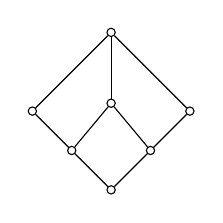
\begin{tikzpicture}[scale=0.5]
  \node[circle, minimum width=3pt, draw, inner sep=0pt] (1) at (0,2) {};
  \node[circle, minimum width=3pt, draw, inner sep=0pt] (p1) at (-2,0) {};
  \node[circle, minimum width=3pt, draw, inner sep=0pt] (t) at (0,0.2) {};
  \node[circle, minimum width=3pt, draw, inner sep=0pt] (p2) at (2,0) {};
  \node[circle, minimum width=3pt, draw, inner sep=0pt] (t1) at (-1,-1) {};
  \node[circle, minimum width=3pt, draw, inner sep=0pt] (t2) at (1,-1) {};
  \node[circle, minimum width=3pt, draw, inner sep=0pt] (0) at (0,-2) {};
  \draw (1) -- (p1) -- (t1) -- (0) -- (t2) -- (p2) -- (1);
  \draw (1) -- (t);
  \draw (t1) -- (t) -- (t2);
\end{tikzpicture}
\end{center}
The occurence of the lattice $\cD_2$ in $\Con(\bA^2)$ is not restricted to this particular example - the next result from \cite{hobby-mckenzie} shows that something like this occurs whenever we have a prime congruence quotient of type \textbf{5}.

\begin{prop}[Theorem 5.27 of \cite{hobby-mckenzie}] Suppose $(\alpha,\beta)$ is a nonabelian prime quotient on a finite algebra $\bA$ and let $\RR \le \bA^2$ be the basic tolerance for $(\alpha, \beta)$. Consider the sublattice
\[
\cL = \llbracket (\alpha \times \alpha)|_\RR, (\beta \times \beta)|_\RR \rrbracket
\]
of $\Con(\RR)$. If $(\alpha,\beta)$ has type \textbf{3} or \textbf{4} then $\cL$ is isomorphic to the four-element diamond lattice $\cM_2$, and if $(\alpha,\beta)$ has type \textbf{5} then $\cL$ is isomorphic to the lattice $\cD_2$ depicted above.
\end{prop}
\begin{proof} We can assume without loss of generality that $\alpha = 0_\bA$. Let $N$ be a $(0_\bA, \beta)$-trace, then $|N| = 2$ and $\bA|_N$ is polynomially equivalent to either a boolean algebra, a lattice, or a semilattice according to the type of $(0_\bA,\beta)$. Suppose $N = \{a,b\}$ and pick $e \in E(\bA)$ such that
\[
N = e(\bA) \cap a/\beta.
\]
Additionally, if $(0_\bA, \beta)$ has type \textbf{5} then assume that $a$ is the neutral element of $\bA|_N$ and that $b$ is the absorbing element.

First we check that each congruence on $(\bA|_N)^2$ extends to a congruence on $\RR$ which is contained in $(\beta \times \beta)|_\RR$. By Theorem \ref{thm-basic-tolerance}, we have
\[
\RR = \Sg_{\bA^2}(\Delta_\bA \cup N^2).
\]
Defining the unary polynomial $e^{(2)}$ on $\RR$ as in the proof of Proposition \ref{prop-restrict-variety}, we see that
\[
N^2 = e^{(2)}(\RR) \cap (a,a)/(\beta \times \beta)|_\RR,
\]
and $(\bA|_N)^2$ is polynomially equivalent to $\RR|_{N^2}$ by the argument of Proposition \ref{prop-restrict-variety}, so Lemma \ref{lem-idempotent-surjective-lattice} shows that restriction to $N^2$ defines a surjective lattice homomorphism from $\llbracket 0_\RR, (\beta \times \beta)|_\RR \rrbracket$ to $\Con((\bA|_N)^2)$.

The main difficulty is to check that every congruence $\theta$ on $\RR$ which is contained in $(\beta \times \beta)|_\RR$ is equal to $\Cg_\RR(\theta|_{N^2})$ - this requires some tedious casework. It's helpful to note that since the transitive closure of the tolerance $\RR$ is $\beta$, the congruence $(\beta \times \beta)|_\RR$ is actually the linking congruence of $\RR \le_{sd} \bA \times \bA$. In other words, we have
\[
(\beta \times \beta)|_\RR = \ker \pi_1 \vee \ker \pi_2.
\]
First we will show that the containment
\[
\Cg_\RR(\ker \pi_1|_{N^2}) \subseteq \ker \pi_1 = (0_\bA \times 1_\bA)|_\RR
\]
is an equality. Consider any $(c,d) \in \RR$. Since $\RR$ is generated by $\Delta_\bA \cup N^2$, there is some binary polynomial $p \in \Pol_2(\bA)$ such that $p(a,b) = c, p(b,a) = d$. Then we have
\[
\begin{bmatrix} c\\ d\end{bmatrix} = p\Big(\begin{bmatrix} a\\ b\end{bmatrix}, \begin{bmatrix} b\\ a\end{bmatrix}\Big) \equiv p\Big(\begin{bmatrix} a\\ a\end{bmatrix}, \begin{bmatrix} b\\ b\end{bmatrix}\Big) = \begin{bmatrix} c\\ c\end{bmatrix} \pmod{\Cg_\RR(\ker \pi_1|_{N^2})}.
\]
Since this is true for any $(c,d) \in \RR$, we see that $\Cg_\RR(\ker \pi_1|_{N^2}) = \ker \pi_1$.

Now for any $\theta \le (\beta \times \beta)|_\RR$, if $\pi_1(\theta) \ne \beta$ then $\theta \subseteq \ker \pi_1$ since $\beta$ is atomic. If $\pi_1(\theta) = \beta$, then $(a,b) \in \pi_1(e^{(2)}(\theta)) = \pi_1(\theta|_{N^2})$, so we have the implication
\[
\theta|_{N^2} \subseteq \ker \pi_1|_{N^2} \;\;\; \implies \;\;\; \theta \subseteq \ker \pi_1 = \Cg_\RR(\ker \pi_1|_{N^2}).
\]
Together with $\Cg_\RR(N^2) \supseteq \ker \pi_1 \vee \ker \pi_2$, this shows that $\theta = \Cg_\RR(\theta|_{N^2})$ if $\theta|_{N^2}$ is one of $0_N \times 0_N, 0_N \times 1_N, 1_N \times 0_N, 1_N\times 1_N$. This handles the cases where $(0_\bA, \beta)$ has type \textbf{3} or \textbf{4} (lattices and boolean algebras are congruence distributive, so congruences on $(\bA|_N)^2$ are determined by their first and second projections in these cases), so from here on we may assume that $(0_\bA, \beta)$ has type \textbf{5} (i.e. semilattice type).

By the analysis of the congruences on the square of the two-element semilattice from Example \ref{ex-con-semi-square}, we have two remaining cases: either $\theta|_{N^2}$ is the congruence generated by $((a,b), (b,a))$, or (possibly after swapping coordinates) $\theta|_{N^2}$ is the congruence generated by $((b,a),(b,b))$. In the first case, $\theta|_{N^2}$ contains both $((b,a),(b,b))$ and $((a,b),(b,b))$, so for any $(c,d) \in \RR$, if we choose the binary polynomial $p$ satisfying $p(a,b) = c, p(b,a) = d$ as before, we get
\[
\begin{bmatrix} c\\ d\end{bmatrix} = p\Big(\begin{bmatrix} a\\ b\end{bmatrix}, \begin{bmatrix} b\\ a\end{bmatrix}\Big) \equiv p\Big(\begin{bmatrix} b\\ b\end{bmatrix}, \begin{bmatrix} b\\ b\end{bmatrix}\Big) \in \Delta_\bA \pmod{\Cg_\RR(\theta|_{N^2})}.
\]
Thus in this case, every element of $\RR$ is congruent modulo $\theta$ to a diagonal element, so $\theta$ is determined by its restriction to $\Delta_\bA \cong \bA$. Since $\theta|_{\Delta_\bA} \subseteq (\beta \times \beta)|_{\Delta_\bA}$ and $(a,a)$ is not congruent to $(b,b)$ modulo $\theta$, we see that $\theta|_{\Delta_\bA}$ is trivial, so every pair of elements of $\RR$ which are congruent modulo $\theta$ are congruent to the same diagonal element of $\Delta_\bA$ via the congruence $\Cg_\RR\{((a,b),(b,a))\}$.

To finish the proof, we consider the case where $\theta|_{N^2}$ is the congruence generated by $((b,a),(b,b))$, so $\theta \subsetneq \ker \pi_1$. Suppose that the pairs $(c,d_1), (c,d_2) \in \RR$ are congruent modulo $\theta$, and choose binary polynomials $p_1,p_2$ such that $p_i(a,b) = c$ and $p_i(b,a) = d_i$. Then we have
\[
\begin{bmatrix} c\\ d_i\end{bmatrix} = p_i\Big(\begin{bmatrix} a\\ b\end{bmatrix}, \begin{bmatrix} b\\ a\end{bmatrix}\Big) \equiv p_i\Big(\begin{bmatrix} a\\ b\end{bmatrix}, \begin{bmatrix} b\\ b\end{bmatrix}\Big) = \begin{bmatrix} c\\ p_i(b,b)\end{bmatrix} \pmod{\Cg_\RR(\theta|_{N^2})}.
\]
We claim that $p_1(b,b) = p_2(b,b)$. Suppose not, for the sake of contradiction. Since $p_1(b,b) \ne p_2(b,b) \in c/\beta$, we can apply Theorem \ref{thm-minimal-sets}(c) to see that there is some unary $f \in \Pol_1(\bA)$ such that $f(p_1(b,b)) \ne f(p_2(b,b))$ and $f(c/\beta) = N$. Suppose without loss of generality that $f(p_1(b,b)) = a$, and note that since $(a,a)$ is not congruent to $(a,b)$ modulo $\theta$ we must have $f(c) = b$. Then the unary polynomial $g(x) = f(p_1(x,b))$ preserves $N$ and satisfies
\[
g(b) = f(p_1(b,b)) = a, \;\;\; g(a) = f(p_1(a,b)) = f(c) = b.
\]
Then $g|_N$ is not monotone, which contradicts the assumption that $\bA|_N$ is polynomially equivalent to a semilattice, so we must have had $p_1(b,b) = p_2(b,b)$ after all. Therefore $(c,d_1)$ is congruent to $(c,d_2)$ modulo $\Cg_\RR(\theta|_{N^2})$, and since this is true for any $(c,d_1),(c,d_2)$ which are congruent modulo $\theta$, we are done.
\end{proof}

The fact that prime congruences of types \textbf{3} and \textbf{4} have dual weak pseudocomplements has a nice concrete consequence.

\begin{prop} If $\bB$ is a finite simple algebra of boolean or lattice type (i.e., if $(0_\bB,1_\bB)$ has type \textbf{3} or \textbf{4}), then for any finite collection of finite algebras $\bA_i$, if $\bB \in \cV(\bA_1, ..., \bA_n)$ then $\bB \in HS(\bA_i)$ for some $i$.
\end{prop}
\begin{proof} Since $\bB, \bA_i$ are finite, if $\bB \in \cV(\bA_1, ..., \bA_n)$ then $\bB \in HSP_{fin}(\bA_1, ..., \bA_n)$, so there is some $\RR \le \prod_i \bA_i^{k_i}$ and some congruence $\theta \in \Con(\RR)$ such that $\bB \cong \RR/\theta$. Assume for simplicity that the $k_i$ are all $1$, by repeating some of the $\bA_i$s if necessary. We just need to prove that $\ker \pi_i \le \theta$ for some $i$ to complete the proof, since then $\bB$ will be isomorphic to a quotient of $\pi_i(\RR) \le \bA_i$.

By Proposition \ref{prop-tame-quotient}, the prime quotient $(\theta,1_\RR)$ has the same type as $(0_\bB,1_\bB)$, so by Proposition \ref{prop-dual-weak-pseudo} we see that $\theta$ has a dual weak pseudocomplement $\delta$ under $1_\RR$. If every $i$ has $\ker \pi_i \not\le \theta$, then each $i$ has $\theta \vee \ker \pi_1 = 1_\RR$, in which case we must have $\delta \le \ker \pi_i$ for all $i$. But then we have $\delta = 0_\RR$, which contradicts $\theta \vee \delta = 1_\RR$.
\end{proof}

Even though prime congruences of type \textbf{5} might not have dual weak pseudocomplements in general, the fact that they always have weak pseudocomplements can be use to prove that they have dual weak pseudocomplements in some special cases.

\begin{prop} If $(\alpha,\beta)$ is a nonabelian prime quotient on a finite algebra $\bA$, and if there is some $\gamma$ such that $\alpha \vee \gamma = \beta$ and $\alpha \wedge \gamma = 0_\bA$, then $\alpha$ has a dual weak pseudocomplement under $\beta$.

More generally, any nonabelian prime quotient $(\alpha,\beta)$ of $\bA$ has the following property: for all $\gamma$ such that $\alpha \vee \gamma = \beta$, there is a least $\delta$ such that $\alpha \vee \delta = \beta$ and $\alpha \wedge \gamma \le \delta$.
\end{prop}
\begin{proof} The more general statement follows from the first statement by replacing $\bA$ by $\bA/(\alpha \wedge \gamma)$, so suppose that $\alpha \vee \gamma = \beta$ and $\alpha \wedge \gamma = 0_\bA$.

Let $\delta$ be any atom of the lattice $\llbracket 0_\bA, \gamma \rrbracket$. Then we have
\[
\alpha \wedge \delta \le \alpha \wedge \gamma = 0_\bA
\]
and
\[
\delta \not\le \alpha, \;\;\; \delta \le \gamma \le \beta \;\;\; \implies \;\;\; \alpha \vee \delta = \beta.
\]
Thus the prime congruence quotient $(0_\bA,\delta)$ is perspective to $(\alpha,\beta)$, so it must be nonabelian since $\stackrel{s}{\sim}$ is a congruence on $\Con(\bA)$ by Theorem \ref{thm-locally-solvable-congruence} (in fact $(0_\bA,\delta)$ has the same type as $(\alpha,\beta)$ by Proposition \ref{prop-minimal-sets-perspective}).

By Proposition \ref{prop-centralizer-pseudocomplement}, $\delta$ has a pseudocomplement $(0_\bA : \delta)$. Then for any $\theta$ such that $\delta \not\le \theta$ we have
\[
\delta \wedge \theta = 0_\bA,
\]
and together with $\alpha \wedge \delta = 0_\bA$ we see that
\[
\alpha \vee \theta \le (0_\bA : \delta).
\]
Since $\delta \le \beta$ we have $\beta \not\le (0_\bA : \delta)$, so we have proven that
\[
\delta \not\le \theta \;\;\; \implies \;\;\; \alpha \vee \theta \ne \beta.
\]
Thus $\delta$ is the dual weak pseudocomplement of $\alpha$ under $\beta$.
\end{proof}

Putting together the results we have shown so far, we can give a sufficient condition for intervals in $\Con(\bA)$ to be congruence semidistributive.

\begin{prop} If $\bA$ is a finite algebra and $\alpha \le \beta \in \Con(\bA)$, then
\begin{itemize}
\item if no prime congruence quotient $(\gamma,\delta)$ with $\alpha \le \gamma \prec \delta \le \beta$ has type \textbf{1} or \textbf{2}, then $\llbracket \alpha, \beta \rrbracket$ is meet-semidistributive, and

\item if no prime congruence quotient $(\gamma,\delta)$ with $\alpha \le \gamma \prec \delta \le \beta$ has type \textbf{1}, \textbf{2}, or \textbf{5}, then $\llbracket \alpha, \beta \rrbracket$ is join-semidistributive.
\end{itemize}
\end{prop}
\begin{proof} This follows from Proposition \ref{prop-semidistributive-prime-pseudocomplement}, Proposition \ref{prop-centralizer-pseudocomplement}, and Proposition \ref{prop-dual-weak-pseudo}.
\end{proof}

We can prove much stronger results by making use of the congruence $\stackrel{s}{\sim}$ on $\Con(\bA)$.

\begin{thm} If $\bA$ is locally finite, then $\Con(\bA)/\!\stackrel{s}{\sim}$ satisfies the infinite meet-semidistributivity law \eqref{infinite-meet-semidistributive-law}.
\end{thm}
\begin{proof} Suppose that $\alpha, \beta_i \in \Con(\bA)$ satisfy $\alpha \wedge \beta_i \stackrel{s}{\sim} \alpha \wedge \beta_j$ for all $i,j$. By Proposition \ref{prop-solvable-quotient-algebraic}, we may assume without loss of generality that each $\beta_i$ is the join of all the elements of its $\stackrel{s}{\sim}$-class, in which case we must actually have
\[
\alpha \wedge \beta_i = \alpha \wedge \beta_j
\]
for all $i,j$. Let $\delta$ be the common value of $\alpha \wedge \beta_i$. By Proposition \ref{gen-commutator}(b), we have
\[
\alpha \wedge \beta_i = \delta \;\;\; \implies \;\;\; C(\beta_i, \alpha; \delta)
\]
for all $i$, so by Proposition \ref{gen-commutator}(e) we have
\[
C\big(\bigvee_i \beta_i, \alpha; \delta\big).
\]
Then by Proposition \ref{gen-commutator}(c) $\alpha \wedge \big(\bigvee_i \beta_i\big)$ is abelian over $\delta$, which implies $\alpha \wedge \big(\bigvee_i \beta_i\big) \stackrel{s}{\sim} \delta$.
\begin{comment}
By Proposition \ref{prop-solvable-quotient-algebraic}, $\Con(\bA)/\!\stackrel{s}{\sim}$ is an algebraic lattice, so we can apply Proposition \ref{prop-infinite-semidistributive-algebraic} to see that $\Con(\bA)/\!\stackrel{s}{\sim}$ satisfies \eqref{infinite-meet-semidistributive-law} iff it is meet-semidistributive.

Suppose for the sake of contradiction that there are $\alpha, \beta, \gamma \in \Con(\bA)$ such that $\alpha \wedge \beta \stackrel{s}{\sim} \alpha \wedge \gamma$ but
\[
\alpha \wedge (\beta \vee \gamma) \not\stackrel{s}{\sim} \alpha \wedge \beta.
\]
Then by the definition of $\stackrel{s}{\sim}$ there is some pair $(a,b) \in \Sn_2(\bA)$ which is contained in $\alpha \wedge (\beta \vee \gamma)$, but which is not contained in $\alpha \wedge \beta$. Since $(a,b) \in \beta \vee \gamma$, there is some $k$ such that $(a,b) \in (\beta \circ \gamma)^{\circ k}$, so there is a finitely generated subalgebra $\bB$ of $\bA$ which contains $a,b$ and the elements along some $\beta,\gamma$ path from $a$ to $b$ such that
\[
(a,b) \in \alpha|_\bB \wedge (\beta|_\bB \vee \gamma|_\bB).
\]
By ensuring that $\bB$ contains the constants needed to define a binary polynomial $s$ such that $(\{a,b\},s)$ is a semilattice, we can also ensure that $(a,b) \in \Sn_2(\bB)$, so
\[
\alpha|_\bB \wedge (\beta|_\bB \vee \gamma|_\bB) \not\stackrel{s}{\sim} \alpha|_\bB \wedge \beta|_\bB.
\]
Thus we may assume without loss of generality that $\bA$ is finite.
\end{comment}
\end{proof}

\begin{thm} If $\bA$ is finite and a convex sublattice $\cL \le \Con(\bA)$ contains no prime congruence quotients of type \textbf{5}, then $\cL/\!\!\stackrel{s}{\sim}$ is semidistributive (i.e. both meet-semidistributive and join-semidistributive).
\end{thm}
\begin{proof} We've already shown that $\cL/\!\stackrel{s}{\sim}$ is meet-semidistributive, so we only need to check that it is join-semidistributive. Suppose that $\alpha, \beta, \gamma \in \cL$ satisfy $\alpha \vee \beta \stackrel{s}{\sim} \alpha \vee \gamma$. We can assume without loss of generality that $\alpha$ is minimal in $\alpha/\!\stackrel{s}{\sim} \cap \cL$, and similarly for $\beta$ and $\gamma$, in which case we actually have
\[
\alpha \vee \beta = \alpha \vee \gamma,
\]
and if we call the common value $\delta$ then $\delta$ is minimal in $\delta/\!\!\stackrel{s}{\sim} \cap \cL$. If we assume for the sake of contradiction that $\alpha \vee (\beta \wedge \gamma) \ne \delta$, then there is some prime congruence quotient $(\epsilon,\delta)$ such that
\[
\alpha \vee (\beta \wedge \gamma) \le \epsilon \prec \delta,
\]
and by the dual to Proposition \ref{prop-semidistributive-prime-pseudocomplement} there can't be any dual weak pseudocomplement to $\epsilon$ under $\delta$. Since $\epsilon \in \cL$ and $\delta$ is minimal in $\delta/\!\stackrel{s}{\sim} \cap \cL$, we see that $\epsilon \not\stackrel{s}{\sim} \delta$, and by our assumption on $\cL$ the type of $(\epsilon,\delta)$ must therefore be \textbf{3} or \textbf{4}, contradicting Proposition \ref{prop-dual-weak-pseudo}.
\end{proof}


%\section{Locally finite congruence modular varieties}
%TODO


%\section{Omitting types}
%TODO


\end{appendices}

